\documentclass[twoside]{book}

% Packages required by doxygen
\usepackage{fixltx2e}
\usepackage{calc}
\usepackage{doxygen}
\usepackage[export]{adjustbox} % also loads graphicx
\usepackage{graphicx}
\usepackage[utf8]{inputenc}
\usepackage{makeidx}
\usepackage{multicol}
\usepackage{multirow}
\PassOptionsToPackage{warn}{textcomp}
\usepackage{textcomp}
\usepackage[nointegrals]{wasysym}
\usepackage[table]{xcolor}

% Font selection
\usepackage[T1]{fontenc}
\usepackage[scaled=.90]{helvet}
\usepackage{courier}
\usepackage{amssymb}
\usepackage{sectsty}
\renewcommand{\familydefault}{\sfdefault}
\allsectionsfont{%
  \fontseries{bc}\selectfont%
  \color{darkgray}%
}
\renewcommand{\DoxyLabelFont}{%
  \fontseries{bc}\selectfont%
  \color{darkgray}%
}
\newcommand{\+}{\discretionary{\mbox{\scriptsize$\hookleftarrow$}}{}{}}

% Page & text layout
\usepackage{geometry}
\geometry{%
  a4paper,%
  top=2.5cm,%
  bottom=2.5cm,%
  left=2.5cm,%
  right=2.5cm%
}
\tolerance=750
\hfuzz=15pt
\hbadness=750
\setlength{\emergencystretch}{15pt}
\setlength{\parindent}{0cm}
\setlength{\parskip}{3ex plus 2ex minus 2ex}
\makeatletter
\renewcommand{\paragraph}{%
  \@startsection{paragraph}{4}{0ex}{-1.0ex}{1.0ex}{%
    \normalfont\normalsize\bfseries\SS@parafont%
  }%
}
\renewcommand{\subparagraph}{%
  \@startsection{subparagraph}{5}{0ex}{-1.0ex}{1.0ex}{%
    \normalfont\normalsize\bfseries\SS@subparafont%
  }%
}
\makeatother

% Headers & footers
\usepackage{fancyhdr}
\pagestyle{fancyplain}
\fancyhead[LE]{\fancyplain{}{\bfseries\thepage}}
\fancyhead[CE]{\fancyplain{}{}}
\fancyhead[RE]{\fancyplain{}{\bfseries\leftmark}}
\fancyhead[LO]{\fancyplain{}{\bfseries\rightmark}}
\fancyhead[CO]{\fancyplain{}{}}
\fancyhead[RO]{\fancyplain{}{\bfseries\thepage}}
\fancyfoot[LE]{\fancyplain{}{}}
\fancyfoot[CE]{\fancyplain{}{}}
\fancyfoot[RE]{\fancyplain{}{\bfseries\scriptsize Generated by Doxygen }}
\fancyfoot[LO]{\fancyplain{}{\bfseries\scriptsize Generated by Doxygen }}
\fancyfoot[CO]{\fancyplain{}{}}
\fancyfoot[RO]{\fancyplain{}{}}
\renewcommand{\footrulewidth}{0.4pt}
\renewcommand{\chaptermark}[1]{%
  \markboth{#1}{}%
}
\renewcommand{\sectionmark}[1]{%
  \markright{\thesection\ #1}%
}

% Indices & bibliography
\usepackage{natbib}
\usepackage[titles]{tocloft}
\setcounter{tocdepth}{3}
\setcounter{secnumdepth}{5}
\makeindex

% Hyperlinks (required, but should be loaded last)
\usepackage{ifpdf}
\ifpdf
  \usepackage[pdftex,pagebackref=true]{hyperref}
\else
  \usepackage[ps2pdf,pagebackref=true]{hyperref}
\fi
\hypersetup{%
  colorlinks=true,%
  linkcolor=blue,%
  citecolor=blue,%
  unicode%
}

% Custom commands
\newcommand{\clearemptydoublepage}{%
  \newpage{\pagestyle{empty}\cleardoublepage}%
}

\usepackage{caption}
\captionsetup{labelsep=space,justification=centering,font={bf},singlelinecheck=off,skip=4pt,position=top}

%===== C O N T E N T S =====

\begin{document}

% Titlepage & ToC
\hypersetup{pageanchor=false,
             bookmarksnumbered=true,
             pdfencoding=unicode
            }
\pagenumbering{roman}
\begin{titlepage}
\vspace*{7cm}
\begin{center}%
{\Large Ci\+A402\+Device }\\
\vspace*{1cm}
{\large Generated by Doxygen 1.8.11}\\
\end{center}
\end{titlepage}
\clearemptydoublepage
\tableofcontents
\clearemptydoublepage
\pagenumbering{arabic}
\hypersetup{pageanchor=true}

%--- Begin generated contents ---
\chapter{Ci\+A402\+Device}
\label{index}\hypertarget{index}{}Library under CiA 402 standard for device control

\section*{How to use}

This library is intended for the use with C\+Make build system and Socket\+Can hardware. Under C\+Make building, it automatically holds all the include and link directories in variables\+:


\begin{DoxyCode}
1 SUBDIR\_INCLUDE\_DIRECTORIES
2 SUBDIR\_LINK\_NAMES
\end{DoxyCode}


Then, assuming the library is placed at \char`\"{}\$\{\+P\+R\+O\+J\+E\+C\+T\+\_\+\+S\+O\+U\+R\+C\+E\+\_\+\+D\+I\+R\}/lib/\+Ci\+A402\+Device/\char`\"{} (for example after clone with {\ttfamily git clone \href{https://github.com/HUMASoft/CiA402Device.git}{\tt https\+://github.\+com/\+H\+U\+M\+A\+Soft/\+Ci\+A402\+Device.\+git}}, it is enough to add the following lines to \hyperlink{CMakeLists_8txt}{C\+Make\+Lists.\+txt} to add includes\+:


\begin{DoxyCode}
1 add\_subdirectory($\{PROJECT\_SOURCE\_DIR\}/lib/CiA402Device/)
2 INCLUDE\_DIRECTORIES($\{SUBDIR\_INCLUDE\_DIRECTORIES\})
\end{DoxyCode}


Also after \char`\"{}add\+\_\+executable( \$\{name\} \$\{sourcefile\} )\char`\"{} line, add the following to link the library\+:


\begin{DoxyCode}
1 target\_link\_libraries( $\{PROJECT\_NAME\} $\{SUBDIR\_LINK\_NAMES\} )
\end{DoxyCode}


\section*{Can interface}

Remember to start can interface by typing these lines\+:


\begin{DoxyCode}
1 sudo ip link add dev can0 type can
2 sudo ip link set up can0
\end{DoxyCode}


\section*{Main classes}

The library is based on the use of the class {\ttfamily \hyperlink{classCiA402Device}{Ci\+A402\+Device}}, then the use of the functionalities will be done trough an instance of that class. A communication port is also needed, so the commo instance will be done with the following lines\+:


\begin{DoxyCode}
\textcolor{comment}{//prepare port. Open a port address with a PortBase Object}
\hyperlink{classSocketCanPort}{SocketCanPort} p1(\textcolor{stringliteral}{"can0"});

\textcolor{comment}{//Create a joint and give a canopen id, and a 301port (by constructor)}
\hyperlink{classCiA402Device}{CiA402Device} j1(3,&p1);
\end{DoxyCode}


See \href{https://github.com/HUMASoft/CiA402Device-example}{\tt https\+://github.\+com/\+H\+U\+M\+A\+Soft/\+Ci\+A402\+Device-\/example} for more use examples.

Troubleshooting here\+: \href{https://github.com/HUMASoft/CiA402Device/wiki/Troubleshooting}{\tt https\+://github.\+com/\+H\+U\+M\+A\+Soft/\+Ci\+A402\+Device/wiki/\+Troubleshooting}.

\section*{Collaboration graph}

 
\chapter{Namespace Index}
\section{Namespace List}
Here is a list of all namespaces with brief descriptions\+:\begin{DoxyCompactList}
\item\contentsline{section}{\hyperlink{namespacenmt}{nmt} }{\pageref{namespacenmt}}{}
\item\contentsline{section}{\hyperlink{namespaceod}{od} }{\pageref{namespaceod}}{}
\item\contentsline{section}{\hyperlink{namespacepdo}{pdo} }{\pageref{namespacepdo}}{}
\item\contentsline{section}{\hyperlink{namespacesdo}{sdo} }{\pageref{namespacesdo}}{}
\end{DoxyCompactList}

\chapter{Hierarchical Index}
\section{Class Hierarchy}
This inheritance list is sorted roughly, but not completely, alphabetically\+:\begin{DoxyCompactList}
\item \contentsline{section}{can\+\_\+filter}{\pageref{structcan__filter}}{}
\item \contentsline{section}{can\+\_\+msg}{\pageref{structcan__msg}}{}
\item \contentsline{section}{Ci\+A301\+Comm\+Port}{\pageref{classCiA301CommPort}}{}
\begin{DoxyCompactList}
\item \contentsline{section}{Ci\+A402\+Device}{\pageref{classCiA402Device}}{}
\end{DoxyCompactList}
\item \contentsline{section}{Ci\+A402\+Device\+I\+Canbus}{\pageref{classCiA402DeviceICanbus}}{}
\item \contentsline{section}{Ci\+A402\+Setup\+Data}{\pageref{classCiA402SetupData}}{}
\item \contentsline{section}{co\+\_\+msg}{\pageref{structco__msg}}{}
\item \contentsline{section}{Device\+Chain}{\pageref{classDeviceChain}}{}
\item \contentsline{section}{err\+\_\+stat}{\pageref{structerr__stat}}{}
\item \contentsline{section}{Port\+Base}{\pageref{classPortBase}}{}
\begin{DoxyCompactList}
\item \contentsline{section}{Can\+Bus\+Port}{\pageref{classCanBusPort}}{}
\item \contentsline{section}{Socket\+Can\+Port}{\pageref{classSocketCanPort}}{}
\item \contentsline{section}{Test\+Port}{\pageref{classTestPort}}{}
\end{DoxyCompactList}
\end{DoxyCompactList}

\chapter{Class Index}
\doxysection{Class List}
Here are the classes, structs, unions and interfaces with brief descriptions\+:\begin{DoxyCompactList}
\item\contentsline{section}{\mbox{\hyperlink{classBaseBlock}{Base\+Block}} }{\pageref{classBaseBlock}}{}
\item\contentsline{section}{\mbox{\hyperlink{classBlockDiagram}{Block\+Diagram}} }{\pageref{classBlockDiagram}}{}
\item\contentsline{section}{\mbox{\hyperlink{classControllerBlock}{Controller\+Block}} }{\pageref{classControllerBlock}}{}
\item\contentsline{section}{\mbox{\hyperlink{classFactorSystemBlock}{Factor\+System\+Block}} }{\pageref{classFactorSystemBlock}}{}
\item\contentsline{section}{\mbox{\hyperlink{classFPDBlock}{FPDBlock}} }{\pageref{classFPDBlock}}{}
\item\contentsline{section}{\mbox{\hyperlink{classFPDTuner}{FPDTuner}} }{\pageref{classFPDTuner}}{}
\item\contentsline{section}{\mbox{\hyperlink{classFractionalController1DOF}{Fractional\+Controller1\+DOF}} }{\pageref{classFractionalController1DOF}}{}
\item\contentsline{section}{\mbox{\hyperlink{classFractionalDerivative}{Fractional\+Derivative}} }{\pageref{classFractionalDerivative}}{}
\item\contentsline{section}{\mbox{\hyperlink{classFSystemBlock}{FSystem\+Block}} }{\pageref{classFSystemBlock}}{}
\item\contentsline{section}{\mbox{\hyperlink{classKalmanFilter}{Kalman\+Filter}} \\*The \mbox{\hyperlink{classKalmanFilter}{Kalman\+Filter}} class\+: This class its implements a filter based in Kalman }{\pageref{classKalmanFilter}}{}
\item\contentsline{section}{\mbox{\hyperlink{classLinearSystem}{Linear\+System}} }{\pageref{classLinearSystem}}{}
\item\contentsline{section}{\mbox{\hyperlink{classOnlineSystemIdentification}{Online\+System\+Identification}} \\*The \mbox{\hyperlink{classOnlineSystemIdentification}{Online\+System\+Identification}} class is the base class for all the online system identification strategies. Recursive least squares is implemented and can be used, but any other methods can be implemented using inheritance and method overload (polymorphism) }{\pageref{classOnlineSystemIdentification}}{}
\item\contentsline{section}{\mbox{\hyperlink{classPIDBlock}{PIDBlock}} }{\pageref{classPIDBlock}}{}
\item\contentsline{section}{\mbox{\hyperlink{classSamplingTime}{Sampling\+Time}} }{\pageref{classSamplingTime}}{}
\item\contentsline{section}{\mbox{\hyperlink{classSignalSum}{Signal\+Sum}} }{\pageref{classSignalSum}}{}
\item\contentsline{section}{\mbox{\hyperlink{classStateSpace}{State\+Space}} }{\pageref{classStateSpace}}{}
\item\contentsline{section}{\mbox{\hyperlink{classStateVariable}{State\+Variable}} }{\pageref{classStateVariable}}{}
\item\contentsline{section}{\mbox{\hyperlink{classStateVariableBlock}{State\+Variable\+Block}} }{\pageref{classStateVariableBlock}}{}
\item\contentsline{section}{\mbox{\hyperlink{classSystemBlock}{System\+Block}} \\*The \mbox{\hyperlink{classSystemBlock}{System\+Block}} class\+: This class encapsulates a system control block, defined by its transference function G. }{\pageref{classSystemBlock}}{}
\item\contentsline{section}{\mbox{\hyperlink{classSystemBlockChain}{System\+Block\+Chain}} }{\pageref{classSystemBlockChain}}{}
\item\contentsline{section}{\mbox{\hyperlink{classSystemTF}{System\+TF}} \\*The \mbox{\hyperlink{classSystemBlock}{System\+Block}} class\+: This class encapsulates a system control block, defined by its transference function G. }{\pageref{classSystemTF}}{}
\item\contentsline{section}{\mbox{\hyperlink{classTableInterpolation}{Table\+Interpolation}} }{\pageref{classTableInterpolation}}{}
\item\contentsline{section}{\mbox{\hyperlink{classTimeSignal}{Time\+Signal}} }{\pageref{classTimeSignal}}{}
\item\contentsline{section}{\mbox{\hyperlink{classTransferFunction}{Transfer\+Function}} }{\pageref{classTransferFunction}}{}
\end{DoxyCompactList}

\chapter{File Index}
\section{File List}
Here is a list of all files with brief descriptions\+:\begin{DoxyCompactList}
\item\contentsline{section}{\hyperlink{CanBusPort_8cpp}{Can\+Bus\+Port.\+cpp} }{\pageref{CanBusPort_8cpp}}{}
\item\contentsline{section}{\hyperlink{CanBusPort_8h}{Can\+Bus\+Port.\+h} }{\pageref{CanBusPort_8h}}{}
\item\contentsline{section}{\hyperlink{candatatypes_8h}{candatatypes.\+h} }{\pageref{candatatypes_8h}}{}
\item\contentsline{section}{\hyperlink{CiA301CommPort_8cpp}{Ci\+A301\+Comm\+Port.\+cpp} }{\pageref{CiA301CommPort_8cpp}}{}
\item\contentsline{section}{\hyperlink{CiA301CommPort_8h}{Ci\+A301\+Comm\+Port.\+h} }{\pageref{CiA301CommPort_8h}}{}
\item\contentsline{section}{\hyperlink{Cia402device_8cpp}{Cia402device.\+cpp} }{\pageref{Cia402device_8cpp}}{}
\item\contentsline{section}{\hyperlink{Cia402device_8h}{Cia402device.\+h} }{\pageref{Cia402device_8h}}{}
\item\contentsline{section}{\hyperlink{CiA402DeviceICanbus_8cpp}{Ci\+A402\+Device\+I\+Canbus.\+cpp} }{\pageref{CiA402DeviceICanbus_8cpp}}{}
\item\contentsline{section}{\hyperlink{CiA402DeviceICanbus_8h}{Ci\+A402\+Device\+I\+Canbus.\+h} }{\pageref{CiA402DeviceICanbus_8h}}{}
\item\contentsline{section}{\hyperlink{CiA402SetupData_8cpp}{Ci\+A402\+Setup\+Data.\+cpp} }{\pageref{CiA402SetupData_8cpp}}{}
\item\contentsline{section}{\hyperlink{CiA402SetupData_8h}{Ci\+A402\+Setup\+Data.\+h} }{\pageref{CiA402SetupData_8h}}{}
\item\contentsline{section}{\hyperlink{co__msg_8h}{co\+\_\+msg.\+h} }{\pageref{co__msg_8h}}{}
\item\contentsline{section}{\hyperlink{DeviceChain_8cpp}{Device\+Chain.\+cpp} }{\pageref{DeviceChain_8cpp}}{}
\item\contentsline{section}{\hyperlink{DeviceChain_8h}{Device\+Chain.\+h} }{\pageref{DeviceChain_8h}}{}
\item\contentsline{section}{\hyperlink{hico__api_8h}{hico\+\_\+api.\+h} }{\pageref{hico__api_8h}}{}
\item\contentsline{section}{\hyperlink{ObjectDictionary_8h}{Object\+Dictionary.\+h} }{\pageref{ObjectDictionary_8h}}{}
\item\contentsline{section}{\hyperlink{PortBase_8cpp}{Port\+Base.\+cpp} }{\pageref{PortBase_8cpp}}{}
\item\contentsline{section}{\hyperlink{PortBase_8h}{Port\+Base.\+h} }{\pageref{PortBase_8h}}{}
\item\contentsline{section}{\hyperlink{SocketCanPort_8cpp}{Socket\+Can\+Port.\+cpp} }{\pageref{SocketCanPort_8cpp}}{}
\item\contentsline{section}{\hyperlink{SocketCanPort_8h}{Socket\+Can\+Port.\+h} }{\pageref{SocketCanPort_8h}}{}
\item\contentsline{section}{\hyperlink{TestPort_8cpp}{Test\+Port.\+cpp} }{\pageref{TestPort_8cpp}}{}
\item\contentsline{section}{\hyperlink{TestPort_8h}{Test\+Port.\+h} }{\pageref{TestPort_8h}}{}
\end{DoxyCompactList}

\chapter{Namespace Documentation}
\hypertarget{namespacenmt}{}\section{nmt Namespace Reference}
\label{namespacenmt}\index{nmt@{nmt}}
\subsection*{Variables}
\begin{DoxyCompactItemize}
\item 
const vector$<$ uint8\+\_\+t $>$ \hyperlink{namespacenmt_a1310e5c59553352490180a42ef1dad8c}{started} =\{0x01\}
\end{DoxyCompactItemize}


\subsection{Variable Documentation}
\index{nmt@{nmt}!started@{started}}
\index{started@{started}!nmt@{nmt}}
\subsubsection[{\texorpdfstring{started}{started}}]{\setlength{\rightskip}{0pt plus 5cm}const vector$<$uint8\+\_\+t$>$ nmt\+::started =\{0x01\}}\hypertarget{namespacenmt_a1310e5c59553352490180a42ef1dad8c}{}\label{namespacenmt_a1310e5c59553352490180a42ef1dad8c}

\hypertarget{namespaceod}{}\section{od Namespace Reference}
\label{namespaceod}\index{od@{od}}
\subsection*{Variables}
\begin{DoxyCompactItemize}
\item 
const vector$<$ uint8\+\_\+t $>$ \hyperlink{namespaceod_acb23d3cf4cdb0ce0c85a884a5a97ac00}{controlword} =\{0x40,0x60\}
\item 
const vector$<$ uint8\+\_\+t $>$ \hyperlink{namespaceod_a7fe65fca00afb38d66fb49ec4fdc88c0}{statusword} =\{0x41,0x60\}
\item 
const vector$<$ uint8\+\_\+t $>$ \hyperlink{namespaceod_a75b2ed7fb6e21d4335334e1525fd223c}{commreset} =\{0x81\}
\item 
const vector$<$ uint8\+\_\+t $>$ \hyperlink{namespaceod_af9d6d0e820d6bc1ee375195e253f7b7b}{fullreset} =\{0x82\}
\item 
const vector$<$ uint8\+\_\+t $>$ \hyperlink{namespaceod_a5ca62a6451017dd2a0d53391d6fc5161}{start} =\{0x01\}
\item 
const vector$<$ uint8\+\_\+t $>$ \hyperlink{namespaceod_a360cf2eae7cc59f7bd224fcf5992c767}{goreadytoswitchon} =\{0x06,0x00\}
\item 
const vector$<$ uint8\+\_\+t $>$ \hyperlink{namespaceod_a933f995790a17f6cdd3b54df8f7483a6}{goswitchon} =\{0x07,0x00\}
\item 
const vector$<$ uint8\+\_\+t $>$ \hyperlink{namespaceod_a74448ee88df5960df4c32613e7cdcd53}{goenable} =\{0x0\+F,0x00\}
\item 
const vector$<$ uint8\+\_\+t $>$ \hyperlink{namespaceod_a12f3001ff096334fecb9c9749be4d1c2}{goswitchondisable} =\{0x00,0x00\}
\item 
const vector$<$ uint8\+\_\+t $>$ \hyperlink{namespaceod_af47128107b86d08e437f81d48d20b05a}{run} =\{0x1\+F,0x00\}
\item 
const vector$<$ uint8\+\_\+t $>$ \hyperlink{namespaceod_ae572be966c7d5de90544f2ac32dbbd38}{expedite} =\{0x3\+F,0x00\}
\item 
const vector$<$ uint8\+\_\+t $>$ \hyperlink{namespaceod_a9afdc654634df7cc336d824c594d484a}{quickstop} =\{0x02,0x00\}
\item 
const vector$<$ uint8\+\_\+t $>$ \hyperlink{namespaceod_a6f4fb30463057c20b9374a69826f6143}{Operation\+Mode} =\{0x60,0x60,0x00\}
\item 
const vector$<$ uint8\+\_\+t $>$ \hyperlink{namespaceod_a0469b45cd9158b638f0e0d6ed1102742}{Operation\+Mode\+Display} =\{0x61,0x60,0x00\}
\item 
const vector$<$ uint8\+\_\+t $>$ \hyperlink{namespaceod_a85efca0656a6714d7227858e112c4a73}{positionmode} =\{0x01\}
\item 
const vector$<$ uint8\+\_\+t $>$ \hyperlink{namespaceod_a2771fb30adf397c1cd2ddb092a414e82}{velocitymode} =\{0x03\}
\item 
const vector$<$ uint8\+\_\+t $>$ \hyperlink{namespaceod_ab5b4d34058d08a758277bf52cd31d8c9}{quick\+\_\+stop\+\_\+mode} =\{0x5\+A,0x60\}
\item 
const vector$<$ uint8\+\_\+t $>$ \hyperlink{namespaceod_af1bc07726906ffc6ea25ab9abb478143}{stop\+\_\+option\+\_\+code} =\{0x5\+D,0x60\}
\item 
const vector$<$ uint8\+\_\+t $>$ \hyperlink{namespaceod_ac4b980a10ae256ea019a767459b6ba9b}{checkerror} =\{0x02,0x10\}
\item 
const vector$<$ uint8\+\_\+t $>$ \hyperlink{namespaceod_a716df35f1a3cc3e1792c033be7fc0518}{positionaddress} =\{0x64,0x60,0x00\}
\item 
const vector$<$ uint8\+\_\+t $>$ \hyperlink{namespaceod_ad2c386d1f9bfc49b8a247f0b093f8963}{velocityactvalue} =\{0x69,0x60\}
\item 
const vector$<$ uint8\+\_\+t $>$ \hyperlink{namespaceod_adf45781fb80275c184d548ea793b376b}{velocityaddress} =\{0x69,0x60\}
\item 
const vector$<$ uint8\+\_\+t $>$ \hyperlink{namespaceod_a0bdcdb539c588cfae0d43cc0ba40ea05}{target\+\_\+position} =\{0x7\+A,0x60,0x00\}
\item 
const vector$<$ uint8\+\_\+t $>$ \hyperlink{namespaceod_a1d5963cb8a002987c96fae2e172790ee}{position\+\_\+demand} =\{0x62,0x60,0x00\}
\item 
const vector$<$ uint8\+\_\+t $>$ \hyperlink{namespaceod_a53c06ba9dc3fe72c8fd5fed43563a4a0}{torquemode} =\{0x\+F\+B\}
\item 
const vector$<$ uint8\+\_\+t $>$ \hyperlink{namespaceod_afc052d3983ca0866a0b8cd5d0fc5deaa}{torque\+\_\+type\+\_\+extern} =\{0x1\+D,0x20,0x00\}
\item 
const vector$<$ uint8\+\_\+t $>$ \hyperlink{namespaceod_ada58f32a60ef9137c7e9c4f4f54ace10}{torque\+\_\+online} =\{0x01,0x00\}
\item 
const vector$<$ uint8\+\_\+t $>$ \hyperlink{namespaceod_a3059829b7387e81bd7bad08c15364497}{torque\+\_\+target} =\{0x1\+C,0x20,0x00\}
\item 
const vector$<$ uint8\+\_\+t $>$ \hyperlink{namespaceod_afe81091f209f3c5eaf8f720e730900fa}{torque\+\_\+max} =\{0x72,0x60\}
\item 
const vector$<$ uint8\+\_\+t $>$ \hyperlink{namespaceod_aced8c17d62c0e774949057de0a99f402}{profile\+\_\+acceleration} =\{0x83,0x60,0x00\}
\item 
const vector$<$ uint8\+\_\+t $>$ \hyperlink{namespaceod_a57361a1a6b60fd8b93c2828fd7f5429f}{quick\+\_\+stop\+\_\+deceleration} =\{0x85,0x60,0x00\}
\item 
const vector$<$ uint8\+\_\+t $>$ \hyperlink{namespaceod_a5256e8439c66da9ab7ad06fa5f72ec1a}{motion\+\_\+profile\+\_\+type} =\{0x86,0x60\}
\item 
const vector$<$ uint8\+\_\+t $>$ \hyperlink{namespaceod_a47b7c8f6797cc134be5ee1d78d83ee50}{profile\+\_\+velocity} =\{0x81,0x60,0x00\}
\item 
const vector$<$ uint8\+\_\+t $>$ \hyperlink{namespaceod_a8d1e6a3e8180e5d64d68588ee182721c}{linear\+\_\+ramp\+\_\+trapezoidal} =\{0x00\}
\item 
const vector$<$ uint8\+\_\+t $>$ \hyperlink{namespaceod_a758ce0003cc482e5464959ed79c808e2}{target\+\_\+velocity} =\{0x\+F\+F,0x60,0x00\}
\item 
const vector$<$ uint8\+\_\+t $>$ \hyperlink{namespaceod_ace9cc22d0ccd7e2ac1b14fb14151ed73}{velocity\+\_\+encoder\+\_\+resolution\+\_\+num} =\{0x94,0x60,0x01\}
\item 
const vector$<$ uint8\+\_\+t $>$ \hyperlink{namespaceod_a2b157384b9a0fb00e80e99438f24f5de}{velocity\+\_\+encoder\+\_\+resolution\+\_\+den} =\{0x94,0x60,0x02\}
\item 
const vector$<$ uint8\+\_\+t $>$ \hyperlink{namespaceod_af615192e30bab04a02f1aa4c21a48642}{gear\+\_\+ratio} =\{0x91,0x60,0x00\}
\item 
const vector$<$ uint8\+\_\+t $>$ \hyperlink{namespaceod_a58009f80110aa4aff7a7ccd58037c27b}{aa} =\{0x71,0x60,0x00\}
\end{DoxyCompactItemize}


\subsection{Variable Documentation}
\index{od@{od}!aa@{aa}}
\index{aa@{aa}!od@{od}}
\subsubsection[{\texorpdfstring{aa}{aa}}]{\setlength{\rightskip}{0pt plus 5cm}const vector$<$uint8\+\_\+t$>$ od\+::aa =\{0x71,0x60,0x00\}}\hypertarget{namespaceod_a58009f80110aa4aff7a7ccd58037c27b}{}\label{namespaceod_a58009f80110aa4aff7a7ccd58037c27b}
\index{od@{od}!checkerror@{checkerror}}
\index{checkerror@{checkerror}!od@{od}}
\subsubsection[{\texorpdfstring{checkerror}{checkerror}}]{\setlength{\rightskip}{0pt plus 5cm}const vector$<$uint8\+\_\+t$>$ od\+::checkerror =\{0x02,0x10\}}\hypertarget{namespaceod_ac4b980a10ae256ea019a767459b6ba9b}{}\label{namespaceod_ac4b980a10ae256ea019a767459b6ba9b}
\index{od@{od}!commreset@{commreset}}
\index{commreset@{commreset}!od@{od}}
\subsubsection[{\texorpdfstring{commreset}{commreset}}]{\setlength{\rightskip}{0pt plus 5cm}const vector$<$uint8\+\_\+t$>$ od\+::commreset =\{0x81\}}\hypertarget{namespaceod_a75b2ed7fb6e21d4335334e1525fd223c}{}\label{namespaceod_a75b2ed7fb6e21d4335334e1525fd223c}
\index{od@{od}!controlword@{controlword}}
\index{controlword@{controlword}!od@{od}}
\subsubsection[{\texorpdfstring{controlword}{controlword}}]{\setlength{\rightskip}{0pt plus 5cm}const vector$<$uint8\+\_\+t$>$ od\+::controlword =\{0x40,0x60\}}\hypertarget{namespaceod_acb23d3cf4cdb0ce0c85a884a5a97ac00}{}\label{namespaceod_acb23d3cf4cdb0ce0c85a884a5a97ac00}
\index{od@{od}!expedite@{expedite}}
\index{expedite@{expedite}!od@{od}}
\subsubsection[{\texorpdfstring{expedite}{expedite}}]{\setlength{\rightskip}{0pt plus 5cm}const vector$<$uint8\+\_\+t$>$ od\+::expedite =\{0x3\+F,0x00\}}\hypertarget{namespaceod_ae572be966c7d5de90544f2ac32dbbd38}{}\label{namespaceod_ae572be966c7d5de90544f2ac32dbbd38}
\index{od@{od}!fullreset@{fullreset}}
\index{fullreset@{fullreset}!od@{od}}
\subsubsection[{\texorpdfstring{fullreset}{fullreset}}]{\setlength{\rightskip}{0pt plus 5cm}const vector$<$uint8\+\_\+t$>$ od\+::fullreset =\{0x82\}}\hypertarget{namespaceod_af9d6d0e820d6bc1ee375195e253f7b7b}{}\label{namespaceod_af9d6d0e820d6bc1ee375195e253f7b7b}
\index{od@{od}!gear\+\_\+ratio@{gear\+\_\+ratio}}
\index{gear\+\_\+ratio@{gear\+\_\+ratio}!od@{od}}
\subsubsection[{\texorpdfstring{gear\+\_\+ratio}{gear_ratio}}]{\setlength{\rightskip}{0pt plus 5cm}const vector$<$uint8\+\_\+t$>$ od\+::gear\+\_\+ratio =\{0x91,0x60,0x00\}}\hypertarget{namespaceod_af615192e30bab04a02f1aa4c21a48642}{}\label{namespaceod_af615192e30bab04a02f1aa4c21a48642}
\index{od@{od}!goenable@{goenable}}
\index{goenable@{goenable}!od@{od}}
\subsubsection[{\texorpdfstring{goenable}{goenable}}]{\setlength{\rightskip}{0pt plus 5cm}const vector$<$uint8\+\_\+t$>$ od\+::goenable =\{0x0\+F,0x00\}}\hypertarget{namespaceod_a74448ee88df5960df4c32613e7cdcd53}{}\label{namespaceod_a74448ee88df5960df4c32613e7cdcd53}
\index{od@{od}!goreadytoswitchon@{goreadytoswitchon}}
\index{goreadytoswitchon@{goreadytoswitchon}!od@{od}}
\subsubsection[{\texorpdfstring{goreadytoswitchon}{goreadytoswitchon}}]{\setlength{\rightskip}{0pt plus 5cm}const vector$<$uint8\+\_\+t$>$ od\+::goreadytoswitchon =\{0x06,0x00\}}\hypertarget{namespaceod_a360cf2eae7cc59f7bd224fcf5992c767}{}\label{namespaceod_a360cf2eae7cc59f7bd224fcf5992c767}
\index{od@{od}!goswitchon@{goswitchon}}
\index{goswitchon@{goswitchon}!od@{od}}
\subsubsection[{\texorpdfstring{goswitchon}{goswitchon}}]{\setlength{\rightskip}{0pt plus 5cm}const vector$<$uint8\+\_\+t$>$ od\+::goswitchon =\{0x07,0x00\}}\hypertarget{namespaceod_a933f995790a17f6cdd3b54df8f7483a6}{}\label{namespaceod_a933f995790a17f6cdd3b54df8f7483a6}
\index{od@{od}!goswitchondisable@{goswitchondisable}}
\index{goswitchondisable@{goswitchondisable}!od@{od}}
\subsubsection[{\texorpdfstring{goswitchondisable}{goswitchondisable}}]{\setlength{\rightskip}{0pt plus 5cm}const vector$<$uint8\+\_\+t$>$ od\+::goswitchondisable =\{0x00,0x00\}}\hypertarget{namespaceod_a12f3001ff096334fecb9c9749be4d1c2}{}\label{namespaceod_a12f3001ff096334fecb9c9749be4d1c2}
\index{od@{od}!linear\+\_\+ramp\+\_\+trapezoidal@{linear\+\_\+ramp\+\_\+trapezoidal}}
\index{linear\+\_\+ramp\+\_\+trapezoidal@{linear\+\_\+ramp\+\_\+trapezoidal}!od@{od}}
\subsubsection[{\texorpdfstring{linear\+\_\+ramp\+\_\+trapezoidal}{linear_ramp_trapezoidal}}]{\setlength{\rightskip}{0pt plus 5cm}const vector$<$uint8\+\_\+t$>$ od\+::linear\+\_\+ramp\+\_\+trapezoidal =\{0x00\}}\hypertarget{namespaceod_a8d1e6a3e8180e5d64d68588ee182721c}{}\label{namespaceod_a8d1e6a3e8180e5d64d68588ee182721c}
\index{od@{od}!motion\+\_\+profile\+\_\+type@{motion\+\_\+profile\+\_\+type}}
\index{motion\+\_\+profile\+\_\+type@{motion\+\_\+profile\+\_\+type}!od@{od}}
\subsubsection[{\texorpdfstring{motion\+\_\+profile\+\_\+type}{motion_profile_type}}]{\setlength{\rightskip}{0pt plus 5cm}const vector$<$uint8\+\_\+t$>$ od\+::motion\+\_\+profile\+\_\+type =\{0x86,0x60\}}\hypertarget{namespaceod_a5256e8439c66da9ab7ad06fa5f72ec1a}{}\label{namespaceod_a5256e8439c66da9ab7ad06fa5f72ec1a}
\index{od@{od}!Operation\+Mode@{Operation\+Mode}}
\index{Operation\+Mode@{Operation\+Mode}!od@{od}}
\subsubsection[{\texorpdfstring{Operation\+Mode}{OperationMode}}]{\setlength{\rightskip}{0pt plus 5cm}const vector$<$uint8\+\_\+t$>$ od\+::\+Operation\+Mode =\{0x60,0x60,0x00\}}\hypertarget{namespaceod_a6f4fb30463057c20b9374a69826f6143}{}\label{namespaceod_a6f4fb30463057c20b9374a69826f6143}
\index{od@{od}!Operation\+Mode\+Display@{Operation\+Mode\+Display}}
\index{Operation\+Mode\+Display@{Operation\+Mode\+Display}!od@{od}}
\subsubsection[{\texorpdfstring{Operation\+Mode\+Display}{OperationModeDisplay}}]{\setlength{\rightskip}{0pt plus 5cm}const vector$<$uint8\+\_\+t$>$ od\+::\+Operation\+Mode\+Display =\{0x61,0x60,0x00\}}\hypertarget{namespaceod_a0469b45cd9158b638f0e0d6ed1102742}{}\label{namespaceod_a0469b45cd9158b638f0e0d6ed1102742}
\index{od@{od}!position\+\_\+demand@{position\+\_\+demand}}
\index{position\+\_\+demand@{position\+\_\+demand}!od@{od}}
\subsubsection[{\texorpdfstring{position\+\_\+demand}{position_demand}}]{\setlength{\rightskip}{0pt plus 5cm}const vector$<$uint8\+\_\+t$>$ od\+::position\+\_\+demand =\{0x62,0x60,0x00\}}\hypertarget{namespaceod_a1d5963cb8a002987c96fae2e172790ee}{}\label{namespaceod_a1d5963cb8a002987c96fae2e172790ee}
\index{od@{od}!positionaddress@{positionaddress}}
\index{positionaddress@{positionaddress}!od@{od}}
\subsubsection[{\texorpdfstring{positionaddress}{positionaddress}}]{\setlength{\rightskip}{0pt plus 5cm}const vector$<$uint8\+\_\+t$>$ od\+::positionaddress =\{0x64,0x60,0x00\}}\hypertarget{namespaceod_a716df35f1a3cc3e1792c033be7fc0518}{}\label{namespaceod_a716df35f1a3cc3e1792c033be7fc0518}
\index{od@{od}!positionmode@{positionmode}}
\index{positionmode@{positionmode}!od@{od}}
\subsubsection[{\texorpdfstring{positionmode}{positionmode}}]{\setlength{\rightskip}{0pt plus 5cm}const vector$<$uint8\+\_\+t$>$ od\+::positionmode =\{0x01\}}\hypertarget{namespaceod_a85efca0656a6714d7227858e112c4a73}{}\label{namespaceod_a85efca0656a6714d7227858e112c4a73}
\index{od@{od}!profile\+\_\+acceleration@{profile\+\_\+acceleration}}
\index{profile\+\_\+acceleration@{profile\+\_\+acceleration}!od@{od}}
\subsubsection[{\texorpdfstring{profile\+\_\+acceleration}{profile_acceleration}}]{\setlength{\rightskip}{0pt plus 5cm}const vector$<$uint8\+\_\+t$>$ od\+::profile\+\_\+acceleration =\{0x83,0x60,0x00\}}\hypertarget{namespaceod_aced8c17d62c0e774949057de0a99f402}{}\label{namespaceod_aced8c17d62c0e774949057de0a99f402}
\index{od@{od}!profile\+\_\+velocity@{profile\+\_\+velocity}}
\index{profile\+\_\+velocity@{profile\+\_\+velocity}!od@{od}}
\subsubsection[{\texorpdfstring{profile\+\_\+velocity}{profile_velocity}}]{\setlength{\rightskip}{0pt plus 5cm}const vector$<$uint8\+\_\+t$>$ od\+::profile\+\_\+velocity =\{0x81,0x60,0x00\}}\hypertarget{namespaceod_a47b7c8f6797cc134be5ee1d78d83ee50}{}\label{namespaceod_a47b7c8f6797cc134be5ee1d78d83ee50}
\index{od@{od}!quick\+\_\+stop\+\_\+deceleration@{quick\+\_\+stop\+\_\+deceleration}}
\index{quick\+\_\+stop\+\_\+deceleration@{quick\+\_\+stop\+\_\+deceleration}!od@{od}}
\subsubsection[{\texorpdfstring{quick\+\_\+stop\+\_\+deceleration}{quick_stop_deceleration}}]{\setlength{\rightskip}{0pt plus 5cm}const vector$<$uint8\+\_\+t$>$ od\+::quick\+\_\+stop\+\_\+deceleration =\{0x85,0x60,0x00\}}\hypertarget{namespaceod_a57361a1a6b60fd8b93c2828fd7f5429f}{}\label{namespaceod_a57361a1a6b60fd8b93c2828fd7f5429f}
\index{od@{od}!quick\+\_\+stop\+\_\+mode@{quick\+\_\+stop\+\_\+mode}}
\index{quick\+\_\+stop\+\_\+mode@{quick\+\_\+stop\+\_\+mode}!od@{od}}
\subsubsection[{\texorpdfstring{quick\+\_\+stop\+\_\+mode}{quick_stop_mode}}]{\setlength{\rightskip}{0pt plus 5cm}const vector$<$uint8\+\_\+t$>$ od\+::quick\+\_\+stop\+\_\+mode =\{0x5\+A,0x60\}}\hypertarget{namespaceod_ab5b4d34058d08a758277bf52cd31d8c9}{}\label{namespaceod_ab5b4d34058d08a758277bf52cd31d8c9}
\index{od@{od}!quickstop@{quickstop}}
\index{quickstop@{quickstop}!od@{od}}
\subsubsection[{\texorpdfstring{quickstop}{quickstop}}]{\setlength{\rightskip}{0pt plus 5cm}const vector$<$uint8\+\_\+t$>$ od\+::quickstop =\{0x02,0x00\}}\hypertarget{namespaceod_a9afdc654634df7cc336d824c594d484a}{}\label{namespaceod_a9afdc654634df7cc336d824c594d484a}
\index{od@{od}!run@{run}}
\index{run@{run}!od@{od}}
\subsubsection[{\texorpdfstring{run}{run}}]{\setlength{\rightskip}{0pt plus 5cm}const vector$<$uint8\+\_\+t$>$ od\+::run =\{0x1\+F,0x00\}}\hypertarget{namespaceod_af47128107b86d08e437f81d48d20b05a}{}\label{namespaceod_af47128107b86d08e437f81d48d20b05a}
\index{od@{od}!start@{start}}
\index{start@{start}!od@{od}}
\subsubsection[{\texorpdfstring{start}{start}}]{\setlength{\rightskip}{0pt plus 5cm}const vector$<$uint8\+\_\+t$>$ od\+::start =\{0x01\}}\hypertarget{namespaceod_a5ca62a6451017dd2a0d53391d6fc5161}{}\label{namespaceod_a5ca62a6451017dd2a0d53391d6fc5161}
\index{od@{od}!statusword@{statusword}}
\index{statusword@{statusword}!od@{od}}
\subsubsection[{\texorpdfstring{statusword}{statusword}}]{\setlength{\rightskip}{0pt plus 5cm}const vector$<$uint8\+\_\+t$>$ od\+::statusword =\{0x41,0x60\}}\hypertarget{namespaceod_a7fe65fca00afb38d66fb49ec4fdc88c0}{}\label{namespaceod_a7fe65fca00afb38d66fb49ec4fdc88c0}
\index{od@{od}!stop\+\_\+option\+\_\+code@{stop\+\_\+option\+\_\+code}}
\index{stop\+\_\+option\+\_\+code@{stop\+\_\+option\+\_\+code}!od@{od}}
\subsubsection[{\texorpdfstring{stop\+\_\+option\+\_\+code}{stop_option_code}}]{\setlength{\rightskip}{0pt plus 5cm}const vector$<$uint8\+\_\+t$>$ od\+::stop\+\_\+option\+\_\+code =\{0x5\+D,0x60\}}\hypertarget{namespaceod_af1bc07726906ffc6ea25ab9abb478143}{}\label{namespaceod_af1bc07726906ffc6ea25ab9abb478143}
\index{od@{od}!target\+\_\+position@{target\+\_\+position}}
\index{target\+\_\+position@{target\+\_\+position}!od@{od}}
\subsubsection[{\texorpdfstring{target\+\_\+position}{target_position}}]{\setlength{\rightskip}{0pt plus 5cm}const vector$<$uint8\+\_\+t$>$ od\+::target\+\_\+position =\{0x7\+A,0x60,0x00\}}\hypertarget{namespaceod_a0bdcdb539c588cfae0d43cc0ba40ea05}{}\label{namespaceod_a0bdcdb539c588cfae0d43cc0ba40ea05}
\index{od@{od}!target\+\_\+velocity@{target\+\_\+velocity}}
\index{target\+\_\+velocity@{target\+\_\+velocity}!od@{od}}
\subsubsection[{\texorpdfstring{target\+\_\+velocity}{target_velocity}}]{\setlength{\rightskip}{0pt plus 5cm}const vector$<$uint8\+\_\+t$>$ od\+::target\+\_\+velocity =\{0x\+F\+F,0x60,0x00\}}\hypertarget{namespaceod_a758ce0003cc482e5464959ed79c808e2}{}\label{namespaceod_a758ce0003cc482e5464959ed79c808e2}
\index{od@{od}!torque\+\_\+max@{torque\+\_\+max}}
\index{torque\+\_\+max@{torque\+\_\+max}!od@{od}}
\subsubsection[{\texorpdfstring{torque\+\_\+max}{torque_max}}]{\setlength{\rightskip}{0pt plus 5cm}const vector$<$uint8\+\_\+t$>$ od\+::torque\+\_\+max =\{0x72,0x60\}}\hypertarget{namespaceod_afe81091f209f3c5eaf8f720e730900fa}{}\label{namespaceod_afe81091f209f3c5eaf8f720e730900fa}
\index{od@{od}!torque\+\_\+online@{torque\+\_\+online}}
\index{torque\+\_\+online@{torque\+\_\+online}!od@{od}}
\subsubsection[{\texorpdfstring{torque\+\_\+online}{torque_online}}]{\setlength{\rightskip}{0pt plus 5cm}const vector$<$uint8\+\_\+t$>$ od\+::torque\+\_\+online =\{0x01,0x00\}}\hypertarget{namespaceod_ada58f32a60ef9137c7e9c4f4f54ace10}{}\label{namespaceod_ada58f32a60ef9137c7e9c4f4f54ace10}
\index{od@{od}!torque\+\_\+target@{torque\+\_\+target}}
\index{torque\+\_\+target@{torque\+\_\+target}!od@{od}}
\subsubsection[{\texorpdfstring{torque\+\_\+target}{torque_target}}]{\setlength{\rightskip}{0pt plus 5cm}const vector$<$uint8\+\_\+t$>$ od\+::torque\+\_\+target =\{0x1\+C,0x20,0x00\}}\hypertarget{namespaceod_a3059829b7387e81bd7bad08c15364497}{}\label{namespaceod_a3059829b7387e81bd7bad08c15364497}
\index{od@{od}!torque\+\_\+type\+\_\+extern@{torque\+\_\+type\+\_\+extern}}
\index{torque\+\_\+type\+\_\+extern@{torque\+\_\+type\+\_\+extern}!od@{od}}
\subsubsection[{\texorpdfstring{torque\+\_\+type\+\_\+extern}{torque_type_extern}}]{\setlength{\rightskip}{0pt plus 5cm}const vector$<$uint8\+\_\+t$>$ od\+::torque\+\_\+type\+\_\+extern =\{0x1\+D,0x20,0x00\}}\hypertarget{namespaceod_afc052d3983ca0866a0b8cd5d0fc5deaa}{}\label{namespaceod_afc052d3983ca0866a0b8cd5d0fc5deaa}
\index{od@{od}!torquemode@{torquemode}}
\index{torquemode@{torquemode}!od@{od}}
\subsubsection[{\texorpdfstring{torquemode}{torquemode}}]{\setlength{\rightskip}{0pt plus 5cm}const vector$<$uint8\+\_\+t$>$ od\+::torquemode =\{0x\+F\+B\}}\hypertarget{namespaceod_a53c06ba9dc3fe72c8fd5fed43563a4a0}{}\label{namespaceod_a53c06ba9dc3fe72c8fd5fed43563a4a0}
\index{od@{od}!velocity\+\_\+encoder\+\_\+resolution\+\_\+den@{velocity\+\_\+encoder\+\_\+resolution\+\_\+den}}
\index{velocity\+\_\+encoder\+\_\+resolution\+\_\+den@{velocity\+\_\+encoder\+\_\+resolution\+\_\+den}!od@{od}}
\subsubsection[{\texorpdfstring{velocity\+\_\+encoder\+\_\+resolution\+\_\+den}{velocity_encoder_resolution_den}}]{\setlength{\rightskip}{0pt plus 5cm}const vector$<$uint8\+\_\+t$>$ od\+::velocity\+\_\+encoder\+\_\+resolution\+\_\+den =\{0x94,0x60,0x02\}}\hypertarget{namespaceod_a2b157384b9a0fb00e80e99438f24f5de}{}\label{namespaceod_a2b157384b9a0fb00e80e99438f24f5de}
\index{od@{od}!velocity\+\_\+encoder\+\_\+resolution\+\_\+num@{velocity\+\_\+encoder\+\_\+resolution\+\_\+num}}
\index{velocity\+\_\+encoder\+\_\+resolution\+\_\+num@{velocity\+\_\+encoder\+\_\+resolution\+\_\+num}!od@{od}}
\subsubsection[{\texorpdfstring{velocity\+\_\+encoder\+\_\+resolution\+\_\+num}{velocity_encoder_resolution_num}}]{\setlength{\rightskip}{0pt plus 5cm}const vector$<$uint8\+\_\+t$>$ od\+::velocity\+\_\+encoder\+\_\+resolution\+\_\+num =\{0x94,0x60,0x01\}}\hypertarget{namespaceod_ace9cc22d0ccd7e2ac1b14fb14151ed73}{}\label{namespaceod_ace9cc22d0ccd7e2ac1b14fb14151ed73}
\index{od@{od}!velocityactvalue@{velocityactvalue}}
\index{velocityactvalue@{velocityactvalue}!od@{od}}
\subsubsection[{\texorpdfstring{velocityactvalue}{velocityactvalue}}]{\setlength{\rightskip}{0pt plus 5cm}const vector$<$uint8\+\_\+t$>$ od\+::velocityactvalue =\{0x69,0x60\}}\hypertarget{namespaceod_ad2c386d1f9bfc49b8a247f0b093f8963}{}\label{namespaceod_ad2c386d1f9bfc49b8a247f0b093f8963}
\index{od@{od}!velocityaddress@{velocityaddress}}
\index{velocityaddress@{velocityaddress}!od@{od}}
\subsubsection[{\texorpdfstring{velocityaddress}{velocityaddress}}]{\setlength{\rightskip}{0pt plus 5cm}const vector$<$uint8\+\_\+t$>$ od\+::velocityaddress =\{0x69,0x60\}}\hypertarget{namespaceod_adf45781fb80275c184d548ea793b376b}{}\label{namespaceod_adf45781fb80275c184d548ea793b376b}
\index{od@{od}!velocitymode@{velocitymode}}
\index{velocitymode@{velocitymode}!od@{od}}
\subsubsection[{\texorpdfstring{velocitymode}{velocitymode}}]{\setlength{\rightskip}{0pt plus 5cm}const vector$<$uint8\+\_\+t$>$ od\+::velocitymode =\{0x03\}}\hypertarget{namespaceod_a2771fb30adf397c1cd2ddb092a414e82}{}\label{namespaceod_a2771fb30adf397c1cd2ddb092a414e82}

\hypertarget{namespacepdo}{}\section{pdo Namespace Reference}
\label{namespacepdo}\index{pdo@{pdo}}
\subsection*{Variables}
\begin{DoxyCompactItemize}
\item 
const uint16\+\_\+t \hyperlink{namespacepdo_a4a8e678f87bbe2520c5cffe3f6a6dae0}{tx0} =0x180
\item 
const uint16\+\_\+t \hyperlink{namespacepdo_a3a8ecb285207c4eb0b05bc69762404cf}{rx0} =0x200
\item 
const uint16\+\_\+t \hyperlink{namespacepdo_ae5f87d5007685cfd9d219e1cb051ccf0}{tx1} =0x280
\item 
const uint16\+\_\+t \hyperlink{namespacepdo_a1388fefc691ccce0ef2ea8347f737d1d}{rx1} =0x300
\item 
const uint16\+\_\+t \hyperlink{namespacepdo_a12b62b143e83e83b2566dea6d20a169a}{tx4} =0x380
\item 
const uint16\+\_\+t \hyperlink{namespacepdo_ab45e1d027abca75c1d406d514d3f6085}{rx4} =0x400
\end{DoxyCompactItemize}


\subsection{Variable Documentation}
\index{pdo@{pdo}!rx0@{rx0}}
\index{rx0@{rx0}!pdo@{pdo}}
\subsubsection[{\texorpdfstring{rx0}{rx0}}]{\setlength{\rightskip}{0pt plus 5cm}const uint16\+\_\+t pdo\+::rx0 =0x200}\hypertarget{namespacepdo_a3a8ecb285207c4eb0b05bc69762404cf}{}\label{namespacepdo_a3a8ecb285207c4eb0b05bc69762404cf}
\index{pdo@{pdo}!rx1@{rx1}}
\index{rx1@{rx1}!pdo@{pdo}}
\subsubsection[{\texorpdfstring{rx1}{rx1}}]{\setlength{\rightskip}{0pt plus 5cm}const uint16\+\_\+t pdo\+::rx1 =0x300}\hypertarget{namespacepdo_a1388fefc691ccce0ef2ea8347f737d1d}{}\label{namespacepdo_a1388fefc691ccce0ef2ea8347f737d1d}
\index{pdo@{pdo}!rx4@{rx4}}
\index{rx4@{rx4}!pdo@{pdo}}
\subsubsection[{\texorpdfstring{rx4}{rx4}}]{\setlength{\rightskip}{0pt plus 5cm}const uint16\+\_\+t pdo\+::rx4 =0x400}\hypertarget{namespacepdo_ab45e1d027abca75c1d406d514d3f6085}{}\label{namespacepdo_ab45e1d027abca75c1d406d514d3f6085}
\index{pdo@{pdo}!tx0@{tx0}}
\index{tx0@{tx0}!pdo@{pdo}}
\subsubsection[{\texorpdfstring{tx0}{tx0}}]{\setlength{\rightskip}{0pt plus 5cm}const uint16\+\_\+t pdo\+::tx0 =0x180}\hypertarget{namespacepdo_a4a8e678f87bbe2520c5cffe3f6a6dae0}{}\label{namespacepdo_a4a8e678f87bbe2520c5cffe3f6a6dae0}
\index{pdo@{pdo}!tx1@{tx1}}
\index{tx1@{tx1}!pdo@{pdo}}
\subsubsection[{\texorpdfstring{tx1}{tx1}}]{\setlength{\rightskip}{0pt plus 5cm}const uint16\+\_\+t pdo\+::tx1 =0x280}\hypertarget{namespacepdo_ae5f87d5007685cfd9d219e1cb051ccf0}{}\label{namespacepdo_ae5f87d5007685cfd9d219e1cb051ccf0}
\index{pdo@{pdo}!tx4@{tx4}}
\index{tx4@{tx4}!pdo@{pdo}}
\subsubsection[{\texorpdfstring{tx4}{tx4}}]{\setlength{\rightskip}{0pt plus 5cm}const uint16\+\_\+t pdo\+::tx4 =0x380}\hypertarget{namespacepdo_a12b62b143e83e83b2566dea6d20a169a}{}\label{namespacepdo_a12b62b143e83e83b2566dea6d20a169a}

\hypertarget{namespacesdo}{}\section{sdo Namespace Reference}
\label{namespacesdo}\index{sdo@{sdo}}
\subsection*{Variables}
\begin{DoxyCompactItemize}
\item 
const uint16\+\_\+t \hyperlink{namespacesdo_ada4eb9ed2535da14a1b4c449b52c98b6}{tx0} =0x580
\item 
const uint16\+\_\+t \hyperlink{namespacesdo_a32e87699bc0a4deed591fb38703c48f2}{rx0} =0x600
\end{DoxyCompactItemize}


\subsection{Variable Documentation}
\index{sdo@{sdo}!rx0@{rx0}}
\index{rx0@{rx0}!sdo@{sdo}}
\subsubsection[{\texorpdfstring{rx0}{rx0}}]{\setlength{\rightskip}{0pt plus 5cm}const uint16\+\_\+t sdo\+::rx0 =0x600}\hypertarget{namespacesdo_a32e87699bc0a4deed591fb38703c48f2}{}\label{namespacesdo_a32e87699bc0a4deed591fb38703c48f2}
\index{sdo@{sdo}!tx0@{tx0}}
\index{tx0@{tx0}!sdo@{sdo}}
\subsubsection[{\texorpdfstring{tx0}{tx0}}]{\setlength{\rightskip}{0pt plus 5cm}const uint16\+\_\+t sdo\+::tx0 =0x580}\hypertarget{namespacesdo_ada4eb9ed2535da14a1b4c449b52c98b6}{}\label{namespacesdo_ada4eb9ed2535da14a1b4c449b52c98b6}

\chapter{Class Documentation}
\hypertarget{structcan__filter}{}\section{can\+\_\+filter Struct Reference}
\label{structcan__filter}\index{can\+\_\+filter@{can\+\_\+filter}}


{\ttfamily \#include $<$hico\+\_\+api.\+h$>$}



Collaboration diagram for can\+\_\+filter\+:\nopagebreak
\begin{figure}[H]
\begin{center}
\leavevmode
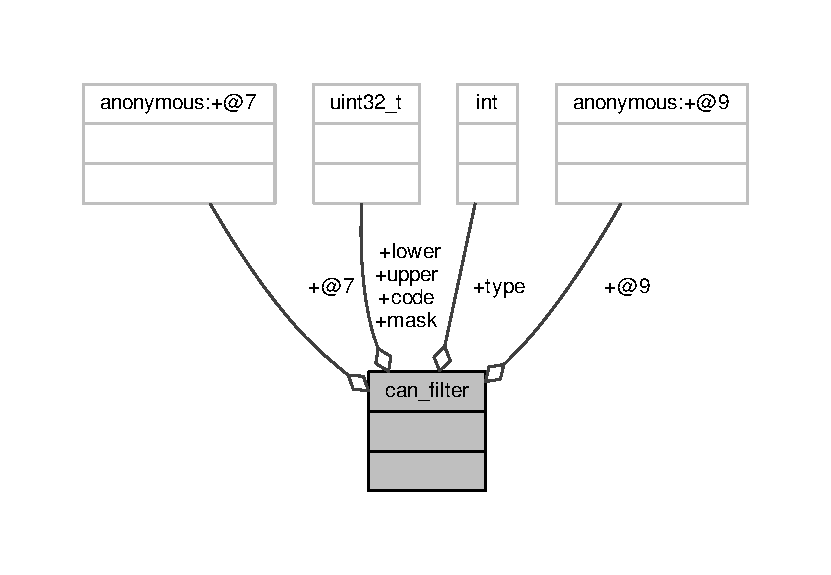
\includegraphics[width=350pt]{structcan__filter__coll__graph}
\end{center}
\end{figure}
\subsection*{Public Attributes}
\begin{DoxyCompactItemize}
\item 
int \hyperlink{structcan__filter_a796cdd0845b3b22c44028a898938d3e0}{type}
\item 
\begin{tabbing}
xx\=xx\=xx\=xx\=xx\=xx\=xx\=xx\=xx\=\kill
union \{\\
\>uint32\_t \hyperlink{structcan__filter_a15632117f3f031fbbeb28ef562f9ac94}{mask}\\
\>uint32\_t \hyperlink{structcan__filter_a75039f47394150965764154e50f2f3e1}{upper}\\
\}; \\

\end{tabbing}\item 
\begin{tabbing}
xx\=xx\=xx\=xx\=xx\=xx\=xx\=xx\=xx\=\kill
union \{\\
\>uint32\_t \hyperlink{structcan__filter_a33aa98b8a3e04907890496958dcf63da}{code}\\
\>uint32\_t \hyperlink{structcan__filter_aeb05b2987bb06a96739257032fbeaacd}{lower}\\
\}; \\

\end{tabbing}\end{DoxyCompactItemize}


\subsection{Member Data Documentation}
\subsubsection[{\texorpdfstring{"@7}{@7}}]{\setlength{\rightskip}{0pt plus 5cm}union \{ ... \} }\hypertarget{structcan__filter_a4831e5deb6d6475d8cad3ceae529c51f}{}\label{structcan__filter_a4831e5deb6d6475d8cad3ceae529c51f}
\subsubsection[{\texorpdfstring{"@9}{@9}}]{\setlength{\rightskip}{0pt plus 5cm}union \{ ... \} }\hypertarget{structcan__filter_afbb39bd7340f5fa3ce79d138919840d8}{}\label{structcan__filter_afbb39bd7340f5fa3ce79d138919840d8}
\index{can\+\_\+filter@{can\+\_\+filter}!code@{code}}
\index{code@{code}!can\+\_\+filter@{can\+\_\+filter}}
\subsubsection[{\texorpdfstring{code}{code}}]{\setlength{\rightskip}{0pt plus 5cm}uint32\+\_\+t can\+\_\+filter\+::code}\hypertarget{structcan__filter_a33aa98b8a3e04907890496958dcf63da}{}\label{structcan__filter_a33aa98b8a3e04907890496958dcf63da}
\index{can\+\_\+filter@{can\+\_\+filter}!lower@{lower}}
\index{lower@{lower}!can\+\_\+filter@{can\+\_\+filter}}
\subsubsection[{\texorpdfstring{lower}{lower}}]{\setlength{\rightskip}{0pt plus 5cm}uint32\+\_\+t can\+\_\+filter\+::lower}\hypertarget{structcan__filter_aeb05b2987bb06a96739257032fbeaacd}{}\label{structcan__filter_aeb05b2987bb06a96739257032fbeaacd}
\index{can\+\_\+filter@{can\+\_\+filter}!mask@{mask}}
\index{mask@{mask}!can\+\_\+filter@{can\+\_\+filter}}
\subsubsection[{\texorpdfstring{mask}{mask}}]{\setlength{\rightskip}{0pt plus 5cm}uint32\+\_\+t can\+\_\+filter\+::mask}\hypertarget{structcan__filter_a15632117f3f031fbbeb28ef562f9ac94}{}\label{structcan__filter_a15632117f3f031fbbeb28ef562f9ac94}
\index{can\+\_\+filter@{can\+\_\+filter}!type@{type}}
\index{type@{type}!can\+\_\+filter@{can\+\_\+filter}}
\subsubsection[{\texorpdfstring{type}{type}}]{\setlength{\rightskip}{0pt plus 5cm}int can\+\_\+filter\+::type}\hypertarget{structcan__filter_a796cdd0845b3b22c44028a898938d3e0}{}\label{structcan__filter_a796cdd0845b3b22c44028a898938d3e0}
\index{can\+\_\+filter@{can\+\_\+filter}!upper@{upper}}
\index{upper@{upper}!can\+\_\+filter@{can\+\_\+filter}}
\subsubsection[{\texorpdfstring{upper}{upper}}]{\setlength{\rightskip}{0pt plus 5cm}uint32\+\_\+t can\+\_\+filter\+::upper}\hypertarget{structcan__filter_a75039f47394150965764154e50f2f3e1}{}\label{structcan__filter_a75039f47394150965764154e50f2f3e1}


The documentation for this struct was generated from the following file\+:\begin{DoxyCompactItemize}
\item 
\hyperlink{hico__api_8h}{hico\+\_\+api.\+h}\end{DoxyCompactItemize}

\hypertarget{structcan__msg}{}\section{can\+\_\+msg Struct Reference}
\label{structcan__msg}\index{can\+\_\+msg@{can\+\_\+msg}}


{\ttfamily \#include $<$candatatypes.\+h$>$}



Collaboration diagram for can\+\_\+msg\+:\nopagebreak
\begin{figure}[H]
\begin{center}
\leavevmode
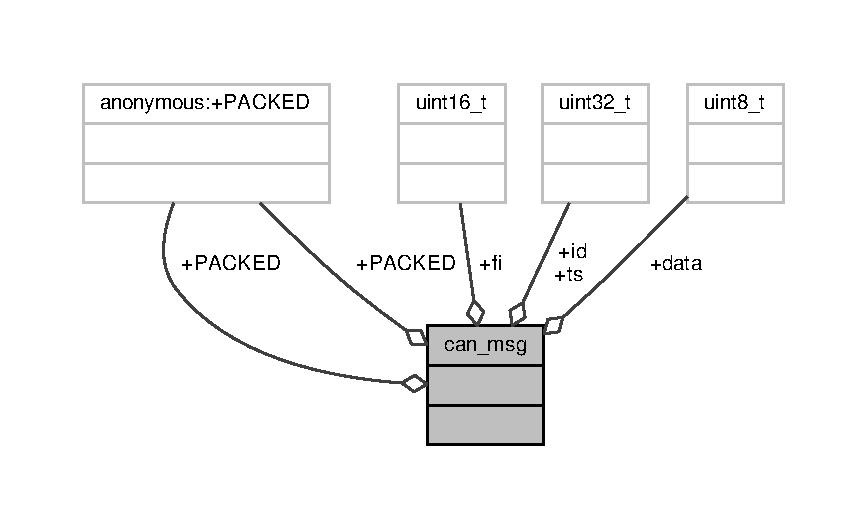
\includegraphics[width=350pt]{structcan__msg__coll__graph}
\end{center}
\end{figure}
\subsection*{Public Attributes}
\begin{DoxyCompactItemize}
\item 
\begin{tabbing}
xx\=xx\=xx\=xx\=xx\=xx\=xx\=xx\=xx\=\kill
union \{\\
\>uint16\_t \hyperlink{structcan__msg_ad1e9cccb168fbc295bb79ef7d9c5c915}{fi}\\
\} \hyperlink{structcan__msg_a233f7f010cc90ec3d453bcb75d66c14e}{PACKED}\\

\end{tabbing}\item 
uint32\+\_\+t \hyperlink{structcan__msg_a157aaad2daf039f59606522c6a51663a}{ts}
\item 
uint32\+\_\+t \hyperlink{structcan__msg_a9a5f820883d3dfe1f0c6bc33c3f95989}{id}
\item 
uint8\+\_\+t \hyperlink{structcan__msg_ac0dab268ebadaa9521b4d535c03f13d8}{data} \mbox{[}8\mbox{]}
\item 
\begin{tabbing}
xx\=xx\=xx\=xx\=xx\=xx\=xx\=xx\=xx\=\kill
union \{\\
\>uint16\_t \hyperlink{structcan__msg_ad1e9cccb168fbc295bb79ef7d9c5c915}{fi}\\
\} \hyperlink{structcan__msg_a11a48cac095afd9250fe22fa37929aec}{PACKED}\\

\end{tabbing}\end{DoxyCompactItemize}


\subsection{Member Data Documentation}
\index{can\+\_\+msg@{can\+\_\+msg}!data@{data}}
\index{data@{data}!can\+\_\+msg@{can\+\_\+msg}}
\subsubsection[{\texorpdfstring{data}{data}}]{\setlength{\rightskip}{0pt plus 5cm}uint8\+\_\+t can\+\_\+msg\+::data}\hypertarget{structcan__msg_ac0dab268ebadaa9521b4d535c03f13d8}{}\label{structcan__msg_ac0dab268ebadaa9521b4d535c03f13d8}
\index{can\+\_\+msg@{can\+\_\+msg}!fi@{fi}}
\index{fi@{fi}!can\+\_\+msg@{can\+\_\+msg}}
\subsubsection[{\texorpdfstring{fi}{fi}}]{\setlength{\rightskip}{0pt plus 5cm}uint16\+\_\+t can\+\_\+msg\+::fi}\hypertarget{structcan__msg_ad1e9cccb168fbc295bb79ef7d9c5c915}{}\label{structcan__msg_ad1e9cccb168fbc295bb79ef7d9c5c915}
\index{can\+\_\+msg@{can\+\_\+msg}!id@{id}}
\index{id@{id}!can\+\_\+msg@{can\+\_\+msg}}
\subsubsection[{\texorpdfstring{id}{id}}]{\setlength{\rightskip}{0pt plus 5cm}uint32\+\_\+t can\+\_\+msg\+::id}\hypertarget{structcan__msg_a9a5f820883d3dfe1f0c6bc33c3f95989}{}\label{structcan__msg_a9a5f820883d3dfe1f0c6bc33c3f95989}
\index{can\+\_\+msg@{can\+\_\+msg}!P\+A\+C\+K\+ED@{P\+A\+C\+K\+ED}}
\index{P\+A\+C\+K\+ED@{P\+A\+C\+K\+ED}!can\+\_\+msg@{can\+\_\+msg}}
\subsubsection[{\texorpdfstring{P\+A\+C\+K\+ED}{PACKED}}]{\setlength{\rightskip}{0pt plus 5cm}union \{ ... \}  can\+\_\+msg\+::\+P\+A\+C\+K\+ED}\hypertarget{structcan__msg_a233f7f010cc90ec3d453bcb75d66c14e}{}\label{structcan__msg_a233f7f010cc90ec3d453bcb75d66c14e}
\index{can\+\_\+msg@{can\+\_\+msg}!P\+A\+C\+K\+ED@{P\+A\+C\+K\+ED}}
\index{P\+A\+C\+K\+ED@{P\+A\+C\+K\+ED}!can\+\_\+msg@{can\+\_\+msg}}
\subsubsection[{\texorpdfstring{P\+A\+C\+K\+ED}{PACKED}}]{\setlength{\rightskip}{0pt plus 5cm}union \{ ... \}  can\+\_\+msg\+::\+P\+A\+C\+K\+ED}\hypertarget{structcan__msg_a11a48cac095afd9250fe22fa37929aec}{}\label{structcan__msg_a11a48cac095afd9250fe22fa37929aec}
\index{can\+\_\+msg@{can\+\_\+msg}!ts@{ts}}
\index{ts@{ts}!can\+\_\+msg@{can\+\_\+msg}}
\subsubsection[{\texorpdfstring{ts}{ts}}]{\setlength{\rightskip}{0pt plus 5cm}uint32\+\_\+t can\+\_\+msg\+::ts}\hypertarget{structcan__msg_a157aaad2daf039f59606522c6a51663a}{}\label{structcan__msg_a157aaad2daf039f59606522c6a51663a}


The documentation for this struct was generated from the following files\+:\begin{DoxyCompactItemize}
\item 
\hyperlink{candatatypes_8h}{candatatypes.\+h}\item 
\hyperlink{hico__api_8h}{hico\+\_\+api.\+h}\end{DoxyCompactItemize}

\hypertarget{classCanBusPort}{}\section{Can\+Bus\+Port Class Reference}
\label{classCanBusPort}\index{Can\+Bus\+Port@{Can\+Bus\+Port}}


{\ttfamily \#include $<$Can\+Bus\+Port.\+h$>$}



Inheritance diagram for Can\+Bus\+Port\+:
\nopagebreak
\begin{figure}[H]
\begin{center}
\leavevmode
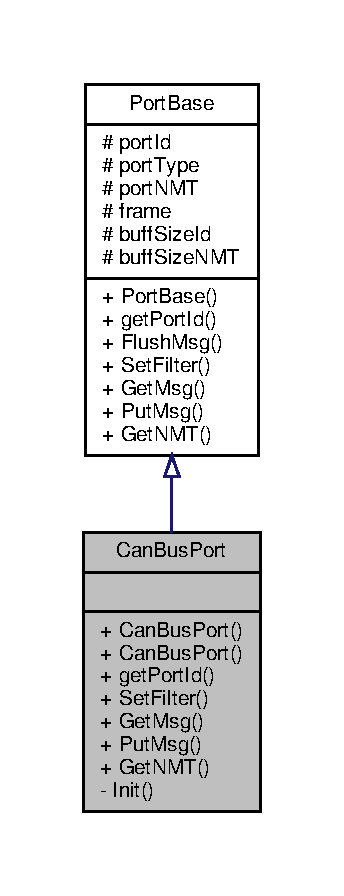
\includegraphics[width=165pt]{classCanBusPort__inherit__graph}
\end{center}
\end{figure}


Collaboration diagram for Can\+Bus\+Port\+:
\nopagebreak
\begin{figure}[H]
\begin{center}
\leavevmode
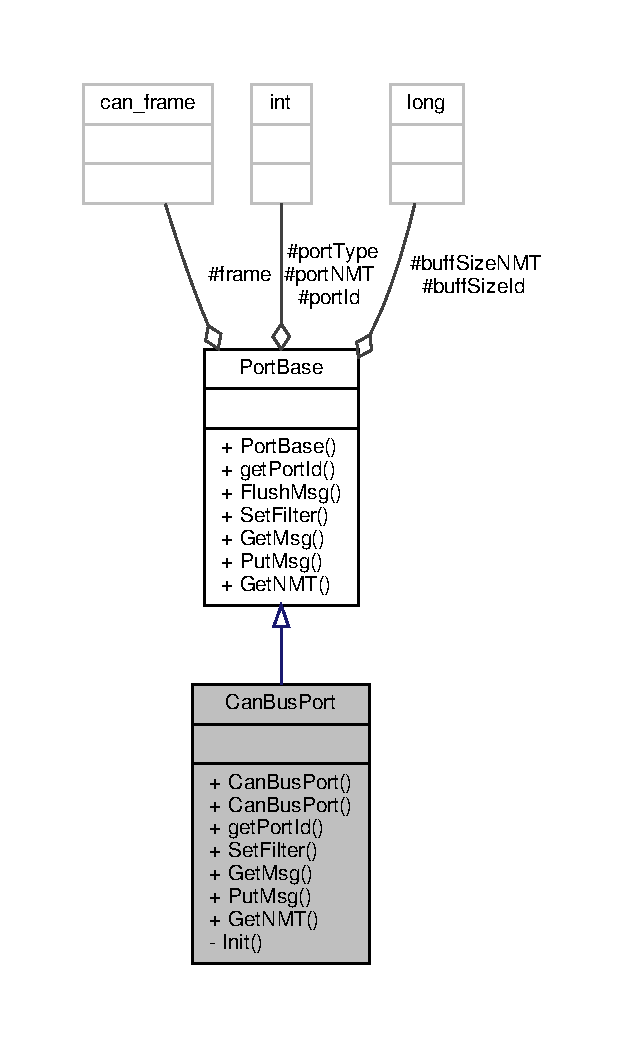
\includegraphics[width=301pt]{classCanBusPort__coll__graph}
\end{center}
\end{figure}
\subsection*{Public Member Functions}
\begin{DoxyCompactItemize}
\item 
\hyperlink{classCanBusPort_a4ccb8d39da6185bfe5c1dee38db51987}{Can\+Bus\+Port} ()
\begin{DoxyCompactList}\small\item\em \hyperlink{classCanBusPort}{Can\+Bus\+Port}\+: Empty constructor. Initialize default port \char`\"{}/dev/can0\char`\"{}. \end{DoxyCompactList}\item 
\hyperlink{classCanBusPort_ad4649a2da594bbffc267483646fb1405}{Can\+Bus\+Port} (string can\+Port)
\begin{DoxyCompactList}\small\item\em \hyperlink{classCanBusPort}{Can\+Bus\+Port}\+: Initialization of one port given a device name. \end{DoxyCompactList}\item 
int \hyperlink{classCanBusPort_a7c6b733c5834d4ab3e1906d847a2234a}{get\+Port\+Id} ()
\item 
long \hyperlink{classCanBusPort_af09c794e3af86e89c8a511535f856dc9}{Set\+Filter} (uint32\+\_\+t can\+Id, uint32\+\_\+t mask)
\item 
long \hyperlink{classCanBusPort_ac442e4e5b7bb154ea6322518b715f406}{Get\+Msg} (uint32\+\_\+t \&can\+Id, uint8\+\_\+t $\ast$data, uint8\+\_\+t \&size)
\item 
long \hyperlink{classCanBusPort_a2bb802ad7a14e260f0f51b79d4c53c43}{Put\+Msg} (const uint32\+\_\+t \&can\+Id, uint8\+\_\+t $\ast$const data, const uint8\+\_\+t size)
\item 
long \hyperlink{classCanBusPort_a41242dc7980ca398e4770813e50ef32b}{Get\+N\+MT} (uint8\+\_\+t $\ast$const data, uint8\+\_\+t \&size)
\end{DoxyCompactItemize}
\subsection*{Private Member Functions}
\begin{DoxyCompactItemize}
\item 
long \hyperlink{classCanBusPort_a0de0778cfc475d2da559668be55f6015}{Init} (string can\+Port)
\end{DoxyCompactItemize}
\subsection*{Additional Inherited Members}


\subsection{Constructor \& Destructor Documentation}
\index{Can\+Bus\+Port@{Can\+Bus\+Port}!Can\+Bus\+Port@{Can\+Bus\+Port}}
\index{Can\+Bus\+Port@{Can\+Bus\+Port}!Can\+Bus\+Port@{Can\+Bus\+Port}}
\subsubsection[{\texorpdfstring{Can\+Bus\+Port()}{CanBusPort()}}]{\setlength{\rightskip}{0pt plus 5cm}Can\+Bus\+Port\+::\+Can\+Bus\+Port (
\begin{DoxyParamCaption}
{}
\end{DoxyParamCaption}
)}\hypertarget{classCanBusPort_a4ccb8d39da6185bfe5c1dee38db51987}{}\label{classCanBusPort_a4ccb8d39da6185bfe5c1dee38db51987}


\hyperlink{classCanBusPort}{Can\+Bus\+Port}\+: Empty constructor. Initialize default port \char`\"{}/dev/can0\char`\"{}. 

\index{Can\+Bus\+Port@{Can\+Bus\+Port}!Can\+Bus\+Port@{Can\+Bus\+Port}}
\index{Can\+Bus\+Port@{Can\+Bus\+Port}!Can\+Bus\+Port@{Can\+Bus\+Port}}
\subsubsection[{\texorpdfstring{Can\+Bus\+Port(string can\+Port)}{CanBusPort(string canPort)}}]{\setlength{\rightskip}{0pt plus 5cm}Can\+Bus\+Port\+::\+Can\+Bus\+Port (
\begin{DoxyParamCaption}
\item[{string}]{can\+Port}
\end{DoxyParamCaption}
)}\hypertarget{classCanBusPort_ad4649a2da594bbffc267483646fb1405}{}\label{classCanBusPort_ad4649a2da594bbffc267483646fb1405}


\hyperlink{classCanBusPort}{Can\+Bus\+Port}\+: Initialization of one port given a device name. 


\begin{DoxyParams}{Parameters}
{\em can\+Port} & String with the name of system device. \\
\hline
\end{DoxyParams}


\subsection{Member Function Documentation}
\index{Can\+Bus\+Port@{Can\+Bus\+Port}!Get\+Msg@{Get\+Msg}}
\index{Get\+Msg@{Get\+Msg}!Can\+Bus\+Port@{Can\+Bus\+Port}}
\subsubsection[{\texorpdfstring{Get\+Msg(uint32\+\_\+t \&can\+Id, uint8\+\_\+t $\ast$data, uint8\+\_\+t \&size)}{GetMsg(uint32_t &canId, uint8_t *data, uint8_t &size)}}]{\setlength{\rightskip}{0pt plus 5cm}long Can\+Bus\+Port\+::\+Get\+Msg (
\begin{DoxyParamCaption}
\item[{uint32\+\_\+t \&}]{can\+Id, }
\item[{uint8\+\_\+t $\ast$}]{data, }
\item[{uint8\+\_\+t \&}]{size}
\end{DoxyParamCaption}
)\hspace{0.3cm}{\ttfamily [virtual]}}\hypertarget{classCanBusPort_ac442e4e5b7bb154ea6322518b715f406}{}\label{classCanBusPort_ac442e4e5b7bb154ea6322518b715f406}


Implements \hyperlink{classPortBase_a4fe82768f2b79889d7084292ac0e8696}{Port\+Base}.

\index{Can\+Bus\+Port@{Can\+Bus\+Port}!Get\+N\+MT@{Get\+N\+MT}}
\index{Get\+N\+MT@{Get\+N\+MT}!Can\+Bus\+Port@{Can\+Bus\+Port}}
\subsubsection[{\texorpdfstring{Get\+N\+M\+T(uint8\+\_\+t $\ast$const data, uint8\+\_\+t \&size)}{GetNMT(uint8_t *const data, uint8_t &size)}}]{\setlength{\rightskip}{0pt plus 5cm}long Can\+Bus\+Port\+::\+Get\+N\+MT (
\begin{DoxyParamCaption}
\item[{uint8\+\_\+t $\ast$const}]{data, }
\item[{uint8\+\_\+t \&}]{size}
\end{DoxyParamCaption}
)\hspace{0.3cm}{\ttfamily [virtual]}}\hypertarget{classCanBusPort_a41242dc7980ca398e4770813e50ef32b}{}\label{classCanBusPort_a41242dc7980ca398e4770813e50ef32b}


Implements \hyperlink{classPortBase_abab2bf17b01d87c2bca01cb2151aa2f1}{Port\+Base}.

\index{Can\+Bus\+Port@{Can\+Bus\+Port}!get\+Port\+Id@{get\+Port\+Id}}
\index{get\+Port\+Id@{get\+Port\+Id}!Can\+Bus\+Port@{Can\+Bus\+Port}}
\subsubsection[{\texorpdfstring{get\+Port\+Id()}{getPortId()}}]{\setlength{\rightskip}{0pt plus 5cm}int Can\+Bus\+Port\+::get\+Port\+Id (
\begin{DoxyParamCaption}
{}
\end{DoxyParamCaption}
)}\hypertarget{classCanBusPort_a7c6b733c5834d4ab3e1906d847a2234a}{}\label{classCanBusPort_a7c6b733c5834d4ab3e1906d847a2234a}
\index{Can\+Bus\+Port@{Can\+Bus\+Port}!Init@{Init}}
\index{Init@{Init}!Can\+Bus\+Port@{Can\+Bus\+Port}}
\subsubsection[{\texorpdfstring{Init(string can\+Port)}{Init(string canPort)}}]{\setlength{\rightskip}{0pt plus 5cm}long Can\+Bus\+Port\+::\+Init (
\begin{DoxyParamCaption}
\item[{string}]{can\+Port}
\end{DoxyParamCaption}
)\hspace{0.3cm}{\ttfamily [private]}}\hypertarget{classCanBusPort_a0de0778cfc475d2da559668be55f6015}{}\label{classCanBusPort_a0de0778cfc475d2da559668be55f6015}
\index{Can\+Bus\+Port@{Can\+Bus\+Port}!Put\+Msg@{Put\+Msg}}
\index{Put\+Msg@{Put\+Msg}!Can\+Bus\+Port@{Can\+Bus\+Port}}
\subsubsection[{\texorpdfstring{Put\+Msg(const uint32\+\_\+t \&can\+Id, uint8\+\_\+t $\ast$const data, const uint8\+\_\+t size)}{PutMsg(const uint32_t &canId, uint8_t *const data, const uint8_t size)}}]{\setlength{\rightskip}{0pt plus 5cm}long Can\+Bus\+Port\+::\+Put\+Msg (
\begin{DoxyParamCaption}
\item[{const uint32\+\_\+t \&}]{can\+Id, }
\item[{uint8\+\_\+t $\ast$const}]{data, }
\item[{const uint8\+\_\+t}]{size}
\end{DoxyParamCaption}
)\hspace{0.3cm}{\ttfamily [virtual]}}\hypertarget{classCanBusPort_a2bb802ad7a14e260f0f51b79d4c53c43}{}\label{classCanBusPort_a2bb802ad7a14e260f0f51b79d4c53c43}


Implements \hyperlink{classPortBase_a26213ebb6ea0a0b77f60c28944e3bb8e}{Port\+Base}.

\index{Can\+Bus\+Port@{Can\+Bus\+Port}!Set\+Filter@{Set\+Filter}}
\index{Set\+Filter@{Set\+Filter}!Can\+Bus\+Port@{Can\+Bus\+Port}}
\subsubsection[{\texorpdfstring{Set\+Filter(uint32\+\_\+t can\+Id, uint32\+\_\+t mask)}{SetFilter(uint32_t canId, uint32_t mask)}}]{\setlength{\rightskip}{0pt plus 5cm}long Can\+Bus\+Port\+::\+Set\+Filter (
\begin{DoxyParamCaption}
\item[{uint32\+\_\+t}]{can\+Id, }
\item[{uint32\+\_\+t}]{mask}
\end{DoxyParamCaption}
)\hspace{0.3cm}{\ttfamily [virtual]}}\hypertarget{classCanBusPort_af09c794e3af86e89c8a511535f856dc9}{}\label{classCanBusPort_af09c794e3af86e89c8a511535f856dc9}


Implements \hyperlink{classPortBase_a1d857a81a8e3f3bd460ef7c802ee762c}{Port\+Base}.



The documentation for this class was generated from the following files\+:\begin{DoxyCompactItemize}
\item 
\hyperlink{CanBusPort_8h}{Can\+Bus\+Port.\+h}\item 
\hyperlink{CanBusPort_8cpp}{Can\+Bus\+Port.\+cpp}\end{DoxyCompactItemize}

\hypertarget{classCiA301CommPort}{}\section{Ci\+A301\+Comm\+Port Class Reference}
\label{classCiA301CommPort}\index{Ci\+A301\+Comm\+Port@{Ci\+A301\+Comm\+Port}}


{\ttfamily \#include $<$Ci\+A301\+Comm\+Port.\+h$>$}



Inheritance diagram for Ci\+A301\+Comm\+Port\+:
\nopagebreak
\begin{figure}[H]
\begin{center}
\leavevmode
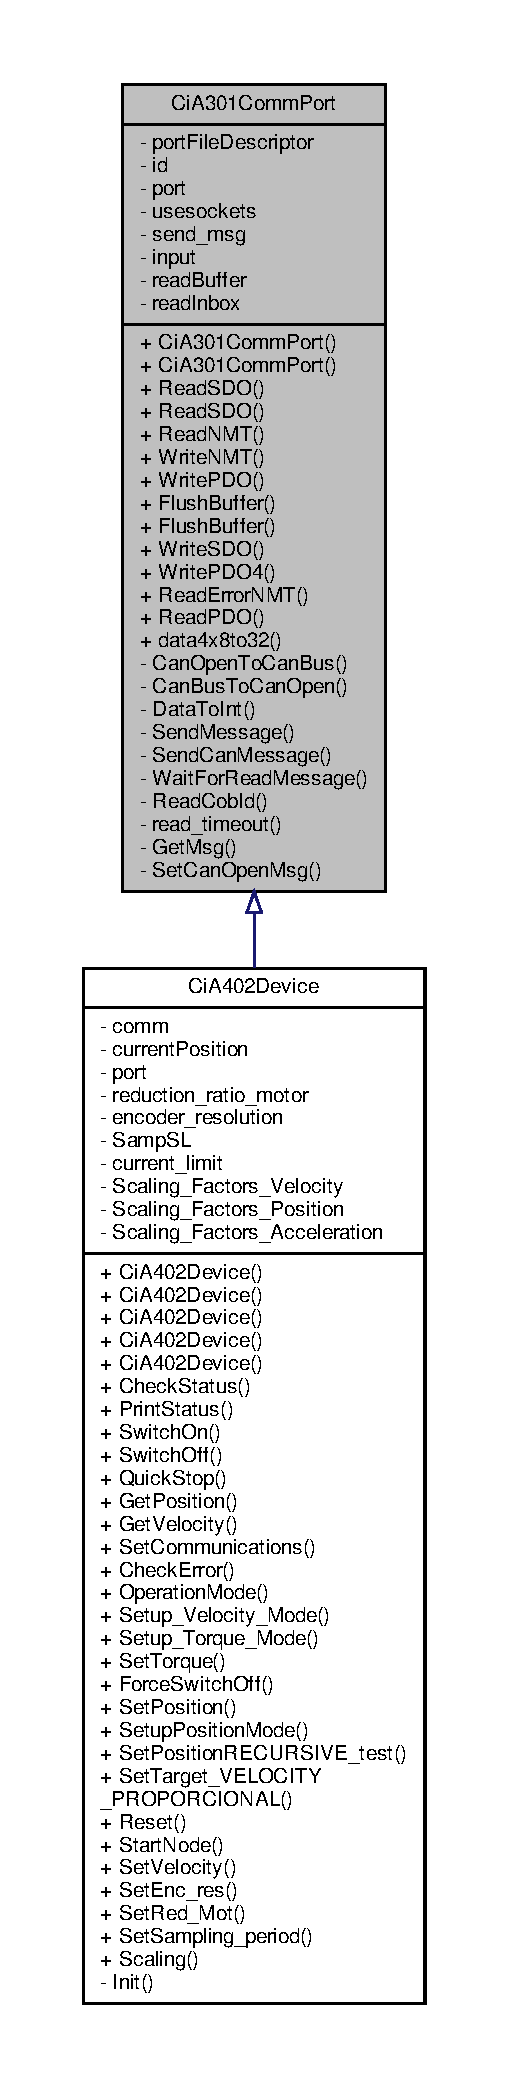
\includegraphics[height=550pt]{classCiA301CommPort__inherit__graph}
\end{center}
\end{figure}


Collaboration diagram for Ci\+A301\+Comm\+Port\+:
\nopagebreak
\begin{figure}[H]
\begin{center}
\leavevmode
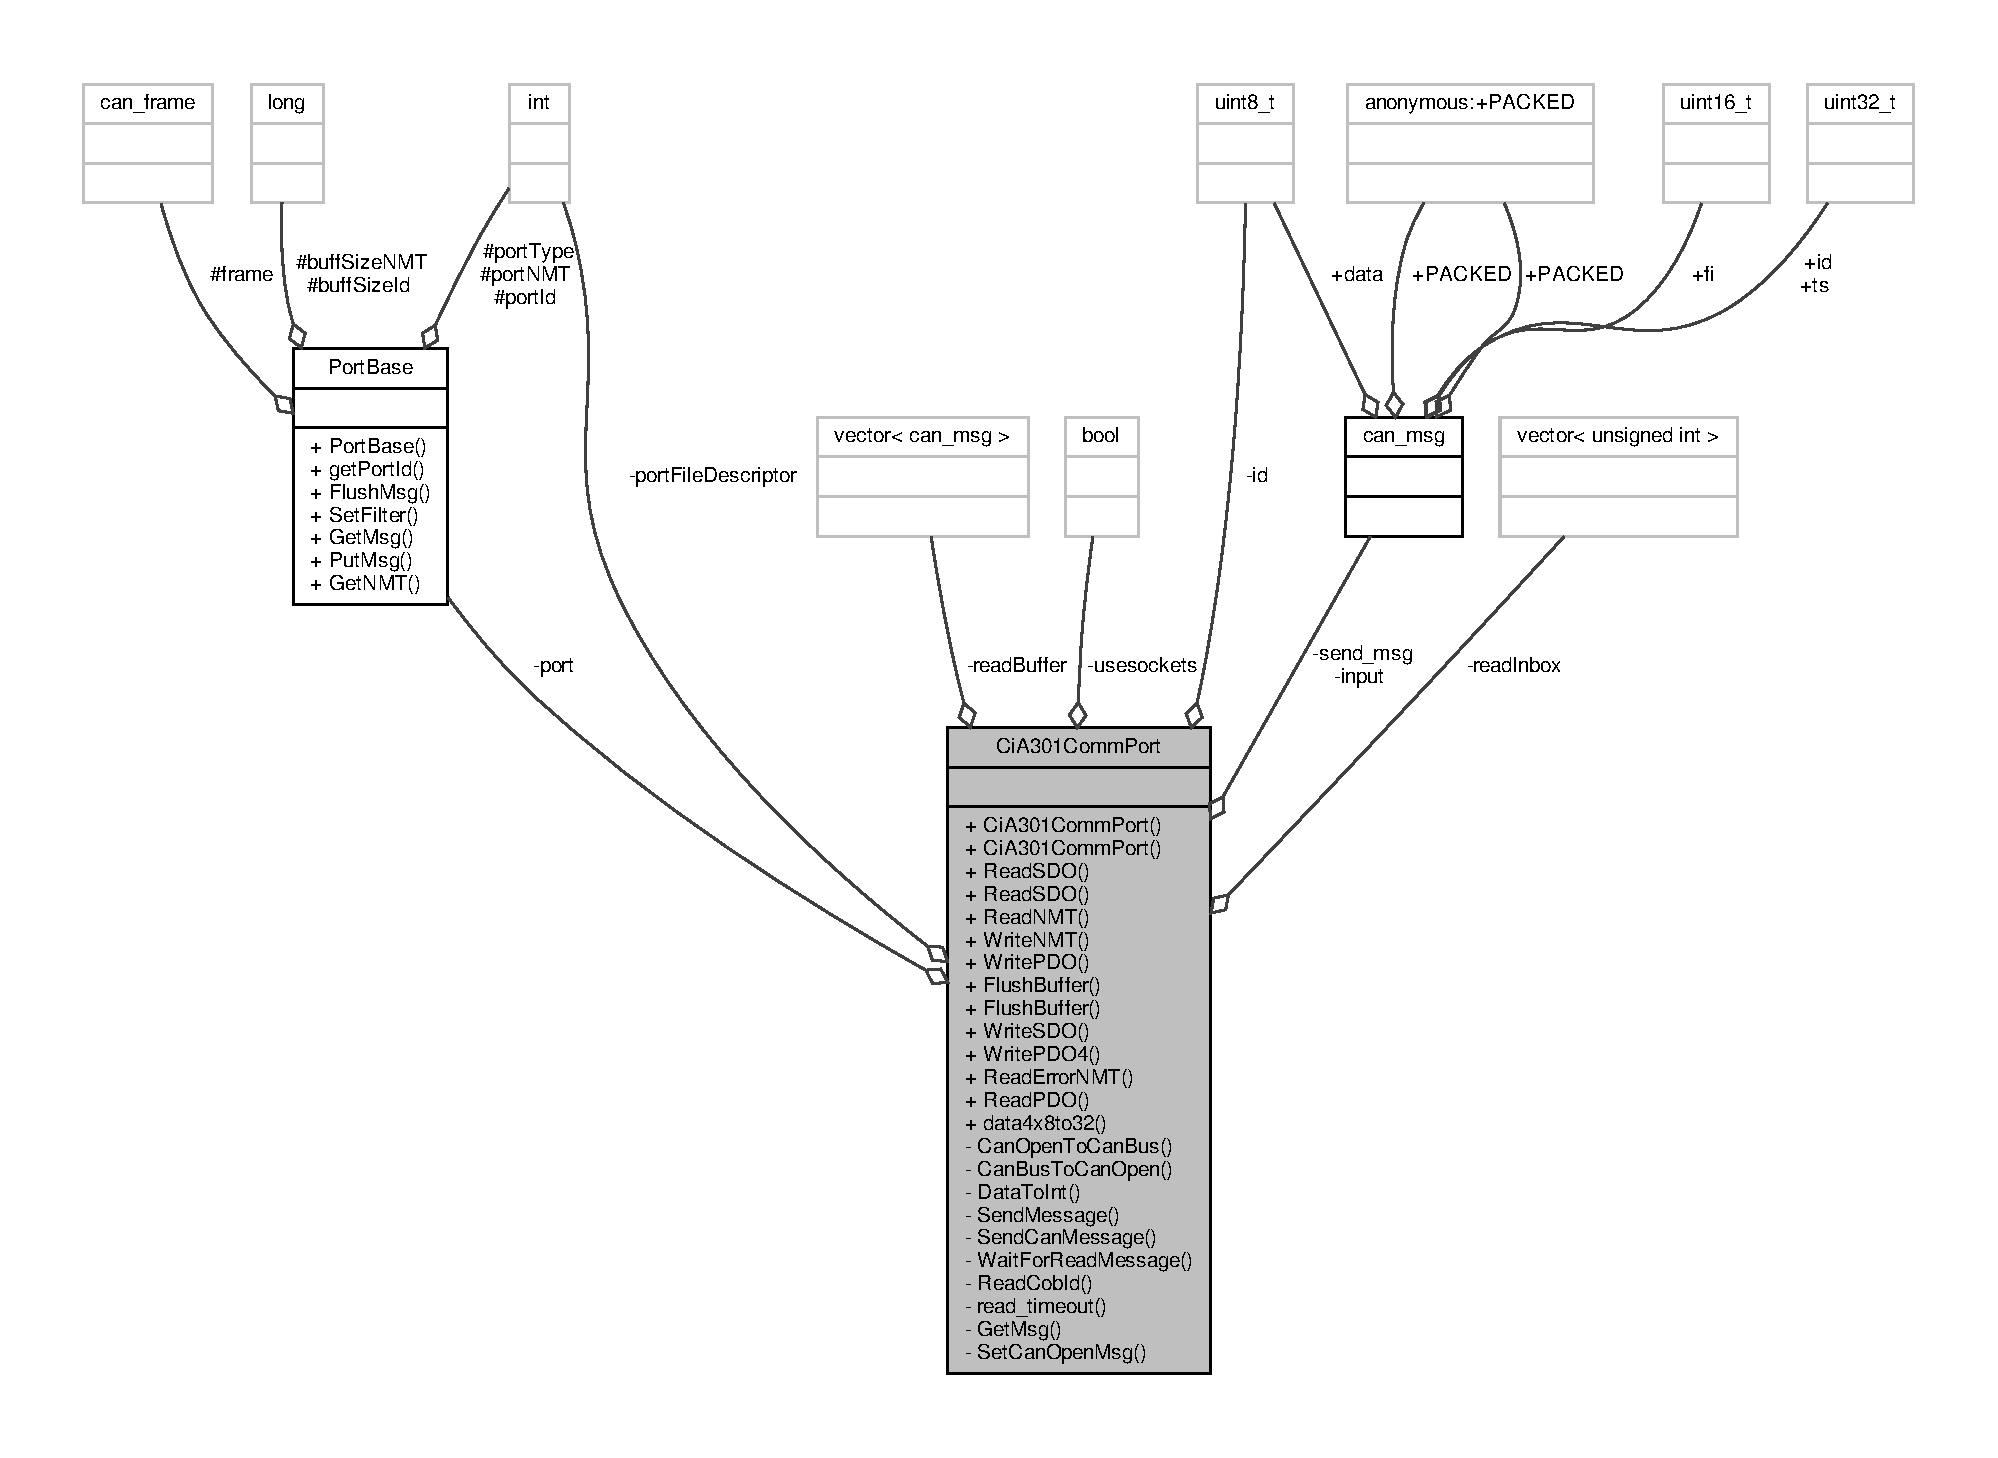
\includegraphics[width=350pt]{classCiA301CommPort__coll__graph}
\end{center}
\end{figure}
\subsection*{Public Member Functions}
\begin{DoxyCompactItemize}
\item 
\hyperlink{classCiA301CommPort_aae705cb5c6a405ef74a10e5220d0b08f}{Ci\+A301\+Comm\+Port} (int new\+Port\+File\+Descriptor, uint8\+\_\+t new\+\_\+id)
\item 
\hyperlink{classCiA301CommPort_a1e05c4b292cfee36ff9eeddb2c8eb4c0}{Ci\+A301\+Comm\+Port} (\hyperlink{classPortBase}{Port\+Base} $\ast$new\+\_\+port, uint8\+\_\+t new\+\_\+id)
\item 
long \hyperlink{classCiA301CommPort_a0fd0920052684589bc37bb898dcdd758}{Read\+S\+DO} (vector$<$ uint8\+\_\+t $>$ address, int subindex)
\item 
ulong \hyperlink{classCiA301CommPort_a403c1de504a2a5c36c90dd977e1bd536}{Read\+S\+DO} (const vector$<$ uint8\+\_\+t $>$ \&address)
\begin{DoxyCompactList}\small\item\em \hyperlink{classCiA301CommPort_a0fd0920052684589bc37bb898dcdd758}{Ci\+A301\+Comm\+Port\+::\+Read\+S\+DO} Waits until expected. \end{DoxyCompactList}\item 
long \hyperlink{classCiA301CommPort_a02df85ed5140d0d7a57fe0d2f6e47ea1}{Read\+N\+MT} (const vector$<$ uint8\+\_\+t $>$ \&nmt\+Code)
\item 
long \hyperlink{classCiA301CommPort_a09feb3f78831c9fbb683a85cc3bc4562}{Write\+N\+MT} (const vector$<$ uint8\+\_\+t $>$ \&nmt\+Command)
\begin{DoxyCompactList}\small\item\em Write\+N\+MT This function sends N\+MT message from node to Can\+Bus. \end{DoxyCompactList}\item 
long \hyperlink{classCiA301CommPort_a56d2c604b11363e6b287f59b68a546bd}{Write\+P\+DO} (const vector$<$ uint8\+\_\+t $>$ \&command)
\begin{DoxyCompactList}\small\item\em Write\+P\+DO This function sends P\+DO message to a node (the mode id is configured on constructor). \end{DoxyCompactList}\item 
long \hyperlink{classCiA301CommPort_a067cddaf01932fa6fa27255c61b08190}{Flush\+Buffer} ()
\item 
long \hyperlink{classCiA301CommPort_ab29e221039a2d21d1446edb09b91864e}{Flush\+Buffer} (int msgs)
\begin{DoxyCompactList}\small\item\em Flush\+Buffer Removes the msgs number of can frames from buffer. \end{DoxyCompactList}\item 
long \hyperlink{classCiA301CommPort_a4d97c27423b2323f8475f6e5c2f91575}{Write\+S\+DO} (const vector$<$ uint8\+\_\+t $>$ \&address, const vector$<$ uint8\+\_\+t $>$ \&value)
\begin{DoxyCompactList}\small\item\em Write\+S\+DO Writes 4 byte value to specific address on device. This function sends S\+DO message requesting write on the object dictionary address. Also block and wait for the S\+DO msg for write ack, and returns negative if error. As it reads the ack S\+DO message, the buffer should be same size after this function returns. \end{DoxyCompactList}\item 
long \hyperlink{classCiA301CommPort_a1faf4f37530e0dd0ae4600cfb0b1d742}{Write\+P\+D\+O4} (const vector$<$ uint8\+\_\+t $>$ \&command)
\item 
long \hyperlink{classCiA301CommPort_a46534ff9e7e2a05a0b4913e4331710e5}{Read\+Error\+N\+MT} ()
\item 
long \hyperlink{classCiA301CommPort_a827f3e594b9f1e57a7b7ccb8a278404a}{Read\+P\+DO} (long number)
\item 
uint32\+\_\+t \hyperlink{classCiA301CommPort_a2e85303159577f6b3209b741e9871cc5}{data4x8to32} (const uint8\+\_\+t $\ast$in, int dlc)
\end{DoxyCompactItemize}
\subsection*{Private Member Functions}
\begin{DoxyCompactItemize}
\item 
long \hyperlink{classCiA301CommPort_a26346f83700bc8403a315be01c6508e0}{Can\+Open\+To\+Can\+Bus} (const \hyperlink{structco__msg}{co\+\_\+msg} \&\hyperlink{classCiA301CommPort_ae0f955c7141e2067307cea0b48e111d4}{input}, \hyperlink{structcan__msg}{can\+\_\+msg} \&output)
\begin{DoxyCompactList}\small\item\em Can\+Open\+To\+Can\+Bus\+: Converts a Can\+Open object or message into a Can\+Bus object or message. For this, it receives two parameters passed by reference, one of an object Can\+Open that will become the other Can\+Bus object. To do this, copy the ids, the dlc, the rtr, the ts, select the normal frame for the Can\+Bus message and finally copy the message information. \end{DoxyCompactList}\item 
long \hyperlink{classCiA301CommPort_aa16887712ea9cad534aacd4851f9190d}{Can\+Bus\+To\+Can\+Open} (const \hyperlink{structcan__msg}{can\+\_\+msg} \&\hyperlink{classCiA301CommPort_ae0f955c7141e2067307cea0b48e111d4}{input}, \hyperlink{structco__msg}{co\+\_\+msg} \&output)
\begin{DoxyCompactList}\small\item\em Can\+Bus\+To\+Can\+Open\+: It performs the inverse task to the previous function. This function converts a Can\+Bus object or message in another Can\+Open object or message both passed by reference. To do this, copy the information in the Can\+Open message Can\+Bus message data\+: the id, the dlc, the rtr, the ts and the data information which contains (the content of the message itself). \end{DoxyCompactList}\item 
ulong \hyperlink{classCiA301CommPort_a4e62245791e907b5df74e3612f8fc9ce}{Data\+To\+Int} (const uint8\+\_\+t $\ast$in, unsigned short size)
\item 
int \hyperlink{classCiA301CommPort_aeae04455e1e1a1ca1beed9478372c031}{Send\+Message} (\hyperlink{structco__msg}{co\+\_\+msg} \hyperlink{classCiA301CommPort_ae0f955c7141e2067307cea0b48e111d4}{input})
\item 
int \hyperlink{classCiA301CommPort_a700a04da67928ca50744617ece28cde5}{Send\+Can\+Message} (\hyperlink{structcan__msg}{can\+\_\+msg} \&\hyperlink{classCiA301CommPort_ae0f955c7141e2067307cea0b48e111d4}{input})
\item 
int \hyperlink{classCiA301CommPort_a02ba7069a0497e3497f3dfaec2879b54}{Wait\+For\+Read\+Message} (\hyperlink{structco__msg}{co\+\_\+msg} \&output, unsigned int can\+Index)
\item 
int \hyperlink{classCiA301CommPort_a408f53d13935a1916ca6f21d08ae135e}{Read\+Cob\+Id} (uint16\+\_\+t expected\+\_\+cobid, \hyperlink{structco__msg}{co\+\_\+msg} \&output)
\begin{DoxyCompactList}\small\item\em Ci\+A301\+Comm\+Port\+::\+Wait\+For\+Answer Read the port until expected canopen answer shows up in the port reads. \end{DoxyCompactList}\item 
int \hyperlink{classCiA301CommPort_ae62c2389b38a0e217aff7ca17a3d87b6}{read\+\_\+timeout} (int fd, \hyperlink{structcan__msg}{can\+\_\+msg} $\ast$buf, unsigned int timeout)
\item 
long \hyperlink{classCiA301CommPort_a645450ca09e07ea6da339923ceeec934}{Get\+Msg} (\hyperlink{structcan__msg}{can\+\_\+msg} \&msg)
\item 
\hyperlink{structco__msg}{co\+\_\+msg} \hyperlink{classCiA301CommPort_a2c197480112989df6bdb9ea89a649636}{Set\+Can\+Open\+Msg} (unsigned short id\+\_\+co, unsigned short rtr, vector$<$ uint8\+\_\+t $>$ co\+Data\+Frame)
\begin{DoxyCompactList}\small\item\em \hyperlink{classCiA301CommPort_a2c197480112989df6bdb9ea89a649636}{Ci\+A301\+Comm\+Port\+::\+Set\+Can\+Open\+Msg} \+: Constructs canopen message from parameters. \end{DoxyCompactList}\end{DoxyCompactItemize}
\subsection*{Private Attributes}
\begin{DoxyCompactItemize}
\item 
int \hyperlink{classCiA301CommPort_adc50c8d333b18fcb1b5c61ca69ea05c6}{port\+File\+Descriptor}
\item 
uint8\+\_\+t \hyperlink{classCiA301CommPort_a1ae075d22fc854da21a6e691bb029fc0}{id}
\item 
\hyperlink{classPortBase}{Port\+Base} $\ast$ \hyperlink{classCiA301CommPort_a6b8366387075c99ee980d2ca79c7b7fc}{port}
\item 
bool \hyperlink{classCiA301CommPort_a579e0de814111bde3bbe18cceb76ce64}{usesockets}
\item 
\hyperlink{structcan__msg}{can\+\_\+msg} \hyperlink{classCiA301CommPort_ade81ac897a5d851d946dd7a18245b75d}{send\+\_\+msg}
\item 
\hyperlink{structcan__msg}{can\+\_\+msg} \hyperlink{classCiA301CommPort_ae0f955c7141e2067307cea0b48e111d4}{input}
\item 
vector$<$ \hyperlink{structcan__msg}{can\+\_\+msg} $>$ \hyperlink{classCiA301CommPort_a8b904f3591ecfb99fd82271343727215}{read\+Buffer}
\item 
vector$<$ unsigned int $>$ \hyperlink{classCiA301CommPort_a41b2fcb24a27e5280417db03d8cdb399}{read\+Inbox}
\end{DoxyCompactItemize}


\subsection{Constructor \& Destructor Documentation}
\index{Ci\+A301\+Comm\+Port@{Ci\+A301\+Comm\+Port}!Ci\+A301\+Comm\+Port@{Ci\+A301\+Comm\+Port}}
\index{Ci\+A301\+Comm\+Port@{Ci\+A301\+Comm\+Port}!Ci\+A301\+Comm\+Port@{Ci\+A301\+Comm\+Port}}
\subsubsection[{\texorpdfstring{Ci\+A301\+Comm\+Port(int new\+Port\+File\+Descriptor, uint8\+\_\+t new\+\_\+id)}{CiA301CommPort(int newPortFileDescriptor, uint8_t new_id)}}]{\setlength{\rightskip}{0pt plus 5cm}Ci\+A301\+Comm\+Port\+::\+Ci\+A301\+Comm\+Port (
\begin{DoxyParamCaption}
\item[{int}]{new\+Port\+File\+Descriptor, }
\item[{uint8\+\_\+t}]{new\+\_\+id}
\end{DoxyParamCaption}
)}\hypertarget{classCiA301CommPort_aae705cb5c6a405ef74a10e5220d0b08f}{}\label{classCiA301CommPort_aae705cb5c6a405ef74a10e5220d0b08f}
\index{Ci\+A301\+Comm\+Port@{Ci\+A301\+Comm\+Port}!Ci\+A301\+Comm\+Port@{Ci\+A301\+Comm\+Port}}
\index{Ci\+A301\+Comm\+Port@{Ci\+A301\+Comm\+Port}!Ci\+A301\+Comm\+Port@{Ci\+A301\+Comm\+Port}}
\subsubsection[{\texorpdfstring{Ci\+A301\+Comm\+Port(\+Port\+Base $\ast$new\+\_\+port, uint8\+\_\+t new\+\_\+id)}{CiA301CommPort(PortBase *new_port, uint8_t new_id)}}]{\setlength{\rightskip}{0pt plus 5cm}Ci\+A301\+Comm\+Port\+::\+Ci\+A301\+Comm\+Port (
\begin{DoxyParamCaption}
\item[{{\bf Port\+Base} $\ast$}]{new\+\_\+port, }
\item[{uint8\+\_\+t}]{new\+\_\+id}
\end{DoxyParamCaption}
)}\hypertarget{classCiA301CommPort_a1e05c4b292cfee36ff9eeddb2c8eb4c0}{}\label{classCiA301CommPort_a1e05c4b292cfee36ff9eeddb2c8eb4c0}


\subsection{Member Function Documentation}
\index{Ci\+A301\+Comm\+Port@{Ci\+A301\+Comm\+Port}!Can\+Bus\+To\+Can\+Open@{Can\+Bus\+To\+Can\+Open}}
\index{Can\+Bus\+To\+Can\+Open@{Can\+Bus\+To\+Can\+Open}!Ci\+A301\+Comm\+Port@{Ci\+A301\+Comm\+Port}}
\subsubsection[{\texorpdfstring{Can\+Bus\+To\+Can\+Open(const can\+\_\+msg \&input, co\+\_\+msg \&output)}{CanBusToCanOpen(const can_msg &input, co_msg &output)}}]{\setlength{\rightskip}{0pt plus 5cm}long Ci\+A301\+Comm\+Port\+::\+Can\+Bus\+To\+Can\+Open (
\begin{DoxyParamCaption}
\item[{const {\bf can\+\_\+msg} \&}]{input, }
\item[{{\bf co\+\_\+msg} \&}]{output}
\end{DoxyParamCaption}
)\hspace{0.3cm}{\ttfamily [private]}}\hypertarget{classCiA301CommPort_aa16887712ea9cad534aacd4851f9190d}{}\label{classCiA301CommPort_aa16887712ea9cad534aacd4851f9190d}


Can\+Bus\+To\+Can\+Open\+: It performs the inverse task to the previous function. This function converts a Can\+Bus object or message in another Can\+Open object or message both passed by reference. To do this, copy the information in the Can\+Open message Can\+Bus message data\+: the id, the dlc, the rtr, the ts and the data information which contains (the content of the message itself). 


\begin{DoxyParams}{Parameters}
{\em input} & Can message. \\
\hline
{\em output} & Can\+Open message. \\
\hline
\end{DoxyParams}
\begin{DoxyReturn}{Returns}

\end{DoxyReturn}
\index{Ci\+A301\+Comm\+Port@{Ci\+A301\+Comm\+Port}!Can\+Open\+To\+Can\+Bus@{Can\+Open\+To\+Can\+Bus}}
\index{Can\+Open\+To\+Can\+Bus@{Can\+Open\+To\+Can\+Bus}!Ci\+A301\+Comm\+Port@{Ci\+A301\+Comm\+Port}}
\subsubsection[{\texorpdfstring{Can\+Open\+To\+Can\+Bus(const co\+\_\+msg \&input, can\+\_\+msg \&output)}{CanOpenToCanBus(const co_msg &input, can_msg &output)}}]{\setlength{\rightskip}{0pt plus 5cm}long Ci\+A301\+Comm\+Port\+::\+Can\+Open\+To\+Can\+Bus (
\begin{DoxyParamCaption}
\item[{const {\bf co\+\_\+msg} \&}]{input, }
\item[{{\bf can\+\_\+msg} \&}]{output}
\end{DoxyParamCaption}
)\hspace{0.3cm}{\ttfamily [private]}}\hypertarget{classCiA301CommPort_a26346f83700bc8403a315be01c6508e0}{}\label{classCiA301CommPort_a26346f83700bc8403a315be01c6508e0}


Can\+Open\+To\+Can\+Bus\+: Converts a Can\+Open object or message into a Can\+Bus object or message. For this, it receives two parameters passed by reference, one of an object Can\+Open that will become the other Can\+Bus object. To do this, copy the ids, the dlc, the rtr, the ts, select the normal frame for the Can\+Bus message and finally copy the message information. 


\begin{DoxyParams}{Parameters}
{\em input} & Can\+Open message. \\
\hline
{\em output} & Can message. \\
\hline
\end{DoxyParams}
\begin{DoxyReturn}{Returns}

\end{DoxyReturn}
\index{Ci\+A301\+Comm\+Port@{Ci\+A301\+Comm\+Port}!data4x8to32@{data4x8to32}}
\index{data4x8to32@{data4x8to32}!Ci\+A301\+Comm\+Port@{Ci\+A301\+Comm\+Port}}
\subsubsection[{\texorpdfstring{data4x8to32(const uint8\+\_\+t $\ast$in, int dlc)}{data4x8to32(const uint8_t *in, int dlc)}}]{\setlength{\rightskip}{0pt plus 5cm}uint32\+\_\+t Ci\+A301\+Comm\+Port\+::data4x8to32 (
\begin{DoxyParamCaption}
\item[{const uint8\+\_\+t $\ast$}]{in, }
\item[{int}]{dlc}
\end{DoxyParamCaption}
)}\hypertarget{classCiA301CommPort_a2e85303159577f6b3209b741e9871cc5}{}\label{classCiA301CommPort_a2e85303159577f6b3209b741e9871cc5}
\index{Ci\+A301\+Comm\+Port@{Ci\+A301\+Comm\+Port}!Data\+To\+Int@{Data\+To\+Int}}
\index{Data\+To\+Int@{Data\+To\+Int}!Ci\+A301\+Comm\+Port@{Ci\+A301\+Comm\+Port}}
\subsubsection[{\texorpdfstring{Data\+To\+Int(const uint8\+\_\+t $\ast$in, unsigned short size)}{DataToInt(const uint8_t *in, unsigned short size)}}]{\setlength{\rightskip}{0pt plus 5cm}ulong Ci\+A301\+Comm\+Port\+::\+Data\+To\+Int (
\begin{DoxyParamCaption}
\item[{const uint8\+\_\+t $\ast$}]{in, }
\item[{unsigned short}]{size}
\end{DoxyParamCaption}
)\hspace{0.3cm}{\ttfamily [private]}}\hypertarget{classCiA301CommPort_a4e62245791e907b5df74e3612f8fc9ce}{}\label{classCiA301CommPort_a4e62245791e907b5df74e3612f8fc9ce}
\index{Ci\+A301\+Comm\+Port@{Ci\+A301\+Comm\+Port}!Flush\+Buffer@{Flush\+Buffer}}
\index{Flush\+Buffer@{Flush\+Buffer}!Ci\+A301\+Comm\+Port@{Ci\+A301\+Comm\+Port}}
\subsubsection[{\texorpdfstring{Flush\+Buffer()}{FlushBuffer()}}]{\setlength{\rightskip}{0pt plus 5cm}long Ci\+A301\+Comm\+Port\+::\+Flush\+Buffer (
\begin{DoxyParamCaption}
{}
\end{DoxyParamCaption}
)}\hypertarget{classCiA301CommPort_a067cddaf01932fa6fa27255c61b08190}{}\label{classCiA301CommPort_a067cddaf01932fa6fa27255c61b08190}
\index{Ci\+A301\+Comm\+Port@{Ci\+A301\+Comm\+Port}!Flush\+Buffer@{Flush\+Buffer}}
\index{Flush\+Buffer@{Flush\+Buffer}!Ci\+A301\+Comm\+Port@{Ci\+A301\+Comm\+Port}}
\subsubsection[{\texorpdfstring{Flush\+Buffer(int msgs)}{FlushBuffer(int msgs)}}]{\setlength{\rightskip}{0pt plus 5cm}long Ci\+A301\+Comm\+Port\+::\+Flush\+Buffer (
\begin{DoxyParamCaption}
\item[{int}]{msgs}
\end{DoxyParamCaption}
)}\hypertarget{classCiA301CommPort_ab29e221039a2d21d1446edb09b91864e}{}\label{classCiA301CommPort_ab29e221039a2d21d1446edb09b91864e}


Flush\+Buffer Removes the msgs number of can frames from buffer. 


\begin{DoxyParams}{Parameters}
{\em msgs} & Number of messages to remove. \\
\hline
\end{DoxyParams}
\begin{DoxyReturn}{Returns}
0 if no error. 
\end{DoxyReturn}
\index{Ci\+A301\+Comm\+Port@{Ci\+A301\+Comm\+Port}!Get\+Msg@{Get\+Msg}}
\index{Get\+Msg@{Get\+Msg}!Ci\+A301\+Comm\+Port@{Ci\+A301\+Comm\+Port}}
\subsubsection[{\texorpdfstring{Get\+Msg(can\+\_\+msg \&msg)}{GetMsg(can_msg &msg)}}]{\setlength{\rightskip}{0pt plus 5cm}long Ci\+A301\+Comm\+Port\+::\+Get\+Msg (
\begin{DoxyParamCaption}
\item[{{\bf can\+\_\+msg} \&}]{msg}
\end{DoxyParamCaption}
)\hspace{0.3cm}{\ttfamily [private]}}\hypertarget{classCiA301CommPort_a645450ca09e07ea6da339923ceeec934}{}\label{classCiA301CommPort_a645450ca09e07ea6da339923ceeec934}
\index{Ci\+A301\+Comm\+Port@{Ci\+A301\+Comm\+Port}!read\+\_\+timeout@{read\+\_\+timeout}}
\index{read\+\_\+timeout@{read\+\_\+timeout}!Ci\+A301\+Comm\+Port@{Ci\+A301\+Comm\+Port}}
\subsubsection[{\texorpdfstring{read\+\_\+timeout(int fd, can\+\_\+msg $\ast$buf, unsigned int timeout)}{read_timeout(int fd, can_msg *buf, unsigned int timeout)}}]{\setlength{\rightskip}{0pt plus 5cm}int Ci\+A301\+Comm\+Port\+::read\+\_\+timeout (
\begin{DoxyParamCaption}
\item[{int}]{fd, }
\item[{{\bf can\+\_\+msg} $\ast$}]{buf, }
\item[{unsigned int}]{timeout}
\end{DoxyParamCaption}
)\hspace{0.3cm}{\ttfamily [private]}}\hypertarget{classCiA301CommPort_ae62c2389b38a0e217aff7ca17a3d87b6}{}\label{classCiA301CommPort_ae62c2389b38a0e217aff7ca17a3d87b6}
\index{Ci\+A301\+Comm\+Port@{Ci\+A301\+Comm\+Port}!Read\+Cob\+Id@{Read\+Cob\+Id}}
\index{Read\+Cob\+Id@{Read\+Cob\+Id}!Ci\+A301\+Comm\+Port@{Ci\+A301\+Comm\+Port}}
\subsubsection[{\texorpdfstring{Read\+Cob\+Id(uint16\+\_\+t expected\+\_\+cobid, co\+\_\+msg \&output)}{ReadCobId(uint16_t expected_cobid, co_msg &output)}}]{\setlength{\rightskip}{0pt plus 5cm}int Ci\+A301\+Comm\+Port\+::\+Read\+Cob\+Id (
\begin{DoxyParamCaption}
\item[{uint16\+\_\+t}]{expected\+\_\+cobid, }
\item[{{\bf co\+\_\+msg} \&}]{output}
\end{DoxyParamCaption}
)\hspace{0.3cm}{\ttfamily [private]}}\hypertarget{classCiA301CommPort_a408f53d13935a1916ca6f21d08ae135e}{}\label{classCiA301CommPort_a408f53d13935a1916ca6f21d08ae135e}


Ci\+A301\+Comm\+Port\+::\+Wait\+For\+Answer Read the port until expected canopen answer shows up in the port reads. 


\begin{DoxyParams}{Parameters}
{\em output} & Expected canopen answer. \\
\hline
{\em can\+Index} & Index of the caller. \\
\hline
\end{DoxyParams}
\begin{DoxyReturn}{Returns}

\end{DoxyReturn}
\index{Ci\+A301\+Comm\+Port@{Ci\+A301\+Comm\+Port}!Read\+Error\+N\+MT@{Read\+Error\+N\+MT}}
\index{Read\+Error\+N\+MT@{Read\+Error\+N\+MT}!Ci\+A301\+Comm\+Port@{Ci\+A301\+Comm\+Port}}
\subsubsection[{\texorpdfstring{Read\+Error\+N\+M\+T()}{ReadErrorNMT()}}]{\setlength{\rightskip}{0pt plus 5cm}long Ci\+A301\+Comm\+Port\+::\+Read\+Error\+N\+MT (
\begin{DoxyParamCaption}
{}
\end{DoxyParamCaption}
)}\hypertarget{classCiA301CommPort_a46534ff9e7e2a05a0b4913e4331710e5}{}\label{classCiA301CommPort_a46534ff9e7e2a05a0b4913e4331710e5}
\index{Ci\+A301\+Comm\+Port@{Ci\+A301\+Comm\+Port}!Read\+N\+MT@{Read\+N\+MT}}
\index{Read\+N\+MT@{Read\+N\+MT}!Ci\+A301\+Comm\+Port@{Ci\+A301\+Comm\+Port}}
\subsubsection[{\texorpdfstring{Read\+N\+M\+T(const vector$<$ uint8\+\_\+t $>$ \&nmt\+Code)}{ReadNMT(const vector< uint8_t > &nmtCode)}}]{\setlength{\rightskip}{0pt plus 5cm}long Ci\+A301\+Comm\+Port\+::\+Read\+N\+MT (
\begin{DoxyParamCaption}
\item[{const vector$<$ uint8\+\_\+t $>$ \&}]{nmt\+Code}
\end{DoxyParamCaption}
)}\hypertarget{classCiA301CommPort_a02df85ed5140d0d7a57fe0d2f6e47ea1}{}\label{classCiA301CommPort_a02df85ed5140d0d7a57fe0d2f6e47ea1}
\index{Ci\+A301\+Comm\+Port@{Ci\+A301\+Comm\+Port}!Read\+P\+DO@{Read\+P\+DO}}
\index{Read\+P\+DO@{Read\+P\+DO}!Ci\+A301\+Comm\+Port@{Ci\+A301\+Comm\+Port}}
\subsubsection[{\texorpdfstring{Read\+P\+D\+O(long number)}{ReadPDO(long number)}}]{\setlength{\rightskip}{0pt plus 5cm}long Ci\+A301\+Comm\+Port\+::\+Read\+P\+DO (
\begin{DoxyParamCaption}
\item[{long}]{number}
\end{DoxyParamCaption}
)}\hypertarget{classCiA301CommPort_a827f3e594b9f1e57a7b7ccb8a278404a}{}\label{classCiA301CommPort_a827f3e594b9f1e57a7b7ccb8a278404a}
\index{Ci\+A301\+Comm\+Port@{Ci\+A301\+Comm\+Port}!Read\+S\+DO@{Read\+S\+DO}}
\index{Read\+S\+DO@{Read\+S\+DO}!Ci\+A301\+Comm\+Port@{Ci\+A301\+Comm\+Port}}
\subsubsection[{\texorpdfstring{Read\+S\+D\+O(vector$<$ uint8\+\_\+t $>$ address, int subindex)}{ReadSDO(vector< uint8_t > address, int subindex)}}]{\setlength{\rightskip}{0pt plus 5cm}long Ci\+A301\+Comm\+Port\+::\+Read\+S\+DO (
\begin{DoxyParamCaption}
\item[{vector$<$ uint8\+\_\+t $>$}]{address, }
\item[{int}]{subindex}
\end{DoxyParamCaption}
)}\hypertarget{classCiA301CommPort_a0fd0920052684589bc37bb898dcdd758}{}\label{classCiA301CommPort_a0fd0920052684589bc37bb898dcdd758}
\index{Ci\+A301\+Comm\+Port@{Ci\+A301\+Comm\+Port}!Read\+S\+DO@{Read\+S\+DO}}
\index{Read\+S\+DO@{Read\+S\+DO}!Ci\+A301\+Comm\+Port@{Ci\+A301\+Comm\+Port}}
\subsubsection[{\texorpdfstring{Read\+S\+D\+O(const vector$<$ uint8\+\_\+t $>$ \&address)}{ReadSDO(const vector< uint8_t > &address)}}]{\setlength{\rightskip}{0pt plus 5cm}ulong Ci\+A301\+Comm\+Port\+::\+Read\+S\+DO (
\begin{DoxyParamCaption}
\item[{const vector$<$ uint8\+\_\+t $>$ \&}]{address}
\end{DoxyParamCaption}
)}\hypertarget{classCiA301CommPort_a403c1de504a2a5c36c90dd977e1bd536}{}\label{classCiA301CommPort_a403c1de504a2a5c36c90dd977e1bd536}


\hyperlink{classCiA301CommPort_a0fd0920052684589bc37bb898dcdd758}{Ci\+A301\+Comm\+Port\+::\+Read\+S\+DO} Waits until expected. 


\begin{DoxyParams}{Parameters}
{\em can} & S\+DO address \\
\hline
\end{DoxyParams}
\begin{DoxyReturn}{Returns}

\end{DoxyReturn}
\index{Ci\+A301\+Comm\+Port@{Ci\+A301\+Comm\+Port}!Send\+Can\+Message@{Send\+Can\+Message}}
\index{Send\+Can\+Message@{Send\+Can\+Message}!Ci\+A301\+Comm\+Port@{Ci\+A301\+Comm\+Port}}
\subsubsection[{\texorpdfstring{Send\+Can\+Message(can\+\_\+msg \&input)}{SendCanMessage(can_msg &input)}}]{\setlength{\rightskip}{0pt plus 5cm}int Ci\+A301\+Comm\+Port\+::\+Send\+Can\+Message (
\begin{DoxyParamCaption}
\item[{{\bf can\+\_\+msg} \&}]{input}
\end{DoxyParamCaption}
)\hspace{0.3cm}{\ttfamily [private]}}\hypertarget{classCiA301CommPort_a700a04da67928ca50744617ece28cde5}{}\label{classCiA301CommPort_a700a04da67928ca50744617ece28cde5}
\index{Ci\+A301\+Comm\+Port@{Ci\+A301\+Comm\+Port}!Send\+Message@{Send\+Message}}
\index{Send\+Message@{Send\+Message}!Ci\+A301\+Comm\+Port@{Ci\+A301\+Comm\+Port}}
\subsubsection[{\texorpdfstring{Send\+Message(co\+\_\+msg input)}{SendMessage(co_msg input)}}]{\setlength{\rightskip}{0pt plus 5cm}int Ci\+A301\+Comm\+Port\+::\+Send\+Message (
\begin{DoxyParamCaption}
\item[{{\bf co\+\_\+msg}}]{input}
\end{DoxyParamCaption}
)\hspace{0.3cm}{\ttfamily [private]}}\hypertarget{classCiA301CommPort_aeae04455e1e1a1ca1beed9478372c031}{}\label{classCiA301CommPort_aeae04455e1e1a1ca1beed9478372c031}
\index{Ci\+A301\+Comm\+Port@{Ci\+A301\+Comm\+Port}!Set\+Can\+Open\+Msg@{Set\+Can\+Open\+Msg}}
\index{Set\+Can\+Open\+Msg@{Set\+Can\+Open\+Msg}!Ci\+A301\+Comm\+Port@{Ci\+A301\+Comm\+Port}}
\subsubsection[{\texorpdfstring{Set\+Can\+Open\+Msg(unsigned short id\+\_\+co, unsigned short rtr, vector$<$ uint8\+\_\+t $>$ co\+Data\+Frame)}{SetCanOpenMsg(unsigned short id_co, unsigned short rtr, vector< uint8_t > coDataFrame)}}]{\setlength{\rightskip}{0pt plus 5cm}{\bf co\+\_\+msg} Ci\+A301\+Comm\+Port\+::\+Set\+Can\+Open\+Msg (
\begin{DoxyParamCaption}
\item[{unsigned short}]{id\+\_\+co, }
\item[{unsigned short}]{rtr, }
\item[{vector$<$ uint8\+\_\+t $>$}]{co\+Data\+Frame}
\end{DoxyParamCaption}
)\hspace{0.3cm}{\ttfamily [private]}}\hypertarget{classCiA301CommPort_a2c197480112989df6bdb9ea89a649636}{}\label{classCiA301CommPort_a2c197480112989df6bdb9ea89a649636}


\hyperlink{classCiA301CommPort_a2c197480112989df6bdb9ea89a649636}{Ci\+A301\+Comm\+Port\+::\+Set\+Can\+Open\+Msg} \+: Constructs canopen message from parameters. 


\begin{DoxyParams}{Parameters}
{\em id\+\_\+co} & cob id canopen parameter. \\
\hline
{\em rtr} & request for remote. \\
\hline
{\em msg\+\_\+start} & \+: canopen data frame. \\
\hline
\end{DoxyParams}
\begin{DoxyReturn}{Returns}
\+: canopen constructed message in \hyperlink{structco__msg}{co\+\_\+msg} data type. 
\end{DoxyReturn}
\index{Ci\+A301\+Comm\+Port@{Ci\+A301\+Comm\+Port}!Wait\+For\+Read\+Message@{Wait\+For\+Read\+Message}}
\index{Wait\+For\+Read\+Message@{Wait\+For\+Read\+Message}!Ci\+A301\+Comm\+Port@{Ci\+A301\+Comm\+Port}}
\subsubsection[{\texorpdfstring{Wait\+For\+Read\+Message(co\+\_\+msg \&output, unsigned int can\+Index)}{WaitForReadMessage(co_msg &output, unsigned int canIndex)}}]{\setlength{\rightskip}{0pt plus 5cm}int Ci\+A301\+Comm\+Port\+::\+Wait\+For\+Read\+Message (
\begin{DoxyParamCaption}
\item[{{\bf co\+\_\+msg} \&}]{output, }
\item[{unsigned int}]{can\+Index}
\end{DoxyParamCaption}
)\hspace{0.3cm}{\ttfamily [private]}}\hypertarget{classCiA301CommPort_a02ba7069a0497e3497f3dfaec2879b54}{}\label{classCiA301CommPort_a02ba7069a0497e3497f3dfaec2879b54}
\index{Ci\+A301\+Comm\+Port@{Ci\+A301\+Comm\+Port}!Write\+N\+MT@{Write\+N\+MT}}
\index{Write\+N\+MT@{Write\+N\+MT}!Ci\+A301\+Comm\+Port@{Ci\+A301\+Comm\+Port}}
\subsubsection[{\texorpdfstring{Write\+N\+M\+T(const vector$<$ uint8\+\_\+t $>$ \&nmt\+Command)}{WriteNMT(const vector< uint8_t > &nmtCommand)}}]{\setlength{\rightskip}{0pt plus 5cm}long Ci\+A301\+Comm\+Port\+::\+Write\+N\+MT (
\begin{DoxyParamCaption}
\item[{const vector$<$ uint8\+\_\+t $>$ \&}]{nmt\+Command}
\end{DoxyParamCaption}
)}\hypertarget{classCiA301CommPort_a09feb3f78831c9fbb683a85cc3bc4562}{}\label{classCiA301CommPort_a09feb3f78831c9fbb683a85cc3bc4562}


Write\+N\+MT This function sends N\+MT message from node to Can\+Bus. 


\begin{DoxyParams}{Parameters}
{\em nmt\+Command} & The message that is sent. \\
\hline
\end{DoxyParams}
\begin{DoxyReturn}{Returns}
0 if no error. 
\end{DoxyReturn}
\index{Ci\+A301\+Comm\+Port@{Ci\+A301\+Comm\+Port}!Write\+P\+DO@{Write\+P\+DO}}
\index{Write\+P\+DO@{Write\+P\+DO}!Ci\+A301\+Comm\+Port@{Ci\+A301\+Comm\+Port}}
\subsubsection[{\texorpdfstring{Write\+P\+D\+O(const vector$<$ uint8\+\_\+t $>$ \&command)}{WritePDO(const vector< uint8_t > &command)}}]{\setlength{\rightskip}{0pt plus 5cm}long Ci\+A301\+Comm\+Port\+::\+Write\+P\+DO (
\begin{DoxyParamCaption}
\item[{const vector$<$ uint8\+\_\+t $>$ \&}]{command}
\end{DoxyParamCaption}
)}\hypertarget{classCiA301CommPort_a56d2c604b11363e6b287f59b68a546bd}{}\label{classCiA301CommPort_a56d2c604b11363e6b287f59b68a546bd}


Write\+P\+DO This function sends P\+DO message to a node (the mode id is configured on constructor). 


\begin{DoxyParams}{Parameters}
{\em command} & The mesage that is sent. \\
\hline
\end{DoxyParams}
\begin{DoxyReturn}{Returns}
0 if no error. 
\end{DoxyReturn}
\index{Ci\+A301\+Comm\+Port@{Ci\+A301\+Comm\+Port}!Write\+P\+D\+O4@{Write\+P\+D\+O4}}
\index{Write\+P\+D\+O4@{Write\+P\+D\+O4}!Ci\+A301\+Comm\+Port@{Ci\+A301\+Comm\+Port}}
\subsubsection[{\texorpdfstring{Write\+P\+D\+O4(const vector$<$ uint8\+\_\+t $>$ \&command)}{WritePDO4(const vector< uint8_t > &command)}}]{\setlength{\rightskip}{0pt plus 5cm}long Ci\+A301\+Comm\+Port\+::\+Write\+P\+D\+O4 (
\begin{DoxyParamCaption}
\item[{const vector$<$ uint8\+\_\+t $>$ \&}]{command}
\end{DoxyParamCaption}
)}\hypertarget{classCiA301CommPort_a1faf4f37530e0dd0ae4600cfb0b1d742}{}\label{classCiA301CommPort_a1faf4f37530e0dd0ae4600cfb0b1d742}
\index{Ci\+A301\+Comm\+Port@{Ci\+A301\+Comm\+Port}!Write\+S\+DO@{Write\+S\+DO}}
\index{Write\+S\+DO@{Write\+S\+DO}!Ci\+A301\+Comm\+Port@{Ci\+A301\+Comm\+Port}}
\subsubsection[{\texorpdfstring{Write\+S\+D\+O(const vector$<$ uint8\+\_\+t $>$ \&address, const vector$<$ uint8\+\_\+t $>$ \&value)}{WriteSDO(const vector< uint8_t > &address, const vector< uint8_t > &value)}}]{\setlength{\rightskip}{0pt plus 5cm}long Ci\+A301\+Comm\+Port\+::\+Write\+S\+DO (
\begin{DoxyParamCaption}
\item[{const vector$<$ uint8\+\_\+t $>$ \&}]{address, }
\item[{const vector$<$ uint8\+\_\+t $>$ \&}]{value}
\end{DoxyParamCaption}
)}\hypertarget{classCiA301CommPort_a4d97c27423b2323f8475f6e5c2f91575}{}\label{classCiA301CommPort_a4d97c27423b2323f8475f6e5c2f91575}


Write\+S\+DO Writes 4 byte value to specific address on device. This function sends S\+DO message requesting write on the object dictionary address. Also block and wait for the S\+DO msg for write ack, and returns negative if error. As it reads the ack S\+DO message, the buffer should be same size after this function returns. 


\begin{DoxyParams}{Parameters}
{\em address} & The address that needs S\+DO writing. \\
\hline
{\em value} & The value that will be writed. \\
\hline
\end{DoxyParams}
\begin{DoxyReturn}{Returns}
0 if no error. Negative if error (see cerr). 
\end{DoxyReturn}


\subsection{Member Data Documentation}
\index{Ci\+A301\+Comm\+Port@{Ci\+A301\+Comm\+Port}!id@{id}}
\index{id@{id}!Ci\+A301\+Comm\+Port@{Ci\+A301\+Comm\+Port}}
\subsubsection[{\texorpdfstring{id}{id}}]{\setlength{\rightskip}{0pt plus 5cm}uint8\+\_\+t Ci\+A301\+Comm\+Port\+::id\hspace{0.3cm}{\ttfamily [private]}}\hypertarget{classCiA301CommPort_a1ae075d22fc854da21a6e691bb029fc0}{}\label{classCiA301CommPort_a1ae075d22fc854da21a6e691bb029fc0}
\index{Ci\+A301\+Comm\+Port@{Ci\+A301\+Comm\+Port}!input@{input}}
\index{input@{input}!Ci\+A301\+Comm\+Port@{Ci\+A301\+Comm\+Port}}
\subsubsection[{\texorpdfstring{input}{input}}]{\setlength{\rightskip}{0pt plus 5cm}{\bf can\+\_\+msg} Ci\+A301\+Comm\+Port\+::input\hspace{0.3cm}{\ttfamily [private]}}\hypertarget{classCiA301CommPort_ae0f955c7141e2067307cea0b48e111d4}{}\label{classCiA301CommPort_ae0f955c7141e2067307cea0b48e111d4}
\index{Ci\+A301\+Comm\+Port@{Ci\+A301\+Comm\+Port}!port@{port}}
\index{port@{port}!Ci\+A301\+Comm\+Port@{Ci\+A301\+Comm\+Port}}
\subsubsection[{\texorpdfstring{port}{port}}]{\setlength{\rightskip}{0pt plus 5cm}{\bf Port\+Base}$\ast$ Ci\+A301\+Comm\+Port\+::port\hspace{0.3cm}{\ttfamily [private]}}\hypertarget{classCiA301CommPort_a6b8366387075c99ee980d2ca79c7b7fc}{}\label{classCiA301CommPort_a6b8366387075c99ee980d2ca79c7b7fc}
\index{Ci\+A301\+Comm\+Port@{Ci\+A301\+Comm\+Port}!port\+File\+Descriptor@{port\+File\+Descriptor}}
\index{port\+File\+Descriptor@{port\+File\+Descriptor}!Ci\+A301\+Comm\+Port@{Ci\+A301\+Comm\+Port}}
\subsubsection[{\texorpdfstring{port\+File\+Descriptor}{portFileDescriptor}}]{\setlength{\rightskip}{0pt plus 5cm}int Ci\+A301\+Comm\+Port\+::port\+File\+Descriptor\hspace{0.3cm}{\ttfamily [private]}}\hypertarget{classCiA301CommPort_adc50c8d333b18fcb1b5c61ca69ea05c6}{}\label{classCiA301CommPort_adc50c8d333b18fcb1b5c61ca69ea05c6}
\index{Ci\+A301\+Comm\+Port@{Ci\+A301\+Comm\+Port}!read\+Buffer@{read\+Buffer}}
\index{read\+Buffer@{read\+Buffer}!Ci\+A301\+Comm\+Port@{Ci\+A301\+Comm\+Port}}
\subsubsection[{\texorpdfstring{read\+Buffer}{readBuffer}}]{\setlength{\rightskip}{0pt plus 5cm}vector$<${\bf can\+\_\+msg}$>$ Ci\+A301\+Comm\+Port\+::read\+Buffer\hspace{0.3cm}{\ttfamily [private]}}\hypertarget{classCiA301CommPort_a8b904f3591ecfb99fd82271343727215}{}\label{classCiA301CommPort_a8b904f3591ecfb99fd82271343727215}
\index{Ci\+A301\+Comm\+Port@{Ci\+A301\+Comm\+Port}!read\+Inbox@{read\+Inbox}}
\index{read\+Inbox@{read\+Inbox}!Ci\+A301\+Comm\+Port@{Ci\+A301\+Comm\+Port}}
\subsubsection[{\texorpdfstring{read\+Inbox}{readInbox}}]{\setlength{\rightskip}{0pt plus 5cm}vector$<$unsigned int$>$ Ci\+A301\+Comm\+Port\+::read\+Inbox\hspace{0.3cm}{\ttfamily [private]}}\hypertarget{classCiA301CommPort_a41b2fcb24a27e5280417db03d8cdb399}{}\label{classCiA301CommPort_a41b2fcb24a27e5280417db03d8cdb399}
\index{Ci\+A301\+Comm\+Port@{Ci\+A301\+Comm\+Port}!send\+\_\+msg@{send\+\_\+msg}}
\index{send\+\_\+msg@{send\+\_\+msg}!Ci\+A301\+Comm\+Port@{Ci\+A301\+Comm\+Port}}
\subsubsection[{\texorpdfstring{send\+\_\+msg}{send_msg}}]{\setlength{\rightskip}{0pt plus 5cm}{\bf can\+\_\+msg} Ci\+A301\+Comm\+Port\+::send\+\_\+msg\hspace{0.3cm}{\ttfamily [private]}}\hypertarget{classCiA301CommPort_ade81ac897a5d851d946dd7a18245b75d}{}\label{classCiA301CommPort_ade81ac897a5d851d946dd7a18245b75d}
\index{Ci\+A301\+Comm\+Port@{Ci\+A301\+Comm\+Port}!usesockets@{usesockets}}
\index{usesockets@{usesockets}!Ci\+A301\+Comm\+Port@{Ci\+A301\+Comm\+Port}}
\subsubsection[{\texorpdfstring{usesockets}{usesockets}}]{\setlength{\rightskip}{0pt plus 5cm}bool Ci\+A301\+Comm\+Port\+::usesockets\hspace{0.3cm}{\ttfamily [private]}}\hypertarget{classCiA301CommPort_a579e0de814111bde3bbe18cceb76ce64}{}\label{classCiA301CommPort_a579e0de814111bde3bbe18cceb76ce64}


The documentation for this class was generated from the following files\+:\begin{DoxyCompactItemize}
\item 
\hyperlink{CiA301CommPort_8h}{Ci\+A301\+Comm\+Port.\+h}\item 
\hyperlink{CiA301CommPort_8cpp}{Ci\+A301\+Comm\+Port.\+cpp}\end{DoxyCompactItemize}

\hypertarget{classCiA402Device}{}\section{Ci\+A402\+Device Class Reference}
\label{classCiA402Device}\index{Ci\+A402\+Device@{Ci\+A402\+Device}}


{\ttfamily \#include $<$Cia402device.\+h$>$}



Inheritance diagram for Ci\+A402\+Device\+:
\nopagebreak
\begin{figure}[H]
\begin{center}
\leavevmode
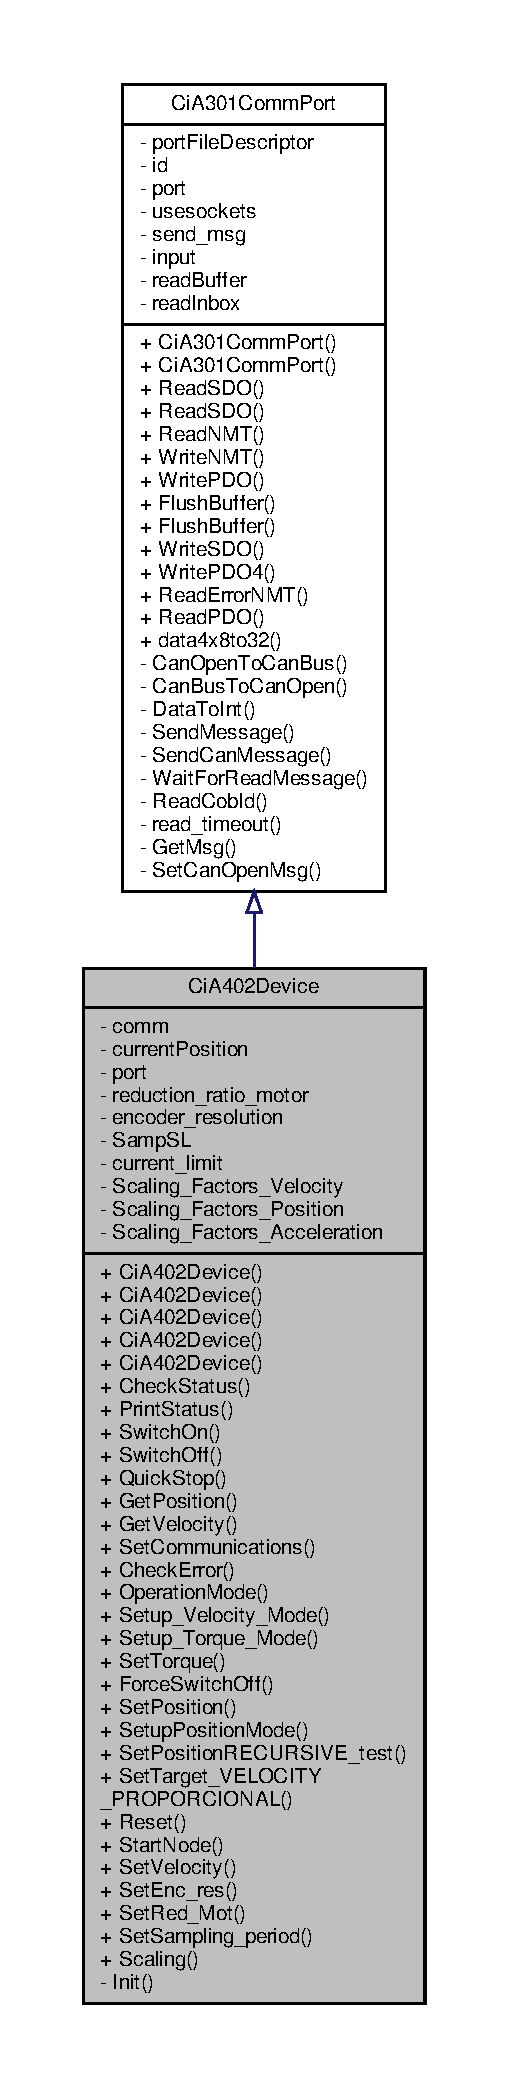
\includegraphics[height=550pt]{classCiA402Device__inherit__graph}
\end{center}
\end{figure}


Collaboration diagram for Ci\+A402\+Device\+:
\nopagebreak
\begin{figure}[H]
\begin{center}
\leavevmode
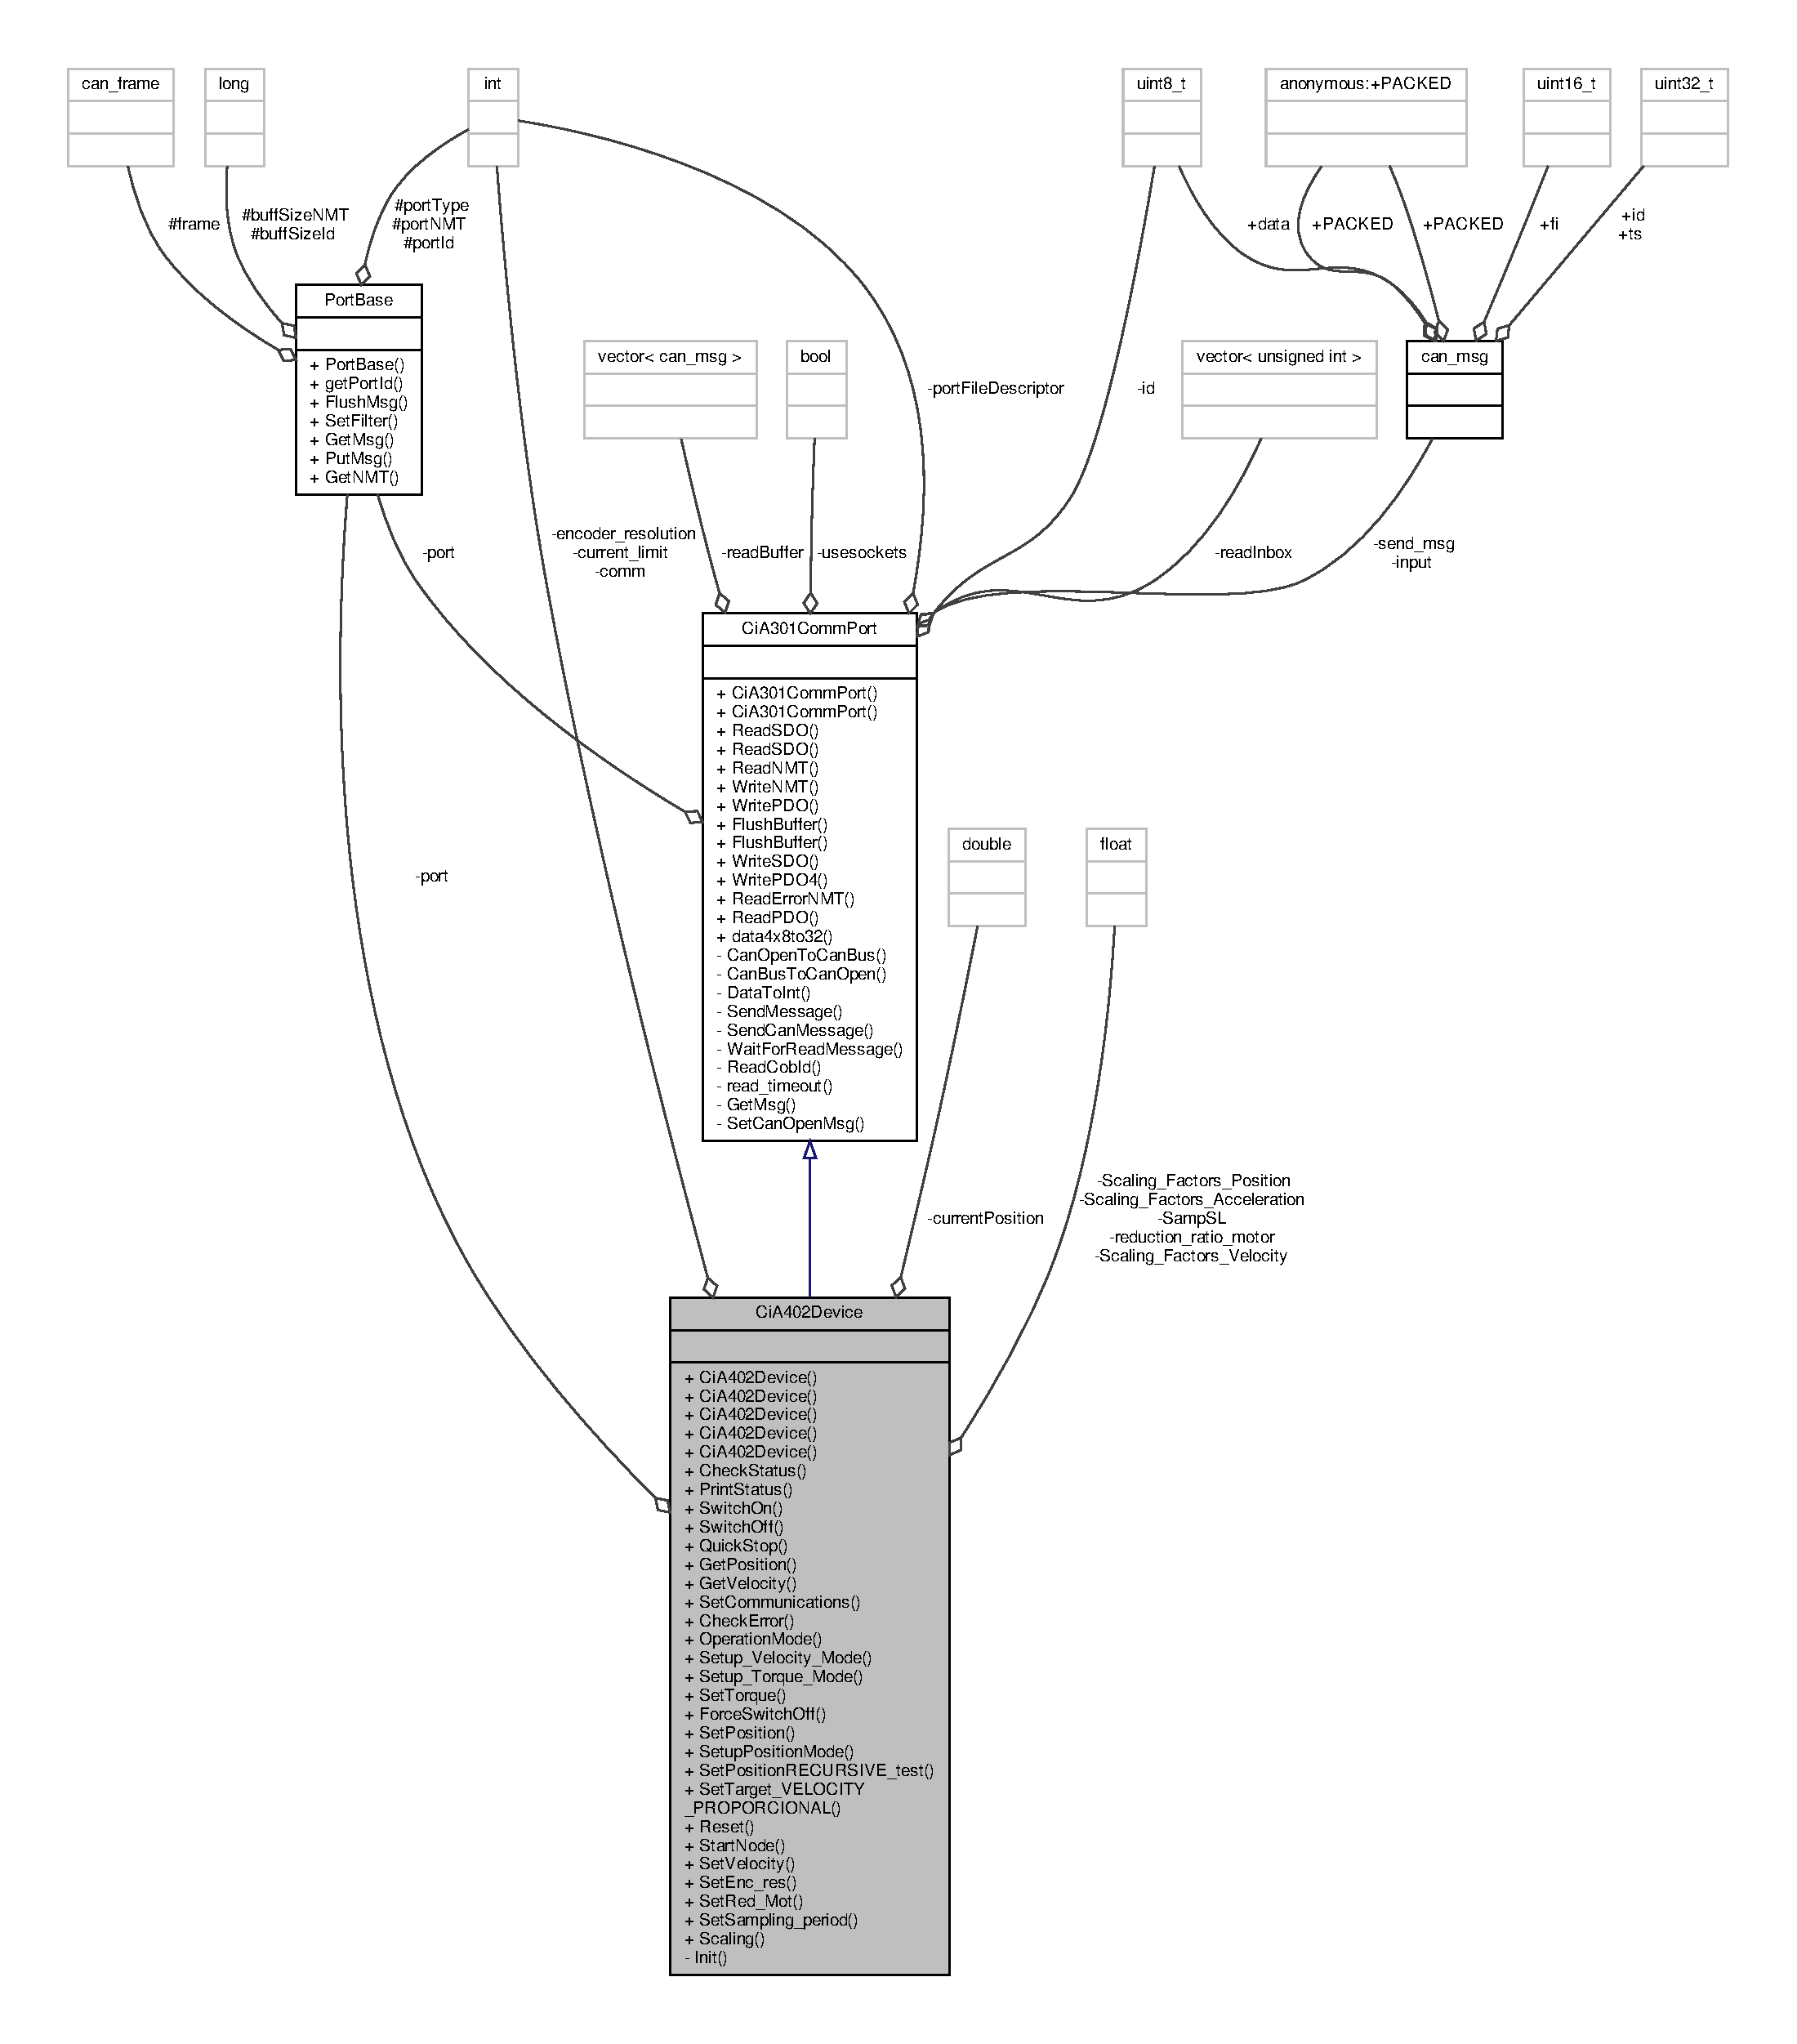
\includegraphics[width=350pt]{classCiA402Device__coll__graph}
\end{center}
\end{figure}
\subsection*{Public Member Functions}
\begin{DoxyCompactItemize}
\item 
\hyperlink{classCiA402Device_a894ef30b3c5a0ed291b086ad2156e4c1}{Ci\+A402\+Device} ()
\item 
\hyperlink{classCiA402Device_a77998e6d9ac4b75764612f3cab7426ef}{Ci\+A402\+Device} (uint8\+\_\+t new\+\_\+id)
\item 
\hyperlink{classCiA402Device_a084b18ac995775f5079c8b260ec4c6c8}{Ci\+A402\+Device} (uint8\+\_\+t new\+\_\+id, int fd\+Port)
\item 
\hyperlink{classCiA402Device_a017bcbc5d6e7a87b950b3cf2fcff1c41}{Ci\+A402\+Device} (uint8\+\_\+t new\+\_\+id, \hyperlink{classPortBase}{Port\+Base} $\ast$new\+\_\+port)
\item 
\hyperlink{classCiA402Device_a4c0e432fc2cc0189bd415904bdb0e31b}{Ci\+A402\+Device} (uint8\+\_\+t new\+\_\+id, \hyperlink{classPortBase}{Port\+Base} $\ast$new\+\_\+port, \hyperlink{classCiA402SetupData}{Ci\+A402\+Setup\+Data} $\ast$device\+Data)
\item 
uint16\+\_\+t \hyperlink{classCiA402Device_a5a034b00c87d2ec9ec98157b772465d9}{Check\+Status} ()
\begin{DoxyCompactList}\small\item\em Check\+Status\+: Returns the status word. \end{DoxyCompactList}\item 
void \hyperlink{classCiA402Device_a9d5d8df28085395a3ab711107a181ebc}{Print\+Status} ()
\begin{DoxyCompactList}\small\item\em Print\+Status\+: Print the status word. \end{DoxyCompactList}\item 
long \hyperlink{classCiA402Device_ab77bce0d7f42429f5f8f092aacb02754}{Switch\+On} ()
\begin{DoxyCompactList}\small\item\em Switch\+On\+: Turn on the device and wait for commands. \end{DoxyCompactList}\item 
long \hyperlink{classCiA402Device_a97acf47b3e3751c85fa70091d3bdfa6a}{Switch\+Off} ()
\begin{DoxyCompactList}\small\item\em Switch\+Off\+: Turn on the device. \end{DoxyCompactList}\item 
long \hyperlink{classCiA402Device_a8573afbf420c29aa86cd215d74f4e4e3}{Quick\+Stop} ()
\begin{DoxyCompactList}\small\item\em Quick\+Stop\+: Fast turn off of the device. \end{DoxyCompactList}\item 
double \hyperlink{classCiA402Device_ac8d9e36e6f457565cac7d26d91e4a712}{Get\+Position} ()
\begin{DoxyCompactList}\small\item\em Get\+Position\+: Get the position of the cia 402 device. \end{DoxyCompactList}\item 
double \hyperlink{classCiA402Device_a54b43f6429da4c6c0241653355e81d36}{Get\+Velocity} ()
\begin{DoxyCompactList}\small\item\em \hyperlink{classCiA402Device_a54b43f6429da4c6c0241653355e81d36}{Ci\+A402\+Device\+::\+Get\+Velocity} This function converts a variable of type uint32\+\_\+t which contains the equivalent velocity as function of the enconder lines/sample into the velocity of a motor with an encoder of X lines in radians per second. \end{DoxyCompactList}\item 
double \hyperlink{classCiA402Device_a436b9e3ba2d14367f0bba8d0fe977e23}{Get\+Filtered\+Velocity} (int samples)
\item 
double \hyperlink{classCiA402Device_aa19636eb332e6b3bc8265ecc3498f197}{Get\+Mean\+Velocity} ()
\item 
long \hyperlink{classCiA402Device_abf511a7d44b62ac93ae18fe21f8d51c9}{Set\+Communications} (int fd\+Port)
\item 
int \hyperlink{classCiA402Device_af1ed15805579e85e514e7ccf4ff21e10}{Check\+Error} ()
\item 
long \hyperlink{classCiA402Device_a49f298cf0d4d2d68007b3cb396e93a17}{Operation\+Mode} (const vector$<$ uint8\+\_\+t $>$ new\+\_\+mode)
\item 
long \hyperlink{classCiA402Device_acd659c05abd1534881a0cec2326d4ba8}{Setup\+\_\+\+Velocity\+\_\+\+Mode} (const uint32\+\_\+t target=0, const uint32\+\_\+t acceleration=1)
\item 
long \hyperlink{classCiA402Device_a20475438205c26cd4bcc689ed9c7fe95}{Setup\+\_\+\+Torque\+\_\+\+Mode} ()
\begin{DoxyCompactList}\small\item\em Ci\+A402\+Device\+::\+Degree\+Conv This function converts a variable of type uint32\+\_\+t which contains the position of a motor with an encoder of 4096 lines in decimal degrees into the equivalent position as function of the enconders lines. If the parameter has a value of 360 the function will return an uint32\+\_\+t variable with a value of 4096. \end{DoxyCompactList}\item 
long \hyperlink{classCiA402Device_a556c03984774974dd3a1231793916d9b}{Set\+Torque} (double target)
\item 
long \hyperlink{classCiA402Device_aff0503b4caa6d2a8e2e66df6b9e0f4e4}{Force\+Switch\+Off} ()
\item 
long \hyperlink{classCiA402Device_ac13cd5d90f8d39e1ef9734d035e67acb}{Set\+Position} (double target)
\begin{DoxyCompactList}\small\item\em \hyperlink{classCiA402Device_ac13cd5d90f8d39e1ef9734d035e67acb}{Ci\+A402\+Device\+::\+Set\+Position} This function performs the communication with the device to perform a position control in a motor and perform a motion towards a selected position. The motor remembers as position 0 the position in which it has been switched on, always returning to this position when its target is 0. \end{DoxyCompactList}\item 
long \hyperlink{classCiA402Device_a726ff3dfbfc8ae76c01d26277d0b764c}{Setup\+Position\+Mode} (const uint32\+\_\+t velocity=1, const uint32\+\_\+t acceleration=1)
\item 
long \hyperlink{classCiA402Device_ac1c55984abb91928d52b0a49651cc18e}{Set\+Position\+R\+E\+C\+U\+R\+S\+I\+V\+E\+\_\+test} (long target)
\item 
long \hyperlink{classCiA402Device_a1b88a18321d6dbee11258b48d49706ba}{Set\+Target\+\_\+\+V\+E\+L\+O\+C\+I\+T\+Y\+\_\+\+P\+R\+O\+P\+O\+R\+C\+I\+O\+N\+AL} (double target, float kp)
\item 
long \hyperlink{classCiA402Device_ac4a6e4987ebe075d0ac07ee5fd4d410c}{Reset} ()
\begin{DoxyCompactList}\small\item\em Reset This function resets the node corresponding to this object. \end{DoxyCompactList}\item 
long \hyperlink{classCiA402Device_a32b4628098364846fe291312025f6fda}{Start\+Node} ()
\item 
long \hyperlink{classCiA402Device_a498224b82a857197eb2d28beddc74729}{Set\+Velocity} (double target)
\begin{DoxyCompactList}\small\item\em \hyperlink{classCiA402Device_a498224b82a857197eb2d28beddc74729}{Ci\+A402\+Device\+::\+Set\+Velocity} This function converts the velocity of a motor with an encoder of X lines in radians per second into a variable of type uint32\+\_\+t which contains the equivalent velocity as function of the enconder lines/sample. \end{DoxyCompactList}\item 
long \hyperlink{classCiA402Device_a065607adbfdf2446887554b1a3192243}{Set\+Enc\+\_\+res} (int lines)
\begin{DoxyCompactList}\small\item\em Set the Nº lines for incremental encoder quadrature (lines X 4) \end{DoxyCompactList}\item 
long \hyperlink{classCiA402Device_ad5b57f2ddfc103644daf157dcd6ab34e}{Set\+Red\+\_\+\+Mot} (float reduction\+\_\+ratio)
\begin{DoxyCompactList}\small\item\em Set the transmission ratio between the motor displacement in SI units and load displacement. \end{DoxyCompactList}\item 
long \hyperlink{classCiA402Device_a9fc81b5fd6bec7cf73a1e60b92b7bfc0}{Set\+Sampling\+\_\+period} (float sampling\+\_\+period)
\begin{DoxyCompactList}\small\item\em Set the speed/position loop sampling period of the motor Control (sampling\+\_\+slow\+\_\+loop) \end{DoxyCompactList}\item 
long \hyperlink{classCiA402Device_ae9b30263a0592f0b254ae4f32cd9a765}{Scaling} (void)
\end{DoxyCompactItemize}
\subsection*{Private Member Functions}
\begin{DoxyCompactItemize}
\item 
long \hyperlink{classCiA402Device_abc4e196ca1654a71bc396d77580701f0}{Init} (\hyperlink{classCiA402SetupData}{Ci\+A402\+Setup\+Data} $\ast$device\+Data)
\end{DoxyCompactItemize}
\subsection*{Private Attributes}
\begin{DoxyCompactItemize}
\item 
int \hyperlink{classCiA402Device_a4e7a5a225fb27f5f02aeb0e6df38cd1f}{comm}
\item 
\hyperlink{classPortBase}{Port\+Base} $\ast$ \hyperlink{classCiA402Device_abc96eb117cc948d86e3bd4c07c7fe807}{port}
\item 
float \hyperlink{classCiA402Device_ad433f5fc62f2f7e78815807418ada3ba}{reduction\+\_\+ratio\+\_\+motor}
\item 
int \hyperlink{classCiA402Device_aab8a459615d73c60728344aaedc9f66c}{encoder\+\_\+resolution}
\item 
float \hyperlink{classCiA402Device_a5d0d4f4f4fcb7413e5de0270341fb209}{Samp\+SL}
\item 
int \hyperlink{classCiA402Device_a3dfe8b82f4049137b0992934a9239053}{current\+\_\+limit}
\item 
float \hyperlink{classCiA402Device_a57db6ccb730d3c26b7b33000d371b3bf}{Scaling\+\_\+\+Factors\+\_\+\+Velocity}
\item 
float \hyperlink{classCiA402Device_af6df63ddd2ddc1953f847855436ef129}{Scaling\+\_\+\+Factors\+\_\+\+Position}
\item 
float \hyperlink{classCiA402Device_a59de671e30be6f3f8f4c6ede7595d16c}{Scaling\+\_\+\+Factors\+\_\+\+Acceleration}
\item 
double \hyperlink{classCiA402Device_adb251ae496aeca707dcc51b43c64d0b8}{current\+Position}
\item 
double \hyperlink{classCiA402Device_a18ab540b52f7de30257f92340583a750}{last\+Position}
\item 
double \hyperlink{classCiA402Device_af926910c5a7e80c6ec198e1bd110b8d1}{mean\+Velocity}
\item 
chrono\+::system\+\_\+clock\+::time\+\_\+point \hyperlink{classCiA402Device_a2bd9cbd37d46453520e6fba51e720215}{actual\+Time\+Value}
\item 
chrono\+::system\+\_\+clock\+::time\+\_\+point \hyperlink{classCiA402Device_a3877e4a9b429edbac68503a828dd349d}{last\+Time\+Value}
\item 
chrono\+::system\+\_\+clock\+::time\+\_\+point \hyperlink{classCiA402Device_afb0d98f7068e7373f6d7b54d149f0680}{encoder\+Change\+Time}
\item 
double \hyperlink{classCiA402Device_a332cd74ce718607e9359b3db0f9ac402}{encoder\+Span}
\item 
chrono\+::nanoseconds \hyperlink{classCiA402Device_af3e9acfa1412aad23657a97464626f1d}{dts\+Wait}
\item 
chrono\+::nanoseconds \hyperlink{classCiA402Device_ad44fd620387924741772ab8e02d8b95a}{t\+Waited}
\end{DoxyCompactItemize}


\subsection{Constructor \& Destructor Documentation}
\index{Ci\+A402\+Device@{Ci\+A402\+Device}!Ci\+A402\+Device@{Ci\+A402\+Device}}
\index{Ci\+A402\+Device@{Ci\+A402\+Device}!Ci\+A402\+Device@{Ci\+A402\+Device}}
\subsubsection[{\texorpdfstring{Ci\+A402\+Device()}{CiA402Device()}}]{\setlength{\rightskip}{0pt plus 5cm}Ci\+A402\+Device\+::\+Ci\+A402\+Device (
\begin{DoxyParamCaption}
{}
\end{DoxyParamCaption}
)}\hypertarget{classCiA402Device_a894ef30b3c5a0ed291b086ad2156e4c1}{}\label{classCiA402Device_a894ef30b3c5a0ed291b086ad2156e4c1}
\index{Ci\+A402\+Device@{Ci\+A402\+Device}!Ci\+A402\+Device@{Ci\+A402\+Device}}
\index{Ci\+A402\+Device@{Ci\+A402\+Device}!Ci\+A402\+Device@{Ci\+A402\+Device}}
\subsubsection[{\texorpdfstring{Ci\+A402\+Device(uint8\+\_\+t new\+\_\+id)}{CiA402Device(uint8_t new_id)}}]{\setlength{\rightskip}{0pt plus 5cm}Ci\+A402\+Device\+::\+Ci\+A402\+Device (
\begin{DoxyParamCaption}
\item[{uint8\+\_\+t}]{new\+\_\+id}
\end{DoxyParamCaption}
)}\hypertarget{classCiA402Device_a77998e6d9ac4b75764612f3cab7426ef}{}\label{classCiA402Device_a77998e6d9ac4b75764612f3cab7426ef}
\index{Ci\+A402\+Device@{Ci\+A402\+Device}!Ci\+A402\+Device@{Ci\+A402\+Device}}
\index{Ci\+A402\+Device@{Ci\+A402\+Device}!Ci\+A402\+Device@{Ci\+A402\+Device}}
\subsubsection[{\texorpdfstring{Ci\+A402\+Device(uint8\+\_\+t new\+\_\+id, int fd\+Port)}{CiA402Device(uint8_t new_id, int fdPort)}}]{\setlength{\rightskip}{0pt plus 5cm}Ci\+A402\+Device\+::\+Ci\+A402\+Device (
\begin{DoxyParamCaption}
\item[{uint8\+\_\+t}]{new\+\_\+id, }
\item[{int}]{fd\+Port}
\end{DoxyParamCaption}
)}\hypertarget{classCiA402Device_a084b18ac995775f5079c8b260ec4c6c8}{}\label{classCiA402Device_a084b18ac995775f5079c8b260ec4c6c8}
\index{Ci\+A402\+Device@{Ci\+A402\+Device}!Ci\+A402\+Device@{Ci\+A402\+Device}}
\index{Ci\+A402\+Device@{Ci\+A402\+Device}!Ci\+A402\+Device@{Ci\+A402\+Device}}
\subsubsection[{\texorpdfstring{Ci\+A402\+Device(uint8\+\_\+t new\+\_\+id, Port\+Base $\ast$new\+\_\+port)}{CiA402Device(uint8_t new_id, PortBase *new_port)}}]{\setlength{\rightskip}{0pt plus 5cm}Ci\+A402\+Device\+::\+Ci\+A402\+Device (
\begin{DoxyParamCaption}
\item[{uint8\+\_\+t}]{new\+\_\+id, }
\item[{{\bf Port\+Base} $\ast$}]{new\+\_\+port}
\end{DoxyParamCaption}
)}\hypertarget{classCiA402Device_a017bcbc5d6e7a87b950b3cf2fcff1c41}{}\label{classCiA402Device_a017bcbc5d6e7a87b950b3cf2fcff1c41}
\index{Ci\+A402\+Device@{Ci\+A402\+Device}!Ci\+A402\+Device@{Ci\+A402\+Device}}
\index{Ci\+A402\+Device@{Ci\+A402\+Device}!Ci\+A402\+Device@{Ci\+A402\+Device}}
\subsubsection[{\texorpdfstring{Ci\+A402\+Device(uint8\+\_\+t new\+\_\+id, Port\+Base $\ast$new\+\_\+port, Ci\+A402\+Setup\+Data $\ast$device\+Data)}{CiA402Device(uint8_t new_id, PortBase *new_port, CiA402SetupData *deviceData)}}]{\setlength{\rightskip}{0pt plus 5cm}Ci\+A402\+Device\+::\+Ci\+A402\+Device (
\begin{DoxyParamCaption}
\item[{uint8\+\_\+t}]{new\+\_\+id, }
\item[{{\bf Port\+Base} $\ast$}]{new\+\_\+port, }
\item[{{\bf Ci\+A402\+Setup\+Data} $\ast$}]{device\+Data}
\end{DoxyParamCaption}
)}\hypertarget{classCiA402Device_a4c0e432fc2cc0189bd415904bdb0e31b}{}\label{classCiA402Device_a4c0e432fc2cc0189bd415904bdb0e31b}


\subsection{Member Function Documentation}
\index{Ci\+A402\+Device@{Ci\+A402\+Device}!Check\+Error@{Check\+Error}}
\index{Check\+Error@{Check\+Error}!Ci\+A402\+Device@{Ci\+A402\+Device}}
\subsubsection[{\texorpdfstring{Check\+Error()}{CheckError()}}]{\setlength{\rightskip}{0pt plus 5cm}int Ci\+A402\+Device\+::\+Check\+Error (
\begin{DoxyParamCaption}
{}
\end{DoxyParamCaption}
)}\hypertarget{classCiA402Device_af1ed15805579e85e514e7ccf4ff21e10}{}\label{classCiA402Device_af1ed15805579e85e514e7ccf4ff21e10}
\index{Ci\+A402\+Device@{Ci\+A402\+Device}!Check\+Status@{Check\+Status}}
\index{Check\+Status@{Check\+Status}!Ci\+A402\+Device@{Ci\+A402\+Device}}
\subsubsection[{\texorpdfstring{Check\+Status()}{CheckStatus()}}]{\setlength{\rightskip}{0pt plus 5cm}uint16\+\_\+t Ci\+A402\+Device\+::\+Check\+Status (
\begin{DoxyParamCaption}
{}
\end{DoxyParamCaption}
)}\hypertarget{classCiA402Device_a5a034b00c87d2ec9ec98157b772465d9}{}\label{classCiA402Device_a5a034b00c87d2ec9ec98157b772465d9}


Check\+Status\+: Returns the status word. 

\begin{DoxyReturn}{Returns}
\+: status 
\end{DoxyReturn}
\index{Ci\+A402\+Device@{Ci\+A402\+Device}!Force\+Switch\+Off@{Force\+Switch\+Off}}
\index{Force\+Switch\+Off@{Force\+Switch\+Off}!Ci\+A402\+Device@{Ci\+A402\+Device}}
\subsubsection[{\texorpdfstring{Force\+Switch\+Off()}{ForceSwitchOff()}}]{\setlength{\rightskip}{0pt plus 5cm}long Ci\+A402\+Device\+::\+Force\+Switch\+Off (
\begin{DoxyParamCaption}
{}
\end{DoxyParamCaption}
)}\hypertarget{classCiA402Device_aff0503b4caa6d2a8e2e66df6b9e0f4e4}{}\label{classCiA402Device_aff0503b4caa6d2a8e2e66df6b9e0f4e4}
\index{Ci\+A402\+Device@{Ci\+A402\+Device}!Get\+Filtered\+Velocity@{Get\+Filtered\+Velocity}}
\index{Get\+Filtered\+Velocity@{Get\+Filtered\+Velocity}!Ci\+A402\+Device@{Ci\+A402\+Device}}
\subsubsection[{\texorpdfstring{Get\+Filtered\+Velocity(int samples)}{GetFilteredVelocity(int samples)}}]{\setlength{\rightskip}{0pt plus 5cm}double Ci\+A402\+Device\+::\+Get\+Filtered\+Velocity (
\begin{DoxyParamCaption}
\item[{int}]{samples}
\end{DoxyParamCaption}
)}\hypertarget{classCiA402Device_a436b9e3ba2d14367f0bba8d0fe977e23}{}\label{classCiA402Device_a436b9e3ba2d14367f0bba8d0fe977e23}
\index{Ci\+A402\+Device@{Ci\+A402\+Device}!Get\+Mean\+Velocity@{Get\+Mean\+Velocity}}
\index{Get\+Mean\+Velocity@{Get\+Mean\+Velocity}!Ci\+A402\+Device@{Ci\+A402\+Device}}
\subsubsection[{\texorpdfstring{Get\+Mean\+Velocity()}{GetMeanVelocity()}}]{\setlength{\rightskip}{0pt plus 5cm}double Ci\+A402\+Device\+::\+Get\+Mean\+Velocity (
\begin{DoxyParamCaption}
{}
\end{DoxyParamCaption}
)}\hypertarget{classCiA402Device_aa19636eb332e6b3bc8265ecc3498f197}{}\label{classCiA402Device_aa19636eb332e6b3bc8265ecc3498f197}
\index{Ci\+A402\+Device@{Ci\+A402\+Device}!Get\+Position@{Get\+Position}}
\index{Get\+Position@{Get\+Position}!Ci\+A402\+Device@{Ci\+A402\+Device}}
\subsubsection[{\texorpdfstring{Get\+Position()}{GetPosition()}}]{\setlength{\rightskip}{0pt plus 5cm}double Ci\+A402\+Device\+::\+Get\+Position (
\begin{DoxyParamCaption}
{}
\end{DoxyParamCaption}
)}\hypertarget{classCiA402Device_ac8d9e36e6f457565cac7d26d91e4a712}{}\label{classCiA402Device_ac8d9e36e6f457565cac7d26d91e4a712}


Get\+Position\+: Get the position of the cia 402 device. 

\begin{DoxyReturn}{Returns}
\+: Position (angle in \mbox{[}rad\mbox{]}) 
\end{DoxyReturn}
\index{Ci\+A402\+Device@{Ci\+A402\+Device}!Get\+Velocity@{Get\+Velocity}}
\index{Get\+Velocity@{Get\+Velocity}!Ci\+A402\+Device@{Ci\+A402\+Device}}
\subsubsection[{\texorpdfstring{Get\+Velocity()}{GetVelocity()}}]{\setlength{\rightskip}{0pt plus 5cm}double Ci\+A402\+Device\+::\+Get\+Velocity (
\begin{DoxyParamCaption}
{}
\end{DoxyParamCaption}
)}\hypertarget{classCiA402Device_a54b43f6429da4c6c0241653355e81d36}{}\label{classCiA402Device_a54b43f6429da4c6c0241653355e81d36}


\hyperlink{classCiA402Device_a54b43f6429da4c6c0241653355e81d36}{Ci\+A402\+Device\+::\+Get\+Velocity} This function converts a variable of type uint32\+\_\+t which contains the equivalent velocity as function of the enconder lines/sample into the velocity of a motor with an encoder of X lines in radians per second. 

\begin{DoxyReturn}{Returns}
This function returns a variable of type double with value the actual velocity in rad/s 
\end{DoxyReturn}
\index{Ci\+A402\+Device@{Ci\+A402\+Device}!Init@{Init}}
\index{Init@{Init}!Ci\+A402\+Device@{Ci\+A402\+Device}}
\subsubsection[{\texorpdfstring{Init(\+Ci\+A402\+Setup\+Data $\ast$device\+Data)}{Init(CiA402SetupData *deviceData)}}]{\setlength{\rightskip}{0pt plus 5cm}long Ci\+A402\+Device\+::\+Init (
\begin{DoxyParamCaption}
\item[{{\bf Ci\+A402\+Setup\+Data} $\ast$}]{device\+Data}
\end{DoxyParamCaption}
)\hspace{0.3cm}{\ttfamily [private]}}\hypertarget{classCiA402Device_abc4e196ca1654a71bc396d77580701f0}{}\label{classCiA402Device_abc4e196ca1654a71bc396d77580701f0}
\index{Ci\+A402\+Device@{Ci\+A402\+Device}!Operation\+Mode@{Operation\+Mode}}
\index{Operation\+Mode@{Operation\+Mode}!Ci\+A402\+Device@{Ci\+A402\+Device}}
\subsubsection[{\texorpdfstring{Operation\+Mode(const vector$<$ uint8\+\_\+t $>$ new\+\_\+mode)}{OperationMode(const vector< uint8_t > new_mode)}}]{\setlength{\rightskip}{0pt plus 5cm}long Ci\+A402\+Device\+::\+Operation\+Mode (
\begin{DoxyParamCaption}
\item[{const vector$<$ uint8\+\_\+t $>$}]{new\+\_\+mode}
\end{DoxyParamCaption}
)}\hypertarget{classCiA402Device_a49f298cf0d4d2d68007b3cb396e93a17}{}\label{classCiA402Device_a49f298cf0d4d2d68007b3cb396e93a17}
\index{Ci\+A402\+Device@{Ci\+A402\+Device}!Print\+Status@{Print\+Status}}
\index{Print\+Status@{Print\+Status}!Ci\+A402\+Device@{Ci\+A402\+Device}}
\subsubsection[{\texorpdfstring{Print\+Status()}{PrintStatus()}}]{\setlength{\rightskip}{0pt plus 5cm}void Ci\+A402\+Device\+::\+Print\+Status (
\begin{DoxyParamCaption}
{}
\end{DoxyParamCaption}
)}\hypertarget{classCiA402Device_a9d5d8df28085395a3ab711107a181ebc}{}\label{classCiA402Device_a9d5d8df28085395a3ab711107a181ebc}


Print\+Status\+: Print the status word. 

\begin{DoxyReturn}{Returns}
\+: 0 if correct, negative on errors. 
\end{DoxyReturn}
\index{Ci\+A402\+Device@{Ci\+A402\+Device}!Quick\+Stop@{Quick\+Stop}}
\index{Quick\+Stop@{Quick\+Stop}!Ci\+A402\+Device@{Ci\+A402\+Device}}
\subsubsection[{\texorpdfstring{Quick\+Stop()}{QuickStop()}}]{\setlength{\rightskip}{0pt plus 5cm}long Ci\+A402\+Device\+::\+Quick\+Stop (
\begin{DoxyParamCaption}
{}
\end{DoxyParamCaption}
)}\hypertarget{classCiA402Device_a8573afbf420c29aa86cd215d74f4e4e3}{}\label{classCiA402Device_a8573afbf420c29aa86cd215d74f4e4e3}


Quick\+Stop\+: Fast turn off of the device. 

\begin{DoxyReturn}{Returns}
\+: 0 if correct, negative on errors. 
\end{DoxyReturn}
\index{Ci\+A402\+Device@{Ci\+A402\+Device}!Reset@{Reset}}
\index{Reset@{Reset}!Ci\+A402\+Device@{Ci\+A402\+Device}}
\subsubsection[{\texorpdfstring{Reset()}{Reset()}}]{\setlength{\rightskip}{0pt plus 5cm}long Ci\+A402\+Device\+::\+Reset (
\begin{DoxyParamCaption}
{}
\end{DoxyParamCaption}
)}\hypertarget{classCiA402Device_ac4a6e4987ebe075d0ac07ee5fd4d410c}{}\label{classCiA402Device_ac4a6e4987ebe075d0ac07ee5fd4d410c}


Reset This function resets the node corresponding to this object. 

\begin{DoxyReturn}{Returns}
a long of value 0 if there are no errors. 
\end{DoxyReturn}
\index{Ci\+A402\+Device@{Ci\+A402\+Device}!Scaling@{Scaling}}
\index{Scaling@{Scaling}!Ci\+A402\+Device@{Ci\+A402\+Device}}
\subsubsection[{\texorpdfstring{Scaling(void)}{Scaling(void)}}]{\setlength{\rightskip}{0pt plus 5cm}long Ci\+A402\+Device\+::\+Scaling (
\begin{DoxyParamCaption}
\item[{void}]{}
\end{DoxyParamCaption}
)}\hypertarget{classCiA402Device_ae9b30263a0592f0b254ae4f32cd9a765}{}\label{classCiA402Device_ae9b30263a0592f0b254ae4f32cd9a765}
\index{Ci\+A402\+Device@{Ci\+A402\+Device}!Set\+Communications@{Set\+Communications}}
\index{Set\+Communications@{Set\+Communications}!Ci\+A402\+Device@{Ci\+A402\+Device}}
\subsubsection[{\texorpdfstring{Set\+Communications(int fd\+Port)}{SetCommunications(int fdPort)}}]{\setlength{\rightskip}{0pt plus 5cm}long Ci\+A402\+Device\+::\+Set\+Communications (
\begin{DoxyParamCaption}
\item[{int}]{fd\+Port}
\end{DoxyParamCaption}
)}\hypertarget{classCiA402Device_abf511a7d44b62ac93ae18fe21f8d51c9}{}\label{classCiA402Device_abf511a7d44b62ac93ae18fe21f8d51c9}
\index{Ci\+A402\+Device@{Ci\+A402\+Device}!Set\+Enc\+\_\+res@{Set\+Enc\+\_\+res}}
\index{Set\+Enc\+\_\+res@{Set\+Enc\+\_\+res}!Ci\+A402\+Device@{Ci\+A402\+Device}}
\subsubsection[{\texorpdfstring{Set\+Enc\+\_\+res(int lines)}{SetEnc_res(int lines)}}]{\setlength{\rightskip}{0pt plus 5cm}long Ci\+A402\+Device\+::\+Set\+Enc\+\_\+res (
\begin{DoxyParamCaption}
\item[{int}]{lines}
\end{DoxyParamCaption}
)}\hypertarget{classCiA402Device_a065607adbfdf2446887554b1a3192243}{}\label{classCiA402Device_a065607adbfdf2446887554b1a3192243}


Set the Nº lines for incremental encoder quadrature (lines X 4) 

\index{Ci\+A402\+Device@{Ci\+A402\+Device}!Set\+Position@{Set\+Position}}
\index{Set\+Position@{Set\+Position}!Ci\+A402\+Device@{Ci\+A402\+Device}}
\subsubsection[{\texorpdfstring{Set\+Position(double target)}{SetPosition(double target)}}]{\setlength{\rightskip}{0pt plus 5cm}long Ci\+A402\+Device\+::\+Set\+Position (
\begin{DoxyParamCaption}
\item[{double}]{target}
\end{DoxyParamCaption}
)}\hypertarget{classCiA402Device_ac13cd5d90f8d39e1ef9734d035e67acb}{}\label{classCiA402Device_ac13cd5d90f8d39e1ef9734d035e67acb}


\hyperlink{classCiA402Device_ac13cd5d90f8d39e1ef9734d035e67acb}{Ci\+A402\+Device\+::\+Set\+Position} This function performs the communication with the device to perform a position control in a motor and perform a motion towards a selected position. The motor remembers as position 0 the position in which it has been switched on, always returning to this position when its target is 0. 


\begin{DoxyParams}{Parameters}
{\em target} & of type uint32\+\_\+t is the desired position by means of the enconder lines. If this value is bigger than the number of lines of the enconder used, the motor\textquotesingle{}s axis will perform more than one turn. \\
\hline
\end{DoxyParams}
\begin{DoxyReturn}{Returns}
This function returns a variable of type long with value 0. 
\end{DoxyReturn}
\index{Ci\+A402\+Device@{Ci\+A402\+Device}!Set\+Position\+R\+E\+C\+U\+R\+S\+I\+V\+E\+\_\+test@{Set\+Position\+R\+E\+C\+U\+R\+S\+I\+V\+E\+\_\+test}}
\index{Set\+Position\+R\+E\+C\+U\+R\+S\+I\+V\+E\+\_\+test@{Set\+Position\+R\+E\+C\+U\+R\+S\+I\+V\+E\+\_\+test}!Ci\+A402\+Device@{Ci\+A402\+Device}}
\subsubsection[{\texorpdfstring{Set\+Position\+R\+E\+C\+U\+R\+S\+I\+V\+E\+\_\+test(long target)}{SetPositionRECURSIVE_test(long target)}}]{\setlength{\rightskip}{0pt plus 5cm}long Ci\+A402\+Device\+::\+Set\+Position\+R\+E\+C\+U\+R\+S\+I\+V\+E\+\_\+test (
\begin{DoxyParamCaption}
\item[{long}]{target}
\end{DoxyParamCaption}
)}\hypertarget{classCiA402Device_ac1c55984abb91928d52b0a49651cc18e}{}\label{classCiA402Device_ac1c55984abb91928d52b0a49651cc18e}
\index{Ci\+A402\+Device@{Ci\+A402\+Device}!Set\+Red\+\_\+\+Mot@{Set\+Red\+\_\+\+Mot}}
\index{Set\+Red\+\_\+\+Mot@{Set\+Red\+\_\+\+Mot}!Ci\+A402\+Device@{Ci\+A402\+Device}}
\subsubsection[{\texorpdfstring{Set\+Red\+\_\+\+Mot(float reduction\+\_\+ratio)}{SetRed_Mot(float reduction_ratio)}}]{\setlength{\rightskip}{0pt plus 5cm}long Ci\+A402\+Device\+::\+Set\+Red\+\_\+\+Mot (
\begin{DoxyParamCaption}
\item[{float}]{reduction\+\_\+ratio}
\end{DoxyParamCaption}
)}\hypertarget{classCiA402Device_ad5b57f2ddfc103644daf157dcd6ab34e}{}\label{classCiA402Device_ad5b57f2ddfc103644daf157dcd6ab34e}


Set the transmission ratio between the motor displacement in SI units and load displacement. 

\index{Ci\+A402\+Device@{Ci\+A402\+Device}!Set\+Sampling\+\_\+period@{Set\+Sampling\+\_\+period}}
\index{Set\+Sampling\+\_\+period@{Set\+Sampling\+\_\+period}!Ci\+A402\+Device@{Ci\+A402\+Device}}
\subsubsection[{\texorpdfstring{Set\+Sampling\+\_\+period(float sampling\+\_\+period)}{SetSampling_period(float sampling_period)}}]{\setlength{\rightskip}{0pt plus 5cm}long Ci\+A402\+Device\+::\+Set\+Sampling\+\_\+period (
\begin{DoxyParamCaption}
\item[{float}]{sampling\+\_\+period}
\end{DoxyParamCaption}
)}\hypertarget{classCiA402Device_a9fc81b5fd6bec7cf73a1e60b92b7bfc0}{}\label{classCiA402Device_a9fc81b5fd6bec7cf73a1e60b92b7bfc0}


Set the speed/position loop sampling period of the motor Control (sampling\+\_\+slow\+\_\+loop) 

\index{Ci\+A402\+Device@{Ci\+A402\+Device}!Set\+Target\+\_\+\+V\+E\+L\+O\+C\+I\+T\+Y\+\_\+\+P\+R\+O\+P\+O\+R\+C\+I\+O\+N\+AL@{Set\+Target\+\_\+\+V\+E\+L\+O\+C\+I\+T\+Y\+\_\+\+P\+R\+O\+P\+O\+R\+C\+I\+O\+N\+AL}}
\index{Set\+Target\+\_\+\+V\+E\+L\+O\+C\+I\+T\+Y\+\_\+\+P\+R\+O\+P\+O\+R\+C\+I\+O\+N\+AL@{Set\+Target\+\_\+\+V\+E\+L\+O\+C\+I\+T\+Y\+\_\+\+P\+R\+O\+P\+O\+R\+C\+I\+O\+N\+AL}!Ci\+A402\+Device@{Ci\+A402\+Device}}
\subsubsection[{\texorpdfstring{Set\+Target\+\_\+\+V\+E\+L\+O\+C\+I\+T\+Y\+\_\+\+P\+R\+O\+P\+O\+R\+C\+I\+O\+N\+A\+L(double target, float kp)}{SetTarget_VELOCITY_PROPORCIONAL(double target, float kp)}}]{\setlength{\rightskip}{0pt plus 5cm}long Ci\+A402\+Device\+::\+Set\+Target\+\_\+\+V\+E\+L\+O\+C\+I\+T\+Y\+\_\+\+P\+R\+O\+P\+O\+R\+C\+I\+O\+N\+AL (
\begin{DoxyParamCaption}
\item[{double}]{target, }
\item[{float}]{kp}
\end{DoxyParamCaption}
)}\hypertarget{classCiA402Device_a1b88a18321d6dbee11258b48d49706ba}{}\label{classCiA402Device_a1b88a18321d6dbee11258b48d49706ba}
\index{Ci\+A402\+Device@{Ci\+A402\+Device}!Set\+Torque@{Set\+Torque}}
\index{Set\+Torque@{Set\+Torque}!Ci\+A402\+Device@{Ci\+A402\+Device}}
\subsubsection[{\texorpdfstring{Set\+Torque(double target)}{SetTorque(double target)}}]{\setlength{\rightskip}{0pt plus 5cm}long Ci\+A402\+Device\+::\+Set\+Torque (
\begin{DoxyParamCaption}
\item[{double}]{target}
\end{DoxyParamCaption}
)}\hypertarget{classCiA402Device_a556c03984774974dd3a1231793916d9b}{}\label{classCiA402Device_a556c03984774974dd3a1231793916d9b}
\index{Ci\+A402\+Device@{Ci\+A402\+Device}!Setup\+\_\+\+Torque\+\_\+\+Mode@{Setup\+\_\+\+Torque\+\_\+\+Mode}}
\index{Setup\+\_\+\+Torque\+\_\+\+Mode@{Setup\+\_\+\+Torque\+\_\+\+Mode}!Ci\+A402\+Device@{Ci\+A402\+Device}}
\subsubsection[{\texorpdfstring{Setup\+\_\+\+Torque\+\_\+\+Mode()}{Setup_Torque_Mode()}}]{\setlength{\rightskip}{0pt plus 5cm}long Ci\+A402\+Device\+::\+Setup\+\_\+\+Torque\+\_\+\+Mode (
\begin{DoxyParamCaption}
{}
\end{DoxyParamCaption}
)}\hypertarget{classCiA402Device_a20475438205c26cd4bcc689ed9c7fe95}{}\label{classCiA402Device_a20475438205c26cd4bcc689ed9c7fe95}


Ci\+A402\+Device\+::\+Degree\+Conv This function converts a variable of type uint32\+\_\+t which contains the position of a motor with an encoder of 4096 lines in decimal degrees into the equivalent position as function of the enconders lines. If the parameter has a value of 360 the function will return an uint32\+\_\+t variable with a value of 4096. 


\begin{DoxyParams}{Parameters}
{\em Degree\+Target} & A uint32\+\_\+t variable with the desired position in decimal degrees \\
\hline
\end{DoxyParams}
\begin{DoxyReturn}{Returns}
target\+Pos A uint32\+\_\+t variable with the equivalent position as a function of the encoder lines. 
\end{DoxyReturn}
\index{Ci\+A402\+Device@{Ci\+A402\+Device}!Setup\+\_\+\+Velocity\+\_\+\+Mode@{Setup\+\_\+\+Velocity\+\_\+\+Mode}}
\index{Setup\+\_\+\+Velocity\+\_\+\+Mode@{Setup\+\_\+\+Velocity\+\_\+\+Mode}!Ci\+A402\+Device@{Ci\+A402\+Device}}
\subsubsection[{\texorpdfstring{Setup\+\_\+\+Velocity\+\_\+\+Mode(const uint32\+\_\+t target=0, const uint32\+\_\+t acceleration=1)}{Setup_Velocity_Mode(const uint32_t target=0, const uint32_t acceleration=1)}}]{\setlength{\rightskip}{0pt plus 5cm}long Ci\+A402\+Device\+::\+Setup\+\_\+\+Velocity\+\_\+\+Mode (
\begin{DoxyParamCaption}
\item[{const uint32\+\_\+t}]{target = {\ttfamily 0}, }
\item[{const uint32\+\_\+t}]{acceleration = {\ttfamily 1}}
\end{DoxyParamCaption}
)}\hypertarget{classCiA402Device_acd659c05abd1534881a0cec2326d4ba8}{}\label{classCiA402Device_acd659c05abd1534881a0cec2326d4ba8}
\index{Ci\+A402\+Device@{Ci\+A402\+Device}!Setup\+Position\+Mode@{Setup\+Position\+Mode}}
\index{Setup\+Position\+Mode@{Setup\+Position\+Mode}!Ci\+A402\+Device@{Ci\+A402\+Device}}
\subsubsection[{\texorpdfstring{Setup\+Position\+Mode(const uint32\+\_\+t velocity=1, const uint32\+\_\+t acceleration=1)}{SetupPositionMode(const uint32_t velocity=1, const uint32_t acceleration=1)}}]{\setlength{\rightskip}{0pt plus 5cm}long Ci\+A402\+Device\+::\+Setup\+Position\+Mode (
\begin{DoxyParamCaption}
\item[{const uint32\+\_\+t}]{velocity = {\ttfamily 1}, }
\item[{const uint32\+\_\+t}]{acceleration = {\ttfamily 1}}
\end{DoxyParamCaption}
)}\hypertarget{classCiA402Device_a726ff3dfbfc8ae76c01d26277d0b764c}{}\label{classCiA402Device_a726ff3dfbfc8ae76c01d26277d0b764c}
\index{Ci\+A402\+Device@{Ci\+A402\+Device}!Set\+Velocity@{Set\+Velocity}}
\index{Set\+Velocity@{Set\+Velocity}!Ci\+A402\+Device@{Ci\+A402\+Device}}
\subsubsection[{\texorpdfstring{Set\+Velocity(double target)}{SetVelocity(double target)}}]{\setlength{\rightskip}{0pt plus 5cm}long Ci\+A402\+Device\+::\+Set\+Velocity (
\begin{DoxyParamCaption}
\item[{double}]{target}
\end{DoxyParamCaption}
)}\hypertarget{classCiA402Device_a498224b82a857197eb2d28beddc74729}{}\label{classCiA402Device_a498224b82a857197eb2d28beddc74729}


\hyperlink{classCiA402Device_a498224b82a857197eb2d28beddc74729}{Ci\+A402\+Device\+::\+Set\+Velocity} This function converts the velocity of a motor with an encoder of X lines in radians per second into a variable of type uint32\+\_\+t which contains the equivalent velocity as function of the enconder lines/sample. 


\begin{DoxyParams}{Parameters}
{\em target} & A uint32\+\_\+t variable with the desired velocity in rad/s \\
\hline
\end{DoxyParams}
\begin{DoxyReturn}{Returns}
This function re1turns a variable of type long with value 0. 
\end{DoxyReturn}
\index{Ci\+A402\+Device@{Ci\+A402\+Device}!Start\+Node@{Start\+Node}}
\index{Start\+Node@{Start\+Node}!Ci\+A402\+Device@{Ci\+A402\+Device}}
\subsubsection[{\texorpdfstring{Start\+Node()}{StartNode()}}]{\setlength{\rightskip}{0pt plus 5cm}long Ci\+A402\+Device\+::\+Start\+Node (
\begin{DoxyParamCaption}
{}
\end{DoxyParamCaption}
)}\hypertarget{classCiA402Device_a32b4628098364846fe291312025f6fda}{}\label{classCiA402Device_a32b4628098364846fe291312025f6fda}
\index{Ci\+A402\+Device@{Ci\+A402\+Device}!Switch\+Off@{Switch\+Off}}
\index{Switch\+Off@{Switch\+Off}!Ci\+A402\+Device@{Ci\+A402\+Device}}
\subsubsection[{\texorpdfstring{Switch\+Off()}{SwitchOff()}}]{\setlength{\rightskip}{0pt plus 5cm}long Ci\+A402\+Device\+::\+Switch\+Off (
\begin{DoxyParamCaption}
{}
\end{DoxyParamCaption}
)}\hypertarget{classCiA402Device_a97acf47b3e3751c85fa70091d3bdfa6a}{}\label{classCiA402Device_a97acf47b3e3751c85fa70091d3bdfa6a}


Switch\+Off\+: Turn on the device. 

\begin{DoxyReturn}{Returns}
\+: 0 if correct, negative on errors. 
\end{DoxyReturn}
\index{Ci\+A402\+Device@{Ci\+A402\+Device}!Switch\+On@{Switch\+On}}
\index{Switch\+On@{Switch\+On}!Ci\+A402\+Device@{Ci\+A402\+Device}}
\subsubsection[{\texorpdfstring{Switch\+On()}{SwitchOn()}}]{\setlength{\rightskip}{0pt plus 5cm}long Ci\+A402\+Device\+::\+Switch\+On (
\begin{DoxyParamCaption}
{}
\end{DoxyParamCaption}
)}\hypertarget{classCiA402Device_ab77bce0d7f42429f5f8f092aacb02754}{}\label{classCiA402Device_ab77bce0d7f42429f5f8f092aacb02754}


Switch\+On\+: Turn on the device and wait for commands. 

\begin{DoxyReturn}{Returns}
\+: 0 if correct, negative on errors. 
\end{DoxyReturn}


\subsection{Member Data Documentation}
\index{Ci\+A402\+Device@{Ci\+A402\+Device}!actual\+Time\+Value@{actual\+Time\+Value}}
\index{actual\+Time\+Value@{actual\+Time\+Value}!Ci\+A402\+Device@{Ci\+A402\+Device}}
\subsubsection[{\texorpdfstring{actual\+Time\+Value}{actualTimeValue}}]{\setlength{\rightskip}{0pt plus 5cm}chrono\+::system\+\_\+clock\+::time\+\_\+point Ci\+A402\+Device\+::actual\+Time\+Value\hspace{0.3cm}{\ttfamily [private]}}\hypertarget{classCiA402Device_a2bd9cbd37d46453520e6fba51e720215}{}\label{classCiA402Device_a2bd9cbd37d46453520e6fba51e720215}
\index{Ci\+A402\+Device@{Ci\+A402\+Device}!comm@{comm}}
\index{comm@{comm}!Ci\+A402\+Device@{Ci\+A402\+Device}}
\subsubsection[{\texorpdfstring{comm}{comm}}]{\setlength{\rightskip}{0pt plus 5cm}int Ci\+A402\+Device\+::comm\hspace{0.3cm}{\ttfamily [private]}}\hypertarget{classCiA402Device_a4e7a5a225fb27f5f02aeb0e6df38cd1f}{}\label{classCiA402Device_a4e7a5a225fb27f5f02aeb0e6df38cd1f}
\index{Ci\+A402\+Device@{Ci\+A402\+Device}!current\+\_\+limit@{current\+\_\+limit}}
\index{current\+\_\+limit@{current\+\_\+limit}!Ci\+A402\+Device@{Ci\+A402\+Device}}
\subsubsection[{\texorpdfstring{current\+\_\+limit}{current_limit}}]{\setlength{\rightskip}{0pt plus 5cm}int Ci\+A402\+Device\+::current\+\_\+limit\hspace{0.3cm}{\ttfamily [private]}}\hypertarget{classCiA402Device_a3dfe8b82f4049137b0992934a9239053}{}\label{classCiA402Device_a3dfe8b82f4049137b0992934a9239053}
\index{Ci\+A402\+Device@{Ci\+A402\+Device}!current\+Position@{current\+Position}}
\index{current\+Position@{current\+Position}!Ci\+A402\+Device@{Ci\+A402\+Device}}
\subsubsection[{\texorpdfstring{current\+Position}{currentPosition}}]{\setlength{\rightskip}{0pt plus 5cm}double Ci\+A402\+Device\+::current\+Position\hspace{0.3cm}{\ttfamily [private]}}\hypertarget{classCiA402Device_adb251ae496aeca707dcc51b43c64d0b8}{}\label{classCiA402Device_adb251ae496aeca707dcc51b43c64d0b8}
\index{Ci\+A402\+Device@{Ci\+A402\+Device}!dts\+Wait@{dts\+Wait}}
\index{dts\+Wait@{dts\+Wait}!Ci\+A402\+Device@{Ci\+A402\+Device}}
\subsubsection[{\texorpdfstring{dts\+Wait}{dtsWait}}]{\setlength{\rightskip}{0pt plus 5cm}chrono\+::nanoseconds Ci\+A402\+Device\+::dts\+Wait\hspace{0.3cm}{\ttfamily [private]}}\hypertarget{classCiA402Device_af3e9acfa1412aad23657a97464626f1d}{}\label{classCiA402Device_af3e9acfa1412aad23657a97464626f1d}
\index{Ci\+A402\+Device@{Ci\+A402\+Device}!encoder\+\_\+resolution@{encoder\+\_\+resolution}}
\index{encoder\+\_\+resolution@{encoder\+\_\+resolution}!Ci\+A402\+Device@{Ci\+A402\+Device}}
\subsubsection[{\texorpdfstring{encoder\+\_\+resolution}{encoder_resolution}}]{\setlength{\rightskip}{0pt plus 5cm}int Ci\+A402\+Device\+::encoder\+\_\+resolution\hspace{0.3cm}{\ttfamily [private]}}\hypertarget{classCiA402Device_aab8a459615d73c60728344aaedc9f66c}{}\label{classCiA402Device_aab8a459615d73c60728344aaedc9f66c}
\index{Ci\+A402\+Device@{Ci\+A402\+Device}!encoder\+Change\+Time@{encoder\+Change\+Time}}
\index{encoder\+Change\+Time@{encoder\+Change\+Time}!Ci\+A402\+Device@{Ci\+A402\+Device}}
\subsubsection[{\texorpdfstring{encoder\+Change\+Time}{encoderChangeTime}}]{\setlength{\rightskip}{0pt plus 5cm}chrono\+::system\+\_\+clock\+::time\+\_\+point Ci\+A402\+Device\+::encoder\+Change\+Time\hspace{0.3cm}{\ttfamily [private]}}\hypertarget{classCiA402Device_afb0d98f7068e7373f6d7b54d149f0680}{}\label{classCiA402Device_afb0d98f7068e7373f6d7b54d149f0680}
\index{Ci\+A402\+Device@{Ci\+A402\+Device}!encoder\+Span@{encoder\+Span}}
\index{encoder\+Span@{encoder\+Span}!Ci\+A402\+Device@{Ci\+A402\+Device}}
\subsubsection[{\texorpdfstring{encoder\+Span}{encoderSpan}}]{\setlength{\rightskip}{0pt plus 5cm}double Ci\+A402\+Device\+::encoder\+Span\hspace{0.3cm}{\ttfamily [private]}}\hypertarget{classCiA402Device_a332cd74ce718607e9359b3db0f9ac402}{}\label{classCiA402Device_a332cd74ce718607e9359b3db0f9ac402}
\index{Ci\+A402\+Device@{Ci\+A402\+Device}!last\+Position@{last\+Position}}
\index{last\+Position@{last\+Position}!Ci\+A402\+Device@{Ci\+A402\+Device}}
\subsubsection[{\texorpdfstring{last\+Position}{lastPosition}}]{\setlength{\rightskip}{0pt plus 5cm}double Ci\+A402\+Device\+::last\+Position\hspace{0.3cm}{\ttfamily [private]}}\hypertarget{classCiA402Device_a18ab540b52f7de30257f92340583a750}{}\label{classCiA402Device_a18ab540b52f7de30257f92340583a750}
\index{Ci\+A402\+Device@{Ci\+A402\+Device}!last\+Time\+Value@{last\+Time\+Value}}
\index{last\+Time\+Value@{last\+Time\+Value}!Ci\+A402\+Device@{Ci\+A402\+Device}}
\subsubsection[{\texorpdfstring{last\+Time\+Value}{lastTimeValue}}]{\setlength{\rightskip}{0pt plus 5cm}chrono\+::system\+\_\+clock\+::time\+\_\+point Ci\+A402\+Device\+::last\+Time\+Value\hspace{0.3cm}{\ttfamily [private]}}\hypertarget{classCiA402Device_a3877e4a9b429edbac68503a828dd349d}{}\label{classCiA402Device_a3877e4a9b429edbac68503a828dd349d}
\index{Ci\+A402\+Device@{Ci\+A402\+Device}!mean\+Velocity@{mean\+Velocity}}
\index{mean\+Velocity@{mean\+Velocity}!Ci\+A402\+Device@{Ci\+A402\+Device}}
\subsubsection[{\texorpdfstring{mean\+Velocity}{meanVelocity}}]{\setlength{\rightskip}{0pt plus 5cm}double Ci\+A402\+Device\+::mean\+Velocity\hspace{0.3cm}{\ttfamily [private]}}\hypertarget{classCiA402Device_af926910c5a7e80c6ec198e1bd110b8d1}{}\label{classCiA402Device_af926910c5a7e80c6ec198e1bd110b8d1}
\index{Ci\+A402\+Device@{Ci\+A402\+Device}!port@{port}}
\index{port@{port}!Ci\+A402\+Device@{Ci\+A402\+Device}}
\subsubsection[{\texorpdfstring{port}{port}}]{\setlength{\rightskip}{0pt plus 5cm}{\bf Port\+Base}$\ast$ Ci\+A402\+Device\+::port\hspace{0.3cm}{\ttfamily [private]}}\hypertarget{classCiA402Device_abc96eb117cc948d86e3bd4c07c7fe807}{}\label{classCiA402Device_abc96eb117cc948d86e3bd4c07c7fe807}
\index{Ci\+A402\+Device@{Ci\+A402\+Device}!reduction\+\_\+ratio\+\_\+motor@{reduction\+\_\+ratio\+\_\+motor}}
\index{reduction\+\_\+ratio\+\_\+motor@{reduction\+\_\+ratio\+\_\+motor}!Ci\+A402\+Device@{Ci\+A402\+Device}}
\subsubsection[{\texorpdfstring{reduction\+\_\+ratio\+\_\+motor}{reduction_ratio_motor}}]{\setlength{\rightskip}{0pt plus 5cm}float Ci\+A402\+Device\+::reduction\+\_\+ratio\+\_\+motor\hspace{0.3cm}{\ttfamily [private]}}\hypertarget{classCiA402Device_ad433f5fc62f2f7e78815807418ada3ba}{}\label{classCiA402Device_ad433f5fc62f2f7e78815807418ada3ba}
\index{Ci\+A402\+Device@{Ci\+A402\+Device}!Samp\+SL@{Samp\+SL}}
\index{Samp\+SL@{Samp\+SL}!Ci\+A402\+Device@{Ci\+A402\+Device}}
\subsubsection[{\texorpdfstring{Samp\+SL}{SampSL}}]{\setlength{\rightskip}{0pt plus 5cm}float Ci\+A402\+Device\+::\+Samp\+SL\hspace{0.3cm}{\ttfamily [private]}}\hypertarget{classCiA402Device_a5d0d4f4f4fcb7413e5de0270341fb209}{}\label{classCiA402Device_a5d0d4f4f4fcb7413e5de0270341fb209}
\index{Ci\+A402\+Device@{Ci\+A402\+Device}!Scaling\+\_\+\+Factors\+\_\+\+Acceleration@{Scaling\+\_\+\+Factors\+\_\+\+Acceleration}}
\index{Scaling\+\_\+\+Factors\+\_\+\+Acceleration@{Scaling\+\_\+\+Factors\+\_\+\+Acceleration}!Ci\+A402\+Device@{Ci\+A402\+Device}}
\subsubsection[{\texorpdfstring{Scaling\+\_\+\+Factors\+\_\+\+Acceleration}{Scaling_Factors_Acceleration}}]{\setlength{\rightskip}{0pt plus 5cm}float Ci\+A402\+Device\+::\+Scaling\+\_\+\+Factors\+\_\+\+Acceleration\hspace{0.3cm}{\ttfamily [private]}}\hypertarget{classCiA402Device_a59de671e30be6f3f8f4c6ede7595d16c}{}\label{classCiA402Device_a59de671e30be6f3f8f4c6ede7595d16c}
\index{Ci\+A402\+Device@{Ci\+A402\+Device}!Scaling\+\_\+\+Factors\+\_\+\+Position@{Scaling\+\_\+\+Factors\+\_\+\+Position}}
\index{Scaling\+\_\+\+Factors\+\_\+\+Position@{Scaling\+\_\+\+Factors\+\_\+\+Position}!Ci\+A402\+Device@{Ci\+A402\+Device}}
\subsubsection[{\texorpdfstring{Scaling\+\_\+\+Factors\+\_\+\+Position}{Scaling_Factors_Position}}]{\setlength{\rightskip}{0pt plus 5cm}float Ci\+A402\+Device\+::\+Scaling\+\_\+\+Factors\+\_\+\+Position\hspace{0.3cm}{\ttfamily [private]}}\hypertarget{classCiA402Device_af6df63ddd2ddc1953f847855436ef129}{}\label{classCiA402Device_af6df63ddd2ddc1953f847855436ef129}
\index{Ci\+A402\+Device@{Ci\+A402\+Device}!Scaling\+\_\+\+Factors\+\_\+\+Velocity@{Scaling\+\_\+\+Factors\+\_\+\+Velocity}}
\index{Scaling\+\_\+\+Factors\+\_\+\+Velocity@{Scaling\+\_\+\+Factors\+\_\+\+Velocity}!Ci\+A402\+Device@{Ci\+A402\+Device}}
\subsubsection[{\texorpdfstring{Scaling\+\_\+\+Factors\+\_\+\+Velocity}{Scaling_Factors_Velocity}}]{\setlength{\rightskip}{0pt plus 5cm}float Ci\+A402\+Device\+::\+Scaling\+\_\+\+Factors\+\_\+\+Velocity\hspace{0.3cm}{\ttfamily [private]}}\hypertarget{classCiA402Device_a57db6ccb730d3c26b7b33000d371b3bf}{}\label{classCiA402Device_a57db6ccb730d3c26b7b33000d371b3bf}
\index{Ci\+A402\+Device@{Ci\+A402\+Device}!t\+Waited@{t\+Waited}}
\index{t\+Waited@{t\+Waited}!Ci\+A402\+Device@{Ci\+A402\+Device}}
\subsubsection[{\texorpdfstring{t\+Waited}{tWaited}}]{\setlength{\rightskip}{0pt plus 5cm}chrono\+::nanoseconds Ci\+A402\+Device\+::t\+Waited\hspace{0.3cm}{\ttfamily [private]}}\hypertarget{classCiA402Device_ad44fd620387924741772ab8e02d8b95a}{}\label{classCiA402Device_ad44fd620387924741772ab8e02d8b95a}


The documentation for this class was generated from the following files\+:\begin{DoxyCompactItemize}
\item 
\hyperlink{Cia402device_8h}{Cia402device.\+h}\item 
\hyperlink{Cia402device_8cpp}{Cia402device.\+cpp}\end{DoxyCompactItemize}

\hypertarget{classCiA402DeviceICanbus}{}\section{Ci\+A402\+Device\+I\+Canbus Class Reference}
\label{classCiA402DeviceICanbus}\index{Ci\+A402\+Device\+I\+Canbus@{Ci\+A402\+Device\+I\+Canbus}}


{\ttfamily \#include $<$Ci\+A402\+Device\+I\+Canbus.\+h$>$}



Collaboration diagram for Ci\+A402\+Device\+I\+Canbus\+:\nopagebreak
\begin{figure}[H]
\begin{center}
\leavevmode
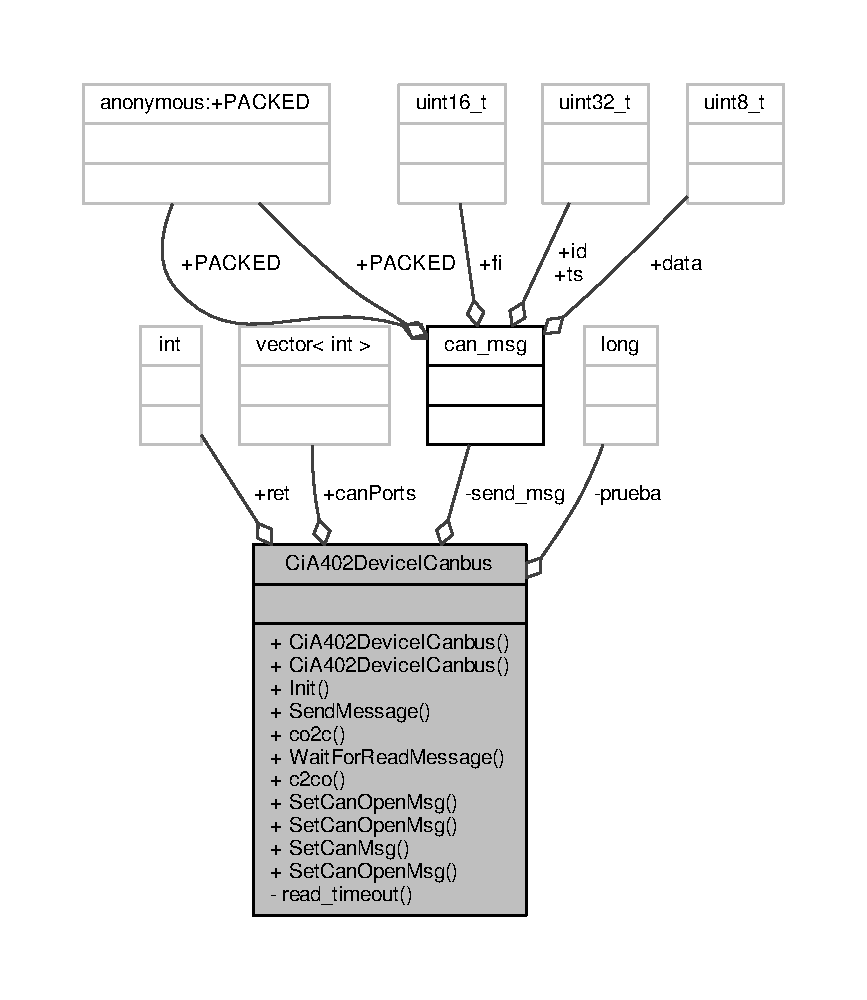
\includegraphics[width=350pt]{classCiA402DeviceICanbus__coll__graph}
\end{center}
\end{figure}
\subsection*{Public Member Functions}
\begin{DoxyCompactItemize}
\item 
\hyperlink{classCiA402DeviceICanbus_a557d59fe9c75dbdd0fc2cf2b3340e95a}{Ci\+A402\+Device\+I\+Canbus} ()
\item 
\hyperlink{classCiA402DeviceICanbus_a205b5105bd658b73b582cf1685f1d320}{Ci\+A402\+Device\+I\+Canbus} (long number, string can\+Port)
\item 
long \hyperlink{classCiA402DeviceICanbus_a757447054eadb6824cf779ca58d276ae}{Init} (const vector$<$ int $>$ \&new\+\_\+can\+Ports, string can\+Port)
\item 
int \hyperlink{classCiA402DeviceICanbus_ac831e319febc65d424955e32ecdf72c3}{Send\+Message} (\hyperlink{structco__msg}{co\+\_\+msg} input, unsigned int can\+Index)
\item 
long \hyperlink{classCiA402DeviceICanbus_aa108188c7f32a1c5d1f50662e66c6676}{co2c} (const \hyperlink{structco__msg}{co\+\_\+msg} \&input, \hyperlink{structcan__msg}{can\+\_\+msg} \&output)
\item 
int \hyperlink{classCiA402DeviceICanbus_a1f8d07b892461470a29ac5d30f3dd679}{Wait\+For\+Read\+Message} (\hyperlink{structco__msg}{co\+\_\+msg} \&output, unsigned int can\+Index)
\item 
long \hyperlink{classCiA402DeviceICanbus_aab504488399b2d5a5a010efef29e3d64}{c2co} (const \hyperlink{structcan__msg}{can\+\_\+msg} \&input, \hyperlink{structco__msg}{co\+\_\+msg} \&output)
\item 
int \hyperlink{classCiA402DeviceICanbus_aa439b9175f5879282058a3f4c2edb45d}{Set\+Can\+Open\+Msg} (\hyperlink{structco__msg}{co\+\_\+msg} \&msg\+\_\+co)
\item 
int \hyperlink{classCiA402DeviceICanbus_af09467b107e73f67804942db1597d983}{Set\+Can\+Open\+Msg} (\hyperlink{structco__msg}{co\+\_\+msg} \&msg\+\_\+co, uint8\+\_\+t msg\+\_\+start\mbox{[}$\,$\mbox{]})
\item 
\hyperlink{structcan__msg}{can\+\_\+msg} \hyperlink{classCiA402DeviceICanbus_a93cde3041c3d0a26666b451aa70b246f}{Set\+Can\+Msg} (\hyperlink{structcan__msg}{can\+\_\+msg} \&msg, uint8\+\_\+t msg\+\_\+start\mbox{[}$\,$\mbox{]})
\item 
\hyperlink{structco__msg}{co\+\_\+msg} \hyperlink{classCiA402DeviceICanbus_ab861fc4d62c917bdb1c06b886c8ed45a}{Set\+Can\+Open\+Msg} (unsigned short id\+\_\+co, unsigned short rtr, vector$<$ uint8\+\_\+t $>$ co\+Data\+Frame)
\begin{DoxyCompactList}\small\item\em \hyperlink{classCiA402DeviceICanbus_aa439b9175f5879282058a3f4c2edb45d}{Ci\+A402\+Device\+I\+Canbus\+::\+Set\+Can\+Open\+Msg} \+: Constructs canopen message from parameters. \end{DoxyCompactList}\end{DoxyCompactItemize}
\subsection*{Public Attributes}
\begin{DoxyCompactItemize}
\item 
vector$<$ int $>$ \hyperlink{classCiA402DeviceICanbus_a456534a394e4072025f2528938d1070d}{can\+Ports}
\item 
int \hyperlink{classCiA402DeviceICanbus_af6cf1493b669ce0415cefed7d84e5710}{ret}
\end{DoxyCompactItemize}
\subsection*{Private Member Functions}
\begin{DoxyCompactItemize}
\item 
int \hyperlink{classCiA402DeviceICanbus_a2ef5507ddae8411aae5b6e47e611ab92}{read\+\_\+timeout} (int fd, \hyperlink{structcan__msg}{can\+\_\+msg} $\ast$buf, unsigned int timeout)
\end{DoxyCompactItemize}
\subsection*{Private Attributes}
\begin{DoxyCompactItemize}
\item 
\hyperlink{structcan__msg}{can\+\_\+msg} \hyperlink{classCiA402DeviceICanbus_a47d8ee98f0f3569874a4018268ab1fb5}{send\+\_\+msg}
\item 
long \hyperlink{classCiA402DeviceICanbus_aa3ab38e7395ad35b3cc28281352b5e40}{prueba}
\end{DoxyCompactItemize}


\subsection{Constructor \& Destructor Documentation}
\index{Ci\+A402\+Device\+I\+Canbus@{Ci\+A402\+Device\+I\+Canbus}!Ci\+A402\+Device\+I\+Canbus@{Ci\+A402\+Device\+I\+Canbus}}
\index{Ci\+A402\+Device\+I\+Canbus@{Ci\+A402\+Device\+I\+Canbus}!Ci\+A402\+Device\+I\+Canbus@{Ci\+A402\+Device\+I\+Canbus}}
\subsubsection[{\texorpdfstring{Ci\+A402\+Device\+I\+Canbus()}{CiA402DeviceICanbus()}}]{\setlength{\rightskip}{0pt plus 5cm}Ci\+A402\+Device\+I\+Canbus\+::\+Ci\+A402\+Device\+I\+Canbus (
\begin{DoxyParamCaption}
{}
\end{DoxyParamCaption}
)}\hypertarget{classCiA402DeviceICanbus_a557d59fe9c75dbdd0fc2cf2b3340e95a}{}\label{classCiA402DeviceICanbus_a557d59fe9c75dbdd0fc2cf2b3340e95a}
\index{Ci\+A402\+Device\+I\+Canbus@{Ci\+A402\+Device\+I\+Canbus}!Ci\+A402\+Device\+I\+Canbus@{Ci\+A402\+Device\+I\+Canbus}}
\index{Ci\+A402\+Device\+I\+Canbus@{Ci\+A402\+Device\+I\+Canbus}!Ci\+A402\+Device\+I\+Canbus@{Ci\+A402\+Device\+I\+Canbus}}
\subsubsection[{\texorpdfstring{Ci\+A402\+Device\+I\+Canbus(long number, string can\+Port)}{CiA402DeviceICanbus(long number, string canPort)}}]{\setlength{\rightskip}{0pt plus 5cm}Ci\+A402\+Device\+I\+Canbus\+::\+Ci\+A402\+Device\+I\+Canbus (
\begin{DoxyParamCaption}
\item[{long}]{number, }
\item[{string}]{can\+Port}
\end{DoxyParamCaption}
)}\hypertarget{classCiA402DeviceICanbus_a205b5105bd658b73b582cf1685f1d320}{}\label{classCiA402DeviceICanbus_a205b5105bd658b73b582cf1685f1d320}


\subsection{Member Function Documentation}
\index{Ci\+A402\+Device\+I\+Canbus@{Ci\+A402\+Device\+I\+Canbus}!c2co@{c2co}}
\index{c2co@{c2co}!Ci\+A402\+Device\+I\+Canbus@{Ci\+A402\+Device\+I\+Canbus}}
\subsubsection[{\texorpdfstring{c2co(const can\+\_\+msg \&input, co\+\_\+msg \&output)}{c2co(const can_msg &input, co_msg &output)}}]{\setlength{\rightskip}{0pt plus 5cm}long Ci\+A402\+Device\+I\+Canbus\+::c2co (
\begin{DoxyParamCaption}
\item[{const {\bf can\+\_\+msg} \&}]{input, }
\item[{{\bf co\+\_\+msg} \&}]{output}
\end{DoxyParamCaption}
)}\hypertarget{classCiA402DeviceICanbus_aab504488399b2d5a5a010efef29e3d64}{}\label{classCiA402DeviceICanbus_aab504488399b2d5a5a010efef29e3d64}
\index{Ci\+A402\+Device\+I\+Canbus@{Ci\+A402\+Device\+I\+Canbus}!co2c@{co2c}}
\index{co2c@{co2c}!Ci\+A402\+Device\+I\+Canbus@{Ci\+A402\+Device\+I\+Canbus}}
\subsubsection[{\texorpdfstring{co2c(const co\+\_\+msg \&input, can\+\_\+msg \&output)}{co2c(const co_msg &input, can_msg &output)}}]{\setlength{\rightskip}{0pt plus 5cm}long Ci\+A402\+Device\+I\+Canbus\+::co2c (
\begin{DoxyParamCaption}
\item[{const {\bf co\+\_\+msg} \&}]{input, }
\item[{{\bf can\+\_\+msg} \&}]{output}
\end{DoxyParamCaption}
)}\hypertarget{classCiA402DeviceICanbus_aa108188c7f32a1c5d1f50662e66c6676}{}\label{classCiA402DeviceICanbus_aa108188c7f32a1c5d1f50662e66c6676}
\index{Ci\+A402\+Device\+I\+Canbus@{Ci\+A402\+Device\+I\+Canbus}!Init@{Init}}
\index{Init@{Init}!Ci\+A402\+Device\+I\+Canbus@{Ci\+A402\+Device\+I\+Canbus}}
\subsubsection[{\texorpdfstring{Init(const vector$<$ int $>$ \&new\+\_\+can\+Ports, string can\+Port)}{Init(const vector< int > &new_canPorts, string canPort)}}]{\setlength{\rightskip}{0pt plus 5cm}long Ci\+A402\+Device\+I\+Canbus\+::\+Init (
\begin{DoxyParamCaption}
\item[{const vector$<$ int $>$ \&}]{new\+\_\+can\+Ports, }
\item[{string}]{can\+Port}
\end{DoxyParamCaption}
)}\hypertarget{classCiA402DeviceICanbus_a757447054eadb6824cf779ca58d276ae}{}\label{classCiA402DeviceICanbus_a757447054eadb6824cf779ca58d276ae}
\index{Ci\+A402\+Device\+I\+Canbus@{Ci\+A402\+Device\+I\+Canbus}!read\+\_\+timeout@{read\+\_\+timeout}}
\index{read\+\_\+timeout@{read\+\_\+timeout}!Ci\+A402\+Device\+I\+Canbus@{Ci\+A402\+Device\+I\+Canbus}}
\subsubsection[{\texorpdfstring{read\+\_\+timeout(int fd, can\+\_\+msg $\ast$buf, unsigned int timeout)}{read_timeout(int fd, can_msg *buf, unsigned int timeout)}}]{\setlength{\rightskip}{0pt plus 5cm}int Ci\+A402\+Device\+I\+Canbus\+::read\+\_\+timeout (
\begin{DoxyParamCaption}
\item[{int}]{fd, }
\item[{{\bf can\+\_\+msg} $\ast$}]{buf, }
\item[{unsigned int}]{timeout}
\end{DoxyParamCaption}
)\hspace{0.3cm}{\ttfamily [private]}}\hypertarget{classCiA402DeviceICanbus_a2ef5507ddae8411aae5b6e47e611ab92}{}\label{classCiA402DeviceICanbus_a2ef5507ddae8411aae5b6e47e611ab92}
\index{Ci\+A402\+Device\+I\+Canbus@{Ci\+A402\+Device\+I\+Canbus}!Send\+Message@{Send\+Message}}
\index{Send\+Message@{Send\+Message}!Ci\+A402\+Device\+I\+Canbus@{Ci\+A402\+Device\+I\+Canbus}}
\subsubsection[{\texorpdfstring{Send\+Message(co\+\_\+msg input, unsigned int can\+Index)}{SendMessage(co_msg input, unsigned int canIndex)}}]{\setlength{\rightskip}{0pt plus 5cm}int Ci\+A402\+Device\+I\+Canbus\+::\+Send\+Message (
\begin{DoxyParamCaption}
\item[{{\bf co\+\_\+msg}}]{input, }
\item[{unsigned int}]{can\+Index}
\end{DoxyParamCaption}
)}\hypertarget{classCiA402DeviceICanbus_ac831e319febc65d424955e32ecdf72c3}{}\label{classCiA402DeviceICanbus_ac831e319febc65d424955e32ecdf72c3}
\index{Ci\+A402\+Device\+I\+Canbus@{Ci\+A402\+Device\+I\+Canbus}!Set\+Can\+Msg@{Set\+Can\+Msg}}
\index{Set\+Can\+Msg@{Set\+Can\+Msg}!Ci\+A402\+Device\+I\+Canbus@{Ci\+A402\+Device\+I\+Canbus}}
\subsubsection[{\texorpdfstring{Set\+Can\+Msg(can\+\_\+msg \&msg, uint8\+\_\+t msg\+\_\+start[])}{SetCanMsg(can_msg &msg, uint8_t msg_start[])}}]{\setlength{\rightskip}{0pt plus 5cm}{\bf can\+\_\+msg} Ci\+A402\+Device\+I\+Canbus\+::\+Set\+Can\+Msg (
\begin{DoxyParamCaption}
\item[{{\bf can\+\_\+msg} \&}]{msg, }
\item[{uint8\+\_\+t}]{msg\+\_\+start\mbox{[}$\,$\mbox{]}}
\end{DoxyParamCaption}
)}\hypertarget{classCiA402DeviceICanbus_a93cde3041c3d0a26666b451aa70b246f}{}\label{classCiA402DeviceICanbus_a93cde3041c3d0a26666b451aa70b246f}
\index{Ci\+A402\+Device\+I\+Canbus@{Ci\+A402\+Device\+I\+Canbus}!Set\+Can\+Open\+Msg@{Set\+Can\+Open\+Msg}}
\index{Set\+Can\+Open\+Msg@{Set\+Can\+Open\+Msg}!Ci\+A402\+Device\+I\+Canbus@{Ci\+A402\+Device\+I\+Canbus}}
\subsubsection[{\texorpdfstring{Set\+Can\+Open\+Msg(co\+\_\+msg \&msg\+\_\+co)}{SetCanOpenMsg(co_msg &msg_co)}}]{\setlength{\rightskip}{0pt plus 5cm}int Ci\+A402\+Device\+I\+Canbus\+::\+Set\+Can\+Open\+Msg (
\begin{DoxyParamCaption}
\item[{{\bf co\+\_\+msg} \&}]{msg\+\_\+co}
\end{DoxyParamCaption}
)}\hypertarget{classCiA402DeviceICanbus_aa439b9175f5879282058a3f4c2edb45d}{}\label{classCiA402DeviceICanbus_aa439b9175f5879282058a3f4c2edb45d}
\index{Ci\+A402\+Device\+I\+Canbus@{Ci\+A402\+Device\+I\+Canbus}!Set\+Can\+Open\+Msg@{Set\+Can\+Open\+Msg}}
\index{Set\+Can\+Open\+Msg@{Set\+Can\+Open\+Msg}!Ci\+A402\+Device\+I\+Canbus@{Ci\+A402\+Device\+I\+Canbus}}
\subsubsection[{\texorpdfstring{Set\+Can\+Open\+Msg(co\+\_\+msg \&msg\+\_\+co, uint8\+\_\+t msg\+\_\+start[])}{SetCanOpenMsg(co_msg &msg_co, uint8_t msg_start[])}}]{\setlength{\rightskip}{0pt plus 5cm}int Ci\+A402\+Device\+I\+Canbus\+::\+Set\+Can\+Open\+Msg (
\begin{DoxyParamCaption}
\item[{{\bf co\+\_\+msg} \&}]{msg\+\_\+co, }
\item[{uint8\+\_\+t}]{msg\+\_\+start\mbox{[}$\,$\mbox{]}}
\end{DoxyParamCaption}
)}\hypertarget{classCiA402DeviceICanbus_af09467b107e73f67804942db1597d983}{}\label{classCiA402DeviceICanbus_af09467b107e73f67804942db1597d983}
\index{Ci\+A402\+Device\+I\+Canbus@{Ci\+A402\+Device\+I\+Canbus}!Set\+Can\+Open\+Msg@{Set\+Can\+Open\+Msg}}
\index{Set\+Can\+Open\+Msg@{Set\+Can\+Open\+Msg}!Ci\+A402\+Device\+I\+Canbus@{Ci\+A402\+Device\+I\+Canbus}}
\subsubsection[{\texorpdfstring{Set\+Can\+Open\+Msg(unsigned short id\+\_\+co, unsigned short rtr, vector$<$ uint8\+\_\+t $>$ co\+Data\+Frame)}{SetCanOpenMsg(unsigned short id_co, unsigned short rtr, vector< uint8_t > coDataFrame)}}]{\setlength{\rightskip}{0pt plus 5cm}{\bf co\+\_\+msg} Ci\+A402\+Device\+I\+Canbus\+::\+Set\+Can\+Open\+Msg (
\begin{DoxyParamCaption}
\item[{unsigned short}]{id\+\_\+co, }
\item[{unsigned short}]{rtr, }
\item[{vector$<$ uint8\+\_\+t $>$}]{co\+Data\+Frame}
\end{DoxyParamCaption}
)}\hypertarget{classCiA402DeviceICanbus_ab861fc4d62c917bdb1c06b886c8ed45a}{}\label{classCiA402DeviceICanbus_ab861fc4d62c917bdb1c06b886c8ed45a}


\hyperlink{classCiA402DeviceICanbus_aa439b9175f5879282058a3f4c2edb45d}{Ci\+A402\+Device\+I\+Canbus\+::\+Set\+Can\+Open\+Msg} \+: Constructs canopen message from parameters. 


\begin{DoxyParams}{Parameters}
{\em id\+\_\+co} & cob id canopen parameter. \\
\hline
{\em rtr} & request for remote. \\
\hline
{\em msg\+\_\+start} & \+: canopen data frame. \\
\hline
\end{DoxyParams}
\begin{DoxyReturn}{Returns}
\+: canopen constructed message in \hyperlink{structco__msg}{co\+\_\+msg} data type. 
\end{DoxyReturn}
\index{Ci\+A402\+Device\+I\+Canbus@{Ci\+A402\+Device\+I\+Canbus}!Wait\+For\+Read\+Message@{Wait\+For\+Read\+Message}}
\index{Wait\+For\+Read\+Message@{Wait\+For\+Read\+Message}!Ci\+A402\+Device\+I\+Canbus@{Ci\+A402\+Device\+I\+Canbus}}
\subsubsection[{\texorpdfstring{Wait\+For\+Read\+Message(co\+\_\+msg \&output, unsigned int can\+Index)}{WaitForReadMessage(co_msg &output, unsigned int canIndex)}}]{\setlength{\rightskip}{0pt plus 5cm}int Ci\+A402\+Device\+I\+Canbus\+::\+Wait\+For\+Read\+Message (
\begin{DoxyParamCaption}
\item[{{\bf co\+\_\+msg} \&}]{output, }
\item[{unsigned int}]{can\+Index}
\end{DoxyParamCaption}
)}\hypertarget{classCiA402DeviceICanbus_a1f8d07b892461470a29ac5d30f3dd679}{}\label{classCiA402DeviceICanbus_a1f8d07b892461470a29ac5d30f3dd679}


\subsection{Member Data Documentation}
\index{Ci\+A402\+Device\+I\+Canbus@{Ci\+A402\+Device\+I\+Canbus}!can\+Ports@{can\+Ports}}
\index{can\+Ports@{can\+Ports}!Ci\+A402\+Device\+I\+Canbus@{Ci\+A402\+Device\+I\+Canbus}}
\subsubsection[{\texorpdfstring{can\+Ports}{canPorts}}]{\setlength{\rightskip}{0pt plus 5cm}vector$<$int$>$ Ci\+A402\+Device\+I\+Canbus\+::can\+Ports}\hypertarget{classCiA402DeviceICanbus_a456534a394e4072025f2528938d1070d}{}\label{classCiA402DeviceICanbus_a456534a394e4072025f2528938d1070d}
\index{Ci\+A402\+Device\+I\+Canbus@{Ci\+A402\+Device\+I\+Canbus}!prueba@{prueba}}
\index{prueba@{prueba}!Ci\+A402\+Device\+I\+Canbus@{Ci\+A402\+Device\+I\+Canbus}}
\subsubsection[{\texorpdfstring{prueba}{prueba}}]{\setlength{\rightskip}{0pt plus 5cm}long Ci\+A402\+Device\+I\+Canbus\+::prueba\hspace{0.3cm}{\ttfamily [private]}}\hypertarget{classCiA402DeviceICanbus_aa3ab38e7395ad35b3cc28281352b5e40}{}\label{classCiA402DeviceICanbus_aa3ab38e7395ad35b3cc28281352b5e40}
\index{Ci\+A402\+Device\+I\+Canbus@{Ci\+A402\+Device\+I\+Canbus}!ret@{ret}}
\index{ret@{ret}!Ci\+A402\+Device\+I\+Canbus@{Ci\+A402\+Device\+I\+Canbus}}
\subsubsection[{\texorpdfstring{ret}{ret}}]{\setlength{\rightskip}{0pt plus 5cm}int Ci\+A402\+Device\+I\+Canbus\+::ret}\hypertarget{classCiA402DeviceICanbus_af6cf1493b669ce0415cefed7d84e5710}{}\label{classCiA402DeviceICanbus_af6cf1493b669ce0415cefed7d84e5710}
\index{Ci\+A402\+Device\+I\+Canbus@{Ci\+A402\+Device\+I\+Canbus}!send\+\_\+msg@{send\+\_\+msg}}
\index{send\+\_\+msg@{send\+\_\+msg}!Ci\+A402\+Device\+I\+Canbus@{Ci\+A402\+Device\+I\+Canbus}}
\subsubsection[{\texorpdfstring{send\+\_\+msg}{send_msg}}]{\setlength{\rightskip}{0pt plus 5cm}{\bf can\+\_\+msg} Ci\+A402\+Device\+I\+Canbus\+::send\+\_\+msg\hspace{0.3cm}{\ttfamily [private]}}\hypertarget{classCiA402DeviceICanbus_a47d8ee98f0f3569874a4018268ab1fb5}{}\label{classCiA402DeviceICanbus_a47d8ee98f0f3569874a4018268ab1fb5}


The documentation for this class was generated from the following files\+:\begin{DoxyCompactItemize}
\item 
\hyperlink{CiA402DeviceICanbus_8h}{Ci\+A402\+Device\+I\+Canbus.\+h}\item 
\hyperlink{CiA402DeviceICanbus_8cpp}{Ci\+A402\+Device\+I\+Canbus.\+cpp}\end{DoxyCompactItemize}

\hypertarget{classCiA402SetupData}{}\section{Ci\+A402\+Setup\+Data Class Reference}
\label{classCiA402SetupData}\index{Ci\+A402\+Setup\+Data@{Ci\+A402\+Setup\+Data}}


{\ttfamily \#include $<$Ci\+A402\+Setup\+Data.\+h$>$}



Collaboration diagram for Ci\+A402\+Setup\+Data\+:
\nopagebreak
\begin{figure}[H]
\begin{center}
\leavevmode
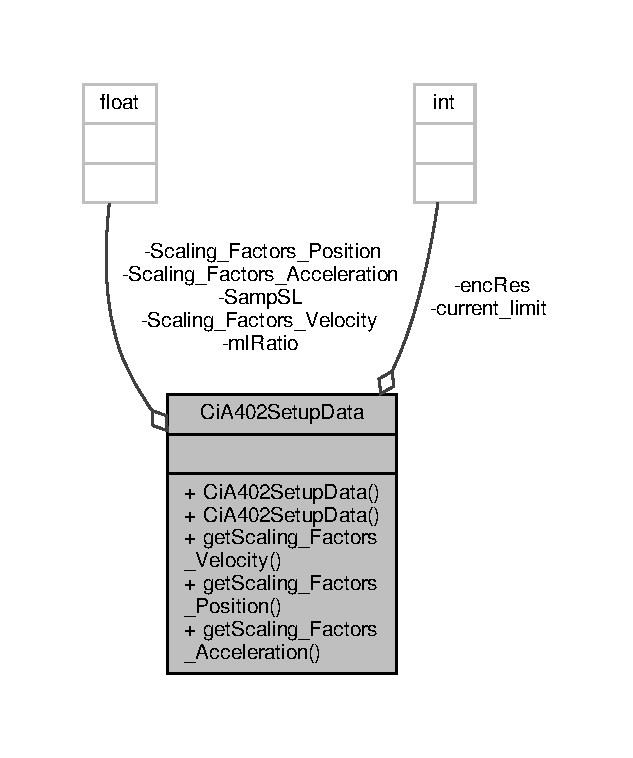
\includegraphics[width=304pt]{classCiA402SetupData__coll__graph}
\end{center}
\end{figure}
\subsection*{Public Member Functions}
\begin{DoxyCompactItemize}
\item 
\hyperlink{classCiA402SetupData_a75fda7c40eed83f736c227cf681bd0c5}{Ci\+A402\+Setup\+Data} ()
\item 
\hyperlink{classCiA402SetupData_ae7f96988b42fad6572e8227c5a6d1093}{Ci\+A402\+Setup\+Data} (int new\+\_\+enc\+Res, float new\+\_\+ml\+Ratio, float new\+\_\+\+Samp\+SL, int new\+\_\+current\+\_\+limit)
\item 
float \hyperlink{classCiA402SetupData_a97fa96f9f1fdc0b1367ef6b16e8974cf}{get\+Scaling\+\_\+\+Factors\+\_\+\+Velocity} () const 
\item 
float \hyperlink{classCiA402SetupData_afb42382bb460634c986f3e07a7fff583}{get\+Scaling\+\_\+\+Factors\+\_\+\+Position} () const 
\item 
float \hyperlink{classCiA402SetupData_aa1f8fb8d5a63b0a4dfa64051e98fa5e6}{get\+Scaling\+\_\+\+Factors\+\_\+\+Acceleration} () const 
\item 
int \hyperlink{classCiA402SetupData_a45e664d22fb598a8c267952ddbd7d1c3}{get\+Enc\+Res} () const 
\end{DoxyCompactItemize}
\subsection*{Private Attributes}
\begin{DoxyCompactItemize}
\item 
float \hyperlink{classCiA402SetupData_a35fc6c4d83a6b9cbb784532d75cf03b3}{ml\+Ratio}
\item 
int \hyperlink{classCiA402SetupData_a8d83cf7dce1f2aeaec2200c7567952b4}{enc\+Res}
\item 
float \hyperlink{classCiA402SetupData_a7dc6400c193ecfe21977437e7c5ac85f}{Samp\+SL}
\item 
int \hyperlink{classCiA402SetupData_a66da9919252d096f1190a70465dce20f}{current\+\_\+limit}
\item 
float \hyperlink{classCiA402SetupData_a1ac5a8bab56e6282f87684d4c7249225}{Scaling\+\_\+\+Factors\+\_\+\+Velocity}
\item 
float \hyperlink{classCiA402SetupData_a81ef1e6479ad92e748e33921dbf3cd25}{Scaling\+\_\+\+Factors\+\_\+\+Position}
\item 
float \hyperlink{classCiA402SetupData_afa253899425284c2fa62fdb678dc4907}{Scaling\+\_\+\+Factors\+\_\+\+Acceleration}
\end{DoxyCompactItemize}


\subsection{Constructor \& Destructor Documentation}
\index{Ci\+A402\+Setup\+Data@{Ci\+A402\+Setup\+Data}!Ci\+A402\+Setup\+Data@{Ci\+A402\+Setup\+Data}}
\index{Ci\+A402\+Setup\+Data@{Ci\+A402\+Setup\+Data}!Ci\+A402\+Setup\+Data@{Ci\+A402\+Setup\+Data}}
\subsubsection[{\texorpdfstring{Ci\+A402\+Setup\+Data()}{CiA402SetupData()}}]{\setlength{\rightskip}{0pt plus 5cm}Ci\+A402\+Setup\+Data\+::\+Ci\+A402\+Setup\+Data (
\begin{DoxyParamCaption}
{}
\end{DoxyParamCaption}
)}\hypertarget{classCiA402SetupData_a75fda7c40eed83f736c227cf681bd0c5}{}\label{classCiA402SetupData_a75fda7c40eed83f736c227cf681bd0c5}
\index{Ci\+A402\+Setup\+Data@{Ci\+A402\+Setup\+Data}!Ci\+A402\+Setup\+Data@{Ci\+A402\+Setup\+Data}}
\index{Ci\+A402\+Setup\+Data@{Ci\+A402\+Setup\+Data}!Ci\+A402\+Setup\+Data@{Ci\+A402\+Setup\+Data}}
\subsubsection[{\texorpdfstring{Ci\+A402\+Setup\+Data(int new\+\_\+enc\+Res, float new\+\_\+ml\+Ratio, float new\+\_\+\+Samp\+S\+L, int new\+\_\+current\+\_\+limit)}{CiA402SetupData(int new_encRes, float new_mlRatio, float new_SampSL, int new_current_limit)}}]{\setlength{\rightskip}{0pt plus 5cm}Ci\+A402\+Setup\+Data\+::\+Ci\+A402\+Setup\+Data (
\begin{DoxyParamCaption}
\item[{int}]{new\+\_\+enc\+Res, }
\item[{float}]{new\+\_\+ml\+Ratio, }
\item[{float}]{new\+\_\+\+Samp\+SL, }
\item[{int}]{new\+\_\+current\+\_\+limit}
\end{DoxyParamCaption}
)}\hypertarget{classCiA402SetupData_ae7f96988b42fad6572e8227c5a6d1093}{}\label{classCiA402SetupData_ae7f96988b42fad6572e8227c5a6d1093}


\subsection{Member Function Documentation}
\index{Ci\+A402\+Setup\+Data@{Ci\+A402\+Setup\+Data}!get\+Enc\+Res@{get\+Enc\+Res}}
\index{get\+Enc\+Res@{get\+Enc\+Res}!Ci\+A402\+Setup\+Data@{Ci\+A402\+Setup\+Data}}
\subsubsection[{\texorpdfstring{get\+Enc\+Res() const }{getEncRes() const }}]{\setlength{\rightskip}{0pt plus 5cm}int Ci\+A402\+Setup\+Data\+::get\+Enc\+Res (
\begin{DoxyParamCaption}
{}
\end{DoxyParamCaption}
) const}\hypertarget{classCiA402SetupData_a45e664d22fb598a8c267952ddbd7d1c3}{}\label{classCiA402SetupData_a45e664d22fb598a8c267952ddbd7d1c3}
\index{Ci\+A402\+Setup\+Data@{Ci\+A402\+Setup\+Data}!get\+Scaling\+\_\+\+Factors\+\_\+\+Acceleration@{get\+Scaling\+\_\+\+Factors\+\_\+\+Acceleration}}
\index{get\+Scaling\+\_\+\+Factors\+\_\+\+Acceleration@{get\+Scaling\+\_\+\+Factors\+\_\+\+Acceleration}!Ci\+A402\+Setup\+Data@{Ci\+A402\+Setup\+Data}}
\subsubsection[{\texorpdfstring{get\+Scaling\+\_\+\+Factors\+\_\+\+Acceleration() const }{getScaling_Factors_Acceleration() const }}]{\setlength{\rightskip}{0pt plus 5cm}float Ci\+A402\+Setup\+Data\+::get\+Scaling\+\_\+\+Factors\+\_\+\+Acceleration (
\begin{DoxyParamCaption}
{}
\end{DoxyParamCaption}
) const}\hypertarget{classCiA402SetupData_aa1f8fb8d5a63b0a4dfa64051e98fa5e6}{}\label{classCiA402SetupData_aa1f8fb8d5a63b0a4dfa64051e98fa5e6}
\index{Ci\+A402\+Setup\+Data@{Ci\+A402\+Setup\+Data}!get\+Scaling\+\_\+\+Factors\+\_\+\+Position@{get\+Scaling\+\_\+\+Factors\+\_\+\+Position}}
\index{get\+Scaling\+\_\+\+Factors\+\_\+\+Position@{get\+Scaling\+\_\+\+Factors\+\_\+\+Position}!Ci\+A402\+Setup\+Data@{Ci\+A402\+Setup\+Data}}
\subsubsection[{\texorpdfstring{get\+Scaling\+\_\+\+Factors\+\_\+\+Position() const }{getScaling_Factors_Position() const }}]{\setlength{\rightskip}{0pt plus 5cm}float Ci\+A402\+Setup\+Data\+::get\+Scaling\+\_\+\+Factors\+\_\+\+Position (
\begin{DoxyParamCaption}
{}
\end{DoxyParamCaption}
) const}\hypertarget{classCiA402SetupData_afb42382bb460634c986f3e07a7fff583}{}\label{classCiA402SetupData_afb42382bb460634c986f3e07a7fff583}
\index{Ci\+A402\+Setup\+Data@{Ci\+A402\+Setup\+Data}!get\+Scaling\+\_\+\+Factors\+\_\+\+Velocity@{get\+Scaling\+\_\+\+Factors\+\_\+\+Velocity}}
\index{get\+Scaling\+\_\+\+Factors\+\_\+\+Velocity@{get\+Scaling\+\_\+\+Factors\+\_\+\+Velocity}!Ci\+A402\+Setup\+Data@{Ci\+A402\+Setup\+Data}}
\subsubsection[{\texorpdfstring{get\+Scaling\+\_\+\+Factors\+\_\+\+Velocity() const }{getScaling_Factors_Velocity() const }}]{\setlength{\rightskip}{0pt plus 5cm}float Ci\+A402\+Setup\+Data\+::get\+Scaling\+\_\+\+Factors\+\_\+\+Velocity (
\begin{DoxyParamCaption}
{}
\end{DoxyParamCaption}
) const}\hypertarget{classCiA402SetupData_a97fa96f9f1fdc0b1367ef6b16e8974cf}{}\label{classCiA402SetupData_a97fa96f9f1fdc0b1367ef6b16e8974cf}


\subsection{Member Data Documentation}
\index{Ci\+A402\+Setup\+Data@{Ci\+A402\+Setup\+Data}!current\+\_\+limit@{current\+\_\+limit}}
\index{current\+\_\+limit@{current\+\_\+limit}!Ci\+A402\+Setup\+Data@{Ci\+A402\+Setup\+Data}}
\subsubsection[{\texorpdfstring{current\+\_\+limit}{current_limit}}]{\setlength{\rightskip}{0pt plus 5cm}int Ci\+A402\+Setup\+Data\+::current\+\_\+limit\hspace{0.3cm}{\ttfamily [private]}}\hypertarget{classCiA402SetupData_a66da9919252d096f1190a70465dce20f}{}\label{classCiA402SetupData_a66da9919252d096f1190a70465dce20f}
\index{Ci\+A402\+Setup\+Data@{Ci\+A402\+Setup\+Data}!enc\+Res@{enc\+Res}}
\index{enc\+Res@{enc\+Res}!Ci\+A402\+Setup\+Data@{Ci\+A402\+Setup\+Data}}
\subsubsection[{\texorpdfstring{enc\+Res}{encRes}}]{\setlength{\rightskip}{0pt plus 5cm}int Ci\+A402\+Setup\+Data\+::enc\+Res\hspace{0.3cm}{\ttfamily [private]}}\hypertarget{classCiA402SetupData_a8d83cf7dce1f2aeaec2200c7567952b4}{}\label{classCiA402SetupData_a8d83cf7dce1f2aeaec2200c7567952b4}
\index{Ci\+A402\+Setup\+Data@{Ci\+A402\+Setup\+Data}!ml\+Ratio@{ml\+Ratio}}
\index{ml\+Ratio@{ml\+Ratio}!Ci\+A402\+Setup\+Data@{Ci\+A402\+Setup\+Data}}
\subsubsection[{\texorpdfstring{ml\+Ratio}{mlRatio}}]{\setlength{\rightskip}{0pt plus 5cm}float Ci\+A402\+Setup\+Data\+::ml\+Ratio\hspace{0.3cm}{\ttfamily [private]}}\hypertarget{classCiA402SetupData_a35fc6c4d83a6b9cbb784532d75cf03b3}{}\label{classCiA402SetupData_a35fc6c4d83a6b9cbb784532d75cf03b3}
\index{Ci\+A402\+Setup\+Data@{Ci\+A402\+Setup\+Data}!Samp\+SL@{Samp\+SL}}
\index{Samp\+SL@{Samp\+SL}!Ci\+A402\+Setup\+Data@{Ci\+A402\+Setup\+Data}}
\subsubsection[{\texorpdfstring{Samp\+SL}{SampSL}}]{\setlength{\rightskip}{0pt plus 5cm}float Ci\+A402\+Setup\+Data\+::\+Samp\+SL\hspace{0.3cm}{\ttfamily [private]}}\hypertarget{classCiA402SetupData_a7dc6400c193ecfe21977437e7c5ac85f}{}\label{classCiA402SetupData_a7dc6400c193ecfe21977437e7c5ac85f}
\index{Ci\+A402\+Setup\+Data@{Ci\+A402\+Setup\+Data}!Scaling\+\_\+\+Factors\+\_\+\+Acceleration@{Scaling\+\_\+\+Factors\+\_\+\+Acceleration}}
\index{Scaling\+\_\+\+Factors\+\_\+\+Acceleration@{Scaling\+\_\+\+Factors\+\_\+\+Acceleration}!Ci\+A402\+Setup\+Data@{Ci\+A402\+Setup\+Data}}
\subsubsection[{\texorpdfstring{Scaling\+\_\+\+Factors\+\_\+\+Acceleration}{Scaling_Factors_Acceleration}}]{\setlength{\rightskip}{0pt plus 5cm}float Ci\+A402\+Setup\+Data\+::\+Scaling\+\_\+\+Factors\+\_\+\+Acceleration\hspace{0.3cm}{\ttfamily [private]}}\hypertarget{classCiA402SetupData_afa253899425284c2fa62fdb678dc4907}{}\label{classCiA402SetupData_afa253899425284c2fa62fdb678dc4907}
\index{Ci\+A402\+Setup\+Data@{Ci\+A402\+Setup\+Data}!Scaling\+\_\+\+Factors\+\_\+\+Position@{Scaling\+\_\+\+Factors\+\_\+\+Position}}
\index{Scaling\+\_\+\+Factors\+\_\+\+Position@{Scaling\+\_\+\+Factors\+\_\+\+Position}!Ci\+A402\+Setup\+Data@{Ci\+A402\+Setup\+Data}}
\subsubsection[{\texorpdfstring{Scaling\+\_\+\+Factors\+\_\+\+Position}{Scaling_Factors_Position}}]{\setlength{\rightskip}{0pt plus 5cm}float Ci\+A402\+Setup\+Data\+::\+Scaling\+\_\+\+Factors\+\_\+\+Position\hspace{0.3cm}{\ttfamily [private]}}\hypertarget{classCiA402SetupData_a81ef1e6479ad92e748e33921dbf3cd25}{}\label{classCiA402SetupData_a81ef1e6479ad92e748e33921dbf3cd25}
\index{Ci\+A402\+Setup\+Data@{Ci\+A402\+Setup\+Data}!Scaling\+\_\+\+Factors\+\_\+\+Velocity@{Scaling\+\_\+\+Factors\+\_\+\+Velocity}}
\index{Scaling\+\_\+\+Factors\+\_\+\+Velocity@{Scaling\+\_\+\+Factors\+\_\+\+Velocity}!Ci\+A402\+Setup\+Data@{Ci\+A402\+Setup\+Data}}
\subsubsection[{\texorpdfstring{Scaling\+\_\+\+Factors\+\_\+\+Velocity}{Scaling_Factors_Velocity}}]{\setlength{\rightskip}{0pt plus 5cm}float Ci\+A402\+Setup\+Data\+::\+Scaling\+\_\+\+Factors\+\_\+\+Velocity\hspace{0.3cm}{\ttfamily [private]}}\hypertarget{classCiA402SetupData_a1ac5a8bab56e6282f87684d4c7249225}{}\label{classCiA402SetupData_a1ac5a8bab56e6282f87684d4c7249225}


The documentation for this class was generated from the following files\+:\begin{DoxyCompactItemize}
\item 
\hyperlink{CiA402SetupData_8h}{Ci\+A402\+Setup\+Data.\+h}\item 
\hyperlink{CiA402SetupData_8cpp}{Ci\+A402\+Setup\+Data.\+cpp}\end{DoxyCompactItemize}

\hypertarget{structco__msg}{}\section{co\+\_\+msg Struct Reference}
\label{structco__msg}\index{co\+\_\+msg@{co\+\_\+msg}}


{\ttfamily \#include $<$candatatypes.\+h$>$}



Collaboration diagram for co\+\_\+msg\+:\nopagebreak
\begin{figure}[H]
\begin{center}
\leavevmode
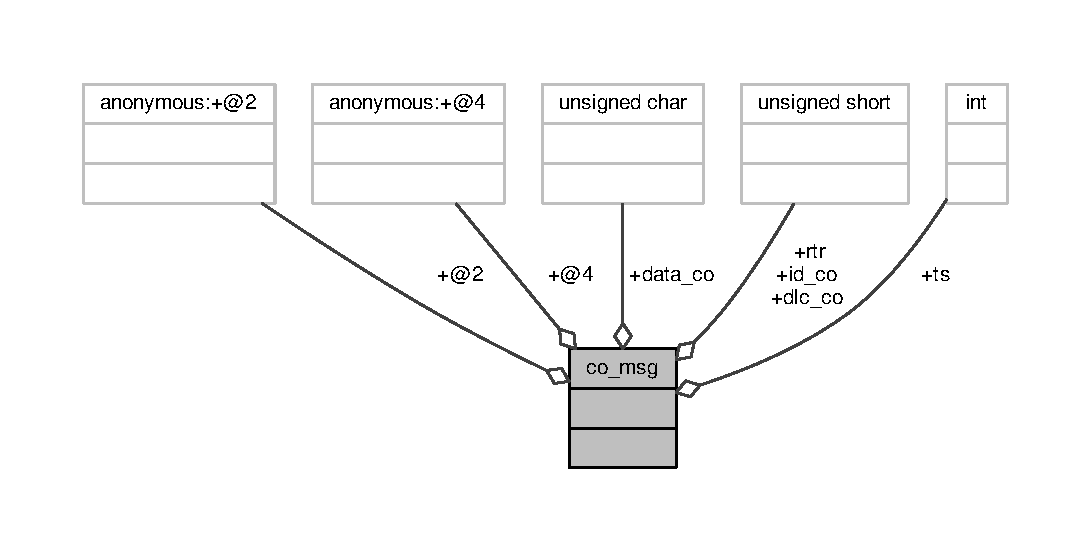
\includegraphics[width=350pt]{structco__msg__coll__graph}
\end{center}
\end{figure}
\subsection*{Public Attributes}
\begin{DoxyCompactItemize}
\item 
\begin{tabbing}
xx\=xx\=xx\=xx\=xx\=xx\=xx\=xx\=xx\=\kill
union \{\\
\>unsigned short \hyperlink{structco__msg_a634de83979d7da90565eccdf16304a07}{id\_co}\\
\}; \\

\end{tabbing}\item 
unsigned int \hyperlink{structco__msg_aaf8cd43d17baf495c982c87866fc90b2}{ts}
\item 
unsigned short \hyperlink{structco__msg_a4352880745fa6bc63d6c4e3c77870029}{rtr}\+:1
\item 
unsigned short \hyperlink{structco__msg_ab19d6996baf97d346427d9789d7e4a6b}{dlc\+\_\+co}
\item 
unsigned char \hyperlink{structco__msg_a3ced1bf4d72ca82fe53c829d42cd946e}{data\+\_\+co} \mbox{[}8\mbox{]}
\item 
\begin{tabbing}
xx\=xx\=xx\=xx\=xx\=xx\=xx\=xx\=xx\=\kill
union \{\\
\>unsigned short \hyperlink{structco__msg_a634de83979d7da90565eccdf16304a07}{id\_co}\\
\}; \\

\end{tabbing}\end{DoxyCompactItemize}


\subsection{Member Data Documentation}
\subsubsection[{\texorpdfstring{"@2}{@2}}]{\setlength{\rightskip}{0pt plus 5cm}union \{ ... \} }\hypertarget{structco__msg_af8251e2eaf9e807267d3ced55e292142}{}\label{structco__msg_af8251e2eaf9e807267d3ced55e292142}
\subsubsection[{\texorpdfstring{"@4}{@4}}]{\setlength{\rightskip}{0pt plus 5cm}union \{ ... \} }\hypertarget{structco__msg_a549464c55b7bbab6345f082dab73b275}{}\label{structco__msg_a549464c55b7bbab6345f082dab73b275}
\index{co\+\_\+msg@{co\+\_\+msg}!data\+\_\+co@{data\+\_\+co}}
\index{data\+\_\+co@{data\+\_\+co}!co\+\_\+msg@{co\+\_\+msg}}
\subsubsection[{\texorpdfstring{data\+\_\+co}{data_co}}]{\setlength{\rightskip}{0pt plus 5cm}unsigned char co\+\_\+msg\+::data\+\_\+co}\hypertarget{structco__msg_a3ced1bf4d72ca82fe53c829d42cd946e}{}\label{structco__msg_a3ced1bf4d72ca82fe53c829d42cd946e}
\index{co\+\_\+msg@{co\+\_\+msg}!dlc\+\_\+co@{dlc\+\_\+co}}
\index{dlc\+\_\+co@{dlc\+\_\+co}!co\+\_\+msg@{co\+\_\+msg}}
\subsubsection[{\texorpdfstring{dlc\+\_\+co}{dlc_co}}]{\setlength{\rightskip}{0pt plus 5cm}unsigned short co\+\_\+msg\+::dlc\+\_\+co}\hypertarget{structco__msg_ab19d6996baf97d346427d9789d7e4a6b}{}\label{structco__msg_ab19d6996baf97d346427d9789d7e4a6b}
\index{co\+\_\+msg@{co\+\_\+msg}!id\+\_\+co@{id\+\_\+co}}
\index{id\+\_\+co@{id\+\_\+co}!co\+\_\+msg@{co\+\_\+msg}}
\subsubsection[{\texorpdfstring{id\+\_\+co}{id_co}}]{\setlength{\rightskip}{0pt plus 5cm}unsigned short co\+\_\+msg\+::id\+\_\+co}\hypertarget{structco__msg_a634de83979d7da90565eccdf16304a07}{}\label{structco__msg_a634de83979d7da90565eccdf16304a07}
\index{co\+\_\+msg@{co\+\_\+msg}!rtr@{rtr}}
\index{rtr@{rtr}!co\+\_\+msg@{co\+\_\+msg}}
\subsubsection[{\texorpdfstring{rtr}{rtr}}]{\setlength{\rightskip}{0pt plus 5cm}unsigned short co\+\_\+msg\+::rtr}\hypertarget{structco__msg_a4352880745fa6bc63d6c4e3c77870029}{}\label{structco__msg_a4352880745fa6bc63d6c4e3c77870029}
\index{co\+\_\+msg@{co\+\_\+msg}!ts@{ts}}
\index{ts@{ts}!co\+\_\+msg@{co\+\_\+msg}}
\subsubsection[{\texorpdfstring{ts}{ts}}]{\setlength{\rightskip}{0pt plus 5cm}unsigned int co\+\_\+msg\+::ts}\hypertarget{structco__msg_aaf8cd43d17baf495c982c87866fc90b2}{}\label{structco__msg_aaf8cd43d17baf495c982c87866fc90b2}


The documentation for this struct was generated from the following files\+:\begin{DoxyCompactItemize}
\item 
\hyperlink{candatatypes_8h}{candatatypes.\+h}\item 
\hyperlink{co__msg_8h}{co\+\_\+msg.\+h}\end{DoxyCompactItemize}

\hypertarget{classDeviceChain}{}\section{Device\+Chain Class Reference}
\label{classDeviceChain}\index{Device\+Chain@{Device\+Chain}}


{\ttfamily \#include $<$Device\+Chain.\+h$>$}



Collaboration diagram for Device\+Chain\+:\nopagebreak
\begin{figure}[H]
\begin{center}
\leavevmode
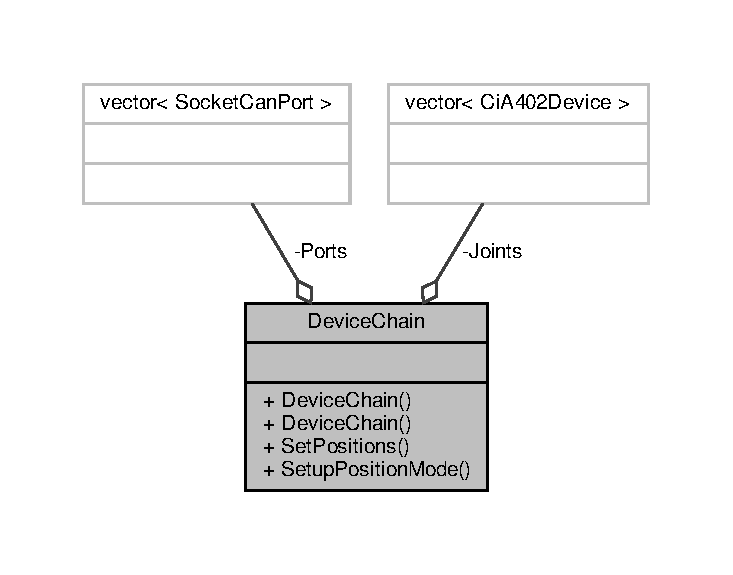
\includegraphics[width=350pt]{classDeviceChain__coll__graph}
\end{center}
\end{figure}
\subsection*{Public Member Functions}
\begin{DoxyCompactItemize}
\item 
\hyperlink{classDeviceChain_ad89af127eec501ad00ad5f5de197b21e}{Device\+Chain} (string actual\+Port)
\item 
\hyperlink{classDeviceChain_a20dd5853f160cfc8ef21ed93dac96f11}{Device\+Chain} (string actual\+Port, vector$<$ long $>$ ids)
\item 
long \hyperlink{classDeviceChain_ae6e9be5bfb46721d4c6b66d3d9541f25}{Set\+Positions} (vector$<$ double $>$ joint\+Angles)
\item 
long \hyperlink{classDeviceChain_a329b622f12a419f01a9bab38f869144b}{Setup\+Position\+Mode} (const uint32\+\_\+t velocity, const uint32\+\_\+t acceleration)
\end{DoxyCompactItemize}
\subsection*{Private Attributes}
\begin{DoxyCompactItemize}
\item 
std\+::vector$<$ \hyperlink{classCiA402Device}{Ci\+A402\+Device} $>$ \hyperlink{classDeviceChain_a114bea9dc1166ab2ea5a9ef7488c66ab}{Joints}
\item 
std\+::vector$<$ \hyperlink{classSocketCanPort}{Socket\+Can\+Port} $>$ \hyperlink{classDeviceChain_a760e12bf0095431fe76563cc5d7969de}{Ports}
\end{DoxyCompactItemize}


\subsection{Constructor \& Destructor Documentation}
\index{Device\+Chain@{Device\+Chain}!Device\+Chain@{Device\+Chain}}
\index{Device\+Chain@{Device\+Chain}!Device\+Chain@{Device\+Chain}}
\subsubsection[{\texorpdfstring{Device\+Chain(string actual\+Port)}{DeviceChain(string actualPort)}}]{\setlength{\rightskip}{0pt plus 5cm}Device\+Chain\+::\+Device\+Chain (
\begin{DoxyParamCaption}
\item[{string}]{actual\+Port}
\end{DoxyParamCaption}
)}\hypertarget{classDeviceChain_ad89af127eec501ad00ad5f5de197b21e}{}\label{classDeviceChain_ad89af127eec501ad00ad5f5de197b21e}
\index{Device\+Chain@{Device\+Chain}!Device\+Chain@{Device\+Chain}}
\index{Device\+Chain@{Device\+Chain}!Device\+Chain@{Device\+Chain}}
\subsubsection[{\texorpdfstring{Device\+Chain(string actual\+Port, vector$<$ long $>$ ids)}{DeviceChain(string actualPort, vector< long > ids)}}]{\setlength{\rightskip}{0pt plus 5cm}Device\+Chain\+::\+Device\+Chain (
\begin{DoxyParamCaption}
\item[{string}]{actual\+Port, }
\item[{vector$<$ long $>$}]{ids}
\end{DoxyParamCaption}
)}\hypertarget{classDeviceChain_a20dd5853f160cfc8ef21ed93dac96f11}{}\label{classDeviceChain_a20dd5853f160cfc8ef21ed93dac96f11}


\subsection{Member Function Documentation}
\index{Device\+Chain@{Device\+Chain}!Set\+Positions@{Set\+Positions}}
\index{Set\+Positions@{Set\+Positions}!Device\+Chain@{Device\+Chain}}
\subsubsection[{\texorpdfstring{Set\+Positions(vector$<$ double $>$ joint\+Angles)}{SetPositions(vector< double > jointAngles)}}]{\setlength{\rightskip}{0pt plus 5cm}long Device\+Chain\+::\+Set\+Positions (
\begin{DoxyParamCaption}
\item[{vector$<$ double $>$}]{joint\+Angles}
\end{DoxyParamCaption}
)}\hypertarget{classDeviceChain_ae6e9be5bfb46721d4c6b66d3d9541f25}{}\label{classDeviceChain_ae6e9be5bfb46721d4c6b66d3d9541f25}
\index{Device\+Chain@{Device\+Chain}!Setup\+Position\+Mode@{Setup\+Position\+Mode}}
\index{Setup\+Position\+Mode@{Setup\+Position\+Mode}!Device\+Chain@{Device\+Chain}}
\subsubsection[{\texorpdfstring{Setup\+Position\+Mode(const uint32\+\_\+t velocity, const uint32\+\_\+t acceleration)}{SetupPositionMode(const uint32_t velocity, const uint32_t acceleration)}}]{\setlength{\rightskip}{0pt plus 5cm}long Device\+Chain\+::\+Setup\+Position\+Mode (
\begin{DoxyParamCaption}
\item[{const uint32\+\_\+t}]{velocity, }
\item[{const uint32\+\_\+t}]{acceleration}
\end{DoxyParamCaption}
)}\hypertarget{classDeviceChain_a329b622f12a419f01a9bab38f869144b}{}\label{classDeviceChain_a329b622f12a419f01a9bab38f869144b}


\subsection{Member Data Documentation}
\index{Device\+Chain@{Device\+Chain}!Joints@{Joints}}
\index{Joints@{Joints}!Device\+Chain@{Device\+Chain}}
\subsubsection[{\texorpdfstring{Joints}{Joints}}]{\setlength{\rightskip}{0pt plus 5cm}std\+::vector$<${\bf Ci\+A402\+Device}$>$ Device\+Chain\+::\+Joints\hspace{0.3cm}{\ttfamily [private]}}\hypertarget{classDeviceChain_a114bea9dc1166ab2ea5a9ef7488c66ab}{}\label{classDeviceChain_a114bea9dc1166ab2ea5a9ef7488c66ab}
\index{Device\+Chain@{Device\+Chain}!Ports@{Ports}}
\index{Ports@{Ports}!Device\+Chain@{Device\+Chain}}
\subsubsection[{\texorpdfstring{Ports}{Ports}}]{\setlength{\rightskip}{0pt plus 5cm}std\+::vector$<${\bf Socket\+Can\+Port}$>$ Device\+Chain\+::\+Ports\hspace{0.3cm}{\ttfamily [private]}}\hypertarget{classDeviceChain_a760e12bf0095431fe76563cc5d7969de}{}\label{classDeviceChain_a760e12bf0095431fe76563cc5d7969de}


The documentation for this class was generated from the following files\+:\begin{DoxyCompactItemize}
\item 
\hyperlink{DeviceChain_8h}{Device\+Chain.\+h}\item 
\hyperlink{DeviceChain_8cpp}{Device\+Chain.\+cpp}\end{DoxyCompactItemize}

\hypertarget{structerr__stat}{}\section{err\+\_\+stat Struct Reference}
\label{structerr__stat}\index{err\+\_\+stat@{err\+\_\+stat}}


{\ttfamily \#include $<$hico\+\_\+api.\+h$>$}



Collaboration diagram for err\+\_\+stat\+:\nopagebreak
\begin{figure}[H]
\begin{center}
\leavevmode
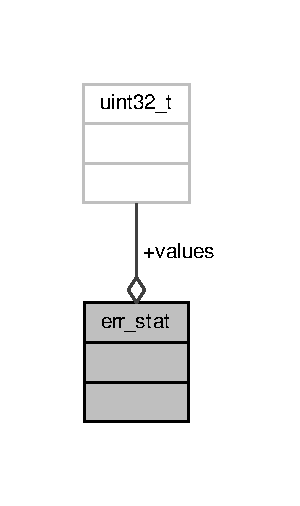
\includegraphics[width=144pt]{structerr__stat__coll__graph}
\end{center}
\end{figure}
\subsection*{Public Attributes}
\begin{DoxyCompactItemize}
\item 
uint32\+\_\+t \hyperlink{structerr__stat_a659e627af5963248da109c8e2404cd08}{values} \mbox{[}0x3f\mbox{]}
\end{DoxyCompactItemize}


\subsection{Member Data Documentation}
\index{err\+\_\+stat@{err\+\_\+stat}!values@{values}}
\index{values@{values}!err\+\_\+stat@{err\+\_\+stat}}
\subsubsection[{\texorpdfstring{values}{values}}]{\setlength{\rightskip}{0pt plus 5cm}uint32\+\_\+t err\+\_\+stat\+::values\mbox{[}0x3f\mbox{]}}\hypertarget{structerr__stat_a659e627af5963248da109c8e2404cd08}{}\label{structerr__stat_a659e627af5963248da109c8e2404cd08}


The documentation for this struct was generated from the following file\+:\begin{DoxyCompactItemize}
\item 
\hyperlink{hico__api_8h}{hico\+\_\+api.\+h}\end{DoxyCompactItemize}

\hypertarget{classPortBase}{}\section{Port\+Base Class Reference}
\label{classPortBase}\index{Port\+Base@{Port\+Base}}


{\ttfamily \#include $<$Port\+Base.\+h$>$}



Inheritance diagram for Port\+Base\+:
\nopagebreak
\begin{figure}[H]
\begin{center}
\leavevmode
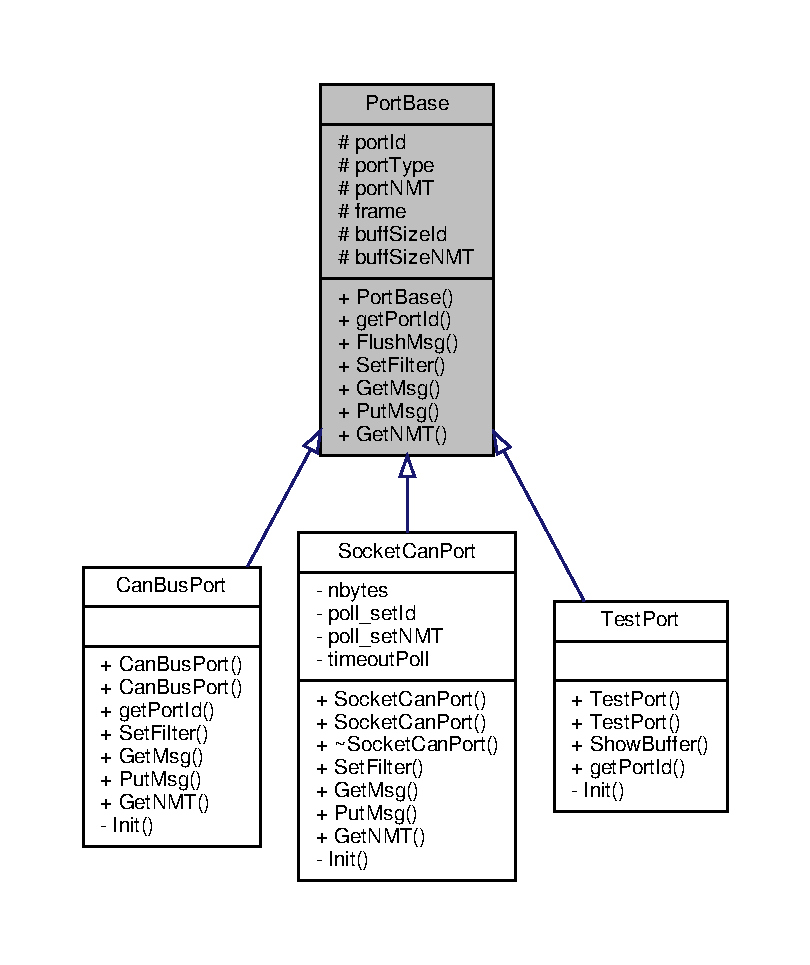
\includegraphics[width=350pt]{classPortBase__inherit__graph}
\end{center}
\end{figure}


Collaboration diagram for Port\+Base\+:
\nopagebreak
\begin{figure}[H]
\begin{center}
\leavevmode
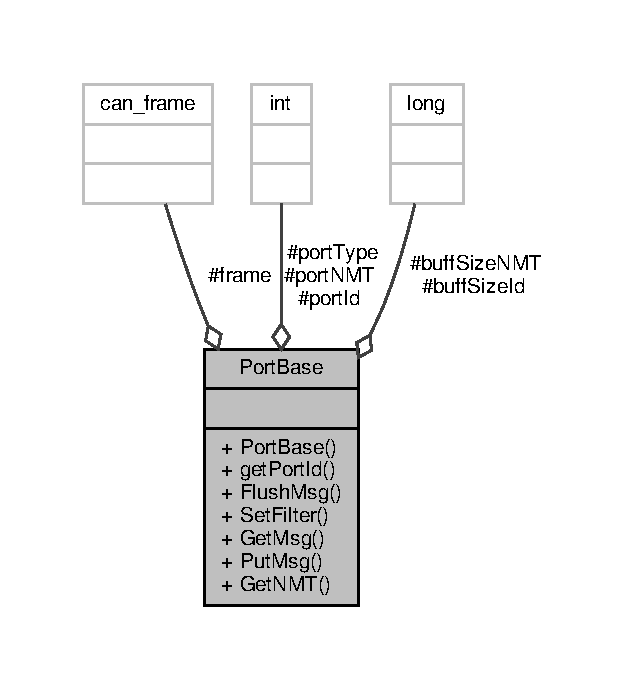
\includegraphics[width=301pt]{classPortBase__coll__graph}
\end{center}
\end{figure}
\subsection*{Public Member Functions}
\begin{DoxyCompactItemize}
\item 
\hyperlink{classPortBase_acb7872550bc94538ef95d2510d763be3}{Port\+Base} ()
\item 
int \hyperlink{classPortBase_a45ec4a2cd5e17e098f6f72677437f066}{get\+Port\+Id} ()
\item 
long \hyperlink{classPortBase_a913932fc850e9aebc947542773c669ad}{Flush\+Msg} ()
\item 
virtual long \hyperlink{classPortBase_a1d857a81a8e3f3bd460ef7c802ee762c}{Set\+Filter} (uint32\+\_\+t can\+Id, uint32\+\_\+t mask)=0
\item 
virtual long \hyperlink{classPortBase_a4fe82768f2b79889d7084292ac0e8696}{Get\+Msg} (uint32\+\_\+t \&can\+Id, uint8\+\_\+t $\ast$data, uint8\+\_\+t \&size)=0
\item 
virtual long \hyperlink{classPortBase_a26213ebb6ea0a0b77f60c28944e3bb8e}{Put\+Msg} (const uint32\+\_\+t \&can\+Id, uint8\+\_\+t $\ast$const data, const uint8\+\_\+t size)=0
\item 
virtual long \hyperlink{classPortBase_abab2bf17b01d87c2bca01cb2151aa2f1}{Get\+N\+MT} (uint8\+\_\+t $\ast$data, uint8\+\_\+t \&size)=0
\end{DoxyCompactItemize}
\subsection*{Protected Attributes}
\begin{DoxyCompactItemize}
\item 
int \hyperlink{classPortBase_af8816a6f73bf391d2948f3564f8ea1df}{port\+Id}
\item 
int \hyperlink{classPortBase_a6f18d480ef41a91fd2957927fe94c408}{port\+Type}
\item 
int \hyperlink{classPortBase_ae63f6df54bbeac1046b5dfbe178e1cee}{port\+N\+MT}
\item 
can\+\_\+frame \hyperlink{classPortBase_ae175156fa18f3be1820adea89ef7b13c}{frame}
\item 
long \hyperlink{classPortBase_a559431268076ea9b23bce545510f7b39}{buff\+Size\+Id}
\item 
long \hyperlink{classPortBase_aba8241e5d55c06c7d1a11ebb18096328}{buff\+Size\+N\+MT}
\end{DoxyCompactItemize}


\subsection{Constructor \& Destructor Documentation}
\index{Port\+Base@{Port\+Base}!Port\+Base@{Port\+Base}}
\index{Port\+Base@{Port\+Base}!Port\+Base@{Port\+Base}}
\subsubsection[{\texorpdfstring{Port\+Base()}{PortBase()}}]{\setlength{\rightskip}{0pt plus 5cm}Port\+Base\+::\+Port\+Base (
\begin{DoxyParamCaption}
{}
\end{DoxyParamCaption}
)}\hypertarget{classPortBase_acb7872550bc94538ef95d2510d763be3}{}\label{classPortBase_acb7872550bc94538ef95d2510d763be3}


\subsection{Member Function Documentation}
\index{Port\+Base@{Port\+Base}!Flush\+Msg@{Flush\+Msg}}
\index{Flush\+Msg@{Flush\+Msg}!Port\+Base@{Port\+Base}}
\subsubsection[{\texorpdfstring{Flush\+Msg()}{FlushMsg()}}]{\setlength{\rightskip}{0pt plus 5cm}long Port\+Base\+::\+Flush\+Msg (
\begin{DoxyParamCaption}
{}
\end{DoxyParamCaption}
)}\hypertarget{classPortBase_a913932fc850e9aebc947542773c669ad}{}\label{classPortBase_a913932fc850e9aebc947542773c669ad}
\index{Port\+Base@{Port\+Base}!Get\+Msg@{Get\+Msg}}
\index{Get\+Msg@{Get\+Msg}!Port\+Base@{Port\+Base}}
\subsubsection[{\texorpdfstring{Get\+Msg(uint32\+\_\+t \&can\+Id, uint8\+\_\+t $\ast$data, uint8\+\_\+t \&size)=0}{GetMsg(uint32_t &canId, uint8_t *data, uint8_t &size)=0}}]{\setlength{\rightskip}{0pt plus 5cm}virtual long Port\+Base\+::\+Get\+Msg (
\begin{DoxyParamCaption}
\item[{uint32\+\_\+t \&}]{can\+Id, }
\item[{uint8\+\_\+t $\ast$}]{data, }
\item[{uint8\+\_\+t \&}]{size}
\end{DoxyParamCaption}
)\hspace{0.3cm}{\ttfamily [pure virtual]}}\hypertarget{classPortBase_a4fe82768f2b79889d7084292ac0e8696}{}\label{classPortBase_a4fe82768f2b79889d7084292ac0e8696}


Implemented in \hyperlink{classCanBusPort_ac442e4e5b7bb154ea6322518b715f406}{Can\+Bus\+Port}, and \hyperlink{classSocketCanPort_aa9684efc602da057cb4928d52395af33}{Socket\+Can\+Port}.

\index{Port\+Base@{Port\+Base}!Get\+N\+MT@{Get\+N\+MT}}
\index{Get\+N\+MT@{Get\+N\+MT}!Port\+Base@{Port\+Base}}
\subsubsection[{\texorpdfstring{Get\+N\+M\+T(uint8\+\_\+t $\ast$data, uint8\+\_\+t \&size)=0}{GetNMT(uint8_t *data, uint8_t &size)=0}}]{\setlength{\rightskip}{0pt plus 5cm}virtual long Port\+Base\+::\+Get\+N\+MT (
\begin{DoxyParamCaption}
\item[{uint8\+\_\+t $\ast$}]{data, }
\item[{uint8\+\_\+t \&}]{size}
\end{DoxyParamCaption}
)\hspace{0.3cm}{\ttfamily [pure virtual]}}\hypertarget{classPortBase_abab2bf17b01d87c2bca01cb2151aa2f1}{}\label{classPortBase_abab2bf17b01d87c2bca01cb2151aa2f1}


Implemented in \hyperlink{classCanBusPort_a41242dc7980ca398e4770813e50ef32b}{Can\+Bus\+Port}, and \hyperlink{classSocketCanPort_a2efe27bd3bb8c8127c89925e1e21535a}{Socket\+Can\+Port}.

\index{Port\+Base@{Port\+Base}!get\+Port\+Id@{get\+Port\+Id}}
\index{get\+Port\+Id@{get\+Port\+Id}!Port\+Base@{Port\+Base}}
\subsubsection[{\texorpdfstring{get\+Port\+Id()}{getPortId()}}]{\setlength{\rightskip}{0pt plus 5cm}int Port\+Base\+::get\+Port\+Id (
\begin{DoxyParamCaption}
{}
\end{DoxyParamCaption}
)}\hypertarget{classPortBase_a45ec4a2cd5e17e098f6f72677437f066}{}\label{classPortBase_a45ec4a2cd5e17e098f6f72677437f066}
\index{Port\+Base@{Port\+Base}!Put\+Msg@{Put\+Msg}}
\index{Put\+Msg@{Put\+Msg}!Port\+Base@{Port\+Base}}
\subsubsection[{\texorpdfstring{Put\+Msg(const uint32\+\_\+t \&can\+Id, uint8\+\_\+t $\ast$const data, const uint8\+\_\+t size)=0}{PutMsg(const uint32_t &canId, uint8_t *const data, const uint8_t size)=0}}]{\setlength{\rightskip}{0pt plus 5cm}virtual long Port\+Base\+::\+Put\+Msg (
\begin{DoxyParamCaption}
\item[{const uint32\+\_\+t \&}]{can\+Id, }
\item[{uint8\+\_\+t $\ast$const}]{data, }
\item[{const uint8\+\_\+t}]{size}
\end{DoxyParamCaption}
)\hspace{0.3cm}{\ttfamily [pure virtual]}}\hypertarget{classPortBase_a26213ebb6ea0a0b77f60c28944e3bb8e}{}\label{classPortBase_a26213ebb6ea0a0b77f60c28944e3bb8e}


Implemented in \hyperlink{classCanBusPort_a2bb802ad7a14e260f0f51b79d4c53c43}{Can\+Bus\+Port}, and \hyperlink{classSocketCanPort_a9375a0c1e33978c83ebd188100898633}{Socket\+Can\+Port}.

\index{Port\+Base@{Port\+Base}!Set\+Filter@{Set\+Filter}}
\index{Set\+Filter@{Set\+Filter}!Port\+Base@{Port\+Base}}
\subsubsection[{\texorpdfstring{Set\+Filter(uint32\+\_\+t can\+Id, uint32\+\_\+t mask)=0}{SetFilter(uint32_t canId, uint32_t mask)=0}}]{\setlength{\rightskip}{0pt plus 5cm}virtual long Port\+Base\+::\+Set\+Filter (
\begin{DoxyParamCaption}
\item[{uint32\+\_\+t}]{can\+Id, }
\item[{uint32\+\_\+t}]{mask}
\end{DoxyParamCaption}
)\hspace{0.3cm}{\ttfamily [pure virtual]}}\hypertarget{classPortBase_a1d857a81a8e3f3bd460ef7c802ee762c}{}\label{classPortBase_a1d857a81a8e3f3bd460ef7c802ee762c}


Implemented in \hyperlink{classCanBusPort_af09c794e3af86e89c8a511535f856dc9}{Can\+Bus\+Port}, and \hyperlink{classSocketCanPort_a1a5d0866524dae11ddff0d1ac22e0dd5}{Socket\+Can\+Port}.



\subsection{Member Data Documentation}
\index{Port\+Base@{Port\+Base}!buff\+Size\+Id@{buff\+Size\+Id}}
\index{buff\+Size\+Id@{buff\+Size\+Id}!Port\+Base@{Port\+Base}}
\subsubsection[{\texorpdfstring{buff\+Size\+Id}{buffSizeId}}]{\setlength{\rightskip}{0pt plus 5cm}long Port\+Base\+::buff\+Size\+Id\hspace{0.3cm}{\ttfamily [protected]}}\hypertarget{classPortBase_a559431268076ea9b23bce545510f7b39}{}\label{classPortBase_a559431268076ea9b23bce545510f7b39}
\index{Port\+Base@{Port\+Base}!buff\+Size\+N\+MT@{buff\+Size\+N\+MT}}
\index{buff\+Size\+N\+MT@{buff\+Size\+N\+MT}!Port\+Base@{Port\+Base}}
\subsubsection[{\texorpdfstring{buff\+Size\+N\+MT}{buffSizeNMT}}]{\setlength{\rightskip}{0pt plus 5cm}long Port\+Base\+::buff\+Size\+N\+MT\hspace{0.3cm}{\ttfamily [protected]}}\hypertarget{classPortBase_aba8241e5d55c06c7d1a11ebb18096328}{}\label{classPortBase_aba8241e5d55c06c7d1a11ebb18096328}
\index{Port\+Base@{Port\+Base}!frame@{frame}}
\index{frame@{frame}!Port\+Base@{Port\+Base}}
\subsubsection[{\texorpdfstring{frame}{frame}}]{\setlength{\rightskip}{0pt plus 5cm}can\+\_\+frame Port\+Base\+::frame\hspace{0.3cm}{\ttfamily [protected]}}\hypertarget{classPortBase_ae175156fa18f3be1820adea89ef7b13c}{}\label{classPortBase_ae175156fa18f3be1820adea89ef7b13c}
\index{Port\+Base@{Port\+Base}!port\+Id@{port\+Id}}
\index{port\+Id@{port\+Id}!Port\+Base@{Port\+Base}}
\subsubsection[{\texorpdfstring{port\+Id}{portId}}]{\setlength{\rightskip}{0pt plus 5cm}int Port\+Base\+::port\+Id\hspace{0.3cm}{\ttfamily [protected]}}\hypertarget{classPortBase_af8816a6f73bf391d2948f3564f8ea1df}{}\label{classPortBase_af8816a6f73bf391d2948f3564f8ea1df}
\index{Port\+Base@{Port\+Base}!port\+N\+MT@{port\+N\+MT}}
\index{port\+N\+MT@{port\+N\+MT}!Port\+Base@{Port\+Base}}
\subsubsection[{\texorpdfstring{port\+N\+MT}{portNMT}}]{\setlength{\rightskip}{0pt plus 5cm}int Port\+Base\+::port\+N\+MT\hspace{0.3cm}{\ttfamily [protected]}}\hypertarget{classPortBase_ae63f6df54bbeac1046b5dfbe178e1cee}{}\label{classPortBase_ae63f6df54bbeac1046b5dfbe178e1cee}
\index{Port\+Base@{Port\+Base}!port\+Type@{port\+Type}}
\index{port\+Type@{port\+Type}!Port\+Base@{Port\+Base}}
\subsubsection[{\texorpdfstring{port\+Type}{portType}}]{\setlength{\rightskip}{0pt plus 5cm}int Port\+Base\+::port\+Type\hspace{0.3cm}{\ttfamily [protected]}}\hypertarget{classPortBase_a6f18d480ef41a91fd2957927fe94c408}{}\label{classPortBase_a6f18d480ef41a91fd2957927fe94c408}


The documentation for this class was generated from the following files\+:\begin{DoxyCompactItemize}
\item 
\hyperlink{PortBase_8h}{Port\+Base.\+h}\item 
\hyperlink{PortBase_8cpp}{Port\+Base.\+cpp}\end{DoxyCompactItemize}

\hypertarget{classSocketCanPort}{}\section{Socket\+Can\+Port Class Reference}
\label{classSocketCanPort}\index{Socket\+Can\+Port@{Socket\+Can\+Port}}


{\ttfamily \#include $<$Socket\+Can\+Port.\+h$>$}



Inheritance diagram for Socket\+Can\+Port\+:
\nopagebreak
\begin{figure}[H]
\begin{center}
\leavevmode
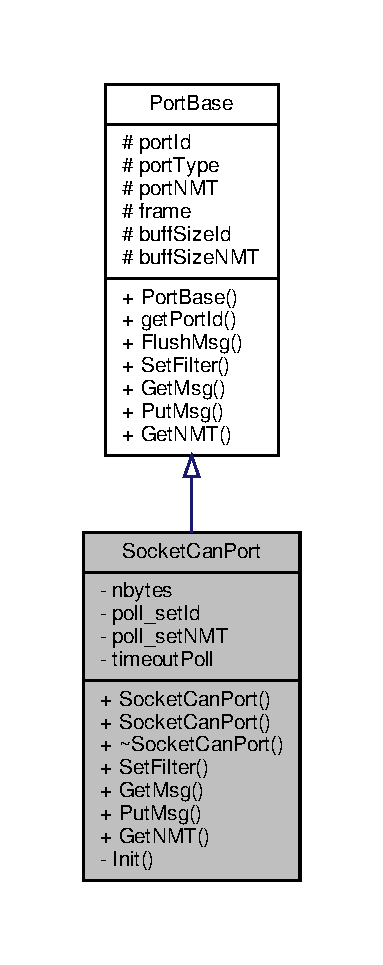
\includegraphics[width=184pt]{classSocketCanPort__inherit__graph}
\end{center}
\end{figure}


Collaboration diagram for Socket\+Can\+Port\+:
\nopagebreak
\begin{figure}[H]
\begin{center}
\leavevmode
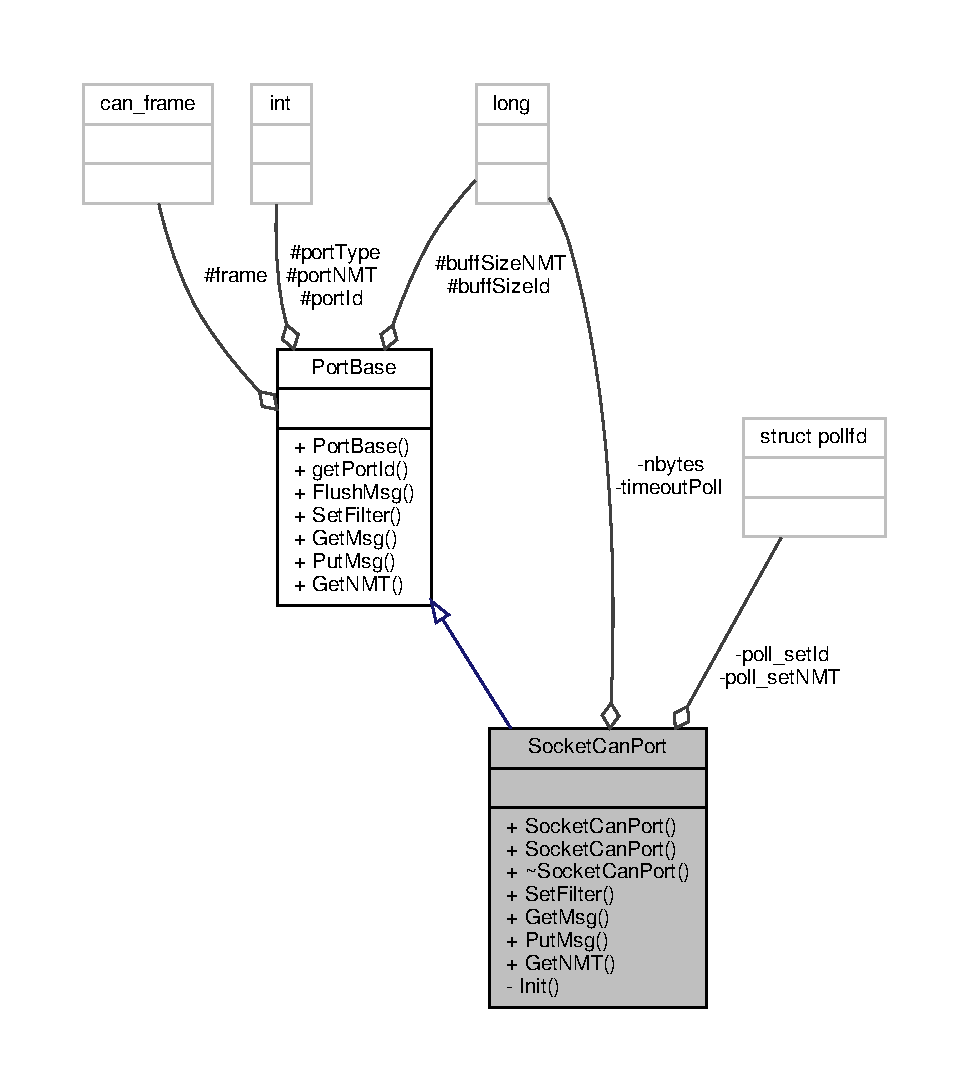
\includegraphics[width=350pt]{classSocketCanPort__coll__graph}
\end{center}
\end{figure}
\subsection*{Public Member Functions}
\begin{DoxyCompactItemize}
\item 
\hyperlink{classSocketCanPort_af3593609acea236b10646732e277837f}{Socket\+Can\+Port} ()
\item 
\hyperlink{classSocketCanPort_a087bc07f3c1658e3cb994d85fcb3da5e}{Socket\+Can\+Port} (string can\+Port)
\item 
\hyperlink{classSocketCanPort_a0d004347e49110daa1ee29e1d1bc85c0}{$\sim$\+Socket\+Can\+Port} ()
\item 
long \hyperlink{classSocketCanPort_a1a5d0866524dae11ddff0d1ac22e0dd5}{Set\+Filter} (uint32\+\_\+t can\+Id, uint32\+\_\+t mask)
\item 
long \hyperlink{classSocketCanPort_aa9684efc602da057cb4928d52395af33}{Get\+Msg} (uint32\+\_\+t \&can\+Id, uint8\+\_\+t $\ast$data, uint8\+\_\+t \&size)
\item 
long \hyperlink{classSocketCanPort_a9375a0c1e33978c83ebd188100898633}{Put\+Msg} (const uint32\+\_\+t \&can\+Id, uint8\+\_\+t $\ast$const data, const uint8\+\_\+t size)
\item 
long \hyperlink{classSocketCanPort_a2efe27bd3bb8c8127c89925e1e21535a}{Get\+N\+MT} (uint8\+\_\+t $\ast$data, uint8\+\_\+t \&size)
\end{DoxyCompactItemize}
\subsection*{Private Member Functions}
\begin{DoxyCompactItemize}
\item 
long \hyperlink{classSocketCanPort_a9209d295c98c12ab85ec61773b775bf4}{Init} (string can\+Port)
\end{DoxyCompactItemize}
\subsection*{Private Attributes}
\begin{DoxyCompactItemize}
\item 
long \hyperlink{classSocketCanPort_a7b06b4d8c897c1a189329f20632fdb71}{nbytes}
\item 
struct pollfd \hyperlink{classSocketCanPort_ad0374fe5ea78a061e7abd16b812f44d5}{poll\+\_\+set\+Id} \mbox{[}1\mbox{]}
\item 
struct pollfd \hyperlink{classSocketCanPort_afaaf9cd49684de93be7370988ec64b47}{poll\+\_\+set\+N\+MT} \mbox{[}1\mbox{]}
\item 
long \hyperlink{classSocketCanPort_a18e670bf7f98482e022da2fd11264309}{timeout\+Poll}
\end{DoxyCompactItemize}
\subsection*{Additional Inherited Members}


\subsection{Constructor \& Destructor Documentation}
\index{Socket\+Can\+Port@{Socket\+Can\+Port}!Socket\+Can\+Port@{Socket\+Can\+Port}}
\index{Socket\+Can\+Port@{Socket\+Can\+Port}!Socket\+Can\+Port@{Socket\+Can\+Port}}
\subsubsection[{\texorpdfstring{Socket\+Can\+Port()}{SocketCanPort()}}]{\setlength{\rightskip}{0pt plus 5cm}Socket\+Can\+Port\+::\+Socket\+Can\+Port (
\begin{DoxyParamCaption}
{}
\end{DoxyParamCaption}
)}\hypertarget{classSocketCanPort_af3593609acea236b10646732e277837f}{}\label{classSocketCanPort_af3593609acea236b10646732e277837f}
\index{Socket\+Can\+Port@{Socket\+Can\+Port}!Socket\+Can\+Port@{Socket\+Can\+Port}}
\index{Socket\+Can\+Port@{Socket\+Can\+Port}!Socket\+Can\+Port@{Socket\+Can\+Port}}
\subsubsection[{\texorpdfstring{Socket\+Can\+Port(string can\+Port)}{SocketCanPort(string canPort)}}]{\setlength{\rightskip}{0pt plus 5cm}Socket\+Can\+Port\+::\+Socket\+Can\+Port (
\begin{DoxyParamCaption}
\item[{string}]{can\+Port}
\end{DoxyParamCaption}
)}\hypertarget{classSocketCanPort_a087bc07f3c1658e3cb994d85fcb3da5e}{}\label{classSocketCanPort_a087bc07f3c1658e3cb994d85fcb3da5e}
\index{Socket\+Can\+Port@{Socket\+Can\+Port}!````~Socket\+Can\+Port@{$\sim$\+Socket\+Can\+Port}}
\index{````~Socket\+Can\+Port@{$\sim$\+Socket\+Can\+Port}!Socket\+Can\+Port@{Socket\+Can\+Port}}
\subsubsection[{\texorpdfstring{$\sim$\+Socket\+Can\+Port()}{~SocketCanPort()}}]{\setlength{\rightskip}{0pt plus 5cm}Socket\+Can\+Port\+::$\sim$\+Socket\+Can\+Port (
\begin{DoxyParamCaption}
{}
\end{DoxyParamCaption}
)}\hypertarget{classSocketCanPort_a0d004347e49110daa1ee29e1d1bc85c0}{}\label{classSocketCanPort_a0d004347e49110daa1ee29e1d1bc85c0}


\subsection{Member Function Documentation}
\index{Socket\+Can\+Port@{Socket\+Can\+Port}!Get\+Msg@{Get\+Msg}}
\index{Get\+Msg@{Get\+Msg}!Socket\+Can\+Port@{Socket\+Can\+Port}}
\subsubsection[{\texorpdfstring{Get\+Msg(uint32\+\_\+t \&can\+Id, uint8\+\_\+t $\ast$data, uint8\+\_\+t \&size)}{GetMsg(uint32_t &canId, uint8_t *data, uint8_t &size)}}]{\setlength{\rightskip}{0pt plus 5cm}long Socket\+Can\+Port\+::\+Get\+Msg (
\begin{DoxyParamCaption}
\item[{uint32\+\_\+t \&}]{can\+Id, }
\item[{uint8\+\_\+t $\ast$}]{data, }
\item[{uint8\+\_\+t \&}]{size}
\end{DoxyParamCaption}
)\hspace{0.3cm}{\ttfamily [virtual]}}\hypertarget{classSocketCanPort_aa9684efc602da057cb4928d52395af33}{}\label{classSocketCanPort_aa9684efc602da057cb4928d52395af33}


Implements \hyperlink{classPortBase_a4fe82768f2b79889d7084292ac0e8696}{Port\+Base}.

\index{Socket\+Can\+Port@{Socket\+Can\+Port}!Get\+N\+MT@{Get\+N\+MT}}
\index{Get\+N\+MT@{Get\+N\+MT}!Socket\+Can\+Port@{Socket\+Can\+Port}}
\subsubsection[{\texorpdfstring{Get\+N\+M\+T(uint8\+\_\+t $\ast$data, uint8\+\_\+t \&size)}{GetNMT(uint8_t *data, uint8_t &size)}}]{\setlength{\rightskip}{0pt plus 5cm}long Socket\+Can\+Port\+::\+Get\+N\+MT (
\begin{DoxyParamCaption}
\item[{uint8\+\_\+t $\ast$}]{data, }
\item[{uint8\+\_\+t \&}]{size}
\end{DoxyParamCaption}
)\hspace{0.3cm}{\ttfamily [virtual]}}\hypertarget{classSocketCanPort_a2efe27bd3bb8c8127c89925e1e21535a}{}\label{classSocketCanPort_a2efe27bd3bb8c8127c89925e1e21535a}


Implements \hyperlink{classPortBase_abab2bf17b01d87c2bca01cb2151aa2f1}{Port\+Base}.

\index{Socket\+Can\+Port@{Socket\+Can\+Port}!Init@{Init}}
\index{Init@{Init}!Socket\+Can\+Port@{Socket\+Can\+Port}}
\subsubsection[{\texorpdfstring{Init(string can\+Port)}{Init(string canPort)}}]{\setlength{\rightskip}{0pt plus 5cm}long Socket\+Can\+Port\+::\+Init (
\begin{DoxyParamCaption}
\item[{string}]{can\+Port}
\end{DoxyParamCaption}
)\hspace{0.3cm}{\ttfamily [private]}}\hypertarget{classSocketCanPort_a9209d295c98c12ab85ec61773b775bf4}{}\label{classSocketCanPort_a9209d295c98c12ab85ec61773b775bf4}
\index{Socket\+Can\+Port@{Socket\+Can\+Port}!Put\+Msg@{Put\+Msg}}
\index{Put\+Msg@{Put\+Msg}!Socket\+Can\+Port@{Socket\+Can\+Port}}
\subsubsection[{\texorpdfstring{Put\+Msg(const uint32\+\_\+t \&can\+Id, uint8\+\_\+t $\ast$const data, const uint8\+\_\+t size)}{PutMsg(const uint32_t &canId, uint8_t *const data, const uint8_t size)}}]{\setlength{\rightskip}{0pt plus 5cm}long Socket\+Can\+Port\+::\+Put\+Msg (
\begin{DoxyParamCaption}
\item[{const uint32\+\_\+t \&}]{can\+Id, }
\item[{uint8\+\_\+t $\ast$const}]{data, }
\item[{const uint8\+\_\+t}]{size}
\end{DoxyParamCaption}
)\hspace{0.3cm}{\ttfamily [virtual]}}\hypertarget{classSocketCanPort_a9375a0c1e33978c83ebd188100898633}{}\label{classSocketCanPort_a9375a0c1e33978c83ebd188100898633}


Implements \hyperlink{classPortBase_a26213ebb6ea0a0b77f60c28944e3bb8e}{Port\+Base}.

\index{Socket\+Can\+Port@{Socket\+Can\+Port}!Set\+Filter@{Set\+Filter}}
\index{Set\+Filter@{Set\+Filter}!Socket\+Can\+Port@{Socket\+Can\+Port}}
\subsubsection[{\texorpdfstring{Set\+Filter(uint32\+\_\+t can\+Id, uint32\+\_\+t mask)}{SetFilter(uint32_t canId, uint32_t mask)}}]{\setlength{\rightskip}{0pt plus 5cm}long Socket\+Can\+Port\+::\+Set\+Filter (
\begin{DoxyParamCaption}
\item[{uint32\+\_\+t}]{can\+Id, }
\item[{uint32\+\_\+t}]{mask}
\end{DoxyParamCaption}
)\hspace{0.3cm}{\ttfamily [virtual]}}\hypertarget{classSocketCanPort_a1a5d0866524dae11ddff0d1ac22e0dd5}{}\label{classSocketCanPort_a1a5d0866524dae11ddff0d1ac22e0dd5}


Implements \hyperlink{classPortBase_a1d857a81a8e3f3bd460ef7c802ee762c}{Port\+Base}.



\subsection{Member Data Documentation}
\index{Socket\+Can\+Port@{Socket\+Can\+Port}!nbytes@{nbytes}}
\index{nbytes@{nbytes}!Socket\+Can\+Port@{Socket\+Can\+Port}}
\subsubsection[{\texorpdfstring{nbytes}{nbytes}}]{\setlength{\rightskip}{0pt plus 5cm}long Socket\+Can\+Port\+::nbytes\hspace{0.3cm}{\ttfamily [private]}}\hypertarget{classSocketCanPort_a7b06b4d8c897c1a189329f20632fdb71}{}\label{classSocketCanPort_a7b06b4d8c897c1a189329f20632fdb71}
\index{Socket\+Can\+Port@{Socket\+Can\+Port}!poll\+\_\+set\+Id@{poll\+\_\+set\+Id}}
\index{poll\+\_\+set\+Id@{poll\+\_\+set\+Id}!Socket\+Can\+Port@{Socket\+Can\+Port}}
\subsubsection[{\texorpdfstring{poll\+\_\+set\+Id}{poll_setId}}]{\setlength{\rightskip}{0pt plus 5cm}struct pollfd Socket\+Can\+Port\+::poll\+\_\+set\+Id\mbox{[}1\mbox{]}\hspace{0.3cm}{\ttfamily [private]}}\hypertarget{classSocketCanPort_ad0374fe5ea78a061e7abd16b812f44d5}{}\label{classSocketCanPort_ad0374fe5ea78a061e7abd16b812f44d5}
\index{Socket\+Can\+Port@{Socket\+Can\+Port}!poll\+\_\+set\+N\+MT@{poll\+\_\+set\+N\+MT}}
\index{poll\+\_\+set\+N\+MT@{poll\+\_\+set\+N\+MT}!Socket\+Can\+Port@{Socket\+Can\+Port}}
\subsubsection[{\texorpdfstring{poll\+\_\+set\+N\+MT}{poll_setNMT}}]{\setlength{\rightskip}{0pt plus 5cm}struct pollfd Socket\+Can\+Port\+::poll\+\_\+set\+N\+MT\mbox{[}1\mbox{]}\hspace{0.3cm}{\ttfamily [private]}}\hypertarget{classSocketCanPort_afaaf9cd49684de93be7370988ec64b47}{}\label{classSocketCanPort_afaaf9cd49684de93be7370988ec64b47}
\index{Socket\+Can\+Port@{Socket\+Can\+Port}!timeout\+Poll@{timeout\+Poll}}
\index{timeout\+Poll@{timeout\+Poll}!Socket\+Can\+Port@{Socket\+Can\+Port}}
\subsubsection[{\texorpdfstring{timeout\+Poll}{timeoutPoll}}]{\setlength{\rightskip}{0pt plus 5cm}long Socket\+Can\+Port\+::timeout\+Poll\hspace{0.3cm}{\ttfamily [private]}}\hypertarget{classSocketCanPort_a18e670bf7f98482e022da2fd11264309}{}\label{classSocketCanPort_a18e670bf7f98482e022da2fd11264309}


The documentation for this class was generated from the following files\+:\begin{DoxyCompactItemize}
\item 
\hyperlink{SocketCanPort_8h}{Socket\+Can\+Port.\+h}\item 
\hyperlink{SocketCanPort_8cpp}{Socket\+Can\+Port.\+cpp}\end{DoxyCompactItemize}

\hypertarget{classTestPort}{}\section{Test\+Port Class Reference}
\label{classTestPort}\index{Test\+Port@{Test\+Port}}


{\ttfamily \#include $<$Test\+Port.\+h$>$}



Inheritance diagram for Test\+Port\+:
\nopagebreak
\begin{figure}[H]
\begin{center}
\leavevmode
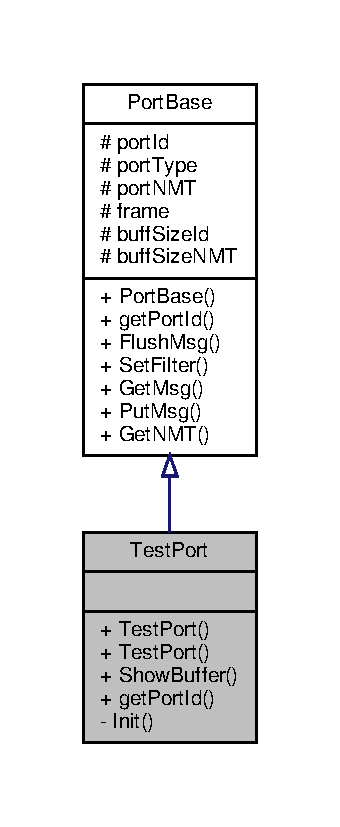
\includegraphics[width=163pt]{classTestPort__inherit__graph}
\end{center}
\end{figure}


Collaboration diagram for Test\+Port\+:
\nopagebreak
\begin{figure}[H]
\begin{center}
\leavevmode
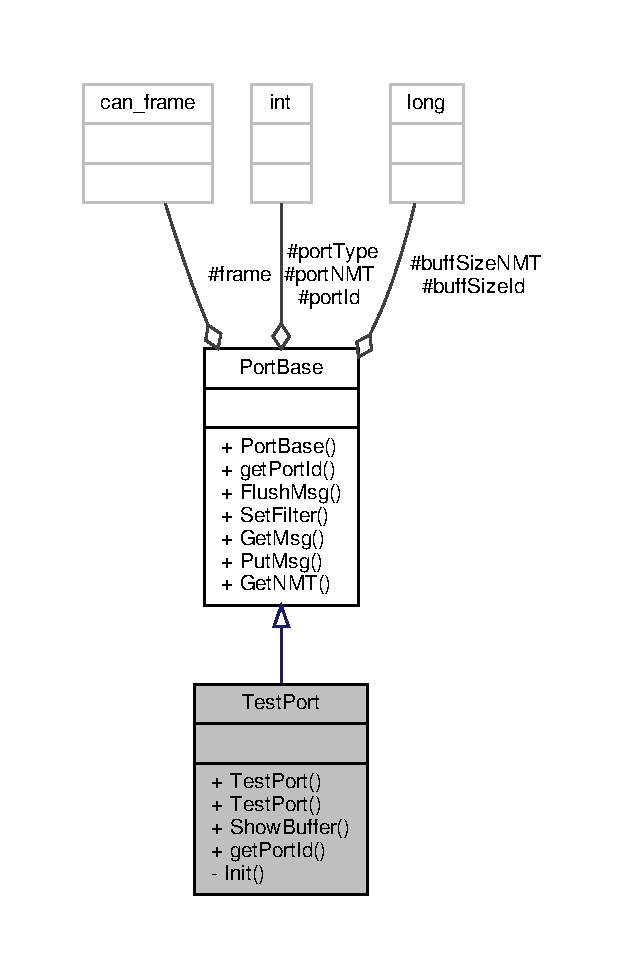
\includegraphics[width=301pt]{classTestPort__coll__graph}
\end{center}
\end{figure}
\subsection*{Public Member Functions}
\begin{DoxyCompactItemize}
\item 
\hyperlink{classTestPort_adde46780527e08b738eb5b32defa1c3a}{Test\+Port} ()
\item 
\hyperlink{classTestPort_a93293d14818c76db0b4ef1273cf5ce19}{Test\+Port} (string Port)
\item 
long \hyperlink{classTestPort_acc9bf1db6c1ca7d9040591306100ab36}{Show\+Buffer} ()
\item 
int \hyperlink{classTestPort_abf6a7327e26838aaf3e2e4482668085f}{get\+Port\+Id} ()
\end{DoxyCompactItemize}
\subsection*{Private Member Functions}
\begin{DoxyCompactItemize}
\item 
long \hyperlink{classTestPort_adbc256fed358ebb6bf3243ccd187170f}{Init} (string name)
\end{DoxyCompactItemize}
\subsection*{Additional Inherited Members}


\subsection{Constructor \& Destructor Documentation}
\index{Test\+Port@{Test\+Port}!Test\+Port@{Test\+Port}}
\index{Test\+Port@{Test\+Port}!Test\+Port@{Test\+Port}}
\subsubsection[{\texorpdfstring{Test\+Port()}{TestPort()}}]{\setlength{\rightskip}{0pt plus 5cm}Test\+Port\+::\+Test\+Port (
\begin{DoxyParamCaption}
{}
\end{DoxyParamCaption}
)}\hypertarget{classTestPort_adde46780527e08b738eb5b32defa1c3a}{}\label{classTestPort_adde46780527e08b738eb5b32defa1c3a}
\index{Test\+Port@{Test\+Port}!Test\+Port@{Test\+Port}}
\index{Test\+Port@{Test\+Port}!Test\+Port@{Test\+Port}}
\subsubsection[{\texorpdfstring{Test\+Port(string Port)}{TestPort(string Port)}}]{\setlength{\rightskip}{0pt plus 5cm}Test\+Port\+::\+Test\+Port (
\begin{DoxyParamCaption}
\item[{string}]{Port}
\end{DoxyParamCaption}
)}\hypertarget{classTestPort_a93293d14818c76db0b4ef1273cf5ce19}{}\label{classTestPort_a93293d14818c76db0b4ef1273cf5ce19}


\subsection{Member Function Documentation}
\index{Test\+Port@{Test\+Port}!get\+Port\+Id@{get\+Port\+Id}}
\index{get\+Port\+Id@{get\+Port\+Id}!Test\+Port@{Test\+Port}}
\subsubsection[{\texorpdfstring{get\+Port\+Id()}{getPortId()}}]{\setlength{\rightskip}{0pt plus 5cm}int Test\+Port\+::get\+Port\+Id (
\begin{DoxyParamCaption}
{}
\end{DoxyParamCaption}
)}\hypertarget{classTestPort_abf6a7327e26838aaf3e2e4482668085f}{}\label{classTestPort_abf6a7327e26838aaf3e2e4482668085f}
\index{Test\+Port@{Test\+Port}!Init@{Init}}
\index{Init@{Init}!Test\+Port@{Test\+Port}}
\subsubsection[{\texorpdfstring{Init(string name)}{Init(string name)}}]{\setlength{\rightskip}{0pt plus 5cm}long Test\+Port\+::\+Init (
\begin{DoxyParamCaption}
\item[{string}]{name}
\end{DoxyParamCaption}
)\hspace{0.3cm}{\ttfamily [private]}}\hypertarget{classTestPort_adbc256fed358ebb6bf3243ccd187170f}{}\label{classTestPort_adbc256fed358ebb6bf3243ccd187170f}
\index{Test\+Port@{Test\+Port}!Show\+Buffer@{Show\+Buffer}}
\index{Show\+Buffer@{Show\+Buffer}!Test\+Port@{Test\+Port}}
\subsubsection[{\texorpdfstring{Show\+Buffer()}{ShowBuffer()}}]{\setlength{\rightskip}{0pt plus 5cm}long Test\+Port\+::\+Show\+Buffer (
\begin{DoxyParamCaption}
{}
\end{DoxyParamCaption}
)}\hypertarget{classTestPort_acc9bf1db6c1ca7d9040591306100ab36}{}\label{classTestPort_acc9bf1db6c1ca7d9040591306100ab36}


The documentation for this class was generated from the following files\+:\begin{DoxyCompactItemize}
\item 
\hyperlink{TestPort_8h}{Test\+Port.\+h}\item 
\hyperlink{TestPort_8cpp}{Test\+Port.\+cpp}\end{DoxyCompactItemize}

\chapter{File Documentation}
\hypertarget{CanBusPort_8cpp}{}\section{Can\+Bus\+Port.\+cpp File Reference}
\label{CanBusPort_8cpp}\index{Can\+Bus\+Port.\+cpp@{Can\+Bus\+Port.\+cpp}}
{\ttfamily \#include \char`\"{}Can\+Bus\+Port.\+h\char`\"{}}\\*
Include dependency graph for Can\+Bus\+Port.\+cpp\+:
\nopagebreak
\begin{figure}[H]
\begin{center}
\leavevmode
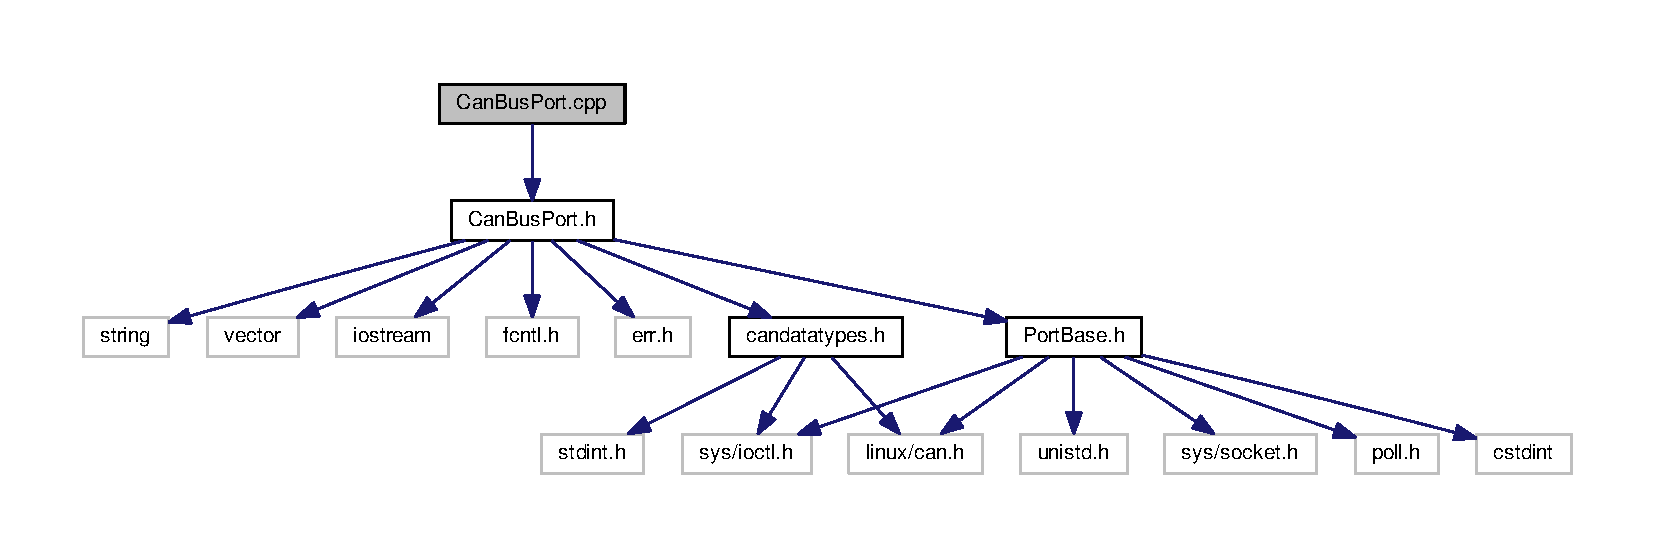
\includegraphics[width=350pt]{CanBusPort_8cpp__incl}
\end{center}
\end{figure}

\hypertarget{CanBusPort_8h}{}\section{Can\+Bus\+Port.\+h File Reference}
\label{CanBusPort_8h}\index{Can\+Bus\+Port.\+h@{Can\+Bus\+Port.\+h}}
{\ttfamily \#include $<$string$>$}\\*
{\ttfamily \#include $<$vector$>$}\\*
{\ttfamily \#include $<$iostream$>$}\\*
{\ttfamily \#include $<$fcntl.\+h$>$}\\*
{\ttfamily \#include $<$err.\+h$>$}\\*
{\ttfamily \#include \char`\"{}candatatypes.\+h\char`\"{}}\\*
{\ttfamily \#include \char`\"{}Port\+Base.\+h\char`\"{}}\\*
Include dependency graph for Can\+Bus\+Port.\+h\+:
\nopagebreak
\begin{figure}[H]
\begin{center}
\leavevmode
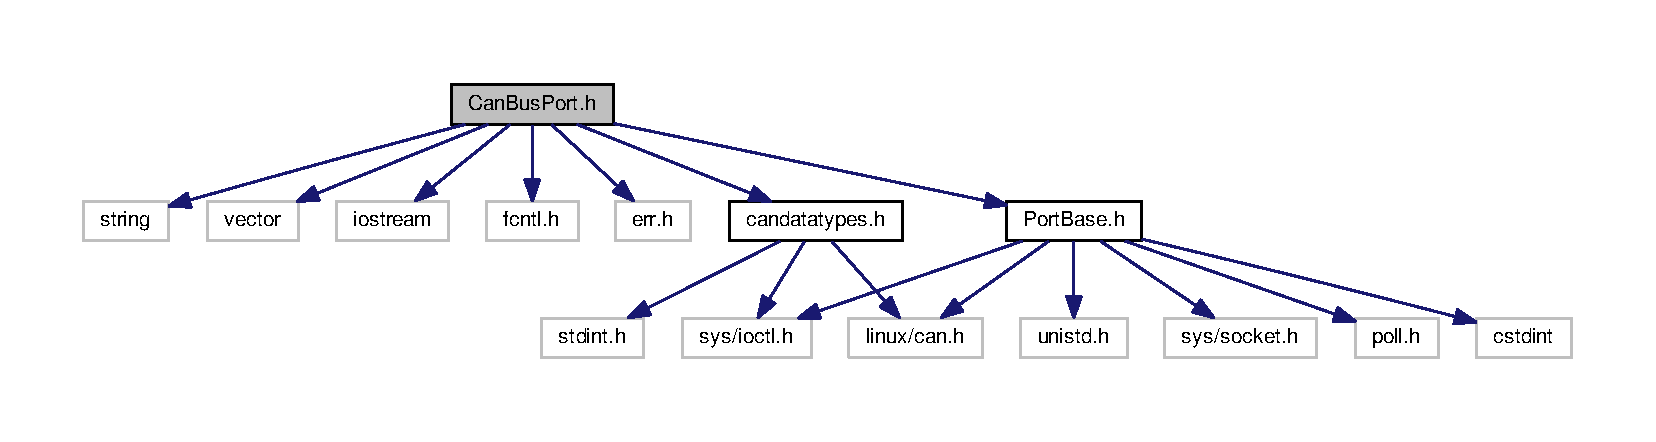
\includegraphics[width=350pt]{CanBusPort_8h__incl}
\end{center}
\end{figure}
This graph shows which files directly or indirectly include this file\+:
\nopagebreak
\begin{figure}[H]
\begin{center}
\leavevmode
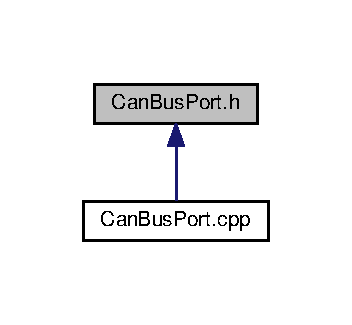
\includegraphics[width=169pt]{CanBusPort_8h__dep__incl}
\end{center}
\end{figure}
\subsection*{Classes}
\begin{DoxyCompactItemize}
\item 
class \hyperlink{classCanBusPort}{Can\+Bus\+Port}
\end{DoxyCompactItemize}

\hypertarget{candatatypes_8h}{}\section{candatatypes.\+h File Reference}
\label{candatatypes_8h}\index{candatatypes.\+h@{candatatypes.\+h}}
{\ttfamily \#include $<$linux/can.\+h$>$}\\*
{\ttfamily \#include $<$sys/ioctl.\+h$>$}\\*
{\ttfamily \#include $<$stdint.\+h$>$}\\*
Include dependency graph for candatatypes.\+h\+:
\nopagebreak
\begin{figure}[H]
\begin{center}
\leavevmode
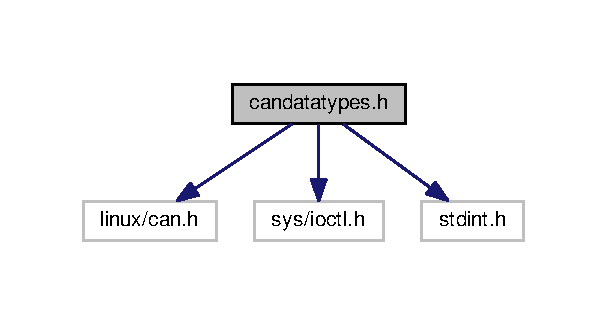
\includegraphics[width=292pt]{candatatypes_8h__incl}
\end{center}
\end{figure}
This graph shows which files directly or indirectly include this file\+:
\nopagebreak
\begin{figure}[H]
\begin{center}
\leavevmode
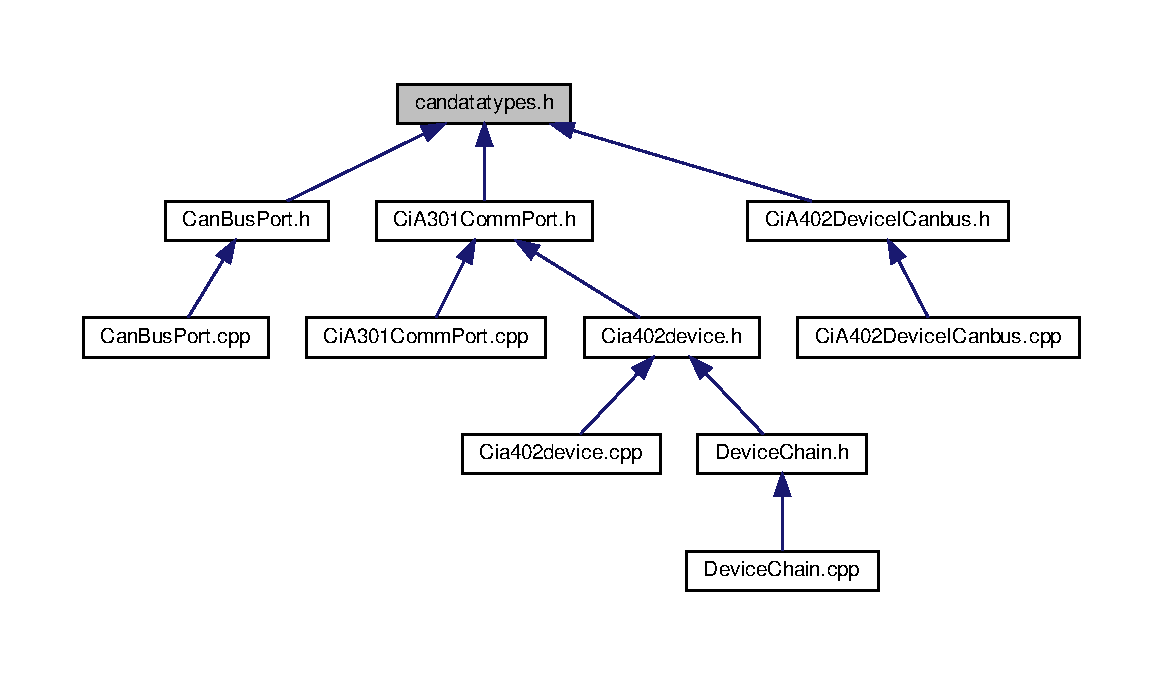
\includegraphics[width=350pt]{candatatypes_8h__dep__incl}
\end{center}
\end{figure}
\subsection*{Classes}
\begin{DoxyCompactItemize}
\item 
struct \hyperlink{structcan__msg}{can\+\_\+msg}
\item 
struct \hyperlink{structco__msg}{co\+\_\+msg}
\end{DoxyCompactItemize}
\subsection*{Macros}
\begin{DoxyCompactItemize}
\item 
\#define \hyperlink{candatatypes_8h_a37499575cbfb9909399ce3189639f122}{G\+E\+T\+\_\+\+N\+O\+D\+E\+\_\+\+ID}(cobid)~( cobid \& 0x7f )
\item 
\#define \hyperlink{candatatypes_8h_abb973a44d16fd02957aec9c47d5ac0b1}{I\+O\+C\+\_\+\+M\+A\+G\+IC}~\textquotesingle{}E\textquotesingle{}
\item 
\#define \hyperlink{candatatypes_8h_a36d525cf4d116b2fe4ecc00222b256f1}{P\+A\+C\+K\+ED}~\+\_\+\+\_\+attribute\+\_\+\+\_\+((packed))
\item 
\#define \hyperlink{candatatypes_8h_a0e6b1af48bd887e8d0c978b5dc7307bc}{M\+S\+G\+\_\+\+D\+LC}(msg)~(((msg)-\/$>$fi\&0xf)$>$$>$0)
\item 
\#define \hyperlink{candatatypes_8h_a3e5172a02bebe6e5e9706ab7df06d902}{M\+S\+G\+\_\+\+R\+TR}(msg)~(((msg)-\/$>$fi\&(1$<$$<$4))$>$$>$4)
\item 
\#define \hyperlink{candatatypes_8h_af5de903edfa22afc007f582fa19cb3d9}{M\+S\+G\+\_\+\+FF}(msg)~(((msg)-\/$>$fi\&(1$<$$<$5))$>$$>$5)
\item 
\#define \hyperlink{candatatypes_8h_a5525b28635b17a750eb630af9f82aabf}{M\+S\+G\+\_\+\+D\+OS}(msg)~(((msg)-\/$>$fi\&(1$<$$<$6))$>$$>$6)
\item 
\#define \hyperlink{candatatypes_8h_a5682e4e8de03fe4232894a36ff00b316}{M\+S\+G\+\_\+\+I\+O\+P\+IN}(msg)~(((msg)-\/$>$fi\&(1$<$$<$7))$>$$>$7)
\item 
\#define \hyperlink{candatatypes_8h_a4ad56e164b5ddbdec986135493a1fef2}{M\+S\+G\+\_\+\+N\+O\+DE}(msg)~(((msg)-\/$>$fi\&(3$<$$<$8))$>$$>$8)
\item 
\#define \hyperlink{candatatypes_8h_a04fd6b5cadb7a6b3d7b586a14545ccdb}{F\+F\+\_\+\+N\+O\+R\+M\+AL}~0
\item 
\#define \hyperlink{candatatypes_8h_a45b12438f26b30925139689e606f9231}{F\+F\+\_\+\+E\+X\+T\+E\+N\+D\+ED}~1
\item 
\#define \hyperlink{candatatypes_8h_a2e1908762e3be59ff1f1249315817f3f}{I\+O\+C\+\_\+\+R\+E\+S\+E\+T\+\_\+\+B\+O\+A\+RD}~\+\_\+\+IO (\hyperlink{hico__api_8h_abb973a44d16fd02957aec9c47d5ac0b1}{I\+O\+C\+\_\+\+M\+A\+G\+IC}, 1)
\item 
\#define \hyperlink{candatatypes_8h_a346da60de0bcf2ba4fe6d83c2439a6aa}{I\+O\+C\+\_\+\+S\+T\+A\+RT}~\+\_\+\+IO (\hyperlink{hico__api_8h_abb973a44d16fd02957aec9c47d5ac0b1}{I\+O\+C\+\_\+\+M\+A\+G\+IC}, 5)
\item 
\#define \hyperlink{candatatypes_8h_a23b340dcb801bd677be094b1db214f21}{I\+O\+C\+\_\+\+S\+T\+A\+R\+T\+\_\+\+P\+A\+S\+S\+I\+VE}~\+\_\+\+IO (\hyperlink{hico__api_8h_abb973a44d16fd02957aec9c47d5ac0b1}{I\+O\+C\+\_\+\+M\+A\+G\+IC}, 10)
\item 
\#define \hyperlink{candatatypes_8h_af8cda96f7edddada586e67abc795c9a7}{I\+O\+C\+\_\+\+S\+T\+A\+R\+T\+\_\+\+B\+A\+U\+D\+S\+C\+AN}~\+\_\+\+IO (\hyperlink{hico__api_8h_abb973a44d16fd02957aec9c47d5ac0b1}{I\+O\+C\+\_\+\+M\+A\+G\+IC}, 15)
\item 
\#define \hyperlink{candatatypes_8h_a25a17d51ed18d29864905396e2542f2a}{I\+O\+C\+\_\+\+S\+T\+OP}~\+\_\+\+IO (\hyperlink{hico__api_8h_abb973a44d16fd02957aec9c47d5ac0b1}{I\+O\+C\+\_\+\+M\+A\+G\+IC}, 20)
\item 
\#define \hyperlink{candatatypes_8h_a435f17e5332c2081e7ce09842664f183}{I\+O\+C\+\_\+\+G\+E\+T\+\_\+\+M\+O\+DE}~\+\_\+\+I\+OR(\hyperlink{hico__api_8h_abb973a44d16fd02957aec9c47d5ac0b1}{I\+O\+C\+\_\+\+M\+A\+G\+IC}, 25,  uint32\+\_\+t)
\item 
\#define \hyperlink{candatatypes_8h_aff568c17dcaa5179a247a36874b011f6}{C\+M\+\_\+\+B\+A\+U\+D\+S\+C\+AN}~1
\item 
\#define \hyperlink{candatatypes_8h_ac16bf18f66fbaf440f3dedf069a0f611}{C\+M\+\_\+\+P\+A\+S\+S\+I\+VE}~2
\item 
\#define \hyperlink{candatatypes_8h_a6c1e851b693474b1b91bb0820adfbce3}{C\+M\+\_\+\+A\+C\+T\+I\+VE}~3
\item 
\#define \hyperlink{candatatypes_8h_aa8bcd6538691e59322e8e3a03fad080a}{C\+M\+\_\+\+R\+E\+S\+ET}~4
\item 
\#define \hyperlink{candatatypes_8h_a9bcc4d1b52c43e507f264eb3d326f1c5}{I\+O\+C\+\_\+\+S\+E\+T\+\_\+\+B\+I\+T\+R\+A\+TE}~\+\_\+\+I\+OW (\hyperlink{hico__api_8h_abb973a44d16fd02957aec9c47d5ac0b1}{I\+O\+C\+\_\+\+M\+A\+G\+IC}, 30, uint32\+\_\+t)
\item 
\#define \hyperlink{candatatypes_8h_aa1ad7a89155a7f858ab52149c2fcaad5}{B\+I\+T\+R\+A\+T\+E\+\_\+10k}~0
\item 
\#define \hyperlink{candatatypes_8h_a4eb46432ed1b9dd664fc642738a1a969}{B\+I\+T\+R\+A\+T\+E\+\_\+20k}~1
\item 
\#define \hyperlink{candatatypes_8h_a39c91c0deb48d0a15d084f2a2021417b}{B\+I\+T\+R\+A\+T\+E\+\_\+50k}~2
\item 
\#define \hyperlink{candatatypes_8h_aae6f862ae12a0da0d319cd353ea7befe}{B\+I\+T\+R\+A\+T\+E\+\_\+100k}~3
\item 
\#define \hyperlink{candatatypes_8h_afbce0ed8bc362c29562f98ea81456e24}{B\+I\+T\+R\+A\+T\+E\+\_\+125k}~4
\item 
\#define \hyperlink{candatatypes_8h_a634a59a9129b549f182844e7b4058a2a}{B\+I\+T\+R\+A\+T\+E\+\_\+250k}~5
\item 
\#define \hyperlink{candatatypes_8h_a845bd49223fdabd4ebd206779eb8f3b1}{B\+I\+T\+R\+A\+T\+E\+\_\+500k}~6
\item 
\#define \hyperlink{candatatypes_8h_a8b1930fb9b23dcba55143e0ef37081fc}{B\+I\+T\+R\+A\+T\+E\+\_\+800k}~7
\item 
\#define \hyperlink{candatatypes_8h_a1432cd8532548faf2ae5287ca4a7413c}{B\+I\+T\+R\+A\+T\+E\+\_\+1000k}~8
\item 
\#define \hyperlink{candatatypes_8h_a9b5344964c96f46fcfffc44074a499a5}{I\+O\+C\+\_\+\+S\+E\+T\+\_\+\+S\+J\+W\+\_\+\+I\+N\+C\+R\+E\+M\+E\+NT}~\+\_\+\+I\+OW (\hyperlink{hico__api_8h_abb973a44d16fd02957aec9c47d5ac0b1}{I\+O\+C\+\_\+\+M\+A\+G\+IC}, 31, uint32\+\_\+t)
\item 
\#define \hyperlink{candatatypes_8h_a1be0497522ab2fd1aa5b9f7eaecda4fb}{I\+O\+C\+\_\+\+G\+E\+T\+\_\+\+B\+I\+T\+R\+A\+TE}~\+\_\+\+I\+OR (\hyperlink{hico__api_8h_abb973a44d16fd02957aec9c47d5ac0b1}{I\+O\+C\+\_\+\+M\+A\+G\+IC}, 35, uint32\+\_\+t)
\end{DoxyCompactItemize}
\subsection*{Variables}
\begin{DoxyCompactItemize}
\item 
struct \hyperlink{structcan__msg}{can\+\_\+msg} \hyperlink{candatatypes_8h_aaf243a2c10c3bb6ce08d79a9637a9a47}{P\+A\+C\+K\+ED}
\end{DoxyCompactItemize}


\subsection{Macro Definition Documentation}
\index{candatatypes.\+h@{candatatypes.\+h}!B\+I\+T\+R\+A\+T\+E\+\_\+1000k@{B\+I\+T\+R\+A\+T\+E\+\_\+1000k}}
\index{B\+I\+T\+R\+A\+T\+E\+\_\+1000k@{B\+I\+T\+R\+A\+T\+E\+\_\+1000k}!candatatypes.\+h@{candatatypes.\+h}}
\subsubsection[{\texorpdfstring{B\+I\+T\+R\+A\+T\+E\+\_\+1000k}{BITRATE_1000k}}]{\setlength{\rightskip}{0pt plus 5cm}\#define B\+I\+T\+R\+A\+T\+E\+\_\+1000k~8}\hypertarget{candatatypes_8h_a1432cd8532548faf2ae5287ca4a7413c}{}\label{candatatypes_8h_a1432cd8532548faf2ae5287ca4a7413c}
\index{candatatypes.\+h@{candatatypes.\+h}!B\+I\+T\+R\+A\+T\+E\+\_\+100k@{B\+I\+T\+R\+A\+T\+E\+\_\+100k}}
\index{B\+I\+T\+R\+A\+T\+E\+\_\+100k@{B\+I\+T\+R\+A\+T\+E\+\_\+100k}!candatatypes.\+h@{candatatypes.\+h}}
\subsubsection[{\texorpdfstring{B\+I\+T\+R\+A\+T\+E\+\_\+100k}{BITRATE_100k}}]{\setlength{\rightskip}{0pt plus 5cm}\#define B\+I\+T\+R\+A\+T\+E\+\_\+100k~3}\hypertarget{candatatypes_8h_aae6f862ae12a0da0d319cd353ea7befe}{}\label{candatatypes_8h_aae6f862ae12a0da0d319cd353ea7befe}
\index{candatatypes.\+h@{candatatypes.\+h}!B\+I\+T\+R\+A\+T\+E\+\_\+10k@{B\+I\+T\+R\+A\+T\+E\+\_\+10k}}
\index{B\+I\+T\+R\+A\+T\+E\+\_\+10k@{B\+I\+T\+R\+A\+T\+E\+\_\+10k}!candatatypes.\+h@{candatatypes.\+h}}
\subsubsection[{\texorpdfstring{B\+I\+T\+R\+A\+T\+E\+\_\+10k}{BITRATE_10k}}]{\setlength{\rightskip}{0pt plus 5cm}\#define B\+I\+T\+R\+A\+T\+E\+\_\+10k~0}\hypertarget{candatatypes_8h_aa1ad7a89155a7f858ab52149c2fcaad5}{}\label{candatatypes_8h_aa1ad7a89155a7f858ab52149c2fcaad5}
\index{candatatypes.\+h@{candatatypes.\+h}!B\+I\+T\+R\+A\+T\+E\+\_\+125k@{B\+I\+T\+R\+A\+T\+E\+\_\+125k}}
\index{B\+I\+T\+R\+A\+T\+E\+\_\+125k@{B\+I\+T\+R\+A\+T\+E\+\_\+125k}!candatatypes.\+h@{candatatypes.\+h}}
\subsubsection[{\texorpdfstring{B\+I\+T\+R\+A\+T\+E\+\_\+125k}{BITRATE_125k}}]{\setlength{\rightskip}{0pt plus 5cm}\#define B\+I\+T\+R\+A\+T\+E\+\_\+125k~4}\hypertarget{candatatypes_8h_afbce0ed8bc362c29562f98ea81456e24}{}\label{candatatypes_8h_afbce0ed8bc362c29562f98ea81456e24}
\index{candatatypes.\+h@{candatatypes.\+h}!B\+I\+T\+R\+A\+T\+E\+\_\+20k@{B\+I\+T\+R\+A\+T\+E\+\_\+20k}}
\index{B\+I\+T\+R\+A\+T\+E\+\_\+20k@{B\+I\+T\+R\+A\+T\+E\+\_\+20k}!candatatypes.\+h@{candatatypes.\+h}}
\subsubsection[{\texorpdfstring{B\+I\+T\+R\+A\+T\+E\+\_\+20k}{BITRATE_20k}}]{\setlength{\rightskip}{0pt plus 5cm}\#define B\+I\+T\+R\+A\+T\+E\+\_\+20k~1}\hypertarget{candatatypes_8h_a4eb46432ed1b9dd664fc642738a1a969}{}\label{candatatypes_8h_a4eb46432ed1b9dd664fc642738a1a969}
\index{candatatypes.\+h@{candatatypes.\+h}!B\+I\+T\+R\+A\+T\+E\+\_\+250k@{B\+I\+T\+R\+A\+T\+E\+\_\+250k}}
\index{B\+I\+T\+R\+A\+T\+E\+\_\+250k@{B\+I\+T\+R\+A\+T\+E\+\_\+250k}!candatatypes.\+h@{candatatypes.\+h}}
\subsubsection[{\texorpdfstring{B\+I\+T\+R\+A\+T\+E\+\_\+250k}{BITRATE_250k}}]{\setlength{\rightskip}{0pt plus 5cm}\#define B\+I\+T\+R\+A\+T\+E\+\_\+250k~5}\hypertarget{candatatypes_8h_a634a59a9129b549f182844e7b4058a2a}{}\label{candatatypes_8h_a634a59a9129b549f182844e7b4058a2a}
\index{candatatypes.\+h@{candatatypes.\+h}!B\+I\+T\+R\+A\+T\+E\+\_\+500k@{B\+I\+T\+R\+A\+T\+E\+\_\+500k}}
\index{B\+I\+T\+R\+A\+T\+E\+\_\+500k@{B\+I\+T\+R\+A\+T\+E\+\_\+500k}!candatatypes.\+h@{candatatypes.\+h}}
\subsubsection[{\texorpdfstring{B\+I\+T\+R\+A\+T\+E\+\_\+500k}{BITRATE_500k}}]{\setlength{\rightskip}{0pt plus 5cm}\#define B\+I\+T\+R\+A\+T\+E\+\_\+500k~6}\hypertarget{candatatypes_8h_a845bd49223fdabd4ebd206779eb8f3b1}{}\label{candatatypes_8h_a845bd49223fdabd4ebd206779eb8f3b1}
\index{candatatypes.\+h@{candatatypes.\+h}!B\+I\+T\+R\+A\+T\+E\+\_\+50k@{B\+I\+T\+R\+A\+T\+E\+\_\+50k}}
\index{B\+I\+T\+R\+A\+T\+E\+\_\+50k@{B\+I\+T\+R\+A\+T\+E\+\_\+50k}!candatatypes.\+h@{candatatypes.\+h}}
\subsubsection[{\texorpdfstring{B\+I\+T\+R\+A\+T\+E\+\_\+50k}{BITRATE_50k}}]{\setlength{\rightskip}{0pt plus 5cm}\#define B\+I\+T\+R\+A\+T\+E\+\_\+50k~2}\hypertarget{candatatypes_8h_a39c91c0deb48d0a15d084f2a2021417b}{}\label{candatatypes_8h_a39c91c0deb48d0a15d084f2a2021417b}
\index{candatatypes.\+h@{candatatypes.\+h}!B\+I\+T\+R\+A\+T\+E\+\_\+800k@{B\+I\+T\+R\+A\+T\+E\+\_\+800k}}
\index{B\+I\+T\+R\+A\+T\+E\+\_\+800k@{B\+I\+T\+R\+A\+T\+E\+\_\+800k}!candatatypes.\+h@{candatatypes.\+h}}
\subsubsection[{\texorpdfstring{B\+I\+T\+R\+A\+T\+E\+\_\+800k}{BITRATE_800k}}]{\setlength{\rightskip}{0pt plus 5cm}\#define B\+I\+T\+R\+A\+T\+E\+\_\+800k~7}\hypertarget{candatatypes_8h_a8b1930fb9b23dcba55143e0ef37081fc}{}\label{candatatypes_8h_a8b1930fb9b23dcba55143e0ef37081fc}
\index{candatatypes.\+h@{candatatypes.\+h}!C\+M\+\_\+\+A\+C\+T\+I\+VE@{C\+M\+\_\+\+A\+C\+T\+I\+VE}}
\index{C\+M\+\_\+\+A\+C\+T\+I\+VE@{C\+M\+\_\+\+A\+C\+T\+I\+VE}!candatatypes.\+h@{candatatypes.\+h}}
\subsubsection[{\texorpdfstring{C\+M\+\_\+\+A\+C\+T\+I\+VE}{CM_ACTIVE}}]{\setlength{\rightskip}{0pt plus 5cm}\#define C\+M\+\_\+\+A\+C\+T\+I\+VE~3}\hypertarget{candatatypes_8h_a6c1e851b693474b1b91bb0820adfbce3}{}\label{candatatypes_8h_a6c1e851b693474b1b91bb0820adfbce3}
\index{candatatypes.\+h@{candatatypes.\+h}!C\+M\+\_\+\+B\+A\+U\+D\+S\+C\+AN@{C\+M\+\_\+\+B\+A\+U\+D\+S\+C\+AN}}
\index{C\+M\+\_\+\+B\+A\+U\+D\+S\+C\+AN@{C\+M\+\_\+\+B\+A\+U\+D\+S\+C\+AN}!candatatypes.\+h@{candatatypes.\+h}}
\subsubsection[{\texorpdfstring{C\+M\+\_\+\+B\+A\+U\+D\+S\+C\+AN}{CM_BAUDSCAN}}]{\setlength{\rightskip}{0pt plus 5cm}\#define C\+M\+\_\+\+B\+A\+U\+D\+S\+C\+AN~1}\hypertarget{candatatypes_8h_aff568c17dcaa5179a247a36874b011f6}{}\label{candatatypes_8h_aff568c17dcaa5179a247a36874b011f6}
\index{candatatypes.\+h@{candatatypes.\+h}!C\+M\+\_\+\+P\+A\+S\+S\+I\+VE@{C\+M\+\_\+\+P\+A\+S\+S\+I\+VE}}
\index{C\+M\+\_\+\+P\+A\+S\+S\+I\+VE@{C\+M\+\_\+\+P\+A\+S\+S\+I\+VE}!candatatypes.\+h@{candatatypes.\+h}}
\subsubsection[{\texorpdfstring{C\+M\+\_\+\+P\+A\+S\+S\+I\+VE}{CM_PASSIVE}}]{\setlength{\rightskip}{0pt plus 5cm}\#define C\+M\+\_\+\+P\+A\+S\+S\+I\+VE~2}\hypertarget{candatatypes_8h_ac16bf18f66fbaf440f3dedf069a0f611}{}\label{candatatypes_8h_ac16bf18f66fbaf440f3dedf069a0f611}
\index{candatatypes.\+h@{candatatypes.\+h}!C\+M\+\_\+\+R\+E\+S\+ET@{C\+M\+\_\+\+R\+E\+S\+ET}}
\index{C\+M\+\_\+\+R\+E\+S\+ET@{C\+M\+\_\+\+R\+E\+S\+ET}!candatatypes.\+h@{candatatypes.\+h}}
\subsubsection[{\texorpdfstring{C\+M\+\_\+\+R\+E\+S\+ET}{CM_RESET}}]{\setlength{\rightskip}{0pt plus 5cm}\#define C\+M\+\_\+\+R\+E\+S\+ET~4}\hypertarget{candatatypes_8h_aa8bcd6538691e59322e8e3a03fad080a}{}\label{candatatypes_8h_aa8bcd6538691e59322e8e3a03fad080a}
\index{candatatypes.\+h@{candatatypes.\+h}!F\+F\+\_\+\+E\+X\+T\+E\+N\+D\+ED@{F\+F\+\_\+\+E\+X\+T\+E\+N\+D\+ED}}
\index{F\+F\+\_\+\+E\+X\+T\+E\+N\+D\+ED@{F\+F\+\_\+\+E\+X\+T\+E\+N\+D\+ED}!candatatypes.\+h@{candatatypes.\+h}}
\subsubsection[{\texorpdfstring{F\+F\+\_\+\+E\+X\+T\+E\+N\+D\+ED}{FF_EXTENDED}}]{\setlength{\rightskip}{0pt plus 5cm}\#define F\+F\+\_\+\+E\+X\+T\+E\+N\+D\+ED~1}\hypertarget{candatatypes_8h_a45b12438f26b30925139689e606f9231}{}\label{candatatypes_8h_a45b12438f26b30925139689e606f9231}
\index{candatatypes.\+h@{candatatypes.\+h}!F\+F\+\_\+\+N\+O\+R\+M\+AL@{F\+F\+\_\+\+N\+O\+R\+M\+AL}}
\index{F\+F\+\_\+\+N\+O\+R\+M\+AL@{F\+F\+\_\+\+N\+O\+R\+M\+AL}!candatatypes.\+h@{candatatypes.\+h}}
\subsubsection[{\texorpdfstring{F\+F\+\_\+\+N\+O\+R\+M\+AL}{FF_NORMAL}}]{\setlength{\rightskip}{0pt plus 5cm}\#define F\+F\+\_\+\+N\+O\+R\+M\+AL~0}\hypertarget{candatatypes_8h_a04fd6b5cadb7a6b3d7b586a14545ccdb}{}\label{candatatypes_8h_a04fd6b5cadb7a6b3d7b586a14545ccdb}
\index{candatatypes.\+h@{candatatypes.\+h}!G\+E\+T\+\_\+\+N\+O\+D\+E\+\_\+\+ID@{G\+E\+T\+\_\+\+N\+O\+D\+E\+\_\+\+ID}}
\index{G\+E\+T\+\_\+\+N\+O\+D\+E\+\_\+\+ID@{G\+E\+T\+\_\+\+N\+O\+D\+E\+\_\+\+ID}!candatatypes.\+h@{candatatypes.\+h}}
\subsubsection[{\texorpdfstring{G\+E\+T\+\_\+\+N\+O\+D\+E\+\_\+\+ID}{GET_NODE_ID}}]{\setlength{\rightskip}{0pt plus 5cm}\#define G\+E\+T\+\_\+\+N\+O\+D\+E\+\_\+\+ID(
\begin{DoxyParamCaption}
\item[{}]{cobid}
\end{DoxyParamCaption}
)~( cobid \& 0x7f )}\hypertarget{candatatypes_8h_a37499575cbfb9909399ce3189639f122}{}\label{candatatypes_8h_a37499575cbfb9909399ce3189639f122}
\index{candatatypes.\+h@{candatatypes.\+h}!I\+O\+C\+\_\+\+G\+E\+T\+\_\+\+B\+I\+T\+R\+A\+TE@{I\+O\+C\+\_\+\+G\+E\+T\+\_\+\+B\+I\+T\+R\+A\+TE}}
\index{I\+O\+C\+\_\+\+G\+E\+T\+\_\+\+B\+I\+T\+R\+A\+TE@{I\+O\+C\+\_\+\+G\+E\+T\+\_\+\+B\+I\+T\+R\+A\+TE}!candatatypes.\+h@{candatatypes.\+h}}
\subsubsection[{\texorpdfstring{I\+O\+C\+\_\+\+G\+E\+T\+\_\+\+B\+I\+T\+R\+A\+TE}{IOC_GET_BITRATE}}]{\setlength{\rightskip}{0pt plus 5cm}\#define I\+O\+C\+\_\+\+G\+E\+T\+\_\+\+B\+I\+T\+R\+A\+TE~\+\_\+\+I\+OR ({\bf I\+O\+C\+\_\+\+M\+A\+G\+IC}, 35, uint32\+\_\+t)}\hypertarget{candatatypes_8h_a1be0497522ab2fd1aa5b9f7eaecda4fb}{}\label{candatatypes_8h_a1be0497522ab2fd1aa5b9f7eaecda4fb}
\index{candatatypes.\+h@{candatatypes.\+h}!I\+O\+C\+\_\+\+G\+E\+T\+\_\+\+M\+O\+DE@{I\+O\+C\+\_\+\+G\+E\+T\+\_\+\+M\+O\+DE}}
\index{I\+O\+C\+\_\+\+G\+E\+T\+\_\+\+M\+O\+DE@{I\+O\+C\+\_\+\+G\+E\+T\+\_\+\+M\+O\+DE}!candatatypes.\+h@{candatatypes.\+h}}
\subsubsection[{\texorpdfstring{I\+O\+C\+\_\+\+G\+E\+T\+\_\+\+M\+O\+DE}{IOC_GET_MODE}}]{\setlength{\rightskip}{0pt plus 5cm}\#define I\+O\+C\+\_\+\+G\+E\+T\+\_\+\+M\+O\+DE~\+\_\+\+I\+OR({\bf I\+O\+C\+\_\+\+M\+A\+G\+IC}, 25,  uint32\+\_\+t)}\hypertarget{candatatypes_8h_a435f17e5332c2081e7ce09842664f183}{}\label{candatatypes_8h_a435f17e5332c2081e7ce09842664f183}
\index{candatatypes.\+h@{candatatypes.\+h}!I\+O\+C\+\_\+\+M\+A\+G\+IC@{I\+O\+C\+\_\+\+M\+A\+G\+IC}}
\index{I\+O\+C\+\_\+\+M\+A\+G\+IC@{I\+O\+C\+\_\+\+M\+A\+G\+IC}!candatatypes.\+h@{candatatypes.\+h}}
\subsubsection[{\texorpdfstring{I\+O\+C\+\_\+\+M\+A\+G\+IC}{IOC_MAGIC}}]{\setlength{\rightskip}{0pt plus 5cm}\#define I\+O\+C\+\_\+\+M\+A\+G\+IC~\textquotesingle{}E\textquotesingle{}}\hypertarget{candatatypes_8h_abb973a44d16fd02957aec9c47d5ac0b1}{}\label{candatatypes_8h_abb973a44d16fd02957aec9c47d5ac0b1}
\index{candatatypes.\+h@{candatatypes.\+h}!I\+O\+C\+\_\+\+R\+E\+S\+E\+T\+\_\+\+B\+O\+A\+RD@{I\+O\+C\+\_\+\+R\+E\+S\+E\+T\+\_\+\+B\+O\+A\+RD}}
\index{I\+O\+C\+\_\+\+R\+E\+S\+E\+T\+\_\+\+B\+O\+A\+RD@{I\+O\+C\+\_\+\+R\+E\+S\+E\+T\+\_\+\+B\+O\+A\+RD}!candatatypes.\+h@{candatatypes.\+h}}
\subsubsection[{\texorpdfstring{I\+O\+C\+\_\+\+R\+E\+S\+E\+T\+\_\+\+B\+O\+A\+RD}{IOC_RESET_BOARD}}]{\setlength{\rightskip}{0pt plus 5cm}\#define I\+O\+C\+\_\+\+R\+E\+S\+E\+T\+\_\+\+B\+O\+A\+RD~\+\_\+\+IO ({\bf I\+O\+C\+\_\+\+M\+A\+G\+IC}, 1)}\hypertarget{candatatypes_8h_a2e1908762e3be59ff1f1249315817f3f}{}\label{candatatypes_8h_a2e1908762e3be59ff1f1249315817f3f}
\index{candatatypes.\+h@{candatatypes.\+h}!I\+O\+C\+\_\+\+S\+E\+T\+\_\+\+B\+I\+T\+R\+A\+TE@{I\+O\+C\+\_\+\+S\+E\+T\+\_\+\+B\+I\+T\+R\+A\+TE}}
\index{I\+O\+C\+\_\+\+S\+E\+T\+\_\+\+B\+I\+T\+R\+A\+TE@{I\+O\+C\+\_\+\+S\+E\+T\+\_\+\+B\+I\+T\+R\+A\+TE}!candatatypes.\+h@{candatatypes.\+h}}
\subsubsection[{\texorpdfstring{I\+O\+C\+\_\+\+S\+E\+T\+\_\+\+B\+I\+T\+R\+A\+TE}{IOC_SET_BITRATE}}]{\setlength{\rightskip}{0pt plus 5cm}\#define I\+O\+C\+\_\+\+S\+E\+T\+\_\+\+B\+I\+T\+R\+A\+TE~\+\_\+\+I\+OW ({\bf I\+O\+C\+\_\+\+M\+A\+G\+IC}, 30, uint32\+\_\+t)}\hypertarget{candatatypes_8h_a9bcc4d1b52c43e507f264eb3d326f1c5}{}\label{candatatypes_8h_a9bcc4d1b52c43e507f264eb3d326f1c5}
\index{candatatypes.\+h@{candatatypes.\+h}!I\+O\+C\+\_\+\+S\+E\+T\+\_\+\+S\+J\+W\+\_\+\+I\+N\+C\+R\+E\+M\+E\+NT@{I\+O\+C\+\_\+\+S\+E\+T\+\_\+\+S\+J\+W\+\_\+\+I\+N\+C\+R\+E\+M\+E\+NT}}
\index{I\+O\+C\+\_\+\+S\+E\+T\+\_\+\+S\+J\+W\+\_\+\+I\+N\+C\+R\+E\+M\+E\+NT@{I\+O\+C\+\_\+\+S\+E\+T\+\_\+\+S\+J\+W\+\_\+\+I\+N\+C\+R\+E\+M\+E\+NT}!candatatypes.\+h@{candatatypes.\+h}}
\subsubsection[{\texorpdfstring{I\+O\+C\+\_\+\+S\+E\+T\+\_\+\+S\+J\+W\+\_\+\+I\+N\+C\+R\+E\+M\+E\+NT}{IOC_SET_SJW_INCREMENT}}]{\setlength{\rightskip}{0pt plus 5cm}\#define I\+O\+C\+\_\+\+S\+E\+T\+\_\+\+S\+J\+W\+\_\+\+I\+N\+C\+R\+E\+M\+E\+NT~\+\_\+\+I\+OW ({\bf I\+O\+C\+\_\+\+M\+A\+G\+IC}, 31, uint32\+\_\+t)}\hypertarget{candatatypes_8h_a9b5344964c96f46fcfffc44074a499a5}{}\label{candatatypes_8h_a9b5344964c96f46fcfffc44074a499a5}
\index{candatatypes.\+h@{candatatypes.\+h}!I\+O\+C\+\_\+\+S\+T\+A\+RT@{I\+O\+C\+\_\+\+S\+T\+A\+RT}}
\index{I\+O\+C\+\_\+\+S\+T\+A\+RT@{I\+O\+C\+\_\+\+S\+T\+A\+RT}!candatatypes.\+h@{candatatypes.\+h}}
\subsubsection[{\texorpdfstring{I\+O\+C\+\_\+\+S\+T\+A\+RT}{IOC_START}}]{\setlength{\rightskip}{0pt plus 5cm}\#define I\+O\+C\+\_\+\+S\+T\+A\+RT~\+\_\+\+IO ({\bf I\+O\+C\+\_\+\+M\+A\+G\+IC}, 5)}\hypertarget{candatatypes_8h_a346da60de0bcf2ba4fe6d83c2439a6aa}{}\label{candatatypes_8h_a346da60de0bcf2ba4fe6d83c2439a6aa}
\index{candatatypes.\+h@{candatatypes.\+h}!I\+O\+C\+\_\+\+S\+T\+A\+R\+T\+\_\+\+B\+A\+U\+D\+S\+C\+AN@{I\+O\+C\+\_\+\+S\+T\+A\+R\+T\+\_\+\+B\+A\+U\+D\+S\+C\+AN}}
\index{I\+O\+C\+\_\+\+S\+T\+A\+R\+T\+\_\+\+B\+A\+U\+D\+S\+C\+AN@{I\+O\+C\+\_\+\+S\+T\+A\+R\+T\+\_\+\+B\+A\+U\+D\+S\+C\+AN}!candatatypes.\+h@{candatatypes.\+h}}
\subsubsection[{\texorpdfstring{I\+O\+C\+\_\+\+S\+T\+A\+R\+T\+\_\+\+B\+A\+U\+D\+S\+C\+AN}{IOC_START_BAUDSCAN}}]{\setlength{\rightskip}{0pt plus 5cm}\#define I\+O\+C\+\_\+\+S\+T\+A\+R\+T\+\_\+\+B\+A\+U\+D\+S\+C\+AN~\+\_\+\+IO ({\bf I\+O\+C\+\_\+\+M\+A\+G\+IC}, 15)}\hypertarget{candatatypes_8h_af8cda96f7edddada586e67abc795c9a7}{}\label{candatatypes_8h_af8cda96f7edddada586e67abc795c9a7}
\index{candatatypes.\+h@{candatatypes.\+h}!I\+O\+C\+\_\+\+S\+T\+A\+R\+T\+\_\+\+P\+A\+S\+S\+I\+VE@{I\+O\+C\+\_\+\+S\+T\+A\+R\+T\+\_\+\+P\+A\+S\+S\+I\+VE}}
\index{I\+O\+C\+\_\+\+S\+T\+A\+R\+T\+\_\+\+P\+A\+S\+S\+I\+VE@{I\+O\+C\+\_\+\+S\+T\+A\+R\+T\+\_\+\+P\+A\+S\+S\+I\+VE}!candatatypes.\+h@{candatatypes.\+h}}
\subsubsection[{\texorpdfstring{I\+O\+C\+\_\+\+S\+T\+A\+R\+T\+\_\+\+P\+A\+S\+S\+I\+VE}{IOC_START_PASSIVE}}]{\setlength{\rightskip}{0pt plus 5cm}\#define I\+O\+C\+\_\+\+S\+T\+A\+R\+T\+\_\+\+P\+A\+S\+S\+I\+VE~\+\_\+\+IO ({\bf I\+O\+C\+\_\+\+M\+A\+G\+IC}, 10)}\hypertarget{candatatypes_8h_a23b340dcb801bd677be094b1db214f21}{}\label{candatatypes_8h_a23b340dcb801bd677be094b1db214f21}
\index{candatatypes.\+h@{candatatypes.\+h}!I\+O\+C\+\_\+\+S\+T\+OP@{I\+O\+C\+\_\+\+S\+T\+OP}}
\index{I\+O\+C\+\_\+\+S\+T\+OP@{I\+O\+C\+\_\+\+S\+T\+OP}!candatatypes.\+h@{candatatypes.\+h}}
\subsubsection[{\texorpdfstring{I\+O\+C\+\_\+\+S\+T\+OP}{IOC_STOP}}]{\setlength{\rightskip}{0pt plus 5cm}\#define I\+O\+C\+\_\+\+S\+T\+OP~\+\_\+\+IO ({\bf I\+O\+C\+\_\+\+M\+A\+G\+IC}, 20)}\hypertarget{candatatypes_8h_a25a17d51ed18d29864905396e2542f2a}{}\label{candatatypes_8h_a25a17d51ed18d29864905396e2542f2a}
\index{candatatypes.\+h@{candatatypes.\+h}!M\+S\+G\+\_\+\+D\+LC@{M\+S\+G\+\_\+\+D\+LC}}
\index{M\+S\+G\+\_\+\+D\+LC@{M\+S\+G\+\_\+\+D\+LC}!candatatypes.\+h@{candatatypes.\+h}}
\subsubsection[{\texorpdfstring{M\+S\+G\+\_\+\+D\+LC}{MSG_DLC}}]{\setlength{\rightskip}{0pt plus 5cm}\#define M\+S\+G\+\_\+\+D\+LC(
\begin{DoxyParamCaption}
\item[{}]{msg}
\end{DoxyParamCaption}
)~(((msg)-\/$>$fi\&0xf)$>$$>$0)}\hypertarget{candatatypes_8h_a0e6b1af48bd887e8d0c978b5dc7307bc}{}\label{candatatypes_8h_a0e6b1af48bd887e8d0c978b5dc7307bc}
\index{candatatypes.\+h@{candatatypes.\+h}!M\+S\+G\+\_\+\+D\+OS@{M\+S\+G\+\_\+\+D\+OS}}
\index{M\+S\+G\+\_\+\+D\+OS@{M\+S\+G\+\_\+\+D\+OS}!candatatypes.\+h@{candatatypes.\+h}}
\subsubsection[{\texorpdfstring{M\+S\+G\+\_\+\+D\+OS}{MSG_DOS}}]{\setlength{\rightskip}{0pt plus 5cm}\#define M\+S\+G\+\_\+\+D\+OS(
\begin{DoxyParamCaption}
\item[{}]{msg}
\end{DoxyParamCaption}
)~(((msg)-\/$>$fi\&(1$<$$<$6))$>$$>$6)}\hypertarget{candatatypes_8h_a5525b28635b17a750eb630af9f82aabf}{}\label{candatatypes_8h_a5525b28635b17a750eb630af9f82aabf}
\index{candatatypes.\+h@{candatatypes.\+h}!M\+S\+G\+\_\+\+FF@{M\+S\+G\+\_\+\+FF}}
\index{M\+S\+G\+\_\+\+FF@{M\+S\+G\+\_\+\+FF}!candatatypes.\+h@{candatatypes.\+h}}
\subsubsection[{\texorpdfstring{M\+S\+G\+\_\+\+FF}{MSG_FF}}]{\setlength{\rightskip}{0pt plus 5cm}\#define M\+S\+G\+\_\+\+FF(
\begin{DoxyParamCaption}
\item[{}]{msg}
\end{DoxyParamCaption}
)~(((msg)-\/$>$fi\&(1$<$$<$5))$>$$>$5)}\hypertarget{candatatypes_8h_af5de903edfa22afc007f582fa19cb3d9}{}\label{candatatypes_8h_af5de903edfa22afc007f582fa19cb3d9}
\index{candatatypes.\+h@{candatatypes.\+h}!M\+S\+G\+\_\+\+I\+O\+P\+IN@{M\+S\+G\+\_\+\+I\+O\+P\+IN}}
\index{M\+S\+G\+\_\+\+I\+O\+P\+IN@{M\+S\+G\+\_\+\+I\+O\+P\+IN}!candatatypes.\+h@{candatatypes.\+h}}
\subsubsection[{\texorpdfstring{M\+S\+G\+\_\+\+I\+O\+P\+IN}{MSG_IOPIN}}]{\setlength{\rightskip}{0pt plus 5cm}\#define M\+S\+G\+\_\+\+I\+O\+P\+IN(
\begin{DoxyParamCaption}
\item[{}]{msg}
\end{DoxyParamCaption}
)~(((msg)-\/$>$fi\&(1$<$$<$7))$>$$>$7)}\hypertarget{candatatypes_8h_a5682e4e8de03fe4232894a36ff00b316}{}\label{candatatypes_8h_a5682e4e8de03fe4232894a36ff00b316}
\index{candatatypes.\+h@{candatatypes.\+h}!M\+S\+G\+\_\+\+N\+O\+DE@{M\+S\+G\+\_\+\+N\+O\+DE}}
\index{M\+S\+G\+\_\+\+N\+O\+DE@{M\+S\+G\+\_\+\+N\+O\+DE}!candatatypes.\+h@{candatatypes.\+h}}
\subsubsection[{\texorpdfstring{M\+S\+G\+\_\+\+N\+O\+DE}{MSG_NODE}}]{\setlength{\rightskip}{0pt plus 5cm}\#define M\+S\+G\+\_\+\+N\+O\+DE(
\begin{DoxyParamCaption}
\item[{}]{msg}
\end{DoxyParamCaption}
)~(((msg)-\/$>$fi\&(3$<$$<$8))$>$$>$8)}\hypertarget{candatatypes_8h_a4ad56e164b5ddbdec986135493a1fef2}{}\label{candatatypes_8h_a4ad56e164b5ddbdec986135493a1fef2}
\index{candatatypes.\+h@{candatatypes.\+h}!M\+S\+G\+\_\+\+R\+TR@{M\+S\+G\+\_\+\+R\+TR}}
\index{M\+S\+G\+\_\+\+R\+TR@{M\+S\+G\+\_\+\+R\+TR}!candatatypes.\+h@{candatatypes.\+h}}
\subsubsection[{\texorpdfstring{M\+S\+G\+\_\+\+R\+TR}{MSG_RTR}}]{\setlength{\rightskip}{0pt plus 5cm}\#define M\+S\+G\+\_\+\+R\+TR(
\begin{DoxyParamCaption}
\item[{}]{msg}
\end{DoxyParamCaption}
)~(((msg)-\/$>$fi\&(1$<$$<$4))$>$$>$4)}\hypertarget{candatatypes_8h_a3e5172a02bebe6e5e9706ab7df06d902}{}\label{candatatypes_8h_a3e5172a02bebe6e5e9706ab7df06d902}
\index{candatatypes.\+h@{candatatypes.\+h}!P\+A\+C\+K\+ED@{P\+A\+C\+K\+ED}}
\index{P\+A\+C\+K\+ED@{P\+A\+C\+K\+ED}!candatatypes.\+h@{candatatypes.\+h}}
\subsubsection[{\texorpdfstring{P\+A\+C\+K\+ED}{PACKED}}]{\setlength{\rightskip}{0pt plus 5cm}\#define P\+A\+C\+K\+ED~\+\_\+\+\_\+attribute\+\_\+\+\_\+((packed))}\hypertarget{candatatypes_8h_a36d525cf4d116b2fe4ecc00222b256f1}{}\label{candatatypes_8h_a36d525cf4d116b2fe4ecc00222b256f1}


\subsection{Variable Documentation}
\index{candatatypes.\+h@{candatatypes.\+h}!P\+A\+C\+K\+ED@{P\+A\+C\+K\+ED}}
\index{P\+A\+C\+K\+ED@{P\+A\+C\+K\+ED}!candatatypes.\+h@{candatatypes.\+h}}
\subsubsection[{\texorpdfstring{P\+A\+C\+K\+ED}{PACKED}}]{\setlength{\rightskip}{0pt plus 5cm}struct {\bf can\+\_\+msg} P\+A\+C\+K\+ED}\hypertarget{candatatypes_8h_aaf243a2c10c3bb6ce08d79a9637a9a47}{}\label{candatatypes_8h_aaf243a2c10c3bb6ce08d79a9637a9a47}

\hypertarget{CiA301CommPort_8cpp}{}\section{Ci\+A301\+Comm\+Port.\+cpp File Reference}
\label{CiA301CommPort_8cpp}\index{Ci\+A301\+Comm\+Port.\+cpp@{Ci\+A301\+Comm\+Port.\+cpp}}
{\ttfamily \#include \char`\"{}Ci\+A301\+Comm\+Port.\+h\char`\"{}}\\*
Include dependency graph for Ci\+A301\+Comm\+Port.\+cpp\+:
\nopagebreak
\begin{figure}[H]
\begin{center}
\leavevmode
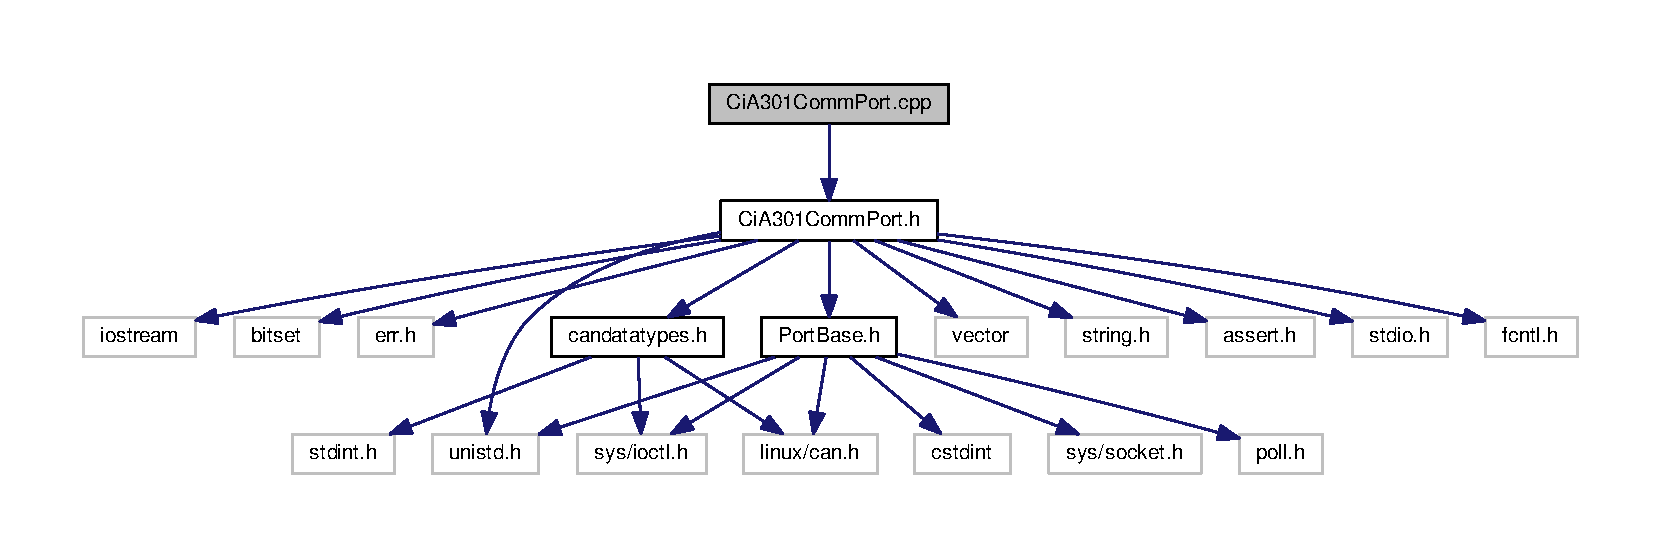
\includegraphics[width=350pt]{CiA301CommPort_8cpp__incl}
\end{center}
\end{figure}

\hypertarget{CiA301CommPort_8h}{}\section{Ci\+A301\+Comm\+Port.\+h File Reference}
\label{CiA301CommPort_8h}\index{Ci\+A301\+Comm\+Port.\+h@{Ci\+A301\+Comm\+Port.\+h}}
{\ttfamily \#include $<$iostream$>$}\\*
{\ttfamily \#include $<$bitset$>$}\\*
{\ttfamily \#include $<$err.\+h$>$}\\*
{\ttfamily \#include $<$unistd.\+h$>$}\\*
{\ttfamily \#include $<$vector$>$}\\*
{\ttfamily \#include $<$string.\+h$>$}\\*
{\ttfamily \#include $<$assert.\+h$>$}\\*
{\ttfamily \#include $<$stdio.\+h$>$}\\*
{\ttfamily \#include $<$fcntl.\+h$>$}\\*
{\ttfamily \#include \char`\"{}candatatypes.\+h\char`\"{}}\\*
{\ttfamily \#include \char`\"{}Port\+Base.\+h\char`\"{}}\\*
Include dependency graph for Ci\+A301\+Comm\+Port.\+h\+:
\nopagebreak
\begin{figure}[H]
\begin{center}
\leavevmode
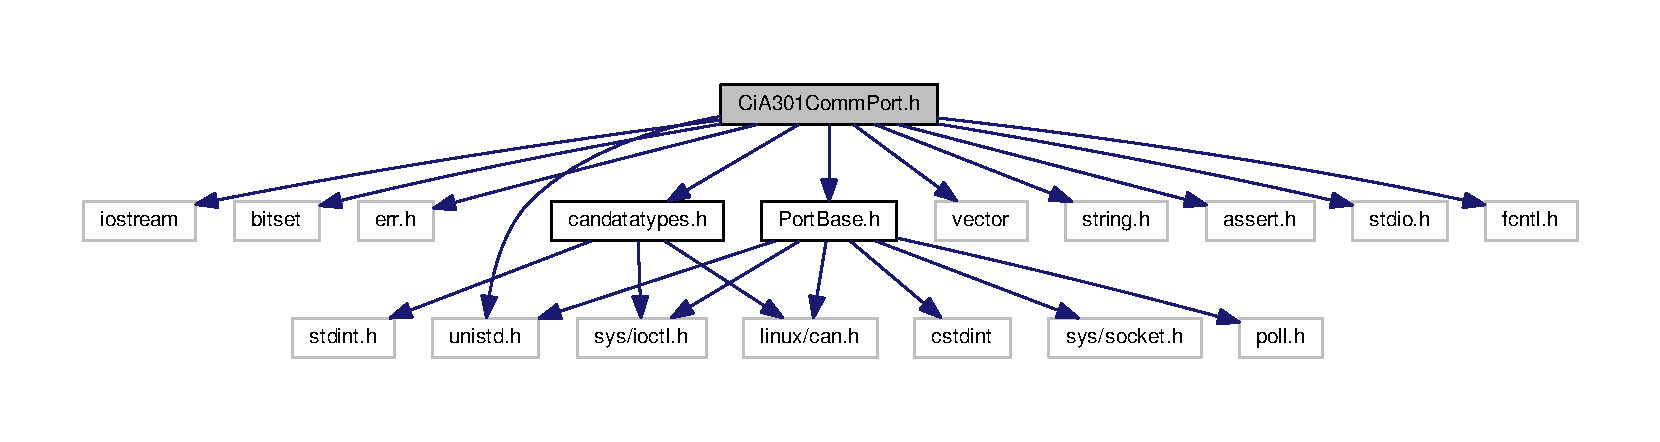
\includegraphics[width=350pt]{CiA301CommPort_8h__incl}
\end{center}
\end{figure}
This graph shows which files directly or indirectly include this file\+:
\nopagebreak
\begin{figure}[H]
\begin{center}
\leavevmode
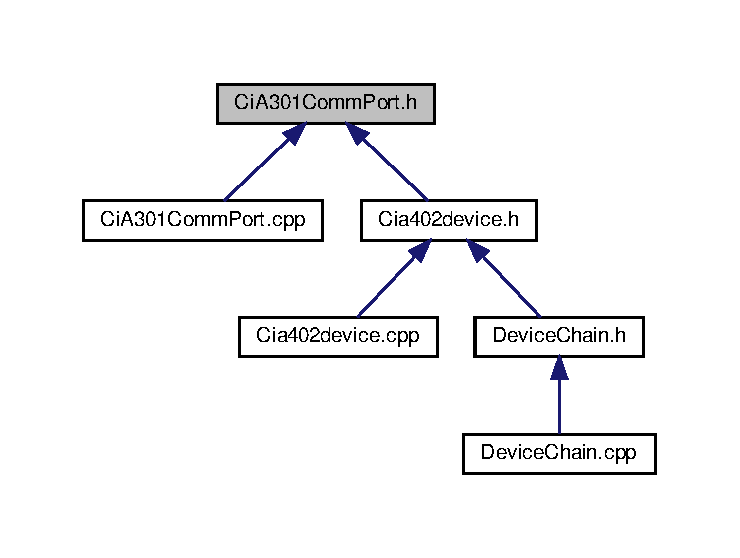
\includegraphics[width=350pt]{CiA301CommPort_8h__dep__incl}
\end{center}
\end{figure}
\subsection*{Classes}
\begin{DoxyCompactItemize}
\item 
class \hyperlink{classCiA301CommPort}{Ci\+A301\+Comm\+Port}
\end{DoxyCompactItemize}
\subsection*{Namespaces}
\begin{DoxyCompactItemize}
\item 
 \hyperlink{namespacesdo}{sdo}
\item 
 \hyperlink{namespacepdo}{pdo}
\item 
 \hyperlink{namespacenmt}{nmt}
\end{DoxyCompactItemize}
\subsection*{Macros}
\begin{DoxyCompactItemize}
\item 
\#define \hyperlink{CiA301CommPort_8h_a9c4538b32717c71448f328bccbf80784}{U\+S\+E\+\_\+\+T\+I\+M\+E\+O\+UT}~200
\item 
\#define \hyperlink{CiA301CommPort_8h_a1ac42c9168b067855b5bb1e8e96afb62}{F\+I\+N\+D\+\_\+\+R\+E\+T\+RY}~20
\end{DoxyCompactItemize}
\subsection*{Variables}
\begin{DoxyCompactItemize}
\item 
const uint16\+\_\+t \hyperlink{namespacesdo_ada4eb9ed2535da14a1b4c449b52c98b6}{sdo\+::tx0} =0x580
\item 
const uint16\+\_\+t \hyperlink{namespacesdo_a32e87699bc0a4deed591fb38703c48f2}{sdo\+::rx0} =0x600
\item 
const uint16\+\_\+t \hyperlink{namespacepdo_a4a8e678f87bbe2520c5cffe3f6a6dae0}{pdo\+::tx0} =0x180
\item 
const uint16\+\_\+t \hyperlink{namespacepdo_a3a8ecb285207c4eb0b05bc69762404cf}{pdo\+::rx0} =0x200
\item 
const uint16\+\_\+t \hyperlink{namespacepdo_ae5f87d5007685cfd9d219e1cb051ccf0}{pdo\+::tx1} =0x280
\item 
const uint16\+\_\+t \hyperlink{namespacepdo_a1388fefc691ccce0ef2ea8347f737d1d}{pdo\+::rx1} =0x300
\item 
const uint16\+\_\+t \hyperlink{namespacepdo_a12b62b143e83e83b2566dea6d20a169a}{pdo\+::tx4} =0x380
\item 
const uint16\+\_\+t \hyperlink{namespacepdo_ab45e1d027abca75c1d406d514d3f6085}{pdo\+::rx4} =0x400
\item 
const vector$<$ uint8\+\_\+t $>$ \hyperlink{namespacenmt_a1310e5c59553352490180a42ef1dad8c}{nmt\+::started} =\{0x01\}
\end{DoxyCompactItemize}


\subsection{Macro Definition Documentation}
\index{Ci\+A301\+Comm\+Port.\+h@{Ci\+A301\+Comm\+Port.\+h}!F\+I\+N\+D\+\_\+\+R\+E\+T\+RY@{F\+I\+N\+D\+\_\+\+R\+E\+T\+RY}}
\index{F\+I\+N\+D\+\_\+\+R\+E\+T\+RY@{F\+I\+N\+D\+\_\+\+R\+E\+T\+RY}!Ci\+A301\+Comm\+Port.\+h@{Ci\+A301\+Comm\+Port.\+h}}
\subsubsection[{\texorpdfstring{F\+I\+N\+D\+\_\+\+R\+E\+T\+RY}{FIND_RETRY}}]{\setlength{\rightskip}{0pt plus 5cm}\#define F\+I\+N\+D\+\_\+\+R\+E\+T\+RY~20}\hypertarget{CiA301CommPort_8h_a1ac42c9168b067855b5bb1e8e96afb62}{}\label{CiA301CommPort_8h_a1ac42c9168b067855b5bb1e8e96afb62}
\index{Ci\+A301\+Comm\+Port.\+h@{Ci\+A301\+Comm\+Port.\+h}!U\+S\+E\+\_\+\+T\+I\+M\+E\+O\+UT@{U\+S\+E\+\_\+\+T\+I\+M\+E\+O\+UT}}
\index{U\+S\+E\+\_\+\+T\+I\+M\+E\+O\+UT@{U\+S\+E\+\_\+\+T\+I\+M\+E\+O\+UT}!Ci\+A301\+Comm\+Port.\+h@{Ci\+A301\+Comm\+Port.\+h}}
\subsubsection[{\texorpdfstring{U\+S\+E\+\_\+\+T\+I\+M\+E\+O\+UT}{USE_TIMEOUT}}]{\setlength{\rightskip}{0pt plus 5cm}\#define U\+S\+E\+\_\+\+T\+I\+M\+E\+O\+UT~200}\hypertarget{CiA301CommPort_8h_a9c4538b32717c71448f328bccbf80784}{}\label{CiA301CommPort_8h_a9c4538b32717c71448f328bccbf80784}

\hypertarget{Cia402device_8cpp}{}\section{Cia402device.\+cpp File Reference}
\label{Cia402device_8cpp}\index{Cia402device.\+cpp@{Cia402device.\+cpp}}
{\ttfamily \#include \char`\"{}Cia402device.\+h\char`\"{}}\\*
Include dependency graph for Cia402device.\+cpp\+:
\nopagebreak
\begin{figure}[H]
\begin{center}
\leavevmode
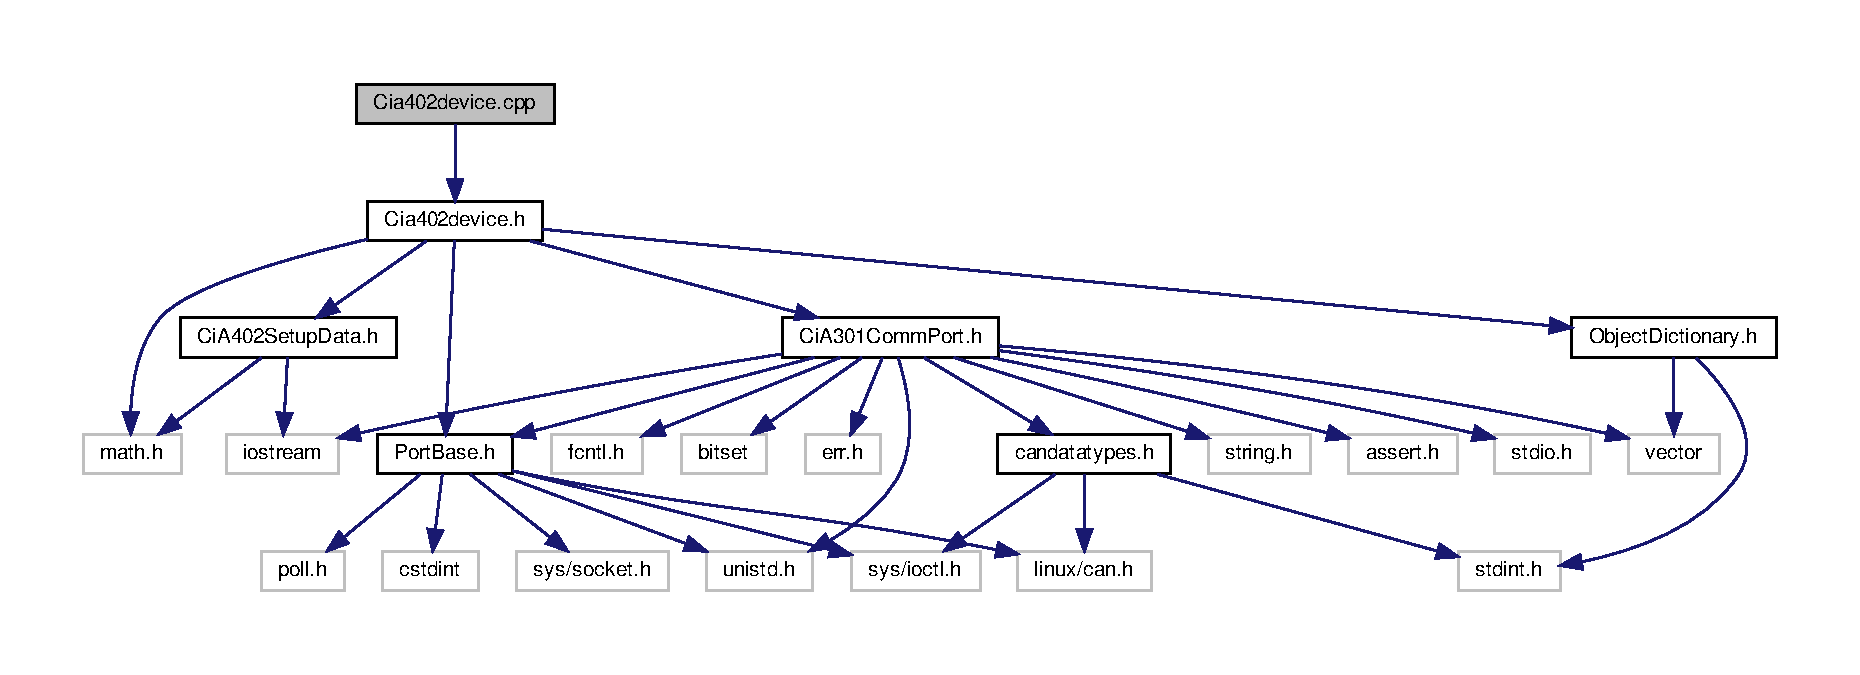
\includegraphics[width=350pt]{Cia402device_8cpp__incl}
\end{center}
\end{figure}
\subsection*{Functions}
\begin{DoxyCompactItemize}
\item 
vector$<$ uint8\+\_\+t $>$ \hyperlink{Cia402device_8cpp_ae234205c3014b4a69b38fff2c9602132}{data32to4x8} (uint32\+\_\+t in)
\item 
vector$<$ uint8\+\_\+t $>$ \hyperlink{Cia402device_8cpp_ab66ff1d3349b2b4fb19ffe21e8b1269a}{data16to2x8} (uint16\+\_\+t in)
\end{DoxyCompactItemize}


\subsection{Function Documentation}
\index{Cia402device.\+cpp@{Cia402device.\+cpp}!data16to2x8@{data16to2x8}}
\index{data16to2x8@{data16to2x8}!Cia402device.\+cpp@{Cia402device.\+cpp}}
\subsubsection[{\texorpdfstring{data16to2x8(uint16\+\_\+t in)}{data16to2x8(uint16_t in)}}]{\setlength{\rightskip}{0pt plus 5cm}vector$<$ uint8\+\_\+t $>$ data16to2x8 (
\begin{DoxyParamCaption}
\item[{uint16\+\_\+t}]{in}
\end{DoxyParamCaption}
)}\hypertarget{Cia402device_8cpp_ab66ff1d3349b2b4fb19ffe21e8b1269a}{}\label{Cia402device_8cpp_ab66ff1d3349b2b4fb19ffe21e8b1269a}
\index{Cia402device.\+cpp@{Cia402device.\+cpp}!data32to4x8@{data32to4x8}}
\index{data32to4x8@{data32to4x8}!Cia402device.\+cpp@{Cia402device.\+cpp}}
\subsubsection[{\texorpdfstring{data32to4x8(uint32\+\_\+t in)}{data32to4x8(uint32_t in)}}]{\setlength{\rightskip}{0pt plus 5cm}vector$<$ uint8\+\_\+t $>$ data32to4x8 (
\begin{DoxyParamCaption}
\item[{uint32\+\_\+t}]{in}
\end{DoxyParamCaption}
)}\hypertarget{Cia402device_8cpp_ae234205c3014b4a69b38fff2c9602132}{}\label{Cia402device_8cpp_ae234205c3014b4a69b38fff2c9602132}

\hypertarget{Cia402device_8h}{}\section{Cia402device.\+h File Reference}
\label{Cia402device_8h}\index{Cia402device.\+h@{Cia402device.\+h}}
{\ttfamily \#include $<$chrono$>$}\\*
{\ttfamily \#include $<$thread$>$}\\*
{\ttfamily \#include $<$math.\+h$>$}\\*
{\ttfamily \#include \char`\"{}Ci\+A301\+Comm\+Port.\+h\char`\"{}}\\*
{\ttfamily \#include \char`\"{}Object\+Dictionary.\+h\char`\"{}}\\*
{\ttfamily \#include \char`\"{}Port\+Base.\+h\char`\"{}}\\*
{\ttfamily \#include \char`\"{}Ci\+A402\+Setup\+Data.\+h\char`\"{}}\\*
Include dependency graph for Cia402device.\+h\+:
\nopagebreak
\begin{figure}[H]
\begin{center}
\leavevmode
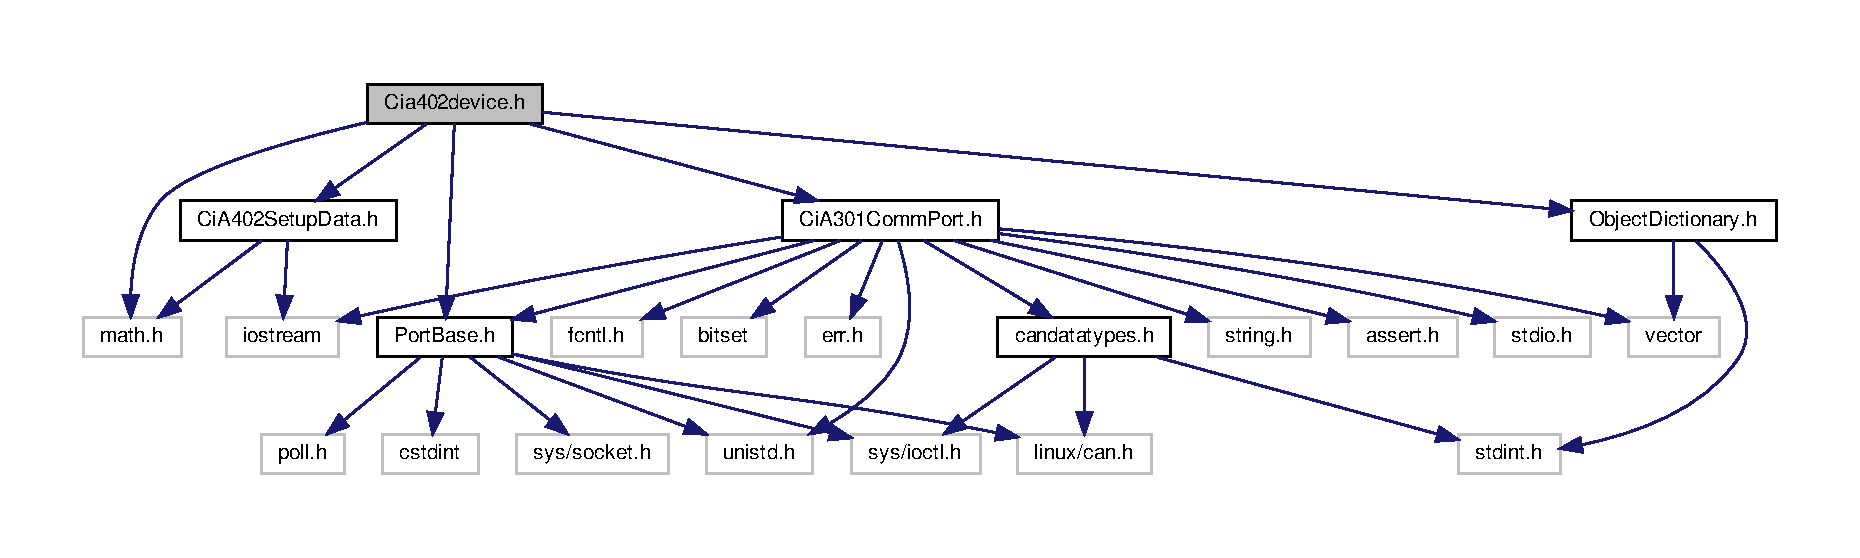
\includegraphics[width=350pt]{Cia402device_8h__incl}
\end{center}
\end{figure}
This graph shows which files directly or indirectly include this file\+:
\nopagebreak
\begin{figure}[H]
\begin{center}
\leavevmode
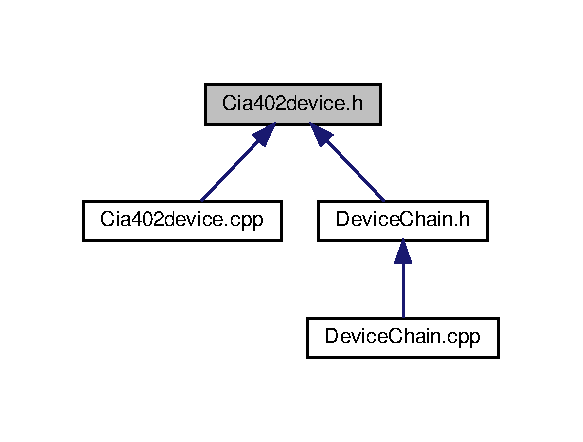
\includegraphics[width=280pt]{Cia402device_8h__dep__incl}
\end{center}
\end{figure}
\subsection*{Classes}
\begin{DoxyCompactItemize}
\item 
class \hyperlink{classCiA402Device}{Ci\+A402\+Device}
\end{DoxyCompactItemize}
\subsection*{Macros}
\begin{DoxyCompactItemize}
\item 
\#define \hyperlink{Cia402device_8h_a598a3330b3c21701223ee0ca14316eca}{PI}~3.\+14159265358
\item 
\#define \hyperlink{Cia402device_8h_ad40c559411b96d7cb25cddea2597917f}{R\+P\+M2\+R\+A\+DS}~(2.\+0$\ast$\hyperlink{Cia402device_8h_a598a3330b3c21701223ee0ca14316eca}{PI})/60.\+0
\item 
\#define \hyperlink{Cia402device_8h_afac1cb3c0e5f8e76953d71e525c85b5a}{R\+A\+D\+S2\+R\+PM}~60.\+0/(2.\+0$\ast$\hyperlink{Cia402device_8h_a598a3330b3c21701223ee0ca14316eca}{PI})
\item 
\#define \hyperlink{Cia402device_8h_ad39cd73edfd605f860349ff73aa1f0e1}{D\+E\+G2\+R\+A\+DS}~(2.\+0$\ast$\hyperlink{Cia402device_8h_a598a3330b3c21701223ee0ca14316eca}{PI})/360.\+0
\item 
\#define \hyperlink{Cia402device_8h_a445fa46f44fdc878f2653874a83cab73}{R\+A\+D\+S2\+D\+EG}~360.\+0/(2.\+0$\ast$\hyperlink{Cia402device_8h_a598a3330b3c21701223ee0ca14316eca}{PI})
\item 
\#define \hyperlink{Cia402device_8h_afa8cb3c12dbeaa9561ce45e7af88636f}{H\+I\+G\+H\+P\+A\+R\+T\+\_\+\+B\+I\+T\+S\+H\+I\+F\+T\+\_\+16}~0x10000
\item 
\#define \hyperlink{Cia402device_8h_a7c21d01106152feef7a4acd77afe01ae}{A\+N\+A\+L\+O\+G\+U\+E\+\_\+\+I\+N\+P\+U\+T\+\_\+\+S\+C\+A\+LE}~0x\+F\+F\+F0
\end{DoxyCompactItemize}


\subsection{Macro Definition Documentation}
\index{Cia402device.\+h@{Cia402device.\+h}!A\+N\+A\+L\+O\+G\+U\+E\+\_\+\+I\+N\+P\+U\+T\+\_\+\+S\+C\+A\+LE@{A\+N\+A\+L\+O\+G\+U\+E\+\_\+\+I\+N\+P\+U\+T\+\_\+\+S\+C\+A\+LE}}
\index{A\+N\+A\+L\+O\+G\+U\+E\+\_\+\+I\+N\+P\+U\+T\+\_\+\+S\+C\+A\+LE@{A\+N\+A\+L\+O\+G\+U\+E\+\_\+\+I\+N\+P\+U\+T\+\_\+\+S\+C\+A\+LE}!Cia402device.\+h@{Cia402device.\+h}}
\subsubsection[{\texorpdfstring{A\+N\+A\+L\+O\+G\+U\+E\+\_\+\+I\+N\+P\+U\+T\+\_\+\+S\+C\+A\+LE}{ANALOGUE_INPUT_SCALE}}]{\setlength{\rightskip}{0pt plus 5cm}\#define A\+N\+A\+L\+O\+G\+U\+E\+\_\+\+I\+N\+P\+U\+T\+\_\+\+S\+C\+A\+LE~0x\+F\+F\+F0}\hypertarget{Cia402device_8h_a7c21d01106152feef7a4acd77afe01ae}{}\label{Cia402device_8h_a7c21d01106152feef7a4acd77afe01ae}
\index{Cia402device.\+h@{Cia402device.\+h}!D\+E\+G2\+R\+A\+DS@{D\+E\+G2\+R\+A\+DS}}
\index{D\+E\+G2\+R\+A\+DS@{D\+E\+G2\+R\+A\+DS}!Cia402device.\+h@{Cia402device.\+h}}
\subsubsection[{\texorpdfstring{D\+E\+G2\+R\+A\+DS}{DEG2RADS}}]{\setlength{\rightskip}{0pt plus 5cm}\#define D\+E\+G2\+R\+A\+DS~(2.\+0$\ast${\bf PI})/360.\+0}\hypertarget{Cia402device_8h_ad39cd73edfd605f860349ff73aa1f0e1}{}\label{Cia402device_8h_ad39cd73edfd605f860349ff73aa1f0e1}
\index{Cia402device.\+h@{Cia402device.\+h}!H\+I\+G\+H\+P\+A\+R\+T\+\_\+\+B\+I\+T\+S\+H\+I\+F\+T\+\_\+16@{H\+I\+G\+H\+P\+A\+R\+T\+\_\+\+B\+I\+T\+S\+H\+I\+F\+T\+\_\+16}}
\index{H\+I\+G\+H\+P\+A\+R\+T\+\_\+\+B\+I\+T\+S\+H\+I\+F\+T\+\_\+16@{H\+I\+G\+H\+P\+A\+R\+T\+\_\+\+B\+I\+T\+S\+H\+I\+F\+T\+\_\+16}!Cia402device.\+h@{Cia402device.\+h}}
\subsubsection[{\texorpdfstring{H\+I\+G\+H\+P\+A\+R\+T\+\_\+\+B\+I\+T\+S\+H\+I\+F\+T\+\_\+16}{HIGHPART_BITSHIFT_16}}]{\setlength{\rightskip}{0pt plus 5cm}\#define H\+I\+G\+H\+P\+A\+R\+T\+\_\+\+B\+I\+T\+S\+H\+I\+F\+T\+\_\+16~0x10000}\hypertarget{Cia402device_8h_afa8cb3c12dbeaa9561ce45e7af88636f}{}\label{Cia402device_8h_afa8cb3c12dbeaa9561ce45e7af88636f}
\index{Cia402device.\+h@{Cia402device.\+h}!PI@{PI}}
\index{PI@{PI}!Cia402device.\+h@{Cia402device.\+h}}
\subsubsection[{\texorpdfstring{PI}{PI}}]{\setlength{\rightskip}{0pt plus 5cm}\#define PI~3.\+14159265358}\hypertarget{Cia402device_8h_a598a3330b3c21701223ee0ca14316eca}{}\label{Cia402device_8h_a598a3330b3c21701223ee0ca14316eca}
\index{Cia402device.\+h@{Cia402device.\+h}!R\+A\+D\+S2\+D\+EG@{R\+A\+D\+S2\+D\+EG}}
\index{R\+A\+D\+S2\+D\+EG@{R\+A\+D\+S2\+D\+EG}!Cia402device.\+h@{Cia402device.\+h}}
\subsubsection[{\texorpdfstring{R\+A\+D\+S2\+D\+EG}{RADS2DEG}}]{\setlength{\rightskip}{0pt plus 5cm}\#define R\+A\+D\+S2\+D\+EG~360.\+0/(2.\+0$\ast${\bf PI})}\hypertarget{Cia402device_8h_a445fa46f44fdc878f2653874a83cab73}{}\label{Cia402device_8h_a445fa46f44fdc878f2653874a83cab73}
\index{Cia402device.\+h@{Cia402device.\+h}!R\+A\+D\+S2\+R\+PM@{R\+A\+D\+S2\+R\+PM}}
\index{R\+A\+D\+S2\+R\+PM@{R\+A\+D\+S2\+R\+PM}!Cia402device.\+h@{Cia402device.\+h}}
\subsubsection[{\texorpdfstring{R\+A\+D\+S2\+R\+PM}{RADS2RPM}}]{\setlength{\rightskip}{0pt plus 5cm}\#define R\+A\+D\+S2\+R\+PM~60.\+0/(2.\+0$\ast${\bf PI})}\hypertarget{Cia402device_8h_afac1cb3c0e5f8e76953d71e525c85b5a}{}\label{Cia402device_8h_afac1cb3c0e5f8e76953d71e525c85b5a}
\index{Cia402device.\+h@{Cia402device.\+h}!R\+P\+M2\+R\+A\+DS@{R\+P\+M2\+R\+A\+DS}}
\index{R\+P\+M2\+R\+A\+DS@{R\+P\+M2\+R\+A\+DS}!Cia402device.\+h@{Cia402device.\+h}}
\subsubsection[{\texorpdfstring{R\+P\+M2\+R\+A\+DS}{RPM2RADS}}]{\setlength{\rightskip}{0pt plus 5cm}\#define R\+P\+M2\+R\+A\+DS~(2.\+0$\ast${\bf PI})/60.\+0}\hypertarget{Cia402device_8h_ad40c559411b96d7cb25cddea2597917f}{}\label{Cia402device_8h_ad40c559411b96d7cb25cddea2597917f}

\hypertarget{CiA402DeviceICanbus_8cpp}{}\section{Ci\+A402\+Device\+I\+Canbus.\+cpp File Reference}
\label{CiA402DeviceICanbus_8cpp}\index{Ci\+A402\+Device\+I\+Canbus.\+cpp@{Ci\+A402\+Device\+I\+Canbus.\+cpp}}
{\ttfamily \#include \char`\"{}Ci\+A402\+Device\+I\+Canbus.\+h\char`\"{}}\\*
Include dependency graph for Ci\+A402\+Device\+I\+Canbus.\+cpp\+:
\nopagebreak
\begin{figure}[H]
\begin{center}
\leavevmode
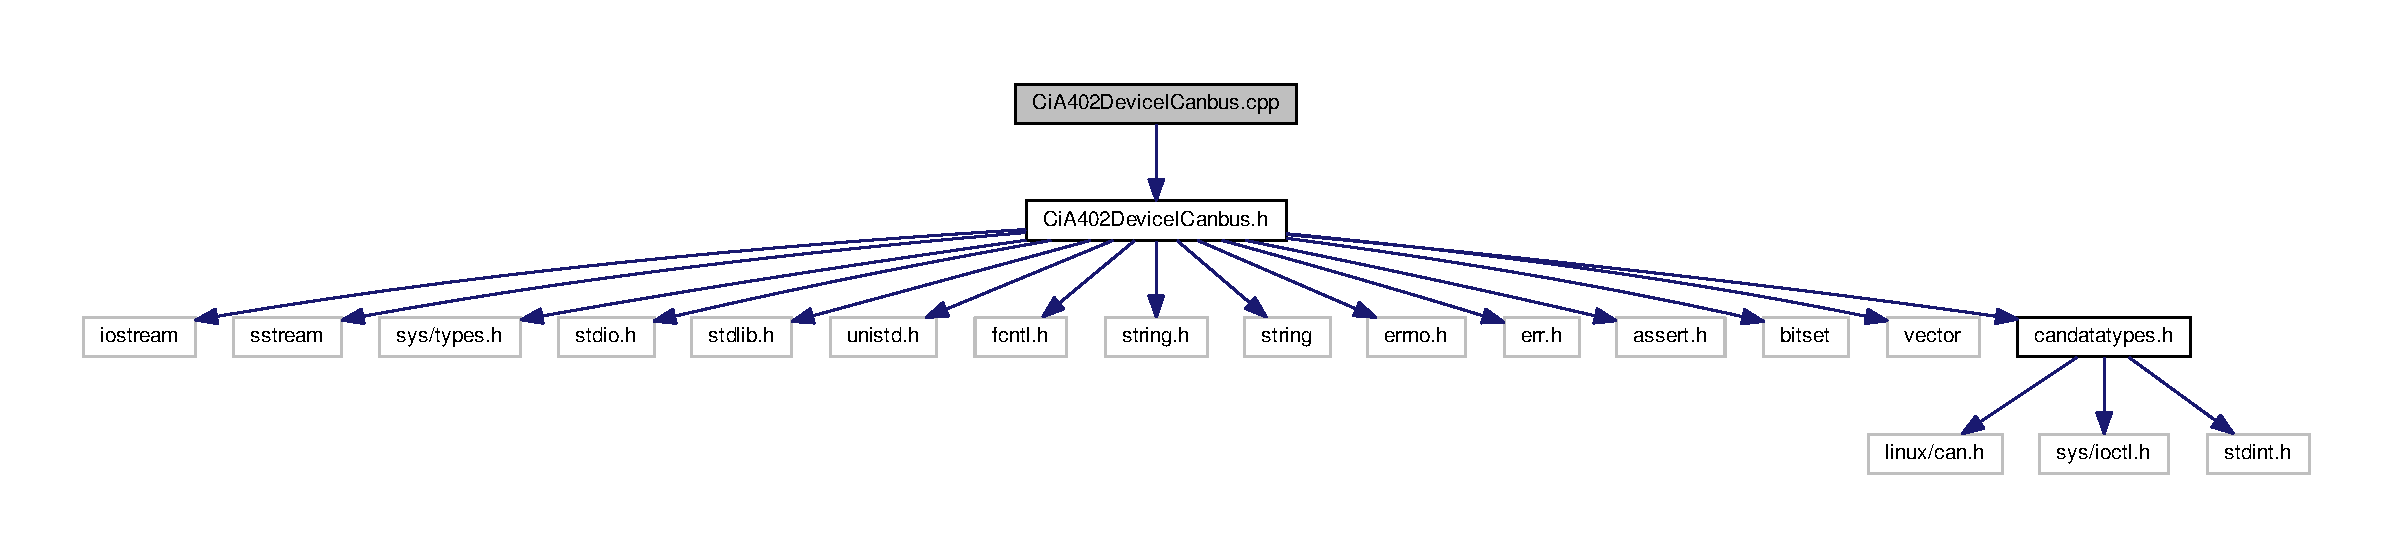
\includegraphics[width=350pt]{CiA402DeviceICanbus_8cpp__incl}
\end{center}
\end{figure}
\subsection*{Macros}
\begin{DoxyCompactItemize}
\item 
\#define \hyperlink{CiA402DeviceICanbus_8cpp_a9c4538b32717c71448f328bccbf80784}{U\+S\+E\+\_\+\+T\+I\+M\+E\+O\+UT}~200
\end{DoxyCompactItemize}


\subsection{Macro Definition Documentation}
\index{Ci\+A402\+Device\+I\+Canbus.\+cpp@{Ci\+A402\+Device\+I\+Canbus.\+cpp}!U\+S\+E\+\_\+\+T\+I\+M\+E\+O\+UT@{U\+S\+E\+\_\+\+T\+I\+M\+E\+O\+UT}}
\index{U\+S\+E\+\_\+\+T\+I\+M\+E\+O\+UT@{U\+S\+E\+\_\+\+T\+I\+M\+E\+O\+UT}!Ci\+A402\+Device\+I\+Canbus.\+cpp@{Ci\+A402\+Device\+I\+Canbus.\+cpp}}
\subsubsection[{\texorpdfstring{U\+S\+E\+\_\+\+T\+I\+M\+E\+O\+UT}{USE_TIMEOUT}}]{\setlength{\rightskip}{0pt plus 5cm}\#define U\+S\+E\+\_\+\+T\+I\+M\+E\+O\+UT~200}\hypertarget{CiA402DeviceICanbus_8cpp_a9c4538b32717c71448f328bccbf80784}{}\label{CiA402DeviceICanbus_8cpp_a9c4538b32717c71448f328bccbf80784}

\hypertarget{CiA402DeviceICanbus_8h}{}\section{Ci\+A402\+Device\+I\+Canbus.\+h File Reference}
\label{CiA402DeviceICanbus_8h}\index{Ci\+A402\+Device\+I\+Canbus.\+h@{Ci\+A402\+Device\+I\+Canbus.\+h}}
{\ttfamily \#include $<$iostream$>$}\\*
{\ttfamily \#include $<$sstream$>$}\\*
{\ttfamily \#include $<$sys/types.\+h$>$}\\*
{\ttfamily \#include $<$stdio.\+h$>$}\\*
{\ttfamily \#include $<$stdlib.\+h$>$}\\*
{\ttfamily \#include $<$unistd.\+h$>$}\\*
{\ttfamily \#include $<$fcntl.\+h$>$}\\*
{\ttfamily \#include $<$string.\+h$>$}\\*
{\ttfamily \#include $<$string$>$}\\*
{\ttfamily \#include $<$errno.\+h$>$}\\*
{\ttfamily \#include $<$err.\+h$>$}\\*
{\ttfamily \#include $<$assert.\+h$>$}\\*
{\ttfamily \#include $<$bitset$>$}\\*
{\ttfamily \#include $<$vector$>$}\\*
{\ttfamily \#include \char`\"{}candatatypes.\+h\char`\"{}}\\*
Include dependency graph for Ci\+A402\+Device\+I\+Canbus.\+h\+:
\nopagebreak
\begin{figure}[H]
\begin{center}
\leavevmode
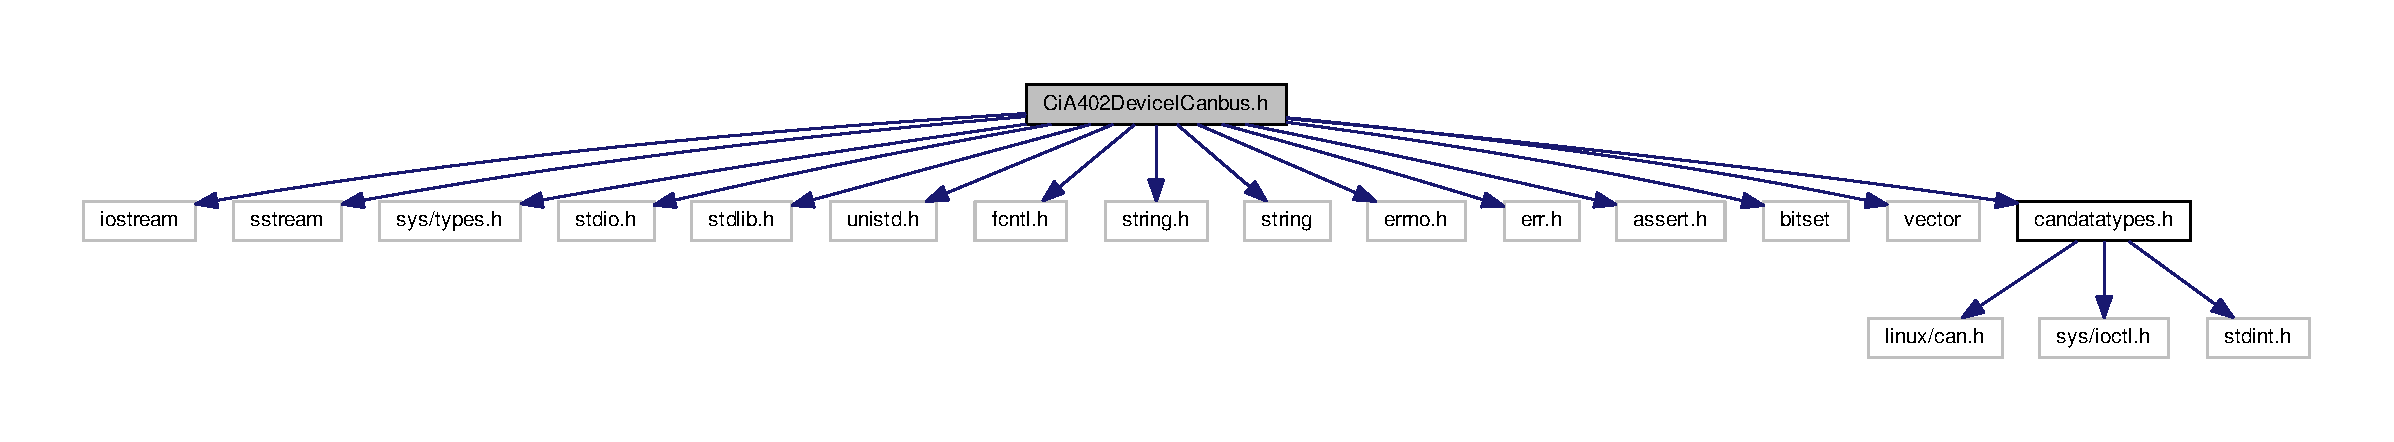
\includegraphics[width=350pt]{CiA402DeviceICanbus_8h__incl}
\end{center}
\end{figure}
This graph shows which files directly or indirectly include this file\+:
\nopagebreak
\begin{figure}[H]
\begin{center}
\leavevmode
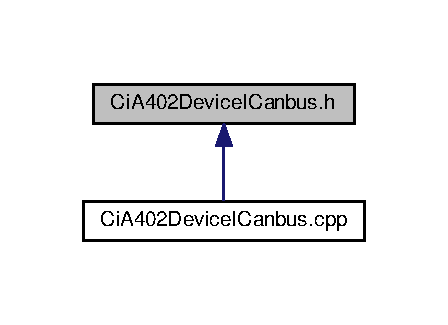
\includegraphics[width=215pt]{CiA402DeviceICanbus_8h__dep__incl}
\end{center}
\end{figure}
\subsection*{Classes}
\begin{DoxyCompactItemize}
\item 
class \hyperlink{classCiA402DeviceICanbus}{Ci\+A402\+Device\+I\+Canbus}
\end{DoxyCompactItemize}

\hypertarget{CiA402SetupData_8cpp}{}\section{Ci\+A402\+Setup\+Data.\+cpp File Reference}
\label{CiA402SetupData_8cpp}\index{Ci\+A402\+Setup\+Data.\+cpp@{Ci\+A402\+Setup\+Data.\+cpp}}
{\ttfamily \#include \char`\"{}Ci\+A402\+Setup\+Data.\+h\char`\"{}}\\*
Include dependency graph for Ci\+A402\+Setup\+Data.\+cpp\+:
\nopagebreak
\begin{figure}[H]
\begin{center}
\leavevmode
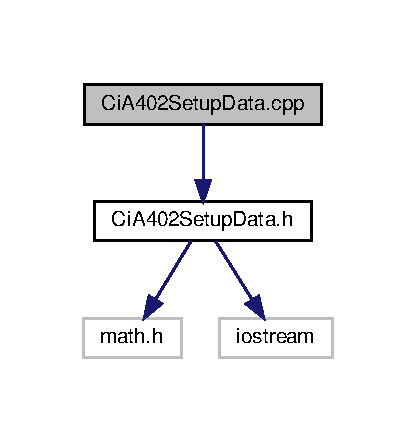
\includegraphics[width=200pt]{CiA402SetupData_8cpp__incl}
\end{center}
\end{figure}

\hypertarget{CiA402SetupData_8h}{}\section{Ci\+A402\+Setup\+Data.\+h File Reference}
\label{CiA402SetupData_8h}\index{Ci\+A402\+Setup\+Data.\+h@{Ci\+A402\+Setup\+Data.\+h}}
{\ttfamily \#include $<$math.\+h$>$}\\*
{\ttfamily \#include $<$iostream$>$}\\*
Include dependency graph for Ci\+A402\+Setup\+Data.\+h\+:
\nopagebreak
\begin{figure}[H]
\begin{center}
\leavevmode
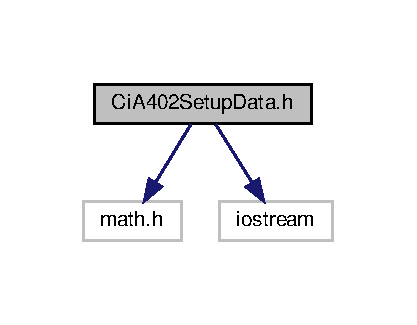
\includegraphics[width=200pt]{CiA402SetupData_8h__incl}
\end{center}
\end{figure}
This graph shows which files directly or indirectly include this file\+:
\nopagebreak
\begin{figure}[H]
\begin{center}
\leavevmode
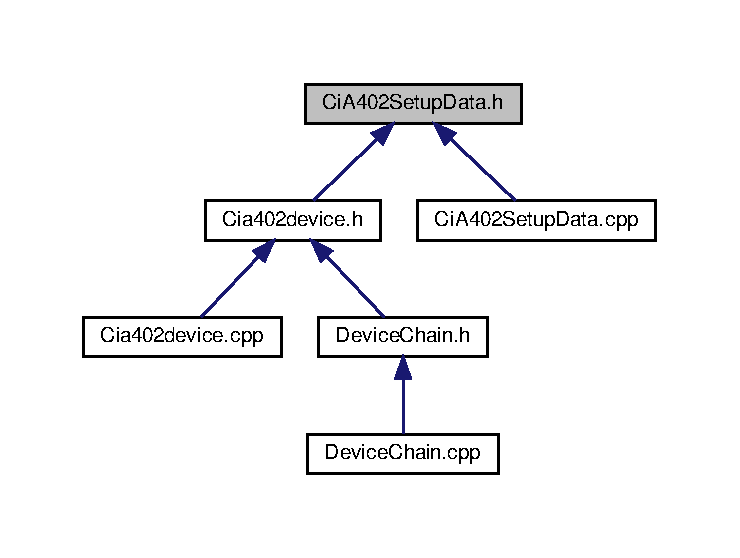
\includegraphics[width=350pt]{CiA402SetupData_8h__dep__incl}
\end{center}
\end{figure}
\subsection*{Classes}
\begin{DoxyCompactItemize}
\item 
class \hyperlink{classCiA402SetupData}{Ci\+A402\+Setup\+Data}
\end{DoxyCompactItemize}

\hypertarget{CMakeLists_8txt}{}\section{C\+Make\+Lists.\+txt File Reference}
\label{CMakeLists_8txt}\index{C\+Make\+Lists.\+txt@{C\+Make\+Lists.\+txt}}
\subsection*{Functions}
\begin{DoxyCompactItemize}
\item 
\hyperlink{CMakeLists_8txt_ac00329544182cb5a80fe0e1680f32cce}{project} (\hyperlink{classCiA402Device}{Ci\+A402\+Device}) add\+\_\+definitions(-\/D\+H\+I\+C\+O\+\_\+\+LE) aux\+\_\+source\+\_\+directory(.Ci\+A402\+Device\+\_\+\+S\+R\+CS) set(S\+U\+B\+D\+I\+R\+\_\+\+I\+N\+C\+L\+U\+D\+E\+\_\+\+D\+I\+R\+E\+C\+T\+O\+R\+I\+ES \$
\end{DoxyCompactItemize}


\subsection{Function Documentation}
\index{C\+Make\+Lists.\+txt@{C\+Make\+Lists.\+txt}!project@{project}}
\index{project@{project}!C\+Make\+Lists.\+txt@{C\+Make\+Lists.\+txt}}
\subsubsection[{\texorpdfstring{project(\+Ci\+A402\+Device) add\+\_\+definitions(-\/\+D\+H\+I\+C\+O\+\_\+\+L\+E) aux\+\_\+source\+\_\+directory(.\+Ci\+A402\+Device\+\_\+\+S\+R\+C\+S) set(\+S\+U\+B\+D\+I\+R\+\_\+\+I\+N\+C\+L\+U\+D\+E\+\_\+\+D\+I\+R\+E\+C\+T\+O\+R\+I\+E\+S \$}{project(CiA402Device) add_definitions(-DHICO_LE) aux_source_directory(.CiA402Device_SRCS) set(SUBDIR_INCLUDE_DIRECTORIES $}}]{\setlength{\rightskip}{0pt plus 5cm}project (
\begin{DoxyParamCaption}
\item[{{\bf Ci\+A402\+Device}}]{}
\end{DoxyParamCaption}
)}\hypertarget{CMakeLists_8txt_ac00329544182cb5a80fe0e1680f32cce}{}\label{CMakeLists_8txt_ac00329544182cb5a80fe0e1680f32cce}

\hypertarget{co__msg_8h}{}\section{co\+\_\+msg.\+h File Reference}
\label{co__msg_8h}\index{co\+\_\+msg.\+h@{co\+\_\+msg.\+h}}
\subsection*{Classes}
\begin{DoxyCompactItemize}
\item 
struct \hyperlink{structco__msg}{co\+\_\+msg}
\end{DoxyCompactItemize}

\hypertarget{DeviceChain_8cpp}{}\section{Device\+Chain.\+cpp File Reference}
\label{DeviceChain_8cpp}\index{Device\+Chain.\+cpp@{Device\+Chain.\+cpp}}
{\ttfamily \#include \char`\"{}Device\+Chain.\+h\char`\"{}}\\*
Include dependency graph for Device\+Chain.\+cpp\+:
\nopagebreak
\begin{figure}[H]
\begin{center}
\leavevmode
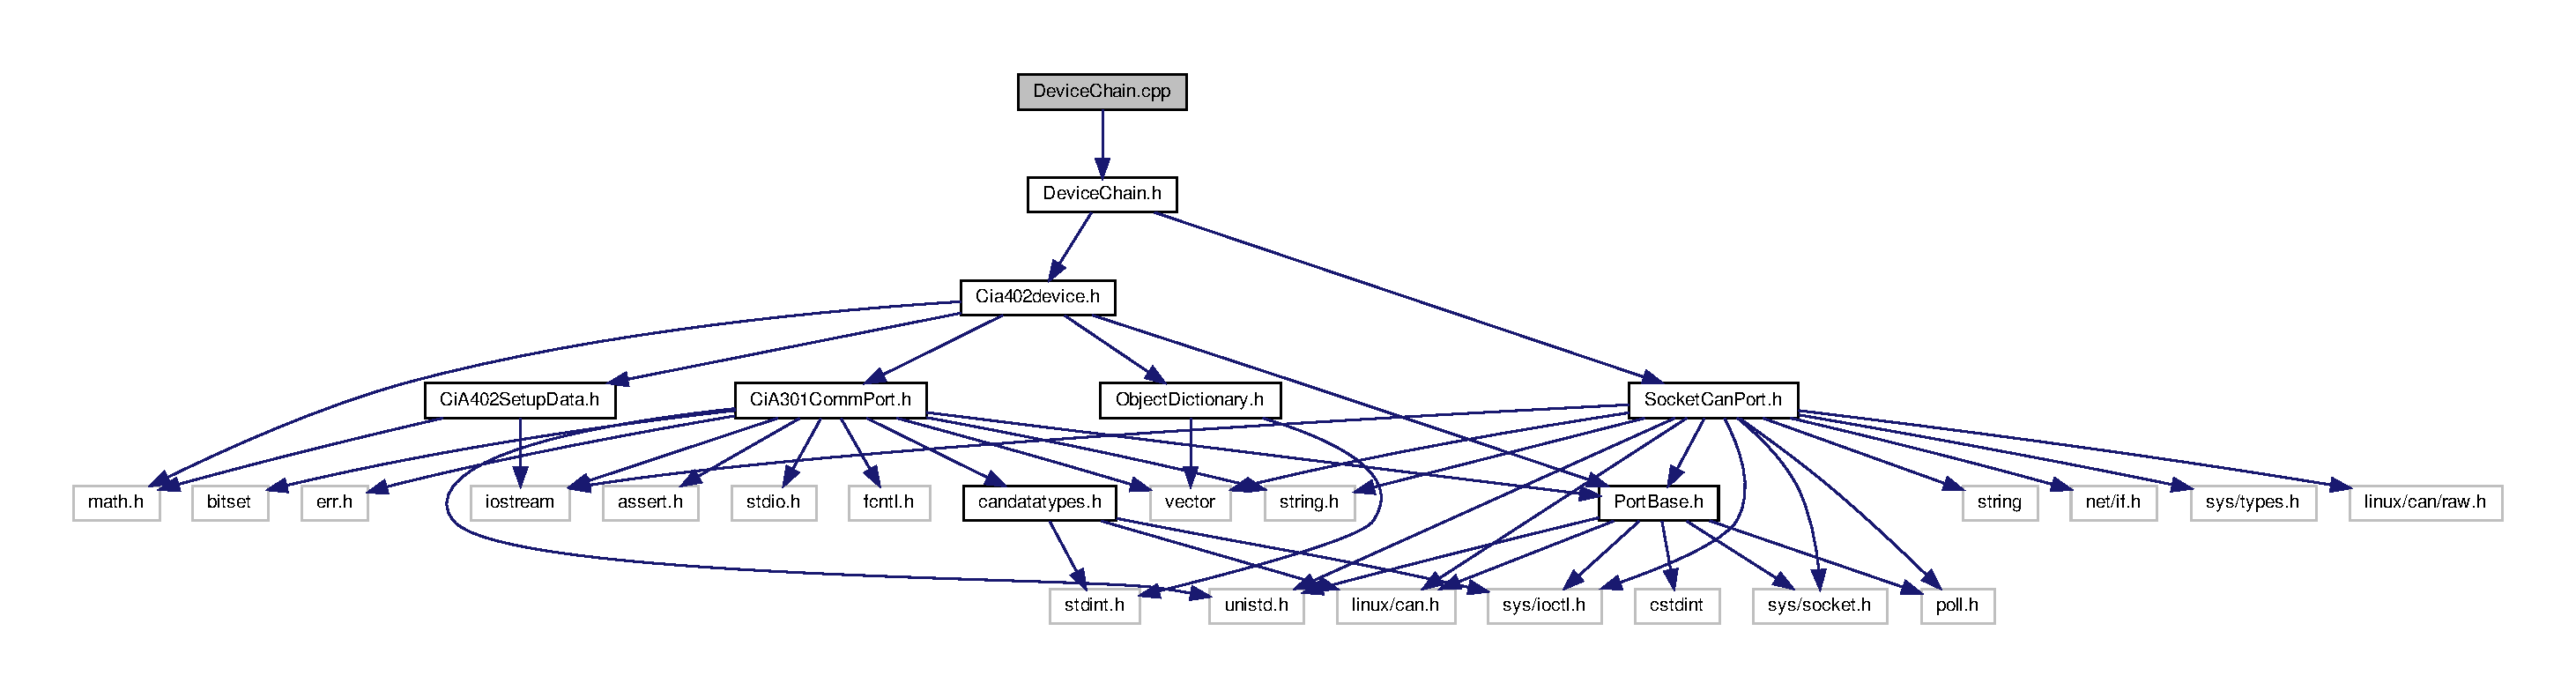
\includegraphics[width=350pt]{DeviceChain_8cpp__incl}
\end{center}
\end{figure}

\hypertarget{DeviceChain_8h}{}\section{Device\+Chain.\+h File Reference}
\label{DeviceChain_8h}\index{Device\+Chain.\+h@{Device\+Chain.\+h}}
{\ttfamily \#include \char`\"{}Cia402device.\+h\char`\"{}}\\*
{\ttfamily \#include \char`\"{}Socket\+Can\+Port.\+h\char`\"{}}\\*
Include dependency graph for Device\+Chain.\+h\+:
\nopagebreak
\begin{figure}[H]
\begin{center}
\leavevmode
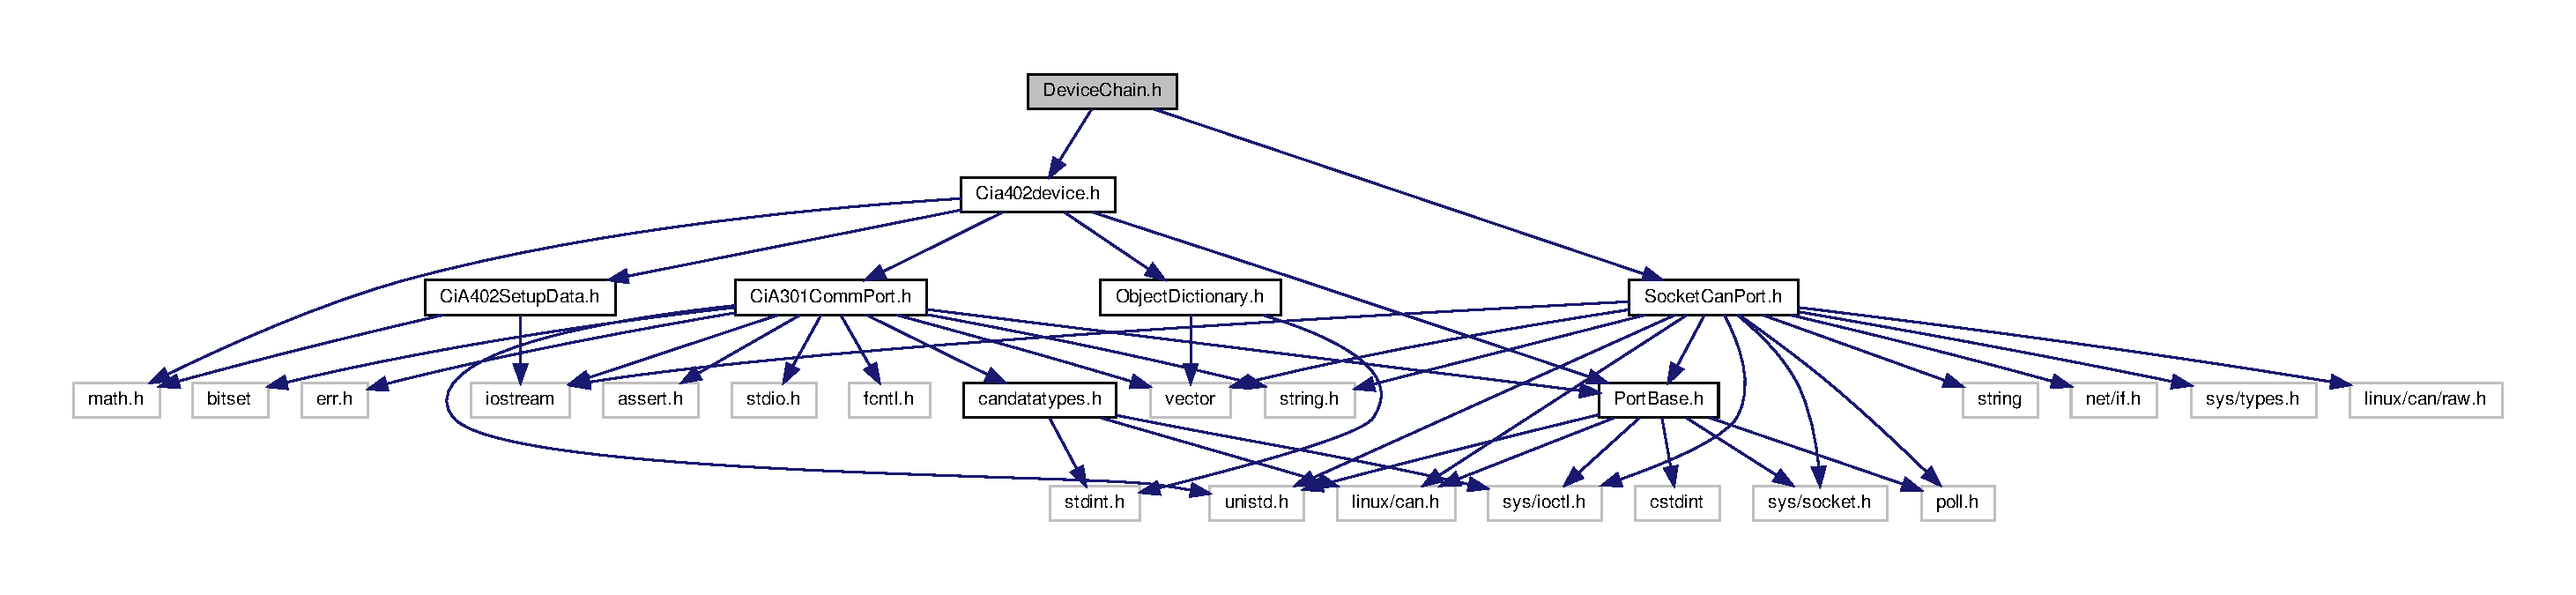
\includegraphics[width=350pt]{DeviceChain_8h__incl}
\end{center}
\end{figure}
This graph shows which files directly or indirectly include this file\+:
\nopagebreak
\begin{figure}[H]
\begin{center}
\leavevmode
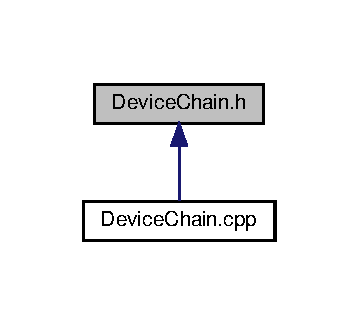
\includegraphics[width=172pt]{DeviceChain_8h__dep__incl}
\end{center}
\end{figure}
\subsection*{Classes}
\begin{DoxyCompactItemize}
\item 
class \hyperlink{classDeviceChain}{Device\+Chain}
\end{DoxyCompactItemize}

\hypertarget{hico__api_8h}{}\section{hico\+\_\+api.\+h File Reference}
\label{hico__api_8h}\index{hico\+\_\+api.\+h@{hico\+\_\+api.\+h}}
{\ttfamily \#include $<$sys/ioctl.\+h$>$}\\*
{\ttfamily \#include $<$stdint.\+h$>$}\\*
Include dependency graph for hico\+\_\+api.\+h\+:
\nopagebreak
\begin{figure}[H]
\begin{center}
\leavevmode
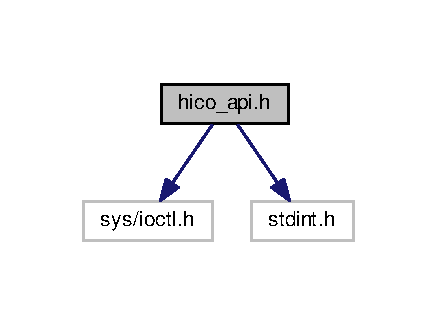
\includegraphics[width=210pt]{hico__api_8h__incl}
\end{center}
\end{figure}
\subsection*{Classes}
\begin{DoxyCompactItemize}
\item 
struct \hyperlink{structerr__stat}{err\+\_\+stat}
\item 
struct \hyperlink{structcan__msg}{can\+\_\+msg}
\item 
struct \hyperlink{structcan__filter}{can\+\_\+filter}
\end{DoxyCompactItemize}
\subsection*{Macros}
\begin{DoxyCompactItemize}
\item 
\#define \hyperlink{hico__api_8h_abb973a44d16fd02957aec9c47d5ac0b1}{I\+O\+C\+\_\+\+M\+A\+G\+IC}~\textquotesingle{}E\textquotesingle{}
\item 
\#define \hyperlink{hico__api_8h_a36d525cf4d116b2fe4ecc00222b256f1}{P\+A\+C\+K\+ED}~\+\_\+\+\_\+attribute\+\_\+\+\_\+((packed))
\item 
\#define \hyperlink{hico__api_8h_a2e1908762e3be59ff1f1249315817f3f}{I\+O\+C\+\_\+\+R\+E\+S\+E\+T\+\_\+\+B\+O\+A\+RD}~\+\_\+\+IO (\hyperlink{hico__api_8h_abb973a44d16fd02957aec9c47d5ac0b1}{I\+O\+C\+\_\+\+M\+A\+G\+IC}, 1)
\item 
\#define \hyperlink{hico__api_8h_a346da60de0bcf2ba4fe6d83c2439a6aa}{I\+O\+C\+\_\+\+S\+T\+A\+RT}~\+\_\+\+IO (\hyperlink{hico__api_8h_abb973a44d16fd02957aec9c47d5ac0b1}{I\+O\+C\+\_\+\+M\+A\+G\+IC}, 5)
\item 
\#define \hyperlink{hico__api_8h_a23b340dcb801bd677be094b1db214f21}{I\+O\+C\+\_\+\+S\+T\+A\+R\+T\+\_\+\+P\+A\+S\+S\+I\+VE}~\+\_\+\+IO (\hyperlink{hico__api_8h_abb973a44d16fd02957aec9c47d5ac0b1}{I\+O\+C\+\_\+\+M\+A\+G\+IC}, 10)
\item 
\#define \hyperlink{hico__api_8h_af8cda96f7edddada586e67abc795c9a7}{I\+O\+C\+\_\+\+S\+T\+A\+R\+T\+\_\+\+B\+A\+U\+D\+S\+C\+AN}~\+\_\+\+IO (\hyperlink{hico__api_8h_abb973a44d16fd02957aec9c47d5ac0b1}{I\+O\+C\+\_\+\+M\+A\+G\+IC}, 15)
\item 
\#define \hyperlink{hico__api_8h_a25a17d51ed18d29864905396e2542f2a}{I\+O\+C\+\_\+\+S\+T\+OP}~\+\_\+\+IO (\hyperlink{hico__api_8h_abb973a44d16fd02957aec9c47d5ac0b1}{I\+O\+C\+\_\+\+M\+A\+G\+IC}, 20)
\item 
\#define \hyperlink{hico__api_8h_a435f17e5332c2081e7ce09842664f183}{I\+O\+C\+\_\+\+G\+E\+T\+\_\+\+M\+O\+DE}~\+\_\+\+I\+OR(\hyperlink{hico__api_8h_abb973a44d16fd02957aec9c47d5ac0b1}{I\+O\+C\+\_\+\+M\+A\+G\+IC}, 25,  uint32\+\_\+t)
\item 
\#define \hyperlink{hico__api_8h_aff568c17dcaa5179a247a36874b011f6}{C\+M\+\_\+\+B\+A\+U\+D\+S\+C\+AN}~1
\item 
\#define \hyperlink{hico__api_8h_ac16bf18f66fbaf440f3dedf069a0f611}{C\+M\+\_\+\+P\+A\+S\+S\+I\+VE}~2
\item 
\#define \hyperlink{hico__api_8h_a6c1e851b693474b1b91bb0820adfbce3}{C\+M\+\_\+\+A\+C\+T\+I\+VE}~3
\item 
\#define \hyperlink{hico__api_8h_aa8bcd6538691e59322e8e3a03fad080a}{C\+M\+\_\+\+R\+E\+S\+ET}~4
\item 
\#define \hyperlink{hico__api_8h_a9bcc4d1b52c43e507f264eb3d326f1c5}{I\+O\+C\+\_\+\+S\+E\+T\+\_\+\+B\+I\+T\+R\+A\+TE}~\+\_\+\+I\+OW (\hyperlink{hico__api_8h_abb973a44d16fd02957aec9c47d5ac0b1}{I\+O\+C\+\_\+\+M\+A\+G\+IC}, 30, uint32\+\_\+t)
\item 
\#define \hyperlink{hico__api_8h_aa1ad7a89155a7f858ab52149c2fcaad5}{B\+I\+T\+R\+A\+T\+E\+\_\+10k}~0
\item 
\#define \hyperlink{hico__api_8h_a4eb46432ed1b9dd664fc642738a1a969}{B\+I\+T\+R\+A\+T\+E\+\_\+20k}~1
\item 
\#define \hyperlink{hico__api_8h_a39c91c0deb48d0a15d084f2a2021417b}{B\+I\+T\+R\+A\+T\+E\+\_\+50k}~2
\item 
\#define \hyperlink{hico__api_8h_aae6f862ae12a0da0d319cd353ea7befe}{B\+I\+T\+R\+A\+T\+E\+\_\+100k}~3
\item 
\#define \hyperlink{hico__api_8h_afbce0ed8bc362c29562f98ea81456e24}{B\+I\+T\+R\+A\+T\+E\+\_\+125k}~4
\item 
\#define \hyperlink{hico__api_8h_a634a59a9129b549f182844e7b4058a2a}{B\+I\+T\+R\+A\+T\+E\+\_\+250k}~5
\item 
\#define \hyperlink{hico__api_8h_a845bd49223fdabd4ebd206779eb8f3b1}{B\+I\+T\+R\+A\+T\+E\+\_\+500k}~6
\item 
\#define \hyperlink{hico__api_8h_a8b1930fb9b23dcba55143e0ef37081fc}{B\+I\+T\+R\+A\+T\+E\+\_\+800k}~7
\item 
\#define \hyperlink{hico__api_8h_a1432cd8532548faf2ae5287ca4a7413c}{B\+I\+T\+R\+A\+T\+E\+\_\+1000k}~8
\item 
\#define \hyperlink{hico__api_8h_a9b5344964c96f46fcfffc44074a499a5}{I\+O\+C\+\_\+\+S\+E\+T\+\_\+\+S\+J\+W\+\_\+\+I\+N\+C\+R\+E\+M\+E\+NT}~\+\_\+\+I\+OW (\hyperlink{hico__api_8h_abb973a44d16fd02957aec9c47d5ac0b1}{I\+O\+C\+\_\+\+M\+A\+G\+IC}, 31, uint32\+\_\+t)
\item 
\#define \hyperlink{hico__api_8h_a1be0497522ab2fd1aa5b9f7eaecda4fb}{I\+O\+C\+\_\+\+G\+E\+T\+\_\+\+B\+I\+T\+R\+A\+TE}~\+\_\+\+I\+OR (\hyperlink{hico__api_8h_abb973a44d16fd02957aec9c47d5ac0b1}{I\+O\+C\+\_\+\+M\+A\+G\+IC}, 35, uint32\+\_\+t)
\item 
\#define \hyperlink{hico__api_8h_ae59806663d8e8bfb7d05d5929367145b}{I\+O\+C\+\_\+\+G\+E\+T\+\_\+\+C\+A\+N\+\_\+\+S\+T\+A\+T\+US}~\+\_\+\+I\+OR (\hyperlink{hico__api_8h_abb973a44d16fd02957aec9c47d5ac0b1}{I\+O\+C\+\_\+\+M\+A\+G\+IC}, 40, uint32\+\_\+t)
\item 
\#define \hyperlink{hico__api_8h_a25c2242e25d7afcc48780b29b5894c19}{C\+S\+\_\+\+E\+R\+R\+O\+R\+\_\+\+P\+A\+S\+S\+I\+VE}~(1$<$$<$6)
\item 
\#define \hyperlink{hico__api_8h_a6778a854c562ab058773416c43135f40}{C\+S\+\_\+\+E\+R\+R\+O\+R\+\_\+\+B\+U\+S\+\_\+\+O\+FF}~(1$<$$<$7)
\item 
\#define \hyperlink{hico__api_8h_a351cedf4b15084ff51f4af74507dded1}{C\+S\+\_\+\+G\+E\+T\+\_\+\+R\+X\+E\+R\+R\+C\+NT}(status)~((status$>$$>$16)\&0xff)
\item 
\#define \hyperlink{hico__api_8h_af5d8a11d281bd10ef7c75547cd1fa0e1}{C\+S\+\_\+\+G\+E\+T\+\_\+\+T\+X\+E\+R\+R\+C\+NT}(status)~((status$>$$>$24)\&0xff)
\item 
\#define \hyperlink{hico__api_8h_a207812116166ed196307dd62a8737952}{I\+O\+C\+\_\+\+G\+E\+T\+\_\+\+B\+O\+A\+R\+D\+\_\+\+S\+T\+A\+T\+US}~\+\_\+\+I\+OR (\hyperlink{hico__api_8h_abb973a44d16fd02957aec9c47d5ac0b1}{I\+O\+C\+\_\+\+M\+A\+G\+IC}, 45, uint32\+\_\+t)
\item 
\#define \hyperlink{hico__api_8h_a8a1b833620a1a3e76e7ee3a8de419167}{B\+S\+\_\+\+R\+U\+N\+N\+I\+N\+G\+\_\+\+OK}~0xf2f20000
\item 
\#define \hyperlink{hico__api_8h_a0b239d107c8aaa3ae700dd4cc4973bdc}{I\+O\+C\+\_\+\+S\+E\+T\+\_\+\+F\+I\+L\+T\+ER}~\+\_\+\+I\+OW (\hyperlink{hico__api_8h_abb973a44d16fd02957aec9c47d5ac0b1}{I\+O\+C\+\_\+\+M\+A\+G\+IC}, 50, struct \hyperlink{structcan__filter}{can\+\_\+filter})
\item 
\#define \hyperlink{hico__api_8h_a5396c594d4d92bb42910cb47fb50a15a}{I\+O\+C\+\_\+\+C\+L\+E\+A\+R\+\_\+\+F\+I\+L\+T\+E\+RS}~\+\_\+\+IO (\hyperlink{hico__api_8h_abb973a44d16fd02957aec9c47d5ac0b1}{I\+O\+C\+\_\+\+M\+A\+G\+IC}, 55)
\item 
\#define \hyperlink{hico__api_8h_a2d426ceb8f5b3550ccbaf360109ad7b1}{I\+O\+C\+\_\+\+M\+S\+G\+S\+\_\+\+I\+N\+\_\+\+R\+X\+B\+UF}~\+\_\+\+I\+OR (\hyperlink{hico__api_8h_abb973a44d16fd02957aec9c47d5ac0b1}{I\+O\+C\+\_\+\+M\+A\+G\+IC}, 60, int)
\item 
\#define \hyperlink{hico__api_8h_a3f559e0ca0f65cc46c17c1439bd67f22}{I\+O\+C\+\_\+\+M\+S\+G\+S\+\_\+\+I\+N\+\_\+\+T\+X\+B\+UF}~\+\_\+\+I\+OR (\hyperlink{hico__api_8h_abb973a44d16fd02957aec9c47d5ac0b1}{I\+O\+C\+\_\+\+M\+A\+G\+IC}, 61, int)
\item 
\#define \hyperlink{hico__api_8h_a0016f4fedf1bbd1964830fc9c5027029}{I\+O\+C\+\_\+\+G\+E\+T\+\_\+\+T\+X\+B\+U\+F\+\_\+\+S\+I\+ZE}~\+\_\+\+I\+OR (\hyperlink{hico__api_8h_abb973a44d16fd02957aec9c47d5ac0b1}{I\+O\+C\+\_\+\+M\+A\+G\+IC}, 62, int)
\item 
\#define \hyperlink{hico__api_8h_a3651aa7170986995883fa2b0b5fea589}{I\+O\+C\+\_\+\+G\+E\+T\+\_\+\+R\+X\+B\+U\+F\+\_\+\+S\+I\+ZE}~\+\_\+\+I\+OR (\hyperlink{hico__api_8h_abb973a44d16fd02957aec9c47d5ac0b1}{I\+O\+C\+\_\+\+M\+A\+G\+IC}, 63, int)
\item 
\#define \hyperlink{hico__api_8h_a0d52e1dfb16d5b1cae6e5515589d0ece}{I\+O\+C\+\_\+\+R\+E\+S\+E\+T\+\_\+\+T\+I\+M\+E\+S\+T\+A\+MP}~\+\_\+\+IO (\hyperlink{hico__api_8h_abb973a44d16fd02957aec9c47d5ac0b1}{I\+O\+C\+\_\+\+M\+A\+G\+IC}, 65)
\item 
\#define \hyperlink{hico__api_8h_a4d0c15c978db9d4f9b624052c6c4c4d0}{I\+O\+C\+\_\+\+G\+E\+T\+\_\+\+H\+W\+\_\+\+ID}~\+\_\+\+I\+OR (\hyperlink{hico__api_8h_abb973a44d16fd02957aec9c47d5ac0b1}{I\+O\+C\+\_\+\+M\+A\+G\+IC}, 70, uint32\+\_\+t)
\item 
\#define \hyperlink{hico__api_8h_a2565b08cbbed630050858600b2119134}{H\+W\+\_\+\+H\+I\+C\+O\+C\+A\+N\+\_\+\+M\+P\+CI}~0x10
\item 
\#define \hyperlink{hico__api_8h_a1443fb09a80326d7b271085ed50a3309}{H\+W\+\_\+\+H\+I\+C\+O\+C\+A\+N\+\_\+\+P\+C\+I104}~0x13
\item 
\#define \hyperlink{hico__api_8h_a5a5479c91bbb0383d8640495b4573ad1}{H\+W\+\_\+\+H\+I\+C\+O\+C\+A\+N\+\_\+\+U\+N\+K\+N\+O\+WN}~0xff
\item 
\#define \hyperlink{hico__api_8h_a88c21fc636de15cf71158aac3426023f}{I\+O\+C\+\_\+\+G\+E\+T\+\_\+\+F\+W2\+\_\+\+V\+E\+R\+S\+I\+ON}~\+\_\+\+I\+OR (\hyperlink{hico__api_8h_abb973a44d16fd02957aec9c47d5ac0b1}{I\+O\+C\+\_\+\+M\+A\+G\+IC}, 71, uint32\+\_\+t)
\item 
\#define \hyperlink{hico__api_8h_a3f29a7e3ca9e886a85222b0763f4aff3}{I\+O\+C\+\_\+\+G\+E\+T\+\_\+\+D\+R\+I\+V\+E\+R\+\_\+\+V\+E\+R\+S\+I\+ON}~\+\_\+\+I\+OR (\hyperlink{hico__api_8h_abb973a44d16fd02957aec9c47d5ac0b1}{I\+O\+C\+\_\+\+M\+A\+G\+IC}, 72, uint32\+\_\+t)
\item 
\#define \hyperlink{hico__api_8h_a5cee4374f70dadc09d0efc705fb94920}{I\+O\+C\+\_\+\+G\+E\+T\+\_\+\+C\+A\+N\+\_\+\+T\+Y\+PE}~\+\_\+\+I\+OR (\hyperlink{hico__api_8h_abb973a44d16fd02957aec9c47d5ac0b1}{I\+O\+C\+\_\+\+M\+A\+G\+IC}, 73, uint32\+\_\+t)
\item 
\#define \hyperlink{hico__api_8h_a6bc1c2dce7e4a0552af65f8a86cb5b31}{C\+A\+N\+\_\+\+T\+Y\+P\+E\+\_\+\+E\+M\+P\+TY}~0       /$\ast$ Tranceiver not mounted on the P\+CB $\ast$/
\item 
\#define \hyperlink{hico__api_8h_a3a86da1ecc10837f149a74272370ee0c}{C\+A\+N\+\_\+\+T\+Y\+P\+E\+\_\+\+HS}~1          /$\ast$ High-\/Speed tranceiver $\ast$/
\item 
\#define \hyperlink{hico__api_8h_aa3cf3f42c4c59f5ffa6c9206c136d56d}{C\+A\+N\+\_\+\+T\+Y\+P\+E\+\_\+\+FT}~2          /$\ast$ Fault Tolerant tranceiver $\ast$/
\item 
\#define \hyperlink{hico__api_8h_a3ea78a04f78881f26cfa073f68f7ea18}{I\+O\+C\+\_\+\+G\+E\+T\+\_\+\+P\+C\+I104\+\_\+\+P\+OS}~\+\_\+\+I\+OR (\hyperlink{hico__api_8h_abb973a44d16fd02957aec9c47d5ac0b1}{I\+O\+C\+\_\+\+M\+A\+G\+IC}, 75, uint32\+\_\+t)
\item 
\#define \hyperlink{hico__api_8h_afb855fa8655889cd5088a0b1a56f1f8b}{I\+O\+C\+\_\+\+G\+E\+T\+\_\+\+I\+O\+P\+I\+N\+\_\+\+S\+T\+A\+T\+US}~\+\_\+\+I\+OR (\hyperlink{hico__api_8h_abb973a44d16fd02957aec9c47d5ac0b1}{I\+O\+C\+\_\+\+M\+A\+G\+IC}, 80, uint32\+\_\+t)
\item 
\#define \hyperlink{hico__api_8h_aeabc52140141f46accbfcaccacd3d366}{I\+O\+C\+\_\+\+G\+E\+T\+\_\+\+E\+R\+R\+\_\+\+S\+T\+AT}~\+\_\+\+I\+OR (\hyperlink{hico__api_8h_abb973a44d16fd02957aec9c47d5ac0b1}{I\+O\+C\+\_\+\+M\+A\+G\+IC}, 81, struct \hyperlink{structerr__stat}{err\+\_\+stat})
\item 
\#define \hyperlink{hico__api_8h_a1ff7888f8f24050399aa9244aa541929}{I\+O\+C\+\_\+\+C\+L\+E\+A\+R\+\_\+\+E\+R\+R\+\_\+\+S\+T\+AT}~\+\_\+\+IO (\hyperlink{hico__api_8h_abb973a44d16fd02957aec9c47d5ac0b1}{I\+O\+C\+\_\+\+M\+A\+G\+IC}, 82)
\item 
\#define \hyperlink{hico__api_8h_a498aacd592e9da315455cc52638445e9}{I\+O\+C\+\_\+\+P\+R\+O\+D\+U\+C\+T\+I\+O\+N\+\_\+\+OK}~\+\_\+\+IO     (\hyperlink{hico__api_8h_abb973a44d16fd02957aec9c47d5ac0b1}{I\+O\+C\+\_\+\+M\+A\+G\+IC}, 101)
\item 
\#define \hyperlink{hico__api_8h_ab83c7730ea7d1ac350b63c866701d033}{I\+O\+C\+\_\+\+G\+E\+T\+\_\+\+L\+P\+C\+B\+C\+\_\+\+R\+EV}~\+\_\+\+I\+OR (\hyperlink{hico__api_8h_abb973a44d16fd02957aec9c47d5ac0b1}{I\+O\+C\+\_\+\+M\+A\+G\+IC}, 102, uint32\+\_\+t)
\item 
\#define \hyperlink{hico__api_8h_a0e6b1af48bd887e8d0c978b5dc7307bc}{M\+S\+G\+\_\+\+D\+LC}(msg)~(((msg)-\/$>$fi\&0xf)$>$$>$0)
\item 
\#define \hyperlink{hico__api_8h_a3e5172a02bebe6e5e9706ab7df06d902}{M\+S\+G\+\_\+\+R\+TR}(msg)~(((msg)-\/$>$fi\&(1$<$$<$4))$>$$>$4)
\item 
\#define \hyperlink{hico__api_8h_af5de903edfa22afc007f582fa19cb3d9}{M\+S\+G\+\_\+\+FF}(msg)~(((msg)-\/$>$fi\&(1$<$$<$5))$>$$>$5)
\item 
\#define \hyperlink{hico__api_8h_a5525b28635b17a750eb630af9f82aabf}{M\+S\+G\+\_\+\+D\+OS}(msg)~(((msg)-\/$>$fi\&(1$<$$<$6))$>$$>$6)
\item 
\#define \hyperlink{hico__api_8h_a5682e4e8de03fe4232894a36ff00b316}{M\+S\+G\+\_\+\+I\+O\+P\+IN}(msg)~(((msg)-\/$>$fi\&(1$<$$<$7))$>$$>$7)
\item 
\#define \hyperlink{hico__api_8h_a4ad56e164b5ddbdec986135493a1fef2}{M\+S\+G\+\_\+\+N\+O\+DE}(msg)~(((msg)-\/$>$fi\&(3$<$$<$8))$>$$>$8)
\item 
\#define \hyperlink{hico__api_8h_a04fd6b5cadb7a6b3d7b586a14545ccdb}{F\+F\+\_\+\+N\+O\+R\+M\+AL}~0
\item 
\#define \hyperlink{hico__api_8h_a45b12438f26b30925139689e606f9231}{F\+F\+\_\+\+E\+X\+T\+E\+N\+D\+ED}~1
\item 
\#define \hyperlink{hico__api_8h_aeab87a407e720785d1f5ad25d3c99c08}{F\+T\+Y\+P\+E\+\_\+\+A\+M\+A\+SK}~1
\item 
\#define \hyperlink{hico__api_8h_af0abb1e59194a189a7cc3a4d8554e2f6}{F\+T\+Y\+P\+E\+\_\+\+R\+A\+N\+GE}~2
\end{DoxyCompactItemize}
\subsection*{Variables}
\begin{DoxyCompactItemize}
\item 
struct \hyperlink{structcan__msg}{can\+\_\+msg} \hyperlink{hico__api_8h_aaf243a2c10c3bb6ce08d79a9637a9a47}{P\+A\+C\+K\+ED}
\end{DoxyCompactItemize}


\subsection{Macro Definition Documentation}
\index{hico\+\_\+api.\+h@{hico\+\_\+api.\+h}!B\+I\+T\+R\+A\+T\+E\+\_\+1000k@{B\+I\+T\+R\+A\+T\+E\+\_\+1000k}}
\index{B\+I\+T\+R\+A\+T\+E\+\_\+1000k@{B\+I\+T\+R\+A\+T\+E\+\_\+1000k}!hico\+\_\+api.\+h@{hico\+\_\+api.\+h}}
\subsubsection[{\texorpdfstring{B\+I\+T\+R\+A\+T\+E\+\_\+1000k}{BITRATE_1000k}}]{\setlength{\rightskip}{0pt plus 5cm}\#define B\+I\+T\+R\+A\+T\+E\+\_\+1000k~8}\hypertarget{hico__api_8h_a1432cd8532548faf2ae5287ca4a7413c}{}\label{hico__api_8h_a1432cd8532548faf2ae5287ca4a7413c}
\index{hico\+\_\+api.\+h@{hico\+\_\+api.\+h}!B\+I\+T\+R\+A\+T\+E\+\_\+100k@{B\+I\+T\+R\+A\+T\+E\+\_\+100k}}
\index{B\+I\+T\+R\+A\+T\+E\+\_\+100k@{B\+I\+T\+R\+A\+T\+E\+\_\+100k}!hico\+\_\+api.\+h@{hico\+\_\+api.\+h}}
\subsubsection[{\texorpdfstring{B\+I\+T\+R\+A\+T\+E\+\_\+100k}{BITRATE_100k}}]{\setlength{\rightskip}{0pt plus 5cm}\#define B\+I\+T\+R\+A\+T\+E\+\_\+100k~3}\hypertarget{hico__api_8h_aae6f862ae12a0da0d319cd353ea7befe}{}\label{hico__api_8h_aae6f862ae12a0da0d319cd353ea7befe}
\index{hico\+\_\+api.\+h@{hico\+\_\+api.\+h}!B\+I\+T\+R\+A\+T\+E\+\_\+10k@{B\+I\+T\+R\+A\+T\+E\+\_\+10k}}
\index{B\+I\+T\+R\+A\+T\+E\+\_\+10k@{B\+I\+T\+R\+A\+T\+E\+\_\+10k}!hico\+\_\+api.\+h@{hico\+\_\+api.\+h}}
\subsubsection[{\texorpdfstring{B\+I\+T\+R\+A\+T\+E\+\_\+10k}{BITRATE_10k}}]{\setlength{\rightskip}{0pt plus 5cm}\#define B\+I\+T\+R\+A\+T\+E\+\_\+10k~0}\hypertarget{hico__api_8h_aa1ad7a89155a7f858ab52149c2fcaad5}{}\label{hico__api_8h_aa1ad7a89155a7f858ab52149c2fcaad5}
\index{hico\+\_\+api.\+h@{hico\+\_\+api.\+h}!B\+I\+T\+R\+A\+T\+E\+\_\+125k@{B\+I\+T\+R\+A\+T\+E\+\_\+125k}}
\index{B\+I\+T\+R\+A\+T\+E\+\_\+125k@{B\+I\+T\+R\+A\+T\+E\+\_\+125k}!hico\+\_\+api.\+h@{hico\+\_\+api.\+h}}
\subsubsection[{\texorpdfstring{B\+I\+T\+R\+A\+T\+E\+\_\+125k}{BITRATE_125k}}]{\setlength{\rightskip}{0pt plus 5cm}\#define B\+I\+T\+R\+A\+T\+E\+\_\+125k~4}\hypertarget{hico__api_8h_afbce0ed8bc362c29562f98ea81456e24}{}\label{hico__api_8h_afbce0ed8bc362c29562f98ea81456e24}
\index{hico\+\_\+api.\+h@{hico\+\_\+api.\+h}!B\+I\+T\+R\+A\+T\+E\+\_\+20k@{B\+I\+T\+R\+A\+T\+E\+\_\+20k}}
\index{B\+I\+T\+R\+A\+T\+E\+\_\+20k@{B\+I\+T\+R\+A\+T\+E\+\_\+20k}!hico\+\_\+api.\+h@{hico\+\_\+api.\+h}}
\subsubsection[{\texorpdfstring{B\+I\+T\+R\+A\+T\+E\+\_\+20k}{BITRATE_20k}}]{\setlength{\rightskip}{0pt plus 5cm}\#define B\+I\+T\+R\+A\+T\+E\+\_\+20k~1}\hypertarget{hico__api_8h_a4eb46432ed1b9dd664fc642738a1a969}{}\label{hico__api_8h_a4eb46432ed1b9dd664fc642738a1a969}
\index{hico\+\_\+api.\+h@{hico\+\_\+api.\+h}!B\+I\+T\+R\+A\+T\+E\+\_\+250k@{B\+I\+T\+R\+A\+T\+E\+\_\+250k}}
\index{B\+I\+T\+R\+A\+T\+E\+\_\+250k@{B\+I\+T\+R\+A\+T\+E\+\_\+250k}!hico\+\_\+api.\+h@{hico\+\_\+api.\+h}}
\subsubsection[{\texorpdfstring{B\+I\+T\+R\+A\+T\+E\+\_\+250k}{BITRATE_250k}}]{\setlength{\rightskip}{0pt plus 5cm}\#define B\+I\+T\+R\+A\+T\+E\+\_\+250k~5}\hypertarget{hico__api_8h_a634a59a9129b549f182844e7b4058a2a}{}\label{hico__api_8h_a634a59a9129b549f182844e7b4058a2a}
\index{hico\+\_\+api.\+h@{hico\+\_\+api.\+h}!B\+I\+T\+R\+A\+T\+E\+\_\+500k@{B\+I\+T\+R\+A\+T\+E\+\_\+500k}}
\index{B\+I\+T\+R\+A\+T\+E\+\_\+500k@{B\+I\+T\+R\+A\+T\+E\+\_\+500k}!hico\+\_\+api.\+h@{hico\+\_\+api.\+h}}
\subsubsection[{\texorpdfstring{B\+I\+T\+R\+A\+T\+E\+\_\+500k}{BITRATE_500k}}]{\setlength{\rightskip}{0pt plus 5cm}\#define B\+I\+T\+R\+A\+T\+E\+\_\+500k~6}\hypertarget{hico__api_8h_a845bd49223fdabd4ebd206779eb8f3b1}{}\label{hico__api_8h_a845bd49223fdabd4ebd206779eb8f3b1}
\index{hico\+\_\+api.\+h@{hico\+\_\+api.\+h}!B\+I\+T\+R\+A\+T\+E\+\_\+50k@{B\+I\+T\+R\+A\+T\+E\+\_\+50k}}
\index{B\+I\+T\+R\+A\+T\+E\+\_\+50k@{B\+I\+T\+R\+A\+T\+E\+\_\+50k}!hico\+\_\+api.\+h@{hico\+\_\+api.\+h}}
\subsubsection[{\texorpdfstring{B\+I\+T\+R\+A\+T\+E\+\_\+50k}{BITRATE_50k}}]{\setlength{\rightskip}{0pt plus 5cm}\#define B\+I\+T\+R\+A\+T\+E\+\_\+50k~2}\hypertarget{hico__api_8h_a39c91c0deb48d0a15d084f2a2021417b}{}\label{hico__api_8h_a39c91c0deb48d0a15d084f2a2021417b}
\index{hico\+\_\+api.\+h@{hico\+\_\+api.\+h}!B\+I\+T\+R\+A\+T\+E\+\_\+800k@{B\+I\+T\+R\+A\+T\+E\+\_\+800k}}
\index{B\+I\+T\+R\+A\+T\+E\+\_\+800k@{B\+I\+T\+R\+A\+T\+E\+\_\+800k}!hico\+\_\+api.\+h@{hico\+\_\+api.\+h}}
\subsubsection[{\texorpdfstring{B\+I\+T\+R\+A\+T\+E\+\_\+800k}{BITRATE_800k}}]{\setlength{\rightskip}{0pt plus 5cm}\#define B\+I\+T\+R\+A\+T\+E\+\_\+800k~7}\hypertarget{hico__api_8h_a8b1930fb9b23dcba55143e0ef37081fc}{}\label{hico__api_8h_a8b1930fb9b23dcba55143e0ef37081fc}
\index{hico\+\_\+api.\+h@{hico\+\_\+api.\+h}!B\+S\+\_\+\+R\+U\+N\+N\+I\+N\+G\+\_\+\+OK@{B\+S\+\_\+\+R\+U\+N\+N\+I\+N\+G\+\_\+\+OK}}
\index{B\+S\+\_\+\+R\+U\+N\+N\+I\+N\+G\+\_\+\+OK@{B\+S\+\_\+\+R\+U\+N\+N\+I\+N\+G\+\_\+\+OK}!hico\+\_\+api.\+h@{hico\+\_\+api.\+h}}
\subsubsection[{\texorpdfstring{B\+S\+\_\+\+R\+U\+N\+N\+I\+N\+G\+\_\+\+OK}{BS_RUNNING_OK}}]{\setlength{\rightskip}{0pt plus 5cm}\#define B\+S\+\_\+\+R\+U\+N\+N\+I\+N\+G\+\_\+\+OK~0xf2f20000}\hypertarget{hico__api_8h_a8a1b833620a1a3e76e7ee3a8de419167}{}\label{hico__api_8h_a8a1b833620a1a3e76e7ee3a8de419167}
\index{hico\+\_\+api.\+h@{hico\+\_\+api.\+h}!C\+A\+N\+\_\+\+T\+Y\+P\+E\+\_\+\+E\+M\+P\+TY@{C\+A\+N\+\_\+\+T\+Y\+P\+E\+\_\+\+E\+M\+P\+TY}}
\index{C\+A\+N\+\_\+\+T\+Y\+P\+E\+\_\+\+E\+M\+P\+TY@{C\+A\+N\+\_\+\+T\+Y\+P\+E\+\_\+\+E\+M\+P\+TY}!hico\+\_\+api.\+h@{hico\+\_\+api.\+h}}
\subsubsection[{\texorpdfstring{C\+A\+N\+\_\+\+T\+Y\+P\+E\+\_\+\+E\+M\+P\+TY}{CAN_TYPE_EMPTY}}]{\setlength{\rightskip}{0pt plus 5cm}\#define C\+A\+N\+\_\+\+T\+Y\+P\+E\+\_\+\+E\+M\+P\+TY~0       /$\ast$ Tranceiver not mounted on the P\+CB $\ast$/}\hypertarget{hico__api_8h_a6bc1c2dce7e4a0552af65f8a86cb5b31}{}\label{hico__api_8h_a6bc1c2dce7e4a0552af65f8a86cb5b31}
\index{hico\+\_\+api.\+h@{hico\+\_\+api.\+h}!C\+A\+N\+\_\+\+T\+Y\+P\+E\+\_\+\+FT@{C\+A\+N\+\_\+\+T\+Y\+P\+E\+\_\+\+FT}}
\index{C\+A\+N\+\_\+\+T\+Y\+P\+E\+\_\+\+FT@{C\+A\+N\+\_\+\+T\+Y\+P\+E\+\_\+\+FT}!hico\+\_\+api.\+h@{hico\+\_\+api.\+h}}
\subsubsection[{\texorpdfstring{C\+A\+N\+\_\+\+T\+Y\+P\+E\+\_\+\+FT}{CAN_TYPE_FT}}]{\setlength{\rightskip}{0pt plus 5cm}\#define C\+A\+N\+\_\+\+T\+Y\+P\+E\+\_\+\+FT~2          /$\ast$ Fault Tolerant tranceiver $\ast$/}\hypertarget{hico__api_8h_aa3cf3f42c4c59f5ffa6c9206c136d56d}{}\label{hico__api_8h_aa3cf3f42c4c59f5ffa6c9206c136d56d}
\index{hico\+\_\+api.\+h@{hico\+\_\+api.\+h}!C\+A\+N\+\_\+\+T\+Y\+P\+E\+\_\+\+HS@{C\+A\+N\+\_\+\+T\+Y\+P\+E\+\_\+\+HS}}
\index{C\+A\+N\+\_\+\+T\+Y\+P\+E\+\_\+\+HS@{C\+A\+N\+\_\+\+T\+Y\+P\+E\+\_\+\+HS}!hico\+\_\+api.\+h@{hico\+\_\+api.\+h}}
\subsubsection[{\texorpdfstring{C\+A\+N\+\_\+\+T\+Y\+P\+E\+\_\+\+HS}{CAN_TYPE_HS}}]{\setlength{\rightskip}{0pt plus 5cm}\#define C\+A\+N\+\_\+\+T\+Y\+P\+E\+\_\+\+HS~1          /$\ast$ High-\/Speed tranceiver $\ast$/}\hypertarget{hico__api_8h_a3a86da1ecc10837f149a74272370ee0c}{}\label{hico__api_8h_a3a86da1ecc10837f149a74272370ee0c}
\index{hico\+\_\+api.\+h@{hico\+\_\+api.\+h}!C\+M\+\_\+\+A\+C\+T\+I\+VE@{C\+M\+\_\+\+A\+C\+T\+I\+VE}}
\index{C\+M\+\_\+\+A\+C\+T\+I\+VE@{C\+M\+\_\+\+A\+C\+T\+I\+VE}!hico\+\_\+api.\+h@{hico\+\_\+api.\+h}}
\subsubsection[{\texorpdfstring{C\+M\+\_\+\+A\+C\+T\+I\+VE}{CM_ACTIVE}}]{\setlength{\rightskip}{0pt plus 5cm}\#define C\+M\+\_\+\+A\+C\+T\+I\+VE~3}\hypertarget{hico__api_8h_a6c1e851b693474b1b91bb0820adfbce3}{}\label{hico__api_8h_a6c1e851b693474b1b91bb0820adfbce3}
\index{hico\+\_\+api.\+h@{hico\+\_\+api.\+h}!C\+M\+\_\+\+B\+A\+U\+D\+S\+C\+AN@{C\+M\+\_\+\+B\+A\+U\+D\+S\+C\+AN}}
\index{C\+M\+\_\+\+B\+A\+U\+D\+S\+C\+AN@{C\+M\+\_\+\+B\+A\+U\+D\+S\+C\+AN}!hico\+\_\+api.\+h@{hico\+\_\+api.\+h}}
\subsubsection[{\texorpdfstring{C\+M\+\_\+\+B\+A\+U\+D\+S\+C\+AN}{CM_BAUDSCAN}}]{\setlength{\rightskip}{0pt plus 5cm}\#define C\+M\+\_\+\+B\+A\+U\+D\+S\+C\+AN~1}\hypertarget{hico__api_8h_aff568c17dcaa5179a247a36874b011f6}{}\label{hico__api_8h_aff568c17dcaa5179a247a36874b011f6}
\index{hico\+\_\+api.\+h@{hico\+\_\+api.\+h}!C\+M\+\_\+\+P\+A\+S\+S\+I\+VE@{C\+M\+\_\+\+P\+A\+S\+S\+I\+VE}}
\index{C\+M\+\_\+\+P\+A\+S\+S\+I\+VE@{C\+M\+\_\+\+P\+A\+S\+S\+I\+VE}!hico\+\_\+api.\+h@{hico\+\_\+api.\+h}}
\subsubsection[{\texorpdfstring{C\+M\+\_\+\+P\+A\+S\+S\+I\+VE}{CM_PASSIVE}}]{\setlength{\rightskip}{0pt plus 5cm}\#define C\+M\+\_\+\+P\+A\+S\+S\+I\+VE~2}\hypertarget{hico__api_8h_ac16bf18f66fbaf440f3dedf069a0f611}{}\label{hico__api_8h_ac16bf18f66fbaf440f3dedf069a0f611}
\index{hico\+\_\+api.\+h@{hico\+\_\+api.\+h}!C\+M\+\_\+\+R\+E\+S\+ET@{C\+M\+\_\+\+R\+E\+S\+ET}}
\index{C\+M\+\_\+\+R\+E\+S\+ET@{C\+M\+\_\+\+R\+E\+S\+ET}!hico\+\_\+api.\+h@{hico\+\_\+api.\+h}}
\subsubsection[{\texorpdfstring{C\+M\+\_\+\+R\+E\+S\+ET}{CM_RESET}}]{\setlength{\rightskip}{0pt plus 5cm}\#define C\+M\+\_\+\+R\+E\+S\+ET~4}\hypertarget{hico__api_8h_aa8bcd6538691e59322e8e3a03fad080a}{}\label{hico__api_8h_aa8bcd6538691e59322e8e3a03fad080a}
\index{hico\+\_\+api.\+h@{hico\+\_\+api.\+h}!C\+S\+\_\+\+E\+R\+R\+O\+R\+\_\+\+B\+U\+S\+\_\+\+O\+FF@{C\+S\+\_\+\+E\+R\+R\+O\+R\+\_\+\+B\+U\+S\+\_\+\+O\+FF}}
\index{C\+S\+\_\+\+E\+R\+R\+O\+R\+\_\+\+B\+U\+S\+\_\+\+O\+FF@{C\+S\+\_\+\+E\+R\+R\+O\+R\+\_\+\+B\+U\+S\+\_\+\+O\+FF}!hico\+\_\+api.\+h@{hico\+\_\+api.\+h}}
\subsubsection[{\texorpdfstring{C\+S\+\_\+\+E\+R\+R\+O\+R\+\_\+\+B\+U\+S\+\_\+\+O\+FF}{CS_ERROR_BUS_OFF}}]{\setlength{\rightskip}{0pt plus 5cm}\#define C\+S\+\_\+\+E\+R\+R\+O\+R\+\_\+\+B\+U\+S\+\_\+\+O\+FF~(1$<$$<$7)}\hypertarget{hico__api_8h_a6778a854c562ab058773416c43135f40}{}\label{hico__api_8h_a6778a854c562ab058773416c43135f40}
\index{hico\+\_\+api.\+h@{hico\+\_\+api.\+h}!C\+S\+\_\+\+E\+R\+R\+O\+R\+\_\+\+P\+A\+S\+S\+I\+VE@{C\+S\+\_\+\+E\+R\+R\+O\+R\+\_\+\+P\+A\+S\+S\+I\+VE}}
\index{C\+S\+\_\+\+E\+R\+R\+O\+R\+\_\+\+P\+A\+S\+S\+I\+VE@{C\+S\+\_\+\+E\+R\+R\+O\+R\+\_\+\+P\+A\+S\+S\+I\+VE}!hico\+\_\+api.\+h@{hico\+\_\+api.\+h}}
\subsubsection[{\texorpdfstring{C\+S\+\_\+\+E\+R\+R\+O\+R\+\_\+\+P\+A\+S\+S\+I\+VE}{CS_ERROR_PASSIVE}}]{\setlength{\rightskip}{0pt plus 5cm}\#define C\+S\+\_\+\+E\+R\+R\+O\+R\+\_\+\+P\+A\+S\+S\+I\+VE~(1$<$$<$6)}\hypertarget{hico__api_8h_a25c2242e25d7afcc48780b29b5894c19}{}\label{hico__api_8h_a25c2242e25d7afcc48780b29b5894c19}
\index{hico\+\_\+api.\+h@{hico\+\_\+api.\+h}!C\+S\+\_\+\+G\+E\+T\+\_\+\+R\+X\+E\+R\+R\+C\+NT@{C\+S\+\_\+\+G\+E\+T\+\_\+\+R\+X\+E\+R\+R\+C\+NT}}
\index{C\+S\+\_\+\+G\+E\+T\+\_\+\+R\+X\+E\+R\+R\+C\+NT@{C\+S\+\_\+\+G\+E\+T\+\_\+\+R\+X\+E\+R\+R\+C\+NT}!hico\+\_\+api.\+h@{hico\+\_\+api.\+h}}
\subsubsection[{\texorpdfstring{C\+S\+\_\+\+G\+E\+T\+\_\+\+R\+X\+E\+R\+R\+C\+NT}{CS_GET_RXERRCNT}}]{\setlength{\rightskip}{0pt plus 5cm}\#define C\+S\+\_\+\+G\+E\+T\+\_\+\+R\+X\+E\+R\+R\+C\+NT(
\begin{DoxyParamCaption}
\item[{}]{status}
\end{DoxyParamCaption}
)~((status$>$$>$16)\&0xff)}\hypertarget{hico__api_8h_a351cedf4b15084ff51f4af74507dded1}{}\label{hico__api_8h_a351cedf4b15084ff51f4af74507dded1}
\index{hico\+\_\+api.\+h@{hico\+\_\+api.\+h}!C\+S\+\_\+\+G\+E\+T\+\_\+\+T\+X\+E\+R\+R\+C\+NT@{C\+S\+\_\+\+G\+E\+T\+\_\+\+T\+X\+E\+R\+R\+C\+NT}}
\index{C\+S\+\_\+\+G\+E\+T\+\_\+\+T\+X\+E\+R\+R\+C\+NT@{C\+S\+\_\+\+G\+E\+T\+\_\+\+T\+X\+E\+R\+R\+C\+NT}!hico\+\_\+api.\+h@{hico\+\_\+api.\+h}}
\subsubsection[{\texorpdfstring{C\+S\+\_\+\+G\+E\+T\+\_\+\+T\+X\+E\+R\+R\+C\+NT}{CS_GET_TXERRCNT}}]{\setlength{\rightskip}{0pt plus 5cm}\#define C\+S\+\_\+\+G\+E\+T\+\_\+\+T\+X\+E\+R\+R\+C\+NT(
\begin{DoxyParamCaption}
\item[{}]{status}
\end{DoxyParamCaption}
)~((status$>$$>$24)\&0xff)}\hypertarget{hico__api_8h_af5d8a11d281bd10ef7c75547cd1fa0e1}{}\label{hico__api_8h_af5d8a11d281bd10ef7c75547cd1fa0e1}
\index{hico\+\_\+api.\+h@{hico\+\_\+api.\+h}!F\+F\+\_\+\+E\+X\+T\+E\+N\+D\+ED@{F\+F\+\_\+\+E\+X\+T\+E\+N\+D\+ED}}
\index{F\+F\+\_\+\+E\+X\+T\+E\+N\+D\+ED@{F\+F\+\_\+\+E\+X\+T\+E\+N\+D\+ED}!hico\+\_\+api.\+h@{hico\+\_\+api.\+h}}
\subsubsection[{\texorpdfstring{F\+F\+\_\+\+E\+X\+T\+E\+N\+D\+ED}{FF_EXTENDED}}]{\setlength{\rightskip}{0pt plus 5cm}\#define F\+F\+\_\+\+E\+X\+T\+E\+N\+D\+ED~1}\hypertarget{hico__api_8h_a45b12438f26b30925139689e606f9231}{}\label{hico__api_8h_a45b12438f26b30925139689e606f9231}
\index{hico\+\_\+api.\+h@{hico\+\_\+api.\+h}!F\+F\+\_\+\+N\+O\+R\+M\+AL@{F\+F\+\_\+\+N\+O\+R\+M\+AL}}
\index{F\+F\+\_\+\+N\+O\+R\+M\+AL@{F\+F\+\_\+\+N\+O\+R\+M\+AL}!hico\+\_\+api.\+h@{hico\+\_\+api.\+h}}
\subsubsection[{\texorpdfstring{F\+F\+\_\+\+N\+O\+R\+M\+AL}{FF_NORMAL}}]{\setlength{\rightskip}{0pt plus 5cm}\#define F\+F\+\_\+\+N\+O\+R\+M\+AL~0}\hypertarget{hico__api_8h_a04fd6b5cadb7a6b3d7b586a14545ccdb}{}\label{hico__api_8h_a04fd6b5cadb7a6b3d7b586a14545ccdb}
\index{hico\+\_\+api.\+h@{hico\+\_\+api.\+h}!F\+T\+Y\+P\+E\+\_\+\+A\+M\+A\+SK@{F\+T\+Y\+P\+E\+\_\+\+A\+M\+A\+SK}}
\index{F\+T\+Y\+P\+E\+\_\+\+A\+M\+A\+SK@{F\+T\+Y\+P\+E\+\_\+\+A\+M\+A\+SK}!hico\+\_\+api.\+h@{hico\+\_\+api.\+h}}
\subsubsection[{\texorpdfstring{F\+T\+Y\+P\+E\+\_\+\+A\+M\+A\+SK}{FTYPE_AMASK}}]{\setlength{\rightskip}{0pt plus 5cm}\#define F\+T\+Y\+P\+E\+\_\+\+A\+M\+A\+SK~1}\hypertarget{hico__api_8h_aeab87a407e720785d1f5ad25d3c99c08}{}\label{hico__api_8h_aeab87a407e720785d1f5ad25d3c99c08}
\index{hico\+\_\+api.\+h@{hico\+\_\+api.\+h}!F\+T\+Y\+P\+E\+\_\+\+R\+A\+N\+GE@{F\+T\+Y\+P\+E\+\_\+\+R\+A\+N\+GE}}
\index{F\+T\+Y\+P\+E\+\_\+\+R\+A\+N\+GE@{F\+T\+Y\+P\+E\+\_\+\+R\+A\+N\+GE}!hico\+\_\+api.\+h@{hico\+\_\+api.\+h}}
\subsubsection[{\texorpdfstring{F\+T\+Y\+P\+E\+\_\+\+R\+A\+N\+GE}{FTYPE_RANGE}}]{\setlength{\rightskip}{0pt plus 5cm}\#define F\+T\+Y\+P\+E\+\_\+\+R\+A\+N\+GE~2}\hypertarget{hico__api_8h_af0abb1e59194a189a7cc3a4d8554e2f6}{}\label{hico__api_8h_af0abb1e59194a189a7cc3a4d8554e2f6}
\index{hico\+\_\+api.\+h@{hico\+\_\+api.\+h}!H\+W\+\_\+\+H\+I\+C\+O\+C\+A\+N\+\_\+\+M\+P\+CI@{H\+W\+\_\+\+H\+I\+C\+O\+C\+A\+N\+\_\+\+M\+P\+CI}}
\index{H\+W\+\_\+\+H\+I\+C\+O\+C\+A\+N\+\_\+\+M\+P\+CI@{H\+W\+\_\+\+H\+I\+C\+O\+C\+A\+N\+\_\+\+M\+P\+CI}!hico\+\_\+api.\+h@{hico\+\_\+api.\+h}}
\subsubsection[{\texorpdfstring{H\+W\+\_\+\+H\+I\+C\+O\+C\+A\+N\+\_\+\+M\+P\+CI}{HW_HICOCAN_MPCI}}]{\setlength{\rightskip}{0pt plus 5cm}\#define H\+W\+\_\+\+H\+I\+C\+O\+C\+A\+N\+\_\+\+M\+P\+CI~0x10}\hypertarget{hico__api_8h_a2565b08cbbed630050858600b2119134}{}\label{hico__api_8h_a2565b08cbbed630050858600b2119134}
\index{hico\+\_\+api.\+h@{hico\+\_\+api.\+h}!H\+W\+\_\+\+H\+I\+C\+O\+C\+A\+N\+\_\+\+P\+C\+I104@{H\+W\+\_\+\+H\+I\+C\+O\+C\+A\+N\+\_\+\+P\+C\+I104}}
\index{H\+W\+\_\+\+H\+I\+C\+O\+C\+A\+N\+\_\+\+P\+C\+I104@{H\+W\+\_\+\+H\+I\+C\+O\+C\+A\+N\+\_\+\+P\+C\+I104}!hico\+\_\+api.\+h@{hico\+\_\+api.\+h}}
\subsubsection[{\texorpdfstring{H\+W\+\_\+\+H\+I\+C\+O\+C\+A\+N\+\_\+\+P\+C\+I104}{HW_HICOCAN_PCI104}}]{\setlength{\rightskip}{0pt plus 5cm}\#define H\+W\+\_\+\+H\+I\+C\+O\+C\+A\+N\+\_\+\+P\+C\+I104~0x13}\hypertarget{hico__api_8h_a1443fb09a80326d7b271085ed50a3309}{}\label{hico__api_8h_a1443fb09a80326d7b271085ed50a3309}
\index{hico\+\_\+api.\+h@{hico\+\_\+api.\+h}!H\+W\+\_\+\+H\+I\+C\+O\+C\+A\+N\+\_\+\+U\+N\+K\+N\+O\+WN@{H\+W\+\_\+\+H\+I\+C\+O\+C\+A\+N\+\_\+\+U\+N\+K\+N\+O\+WN}}
\index{H\+W\+\_\+\+H\+I\+C\+O\+C\+A\+N\+\_\+\+U\+N\+K\+N\+O\+WN@{H\+W\+\_\+\+H\+I\+C\+O\+C\+A\+N\+\_\+\+U\+N\+K\+N\+O\+WN}!hico\+\_\+api.\+h@{hico\+\_\+api.\+h}}
\subsubsection[{\texorpdfstring{H\+W\+\_\+\+H\+I\+C\+O\+C\+A\+N\+\_\+\+U\+N\+K\+N\+O\+WN}{HW_HICOCAN_UNKNOWN}}]{\setlength{\rightskip}{0pt plus 5cm}\#define H\+W\+\_\+\+H\+I\+C\+O\+C\+A\+N\+\_\+\+U\+N\+K\+N\+O\+WN~0xff}\hypertarget{hico__api_8h_a5a5479c91bbb0383d8640495b4573ad1}{}\label{hico__api_8h_a5a5479c91bbb0383d8640495b4573ad1}
\index{hico\+\_\+api.\+h@{hico\+\_\+api.\+h}!I\+O\+C\+\_\+\+C\+L\+E\+A\+R\+\_\+\+E\+R\+R\+\_\+\+S\+T\+AT@{I\+O\+C\+\_\+\+C\+L\+E\+A\+R\+\_\+\+E\+R\+R\+\_\+\+S\+T\+AT}}
\index{I\+O\+C\+\_\+\+C\+L\+E\+A\+R\+\_\+\+E\+R\+R\+\_\+\+S\+T\+AT@{I\+O\+C\+\_\+\+C\+L\+E\+A\+R\+\_\+\+E\+R\+R\+\_\+\+S\+T\+AT}!hico\+\_\+api.\+h@{hico\+\_\+api.\+h}}
\subsubsection[{\texorpdfstring{I\+O\+C\+\_\+\+C\+L\+E\+A\+R\+\_\+\+E\+R\+R\+\_\+\+S\+T\+AT}{IOC_CLEAR_ERR_STAT}}]{\setlength{\rightskip}{0pt plus 5cm}\#define I\+O\+C\+\_\+\+C\+L\+E\+A\+R\+\_\+\+E\+R\+R\+\_\+\+S\+T\+AT~\+\_\+\+IO ({\bf I\+O\+C\+\_\+\+M\+A\+G\+IC}, 82)}\hypertarget{hico__api_8h_a1ff7888f8f24050399aa9244aa541929}{}\label{hico__api_8h_a1ff7888f8f24050399aa9244aa541929}
\index{hico\+\_\+api.\+h@{hico\+\_\+api.\+h}!I\+O\+C\+\_\+\+C\+L\+E\+A\+R\+\_\+\+F\+I\+L\+T\+E\+RS@{I\+O\+C\+\_\+\+C\+L\+E\+A\+R\+\_\+\+F\+I\+L\+T\+E\+RS}}
\index{I\+O\+C\+\_\+\+C\+L\+E\+A\+R\+\_\+\+F\+I\+L\+T\+E\+RS@{I\+O\+C\+\_\+\+C\+L\+E\+A\+R\+\_\+\+F\+I\+L\+T\+E\+RS}!hico\+\_\+api.\+h@{hico\+\_\+api.\+h}}
\subsubsection[{\texorpdfstring{I\+O\+C\+\_\+\+C\+L\+E\+A\+R\+\_\+\+F\+I\+L\+T\+E\+RS}{IOC_CLEAR_FILTERS}}]{\setlength{\rightskip}{0pt plus 5cm}\#define I\+O\+C\+\_\+\+C\+L\+E\+A\+R\+\_\+\+F\+I\+L\+T\+E\+RS~\+\_\+\+IO ({\bf I\+O\+C\+\_\+\+M\+A\+G\+IC}, 55)}\hypertarget{hico__api_8h_a5396c594d4d92bb42910cb47fb50a15a}{}\label{hico__api_8h_a5396c594d4d92bb42910cb47fb50a15a}
\index{hico\+\_\+api.\+h@{hico\+\_\+api.\+h}!I\+O\+C\+\_\+\+G\+E\+T\+\_\+\+B\+I\+T\+R\+A\+TE@{I\+O\+C\+\_\+\+G\+E\+T\+\_\+\+B\+I\+T\+R\+A\+TE}}
\index{I\+O\+C\+\_\+\+G\+E\+T\+\_\+\+B\+I\+T\+R\+A\+TE@{I\+O\+C\+\_\+\+G\+E\+T\+\_\+\+B\+I\+T\+R\+A\+TE}!hico\+\_\+api.\+h@{hico\+\_\+api.\+h}}
\subsubsection[{\texorpdfstring{I\+O\+C\+\_\+\+G\+E\+T\+\_\+\+B\+I\+T\+R\+A\+TE}{IOC_GET_BITRATE}}]{\setlength{\rightskip}{0pt plus 5cm}\#define I\+O\+C\+\_\+\+G\+E\+T\+\_\+\+B\+I\+T\+R\+A\+TE~\+\_\+\+I\+OR ({\bf I\+O\+C\+\_\+\+M\+A\+G\+IC}, 35, uint32\+\_\+t)}\hypertarget{hico__api_8h_a1be0497522ab2fd1aa5b9f7eaecda4fb}{}\label{hico__api_8h_a1be0497522ab2fd1aa5b9f7eaecda4fb}
\index{hico\+\_\+api.\+h@{hico\+\_\+api.\+h}!I\+O\+C\+\_\+\+G\+E\+T\+\_\+\+B\+O\+A\+R\+D\+\_\+\+S\+T\+A\+T\+US@{I\+O\+C\+\_\+\+G\+E\+T\+\_\+\+B\+O\+A\+R\+D\+\_\+\+S\+T\+A\+T\+US}}
\index{I\+O\+C\+\_\+\+G\+E\+T\+\_\+\+B\+O\+A\+R\+D\+\_\+\+S\+T\+A\+T\+US@{I\+O\+C\+\_\+\+G\+E\+T\+\_\+\+B\+O\+A\+R\+D\+\_\+\+S\+T\+A\+T\+US}!hico\+\_\+api.\+h@{hico\+\_\+api.\+h}}
\subsubsection[{\texorpdfstring{I\+O\+C\+\_\+\+G\+E\+T\+\_\+\+B\+O\+A\+R\+D\+\_\+\+S\+T\+A\+T\+US}{IOC_GET_BOARD_STATUS}}]{\setlength{\rightskip}{0pt plus 5cm}\#define I\+O\+C\+\_\+\+G\+E\+T\+\_\+\+B\+O\+A\+R\+D\+\_\+\+S\+T\+A\+T\+US~\+\_\+\+I\+OR ({\bf I\+O\+C\+\_\+\+M\+A\+G\+IC}, 45, uint32\+\_\+t)}\hypertarget{hico__api_8h_a207812116166ed196307dd62a8737952}{}\label{hico__api_8h_a207812116166ed196307dd62a8737952}
\index{hico\+\_\+api.\+h@{hico\+\_\+api.\+h}!I\+O\+C\+\_\+\+G\+E\+T\+\_\+\+C\+A\+N\+\_\+\+S\+T\+A\+T\+US@{I\+O\+C\+\_\+\+G\+E\+T\+\_\+\+C\+A\+N\+\_\+\+S\+T\+A\+T\+US}}
\index{I\+O\+C\+\_\+\+G\+E\+T\+\_\+\+C\+A\+N\+\_\+\+S\+T\+A\+T\+US@{I\+O\+C\+\_\+\+G\+E\+T\+\_\+\+C\+A\+N\+\_\+\+S\+T\+A\+T\+US}!hico\+\_\+api.\+h@{hico\+\_\+api.\+h}}
\subsubsection[{\texorpdfstring{I\+O\+C\+\_\+\+G\+E\+T\+\_\+\+C\+A\+N\+\_\+\+S\+T\+A\+T\+US}{IOC_GET_CAN_STATUS}}]{\setlength{\rightskip}{0pt plus 5cm}\#define I\+O\+C\+\_\+\+G\+E\+T\+\_\+\+C\+A\+N\+\_\+\+S\+T\+A\+T\+US~\+\_\+\+I\+OR ({\bf I\+O\+C\+\_\+\+M\+A\+G\+IC}, 40, uint32\+\_\+t)}\hypertarget{hico__api_8h_ae59806663d8e8bfb7d05d5929367145b}{}\label{hico__api_8h_ae59806663d8e8bfb7d05d5929367145b}
\index{hico\+\_\+api.\+h@{hico\+\_\+api.\+h}!I\+O\+C\+\_\+\+G\+E\+T\+\_\+\+C\+A\+N\+\_\+\+T\+Y\+PE@{I\+O\+C\+\_\+\+G\+E\+T\+\_\+\+C\+A\+N\+\_\+\+T\+Y\+PE}}
\index{I\+O\+C\+\_\+\+G\+E\+T\+\_\+\+C\+A\+N\+\_\+\+T\+Y\+PE@{I\+O\+C\+\_\+\+G\+E\+T\+\_\+\+C\+A\+N\+\_\+\+T\+Y\+PE}!hico\+\_\+api.\+h@{hico\+\_\+api.\+h}}
\subsubsection[{\texorpdfstring{I\+O\+C\+\_\+\+G\+E\+T\+\_\+\+C\+A\+N\+\_\+\+T\+Y\+PE}{IOC_GET_CAN_TYPE}}]{\setlength{\rightskip}{0pt plus 5cm}\#define I\+O\+C\+\_\+\+G\+E\+T\+\_\+\+C\+A\+N\+\_\+\+T\+Y\+PE~\+\_\+\+I\+OR ({\bf I\+O\+C\+\_\+\+M\+A\+G\+IC}, 73, uint32\+\_\+t)}\hypertarget{hico__api_8h_a5cee4374f70dadc09d0efc705fb94920}{}\label{hico__api_8h_a5cee4374f70dadc09d0efc705fb94920}
\index{hico\+\_\+api.\+h@{hico\+\_\+api.\+h}!I\+O\+C\+\_\+\+G\+E\+T\+\_\+\+D\+R\+I\+V\+E\+R\+\_\+\+V\+E\+R\+S\+I\+ON@{I\+O\+C\+\_\+\+G\+E\+T\+\_\+\+D\+R\+I\+V\+E\+R\+\_\+\+V\+E\+R\+S\+I\+ON}}
\index{I\+O\+C\+\_\+\+G\+E\+T\+\_\+\+D\+R\+I\+V\+E\+R\+\_\+\+V\+E\+R\+S\+I\+ON@{I\+O\+C\+\_\+\+G\+E\+T\+\_\+\+D\+R\+I\+V\+E\+R\+\_\+\+V\+E\+R\+S\+I\+ON}!hico\+\_\+api.\+h@{hico\+\_\+api.\+h}}
\subsubsection[{\texorpdfstring{I\+O\+C\+\_\+\+G\+E\+T\+\_\+\+D\+R\+I\+V\+E\+R\+\_\+\+V\+E\+R\+S\+I\+ON}{IOC_GET_DRIVER_VERSION}}]{\setlength{\rightskip}{0pt plus 5cm}\#define I\+O\+C\+\_\+\+G\+E\+T\+\_\+\+D\+R\+I\+V\+E\+R\+\_\+\+V\+E\+R\+S\+I\+ON~\+\_\+\+I\+OR ({\bf I\+O\+C\+\_\+\+M\+A\+G\+IC}, 72, uint32\+\_\+t)}\hypertarget{hico__api_8h_a3f29a7e3ca9e886a85222b0763f4aff3}{}\label{hico__api_8h_a3f29a7e3ca9e886a85222b0763f4aff3}
\index{hico\+\_\+api.\+h@{hico\+\_\+api.\+h}!I\+O\+C\+\_\+\+G\+E\+T\+\_\+\+E\+R\+R\+\_\+\+S\+T\+AT@{I\+O\+C\+\_\+\+G\+E\+T\+\_\+\+E\+R\+R\+\_\+\+S\+T\+AT}}
\index{I\+O\+C\+\_\+\+G\+E\+T\+\_\+\+E\+R\+R\+\_\+\+S\+T\+AT@{I\+O\+C\+\_\+\+G\+E\+T\+\_\+\+E\+R\+R\+\_\+\+S\+T\+AT}!hico\+\_\+api.\+h@{hico\+\_\+api.\+h}}
\subsubsection[{\texorpdfstring{I\+O\+C\+\_\+\+G\+E\+T\+\_\+\+E\+R\+R\+\_\+\+S\+T\+AT}{IOC_GET_ERR_STAT}}]{\setlength{\rightskip}{0pt plus 5cm}\#define I\+O\+C\+\_\+\+G\+E\+T\+\_\+\+E\+R\+R\+\_\+\+S\+T\+AT~\+\_\+\+I\+OR ({\bf I\+O\+C\+\_\+\+M\+A\+G\+IC}, 81, struct {\bf err\+\_\+stat})}\hypertarget{hico__api_8h_aeabc52140141f46accbfcaccacd3d366}{}\label{hico__api_8h_aeabc52140141f46accbfcaccacd3d366}
\index{hico\+\_\+api.\+h@{hico\+\_\+api.\+h}!I\+O\+C\+\_\+\+G\+E\+T\+\_\+\+F\+W2\+\_\+\+V\+E\+R\+S\+I\+ON@{I\+O\+C\+\_\+\+G\+E\+T\+\_\+\+F\+W2\+\_\+\+V\+E\+R\+S\+I\+ON}}
\index{I\+O\+C\+\_\+\+G\+E\+T\+\_\+\+F\+W2\+\_\+\+V\+E\+R\+S\+I\+ON@{I\+O\+C\+\_\+\+G\+E\+T\+\_\+\+F\+W2\+\_\+\+V\+E\+R\+S\+I\+ON}!hico\+\_\+api.\+h@{hico\+\_\+api.\+h}}
\subsubsection[{\texorpdfstring{I\+O\+C\+\_\+\+G\+E\+T\+\_\+\+F\+W2\+\_\+\+V\+E\+R\+S\+I\+ON}{IOC_GET_FW2_VERSION}}]{\setlength{\rightskip}{0pt plus 5cm}\#define I\+O\+C\+\_\+\+G\+E\+T\+\_\+\+F\+W2\+\_\+\+V\+E\+R\+S\+I\+ON~\+\_\+\+I\+OR ({\bf I\+O\+C\+\_\+\+M\+A\+G\+IC}, 71, uint32\+\_\+t)}\hypertarget{hico__api_8h_a88c21fc636de15cf71158aac3426023f}{}\label{hico__api_8h_a88c21fc636de15cf71158aac3426023f}
\index{hico\+\_\+api.\+h@{hico\+\_\+api.\+h}!I\+O\+C\+\_\+\+G\+E\+T\+\_\+\+H\+W\+\_\+\+ID@{I\+O\+C\+\_\+\+G\+E\+T\+\_\+\+H\+W\+\_\+\+ID}}
\index{I\+O\+C\+\_\+\+G\+E\+T\+\_\+\+H\+W\+\_\+\+ID@{I\+O\+C\+\_\+\+G\+E\+T\+\_\+\+H\+W\+\_\+\+ID}!hico\+\_\+api.\+h@{hico\+\_\+api.\+h}}
\subsubsection[{\texorpdfstring{I\+O\+C\+\_\+\+G\+E\+T\+\_\+\+H\+W\+\_\+\+ID}{IOC_GET_HW_ID}}]{\setlength{\rightskip}{0pt plus 5cm}\#define I\+O\+C\+\_\+\+G\+E\+T\+\_\+\+H\+W\+\_\+\+ID~\+\_\+\+I\+OR ({\bf I\+O\+C\+\_\+\+M\+A\+G\+IC}, 70, uint32\+\_\+t)}\hypertarget{hico__api_8h_a4d0c15c978db9d4f9b624052c6c4c4d0}{}\label{hico__api_8h_a4d0c15c978db9d4f9b624052c6c4c4d0}
\index{hico\+\_\+api.\+h@{hico\+\_\+api.\+h}!I\+O\+C\+\_\+\+G\+E\+T\+\_\+\+I\+O\+P\+I\+N\+\_\+\+S\+T\+A\+T\+US@{I\+O\+C\+\_\+\+G\+E\+T\+\_\+\+I\+O\+P\+I\+N\+\_\+\+S\+T\+A\+T\+US}}
\index{I\+O\+C\+\_\+\+G\+E\+T\+\_\+\+I\+O\+P\+I\+N\+\_\+\+S\+T\+A\+T\+US@{I\+O\+C\+\_\+\+G\+E\+T\+\_\+\+I\+O\+P\+I\+N\+\_\+\+S\+T\+A\+T\+US}!hico\+\_\+api.\+h@{hico\+\_\+api.\+h}}
\subsubsection[{\texorpdfstring{I\+O\+C\+\_\+\+G\+E\+T\+\_\+\+I\+O\+P\+I\+N\+\_\+\+S\+T\+A\+T\+US}{IOC_GET_IOPIN_STATUS}}]{\setlength{\rightskip}{0pt plus 5cm}\#define I\+O\+C\+\_\+\+G\+E\+T\+\_\+\+I\+O\+P\+I\+N\+\_\+\+S\+T\+A\+T\+US~\+\_\+\+I\+OR ({\bf I\+O\+C\+\_\+\+M\+A\+G\+IC}, 80, uint32\+\_\+t)}\hypertarget{hico__api_8h_afb855fa8655889cd5088a0b1a56f1f8b}{}\label{hico__api_8h_afb855fa8655889cd5088a0b1a56f1f8b}
\index{hico\+\_\+api.\+h@{hico\+\_\+api.\+h}!I\+O\+C\+\_\+\+G\+E\+T\+\_\+\+L\+P\+C\+B\+C\+\_\+\+R\+EV@{I\+O\+C\+\_\+\+G\+E\+T\+\_\+\+L\+P\+C\+B\+C\+\_\+\+R\+EV}}
\index{I\+O\+C\+\_\+\+G\+E\+T\+\_\+\+L\+P\+C\+B\+C\+\_\+\+R\+EV@{I\+O\+C\+\_\+\+G\+E\+T\+\_\+\+L\+P\+C\+B\+C\+\_\+\+R\+EV}!hico\+\_\+api.\+h@{hico\+\_\+api.\+h}}
\subsubsection[{\texorpdfstring{I\+O\+C\+\_\+\+G\+E\+T\+\_\+\+L\+P\+C\+B\+C\+\_\+\+R\+EV}{IOC_GET_LPCBC_REV}}]{\setlength{\rightskip}{0pt plus 5cm}\#define I\+O\+C\+\_\+\+G\+E\+T\+\_\+\+L\+P\+C\+B\+C\+\_\+\+R\+EV~\+\_\+\+I\+OR ({\bf I\+O\+C\+\_\+\+M\+A\+G\+IC}, 102, uint32\+\_\+t)}\hypertarget{hico__api_8h_ab83c7730ea7d1ac350b63c866701d033}{}\label{hico__api_8h_ab83c7730ea7d1ac350b63c866701d033}
\index{hico\+\_\+api.\+h@{hico\+\_\+api.\+h}!I\+O\+C\+\_\+\+G\+E\+T\+\_\+\+M\+O\+DE@{I\+O\+C\+\_\+\+G\+E\+T\+\_\+\+M\+O\+DE}}
\index{I\+O\+C\+\_\+\+G\+E\+T\+\_\+\+M\+O\+DE@{I\+O\+C\+\_\+\+G\+E\+T\+\_\+\+M\+O\+DE}!hico\+\_\+api.\+h@{hico\+\_\+api.\+h}}
\subsubsection[{\texorpdfstring{I\+O\+C\+\_\+\+G\+E\+T\+\_\+\+M\+O\+DE}{IOC_GET_MODE}}]{\setlength{\rightskip}{0pt plus 5cm}\#define I\+O\+C\+\_\+\+G\+E\+T\+\_\+\+M\+O\+DE~\+\_\+\+I\+OR({\bf I\+O\+C\+\_\+\+M\+A\+G\+IC}, 25,  uint32\+\_\+t)}\hypertarget{hico__api_8h_a435f17e5332c2081e7ce09842664f183}{}\label{hico__api_8h_a435f17e5332c2081e7ce09842664f183}
\index{hico\+\_\+api.\+h@{hico\+\_\+api.\+h}!I\+O\+C\+\_\+\+G\+E\+T\+\_\+\+P\+C\+I104\+\_\+\+P\+OS@{I\+O\+C\+\_\+\+G\+E\+T\+\_\+\+P\+C\+I104\+\_\+\+P\+OS}}
\index{I\+O\+C\+\_\+\+G\+E\+T\+\_\+\+P\+C\+I104\+\_\+\+P\+OS@{I\+O\+C\+\_\+\+G\+E\+T\+\_\+\+P\+C\+I104\+\_\+\+P\+OS}!hico\+\_\+api.\+h@{hico\+\_\+api.\+h}}
\subsubsection[{\texorpdfstring{I\+O\+C\+\_\+\+G\+E\+T\+\_\+\+P\+C\+I104\+\_\+\+P\+OS}{IOC_GET_PCI104_POS}}]{\setlength{\rightskip}{0pt plus 5cm}\#define I\+O\+C\+\_\+\+G\+E\+T\+\_\+\+P\+C\+I104\+\_\+\+P\+OS~\+\_\+\+I\+OR ({\bf I\+O\+C\+\_\+\+M\+A\+G\+IC}, 75, uint32\+\_\+t)}\hypertarget{hico__api_8h_a3ea78a04f78881f26cfa073f68f7ea18}{}\label{hico__api_8h_a3ea78a04f78881f26cfa073f68f7ea18}
\index{hico\+\_\+api.\+h@{hico\+\_\+api.\+h}!I\+O\+C\+\_\+\+G\+E\+T\+\_\+\+R\+X\+B\+U\+F\+\_\+\+S\+I\+ZE@{I\+O\+C\+\_\+\+G\+E\+T\+\_\+\+R\+X\+B\+U\+F\+\_\+\+S\+I\+ZE}}
\index{I\+O\+C\+\_\+\+G\+E\+T\+\_\+\+R\+X\+B\+U\+F\+\_\+\+S\+I\+ZE@{I\+O\+C\+\_\+\+G\+E\+T\+\_\+\+R\+X\+B\+U\+F\+\_\+\+S\+I\+ZE}!hico\+\_\+api.\+h@{hico\+\_\+api.\+h}}
\subsubsection[{\texorpdfstring{I\+O\+C\+\_\+\+G\+E\+T\+\_\+\+R\+X\+B\+U\+F\+\_\+\+S\+I\+ZE}{IOC_GET_RXBUF_SIZE}}]{\setlength{\rightskip}{0pt plus 5cm}\#define I\+O\+C\+\_\+\+G\+E\+T\+\_\+\+R\+X\+B\+U\+F\+\_\+\+S\+I\+ZE~\+\_\+\+I\+OR ({\bf I\+O\+C\+\_\+\+M\+A\+G\+IC}, 63, int)}\hypertarget{hico__api_8h_a3651aa7170986995883fa2b0b5fea589}{}\label{hico__api_8h_a3651aa7170986995883fa2b0b5fea589}
\index{hico\+\_\+api.\+h@{hico\+\_\+api.\+h}!I\+O\+C\+\_\+\+G\+E\+T\+\_\+\+T\+X\+B\+U\+F\+\_\+\+S\+I\+ZE@{I\+O\+C\+\_\+\+G\+E\+T\+\_\+\+T\+X\+B\+U\+F\+\_\+\+S\+I\+ZE}}
\index{I\+O\+C\+\_\+\+G\+E\+T\+\_\+\+T\+X\+B\+U\+F\+\_\+\+S\+I\+ZE@{I\+O\+C\+\_\+\+G\+E\+T\+\_\+\+T\+X\+B\+U\+F\+\_\+\+S\+I\+ZE}!hico\+\_\+api.\+h@{hico\+\_\+api.\+h}}
\subsubsection[{\texorpdfstring{I\+O\+C\+\_\+\+G\+E\+T\+\_\+\+T\+X\+B\+U\+F\+\_\+\+S\+I\+ZE}{IOC_GET_TXBUF_SIZE}}]{\setlength{\rightskip}{0pt plus 5cm}\#define I\+O\+C\+\_\+\+G\+E\+T\+\_\+\+T\+X\+B\+U\+F\+\_\+\+S\+I\+ZE~\+\_\+\+I\+OR ({\bf I\+O\+C\+\_\+\+M\+A\+G\+IC}, 62, int)}\hypertarget{hico__api_8h_a0016f4fedf1bbd1964830fc9c5027029}{}\label{hico__api_8h_a0016f4fedf1bbd1964830fc9c5027029}
\index{hico\+\_\+api.\+h@{hico\+\_\+api.\+h}!I\+O\+C\+\_\+\+M\+A\+G\+IC@{I\+O\+C\+\_\+\+M\+A\+G\+IC}}
\index{I\+O\+C\+\_\+\+M\+A\+G\+IC@{I\+O\+C\+\_\+\+M\+A\+G\+IC}!hico\+\_\+api.\+h@{hico\+\_\+api.\+h}}
\subsubsection[{\texorpdfstring{I\+O\+C\+\_\+\+M\+A\+G\+IC}{IOC_MAGIC}}]{\setlength{\rightskip}{0pt plus 5cm}\#define I\+O\+C\+\_\+\+M\+A\+G\+IC~\textquotesingle{}E\textquotesingle{}}\hypertarget{hico__api_8h_abb973a44d16fd02957aec9c47d5ac0b1}{}\label{hico__api_8h_abb973a44d16fd02957aec9c47d5ac0b1}
\index{hico\+\_\+api.\+h@{hico\+\_\+api.\+h}!I\+O\+C\+\_\+\+M\+S\+G\+S\+\_\+\+I\+N\+\_\+\+R\+X\+B\+UF@{I\+O\+C\+\_\+\+M\+S\+G\+S\+\_\+\+I\+N\+\_\+\+R\+X\+B\+UF}}
\index{I\+O\+C\+\_\+\+M\+S\+G\+S\+\_\+\+I\+N\+\_\+\+R\+X\+B\+UF@{I\+O\+C\+\_\+\+M\+S\+G\+S\+\_\+\+I\+N\+\_\+\+R\+X\+B\+UF}!hico\+\_\+api.\+h@{hico\+\_\+api.\+h}}
\subsubsection[{\texorpdfstring{I\+O\+C\+\_\+\+M\+S\+G\+S\+\_\+\+I\+N\+\_\+\+R\+X\+B\+UF}{IOC_MSGS_IN_RXBUF}}]{\setlength{\rightskip}{0pt plus 5cm}\#define I\+O\+C\+\_\+\+M\+S\+G\+S\+\_\+\+I\+N\+\_\+\+R\+X\+B\+UF~\+\_\+\+I\+OR ({\bf I\+O\+C\+\_\+\+M\+A\+G\+IC}, 60, int)}\hypertarget{hico__api_8h_a2d426ceb8f5b3550ccbaf360109ad7b1}{}\label{hico__api_8h_a2d426ceb8f5b3550ccbaf360109ad7b1}
\index{hico\+\_\+api.\+h@{hico\+\_\+api.\+h}!I\+O\+C\+\_\+\+M\+S\+G\+S\+\_\+\+I\+N\+\_\+\+T\+X\+B\+UF@{I\+O\+C\+\_\+\+M\+S\+G\+S\+\_\+\+I\+N\+\_\+\+T\+X\+B\+UF}}
\index{I\+O\+C\+\_\+\+M\+S\+G\+S\+\_\+\+I\+N\+\_\+\+T\+X\+B\+UF@{I\+O\+C\+\_\+\+M\+S\+G\+S\+\_\+\+I\+N\+\_\+\+T\+X\+B\+UF}!hico\+\_\+api.\+h@{hico\+\_\+api.\+h}}
\subsubsection[{\texorpdfstring{I\+O\+C\+\_\+\+M\+S\+G\+S\+\_\+\+I\+N\+\_\+\+T\+X\+B\+UF}{IOC_MSGS_IN_TXBUF}}]{\setlength{\rightskip}{0pt plus 5cm}\#define I\+O\+C\+\_\+\+M\+S\+G\+S\+\_\+\+I\+N\+\_\+\+T\+X\+B\+UF~\+\_\+\+I\+OR ({\bf I\+O\+C\+\_\+\+M\+A\+G\+IC}, 61, int)}\hypertarget{hico__api_8h_a3f559e0ca0f65cc46c17c1439bd67f22}{}\label{hico__api_8h_a3f559e0ca0f65cc46c17c1439bd67f22}
\index{hico\+\_\+api.\+h@{hico\+\_\+api.\+h}!I\+O\+C\+\_\+\+P\+R\+O\+D\+U\+C\+T\+I\+O\+N\+\_\+\+OK@{I\+O\+C\+\_\+\+P\+R\+O\+D\+U\+C\+T\+I\+O\+N\+\_\+\+OK}}
\index{I\+O\+C\+\_\+\+P\+R\+O\+D\+U\+C\+T\+I\+O\+N\+\_\+\+OK@{I\+O\+C\+\_\+\+P\+R\+O\+D\+U\+C\+T\+I\+O\+N\+\_\+\+OK}!hico\+\_\+api.\+h@{hico\+\_\+api.\+h}}
\subsubsection[{\texorpdfstring{I\+O\+C\+\_\+\+P\+R\+O\+D\+U\+C\+T\+I\+O\+N\+\_\+\+OK}{IOC_PRODUCTION_OK}}]{\setlength{\rightskip}{0pt plus 5cm}\#define I\+O\+C\+\_\+\+P\+R\+O\+D\+U\+C\+T\+I\+O\+N\+\_\+\+OK~\+\_\+\+IO     ({\bf I\+O\+C\+\_\+\+M\+A\+G\+IC}, 101)}\hypertarget{hico__api_8h_a498aacd592e9da315455cc52638445e9}{}\label{hico__api_8h_a498aacd592e9da315455cc52638445e9}
\index{hico\+\_\+api.\+h@{hico\+\_\+api.\+h}!I\+O\+C\+\_\+\+R\+E\+S\+E\+T\+\_\+\+B\+O\+A\+RD@{I\+O\+C\+\_\+\+R\+E\+S\+E\+T\+\_\+\+B\+O\+A\+RD}}
\index{I\+O\+C\+\_\+\+R\+E\+S\+E\+T\+\_\+\+B\+O\+A\+RD@{I\+O\+C\+\_\+\+R\+E\+S\+E\+T\+\_\+\+B\+O\+A\+RD}!hico\+\_\+api.\+h@{hico\+\_\+api.\+h}}
\subsubsection[{\texorpdfstring{I\+O\+C\+\_\+\+R\+E\+S\+E\+T\+\_\+\+B\+O\+A\+RD}{IOC_RESET_BOARD}}]{\setlength{\rightskip}{0pt plus 5cm}\#define I\+O\+C\+\_\+\+R\+E\+S\+E\+T\+\_\+\+B\+O\+A\+RD~\+\_\+\+IO ({\bf I\+O\+C\+\_\+\+M\+A\+G\+IC}, 1)}\hypertarget{hico__api_8h_a2e1908762e3be59ff1f1249315817f3f}{}\label{hico__api_8h_a2e1908762e3be59ff1f1249315817f3f}
\index{hico\+\_\+api.\+h@{hico\+\_\+api.\+h}!I\+O\+C\+\_\+\+R\+E\+S\+E\+T\+\_\+\+T\+I\+M\+E\+S\+T\+A\+MP@{I\+O\+C\+\_\+\+R\+E\+S\+E\+T\+\_\+\+T\+I\+M\+E\+S\+T\+A\+MP}}
\index{I\+O\+C\+\_\+\+R\+E\+S\+E\+T\+\_\+\+T\+I\+M\+E\+S\+T\+A\+MP@{I\+O\+C\+\_\+\+R\+E\+S\+E\+T\+\_\+\+T\+I\+M\+E\+S\+T\+A\+MP}!hico\+\_\+api.\+h@{hico\+\_\+api.\+h}}
\subsubsection[{\texorpdfstring{I\+O\+C\+\_\+\+R\+E\+S\+E\+T\+\_\+\+T\+I\+M\+E\+S\+T\+A\+MP}{IOC_RESET_TIMESTAMP}}]{\setlength{\rightskip}{0pt plus 5cm}\#define I\+O\+C\+\_\+\+R\+E\+S\+E\+T\+\_\+\+T\+I\+M\+E\+S\+T\+A\+MP~\+\_\+\+IO ({\bf I\+O\+C\+\_\+\+M\+A\+G\+IC}, 65)}\hypertarget{hico__api_8h_a0d52e1dfb16d5b1cae6e5515589d0ece}{}\label{hico__api_8h_a0d52e1dfb16d5b1cae6e5515589d0ece}
\index{hico\+\_\+api.\+h@{hico\+\_\+api.\+h}!I\+O\+C\+\_\+\+S\+E\+T\+\_\+\+B\+I\+T\+R\+A\+TE@{I\+O\+C\+\_\+\+S\+E\+T\+\_\+\+B\+I\+T\+R\+A\+TE}}
\index{I\+O\+C\+\_\+\+S\+E\+T\+\_\+\+B\+I\+T\+R\+A\+TE@{I\+O\+C\+\_\+\+S\+E\+T\+\_\+\+B\+I\+T\+R\+A\+TE}!hico\+\_\+api.\+h@{hico\+\_\+api.\+h}}
\subsubsection[{\texorpdfstring{I\+O\+C\+\_\+\+S\+E\+T\+\_\+\+B\+I\+T\+R\+A\+TE}{IOC_SET_BITRATE}}]{\setlength{\rightskip}{0pt plus 5cm}\#define I\+O\+C\+\_\+\+S\+E\+T\+\_\+\+B\+I\+T\+R\+A\+TE~\+\_\+\+I\+OW ({\bf I\+O\+C\+\_\+\+M\+A\+G\+IC}, 30, uint32\+\_\+t)}\hypertarget{hico__api_8h_a9bcc4d1b52c43e507f264eb3d326f1c5}{}\label{hico__api_8h_a9bcc4d1b52c43e507f264eb3d326f1c5}
\index{hico\+\_\+api.\+h@{hico\+\_\+api.\+h}!I\+O\+C\+\_\+\+S\+E\+T\+\_\+\+F\+I\+L\+T\+ER@{I\+O\+C\+\_\+\+S\+E\+T\+\_\+\+F\+I\+L\+T\+ER}}
\index{I\+O\+C\+\_\+\+S\+E\+T\+\_\+\+F\+I\+L\+T\+ER@{I\+O\+C\+\_\+\+S\+E\+T\+\_\+\+F\+I\+L\+T\+ER}!hico\+\_\+api.\+h@{hico\+\_\+api.\+h}}
\subsubsection[{\texorpdfstring{I\+O\+C\+\_\+\+S\+E\+T\+\_\+\+F\+I\+L\+T\+ER}{IOC_SET_FILTER}}]{\setlength{\rightskip}{0pt plus 5cm}\#define I\+O\+C\+\_\+\+S\+E\+T\+\_\+\+F\+I\+L\+T\+ER~\+\_\+\+I\+OW ({\bf I\+O\+C\+\_\+\+M\+A\+G\+IC}, 50, struct {\bf can\+\_\+filter})}\hypertarget{hico__api_8h_a0b239d107c8aaa3ae700dd4cc4973bdc}{}\label{hico__api_8h_a0b239d107c8aaa3ae700dd4cc4973bdc}
\index{hico\+\_\+api.\+h@{hico\+\_\+api.\+h}!I\+O\+C\+\_\+\+S\+E\+T\+\_\+\+S\+J\+W\+\_\+\+I\+N\+C\+R\+E\+M\+E\+NT@{I\+O\+C\+\_\+\+S\+E\+T\+\_\+\+S\+J\+W\+\_\+\+I\+N\+C\+R\+E\+M\+E\+NT}}
\index{I\+O\+C\+\_\+\+S\+E\+T\+\_\+\+S\+J\+W\+\_\+\+I\+N\+C\+R\+E\+M\+E\+NT@{I\+O\+C\+\_\+\+S\+E\+T\+\_\+\+S\+J\+W\+\_\+\+I\+N\+C\+R\+E\+M\+E\+NT}!hico\+\_\+api.\+h@{hico\+\_\+api.\+h}}
\subsubsection[{\texorpdfstring{I\+O\+C\+\_\+\+S\+E\+T\+\_\+\+S\+J\+W\+\_\+\+I\+N\+C\+R\+E\+M\+E\+NT}{IOC_SET_SJW_INCREMENT}}]{\setlength{\rightskip}{0pt plus 5cm}\#define I\+O\+C\+\_\+\+S\+E\+T\+\_\+\+S\+J\+W\+\_\+\+I\+N\+C\+R\+E\+M\+E\+NT~\+\_\+\+I\+OW ({\bf I\+O\+C\+\_\+\+M\+A\+G\+IC}, 31, uint32\+\_\+t)}\hypertarget{hico__api_8h_a9b5344964c96f46fcfffc44074a499a5}{}\label{hico__api_8h_a9b5344964c96f46fcfffc44074a499a5}
\index{hico\+\_\+api.\+h@{hico\+\_\+api.\+h}!I\+O\+C\+\_\+\+S\+T\+A\+RT@{I\+O\+C\+\_\+\+S\+T\+A\+RT}}
\index{I\+O\+C\+\_\+\+S\+T\+A\+RT@{I\+O\+C\+\_\+\+S\+T\+A\+RT}!hico\+\_\+api.\+h@{hico\+\_\+api.\+h}}
\subsubsection[{\texorpdfstring{I\+O\+C\+\_\+\+S\+T\+A\+RT}{IOC_START}}]{\setlength{\rightskip}{0pt plus 5cm}\#define I\+O\+C\+\_\+\+S\+T\+A\+RT~\+\_\+\+IO ({\bf I\+O\+C\+\_\+\+M\+A\+G\+IC}, 5)}\hypertarget{hico__api_8h_a346da60de0bcf2ba4fe6d83c2439a6aa}{}\label{hico__api_8h_a346da60de0bcf2ba4fe6d83c2439a6aa}
\index{hico\+\_\+api.\+h@{hico\+\_\+api.\+h}!I\+O\+C\+\_\+\+S\+T\+A\+R\+T\+\_\+\+B\+A\+U\+D\+S\+C\+AN@{I\+O\+C\+\_\+\+S\+T\+A\+R\+T\+\_\+\+B\+A\+U\+D\+S\+C\+AN}}
\index{I\+O\+C\+\_\+\+S\+T\+A\+R\+T\+\_\+\+B\+A\+U\+D\+S\+C\+AN@{I\+O\+C\+\_\+\+S\+T\+A\+R\+T\+\_\+\+B\+A\+U\+D\+S\+C\+AN}!hico\+\_\+api.\+h@{hico\+\_\+api.\+h}}
\subsubsection[{\texorpdfstring{I\+O\+C\+\_\+\+S\+T\+A\+R\+T\+\_\+\+B\+A\+U\+D\+S\+C\+AN}{IOC_START_BAUDSCAN}}]{\setlength{\rightskip}{0pt plus 5cm}\#define I\+O\+C\+\_\+\+S\+T\+A\+R\+T\+\_\+\+B\+A\+U\+D\+S\+C\+AN~\+\_\+\+IO ({\bf I\+O\+C\+\_\+\+M\+A\+G\+IC}, 15)}\hypertarget{hico__api_8h_af8cda96f7edddada586e67abc795c9a7}{}\label{hico__api_8h_af8cda96f7edddada586e67abc795c9a7}
\index{hico\+\_\+api.\+h@{hico\+\_\+api.\+h}!I\+O\+C\+\_\+\+S\+T\+A\+R\+T\+\_\+\+P\+A\+S\+S\+I\+VE@{I\+O\+C\+\_\+\+S\+T\+A\+R\+T\+\_\+\+P\+A\+S\+S\+I\+VE}}
\index{I\+O\+C\+\_\+\+S\+T\+A\+R\+T\+\_\+\+P\+A\+S\+S\+I\+VE@{I\+O\+C\+\_\+\+S\+T\+A\+R\+T\+\_\+\+P\+A\+S\+S\+I\+VE}!hico\+\_\+api.\+h@{hico\+\_\+api.\+h}}
\subsubsection[{\texorpdfstring{I\+O\+C\+\_\+\+S\+T\+A\+R\+T\+\_\+\+P\+A\+S\+S\+I\+VE}{IOC_START_PASSIVE}}]{\setlength{\rightskip}{0pt plus 5cm}\#define I\+O\+C\+\_\+\+S\+T\+A\+R\+T\+\_\+\+P\+A\+S\+S\+I\+VE~\+\_\+\+IO ({\bf I\+O\+C\+\_\+\+M\+A\+G\+IC}, 10)}\hypertarget{hico__api_8h_a23b340dcb801bd677be094b1db214f21}{}\label{hico__api_8h_a23b340dcb801bd677be094b1db214f21}
\index{hico\+\_\+api.\+h@{hico\+\_\+api.\+h}!I\+O\+C\+\_\+\+S\+T\+OP@{I\+O\+C\+\_\+\+S\+T\+OP}}
\index{I\+O\+C\+\_\+\+S\+T\+OP@{I\+O\+C\+\_\+\+S\+T\+OP}!hico\+\_\+api.\+h@{hico\+\_\+api.\+h}}
\subsubsection[{\texorpdfstring{I\+O\+C\+\_\+\+S\+T\+OP}{IOC_STOP}}]{\setlength{\rightskip}{0pt plus 5cm}\#define I\+O\+C\+\_\+\+S\+T\+OP~\+\_\+\+IO ({\bf I\+O\+C\+\_\+\+M\+A\+G\+IC}, 20)}\hypertarget{hico__api_8h_a25a17d51ed18d29864905396e2542f2a}{}\label{hico__api_8h_a25a17d51ed18d29864905396e2542f2a}
\index{hico\+\_\+api.\+h@{hico\+\_\+api.\+h}!M\+S\+G\+\_\+\+D\+LC@{M\+S\+G\+\_\+\+D\+LC}}
\index{M\+S\+G\+\_\+\+D\+LC@{M\+S\+G\+\_\+\+D\+LC}!hico\+\_\+api.\+h@{hico\+\_\+api.\+h}}
\subsubsection[{\texorpdfstring{M\+S\+G\+\_\+\+D\+LC}{MSG_DLC}}]{\setlength{\rightskip}{0pt plus 5cm}\#define M\+S\+G\+\_\+\+D\+LC(
\begin{DoxyParamCaption}
\item[{}]{msg}
\end{DoxyParamCaption}
)~(((msg)-\/$>$fi\&0xf)$>$$>$0)}\hypertarget{hico__api_8h_a0e6b1af48bd887e8d0c978b5dc7307bc}{}\label{hico__api_8h_a0e6b1af48bd887e8d0c978b5dc7307bc}
\index{hico\+\_\+api.\+h@{hico\+\_\+api.\+h}!M\+S\+G\+\_\+\+D\+OS@{M\+S\+G\+\_\+\+D\+OS}}
\index{M\+S\+G\+\_\+\+D\+OS@{M\+S\+G\+\_\+\+D\+OS}!hico\+\_\+api.\+h@{hico\+\_\+api.\+h}}
\subsubsection[{\texorpdfstring{M\+S\+G\+\_\+\+D\+OS}{MSG_DOS}}]{\setlength{\rightskip}{0pt plus 5cm}\#define M\+S\+G\+\_\+\+D\+OS(
\begin{DoxyParamCaption}
\item[{}]{msg}
\end{DoxyParamCaption}
)~(((msg)-\/$>$fi\&(1$<$$<$6))$>$$>$6)}\hypertarget{hico__api_8h_a5525b28635b17a750eb630af9f82aabf}{}\label{hico__api_8h_a5525b28635b17a750eb630af9f82aabf}
\index{hico\+\_\+api.\+h@{hico\+\_\+api.\+h}!M\+S\+G\+\_\+\+FF@{M\+S\+G\+\_\+\+FF}}
\index{M\+S\+G\+\_\+\+FF@{M\+S\+G\+\_\+\+FF}!hico\+\_\+api.\+h@{hico\+\_\+api.\+h}}
\subsubsection[{\texorpdfstring{M\+S\+G\+\_\+\+FF}{MSG_FF}}]{\setlength{\rightskip}{0pt plus 5cm}\#define M\+S\+G\+\_\+\+FF(
\begin{DoxyParamCaption}
\item[{}]{msg}
\end{DoxyParamCaption}
)~(((msg)-\/$>$fi\&(1$<$$<$5))$>$$>$5)}\hypertarget{hico__api_8h_af5de903edfa22afc007f582fa19cb3d9}{}\label{hico__api_8h_af5de903edfa22afc007f582fa19cb3d9}
\index{hico\+\_\+api.\+h@{hico\+\_\+api.\+h}!M\+S\+G\+\_\+\+I\+O\+P\+IN@{M\+S\+G\+\_\+\+I\+O\+P\+IN}}
\index{M\+S\+G\+\_\+\+I\+O\+P\+IN@{M\+S\+G\+\_\+\+I\+O\+P\+IN}!hico\+\_\+api.\+h@{hico\+\_\+api.\+h}}
\subsubsection[{\texorpdfstring{M\+S\+G\+\_\+\+I\+O\+P\+IN}{MSG_IOPIN}}]{\setlength{\rightskip}{0pt plus 5cm}\#define M\+S\+G\+\_\+\+I\+O\+P\+IN(
\begin{DoxyParamCaption}
\item[{}]{msg}
\end{DoxyParamCaption}
)~(((msg)-\/$>$fi\&(1$<$$<$7))$>$$>$7)}\hypertarget{hico__api_8h_a5682e4e8de03fe4232894a36ff00b316}{}\label{hico__api_8h_a5682e4e8de03fe4232894a36ff00b316}
\index{hico\+\_\+api.\+h@{hico\+\_\+api.\+h}!M\+S\+G\+\_\+\+N\+O\+DE@{M\+S\+G\+\_\+\+N\+O\+DE}}
\index{M\+S\+G\+\_\+\+N\+O\+DE@{M\+S\+G\+\_\+\+N\+O\+DE}!hico\+\_\+api.\+h@{hico\+\_\+api.\+h}}
\subsubsection[{\texorpdfstring{M\+S\+G\+\_\+\+N\+O\+DE}{MSG_NODE}}]{\setlength{\rightskip}{0pt plus 5cm}\#define M\+S\+G\+\_\+\+N\+O\+DE(
\begin{DoxyParamCaption}
\item[{}]{msg}
\end{DoxyParamCaption}
)~(((msg)-\/$>$fi\&(3$<$$<$8))$>$$>$8)}\hypertarget{hico__api_8h_a4ad56e164b5ddbdec986135493a1fef2}{}\label{hico__api_8h_a4ad56e164b5ddbdec986135493a1fef2}
\index{hico\+\_\+api.\+h@{hico\+\_\+api.\+h}!M\+S\+G\+\_\+\+R\+TR@{M\+S\+G\+\_\+\+R\+TR}}
\index{M\+S\+G\+\_\+\+R\+TR@{M\+S\+G\+\_\+\+R\+TR}!hico\+\_\+api.\+h@{hico\+\_\+api.\+h}}
\subsubsection[{\texorpdfstring{M\+S\+G\+\_\+\+R\+TR}{MSG_RTR}}]{\setlength{\rightskip}{0pt plus 5cm}\#define M\+S\+G\+\_\+\+R\+TR(
\begin{DoxyParamCaption}
\item[{}]{msg}
\end{DoxyParamCaption}
)~(((msg)-\/$>$fi\&(1$<$$<$4))$>$$>$4)}\hypertarget{hico__api_8h_a3e5172a02bebe6e5e9706ab7df06d902}{}\label{hico__api_8h_a3e5172a02bebe6e5e9706ab7df06d902}
\index{hico\+\_\+api.\+h@{hico\+\_\+api.\+h}!P\+A\+C\+K\+ED@{P\+A\+C\+K\+ED}}
\index{P\+A\+C\+K\+ED@{P\+A\+C\+K\+ED}!hico\+\_\+api.\+h@{hico\+\_\+api.\+h}}
\subsubsection[{\texorpdfstring{P\+A\+C\+K\+ED}{PACKED}}]{\setlength{\rightskip}{0pt plus 5cm}\#define P\+A\+C\+K\+ED~\+\_\+\+\_\+attribute\+\_\+\+\_\+((packed))}\hypertarget{hico__api_8h_a36d525cf4d116b2fe4ecc00222b256f1}{}\label{hico__api_8h_a36d525cf4d116b2fe4ecc00222b256f1}


\subsection{Variable Documentation}
\index{hico\+\_\+api.\+h@{hico\+\_\+api.\+h}!P\+A\+C\+K\+ED@{P\+A\+C\+K\+ED}}
\index{P\+A\+C\+K\+ED@{P\+A\+C\+K\+ED}!hico\+\_\+api.\+h@{hico\+\_\+api.\+h}}
\subsubsection[{\texorpdfstring{P\+A\+C\+K\+ED}{PACKED}}]{\setlength{\rightskip}{0pt plus 5cm}struct {\bf can\+\_\+msg} P\+A\+C\+K\+ED}\hypertarget{hico__api_8h_aaf243a2c10c3bb6ce08d79a9637a9a47}{}\label{hico__api_8h_aaf243a2c10c3bb6ce08d79a9637a9a47}

\hypertarget{ObjectDictionary_8h}{}\section{Object\+Dictionary.\+h File Reference}
\label{ObjectDictionary_8h}\index{Object\+Dictionary.\+h@{Object\+Dictionary.\+h}}
{\ttfamily \#include $<$vector$>$}\\*
{\ttfamily \#include $<$stdint.\+h$>$}\\*
Include dependency graph for Object\+Dictionary.\+h\+:
\nopagebreak
\begin{figure}[H]
\begin{center}
\leavevmode
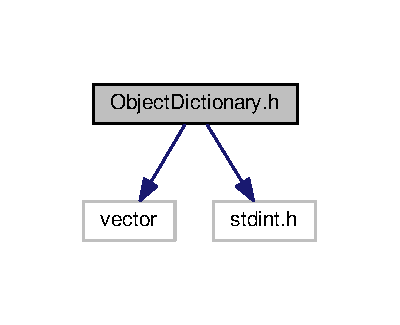
\includegraphics[width=192pt]{ObjectDictionary_8h__incl}
\end{center}
\end{figure}
This graph shows which files directly or indirectly include this file\+:
\nopagebreak
\begin{figure}[H]
\begin{center}
\leavevmode
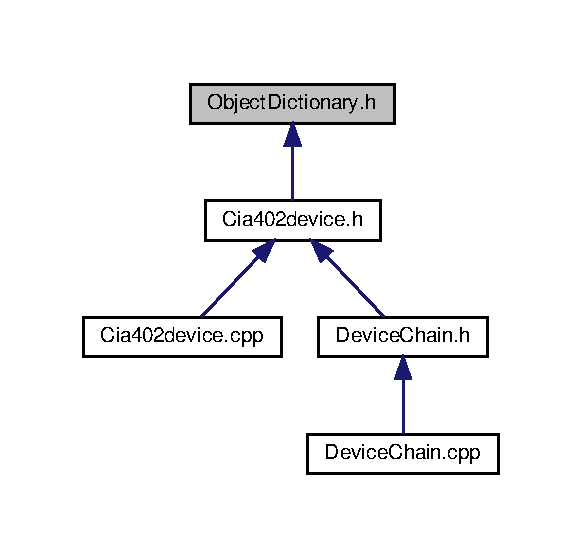
\includegraphics[width=280pt]{ObjectDictionary_8h__dep__incl}
\end{center}
\end{figure}
\subsection*{Namespaces}
\begin{DoxyCompactItemize}
\item 
 \hyperlink{namespaceod}{od}
\end{DoxyCompactItemize}
\subsection*{Variables}
\begin{DoxyCompactItemize}
\item 
const vector$<$ uint8\+\_\+t $>$ \hyperlink{namespaceod_acb23d3cf4cdb0ce0c85a884a5a97ac00}{od\+::controlword} =\{0x40,0x60\}
\item 
const vector$<$ uint8\+\_\+t $>$ \hyperlink{namespaceod_a7fe65fca00afb38d66fb49ec4fdc88c0}{od\+::statusword} =\{0x41,0x60\}
\item 
const vector$<$ uint8\+\_\+t $>$ \hyperlink{namespaceod_a75b2ed7fb6e21d4335334e1525fd223c}{od\+::commreset} =\{0x81\}
\item 
const vector$<$ uint8\+\_\+t $>$ \hyperlink{namespaceod_af9d6d0e820d6bc1ee375195e253f7b7b}{od\+::fullreset} =\{0x82\}
\item 
const vector$<$ uint8\+\_\+t $>$ \hyperlink{namespaceod_a5ca62a6451017dd2a0d53391d6fc5161}{od\+::start} =\{0x01\}
\item 
const vector$<$ uint8\+\_\+t $>$ \hyperlink{namespaceod_a360cf2eae7cc59f7bd224fcf5992c767}{od\+::goreadytoswitchon} =\{0x06,0x00\}
\item 
const vector$<$ uint8\+\_\+t $>$ \hyperlink{namespaceod_a933f995790a17f6cdd3b54df8f7483a6}{od\+::goswitchon} =\{0x07,0x00\}
\item 
const vector$<$ uint8\+\_\+t $>$ \hyperlink{namespaceod_a74448ee88df5960df4c32613e7cdcd53}{od\+::goenable} =\{0x0\+F,0x00\}
\item 
const vector$<$ uint8\+\_\+t $>$ \hyperlink{namespaceod_a12f3001ff096334fecb9c9749be4d1c2}{od\+::goswitchondisable} =\{0x00,0x00\}
\item 
const vector$<$ uint8\+\_\+t $>$ \hyperlink{namespaceod_af47128107b86d08e437f81d48d20b05a}{od\+::run} =\{0x1\+F,0x00\}
\item 
const vector$<$ uint8\+\_\+t $>$ \hyperlink{namespaceod_ae572be966c7d5de90544f2ac32dbbd38}{od\+::expedite} =\{0x3\+F,0x00\}
\item 
const vector$<$ uint8\+\_\+t $>$ \hyperlink{namespaceod_a9afdc654634df7cc336d824c594d484a}{od\+::quickstop} =\{0x02,0x00\}
\item 
const vector$<$ uint8\+\_\+t $>$ \hyperlink{namespaceod_a6f4fb30463057c20b9374a69826f6143}{od\+::\+Operation\+Mode} =\{0x60,0x60,0x00\}
\item 
const vector$<$ uint8\+\_\+t $>$ \hyperlink{namespaceod_a0469b45cd9158b638f0e0d6ed1102742}{od\+::\+Operation\+Mode\+Display} =\{0x61,0x60,0x00\}
\item 
const vector$<$ uint8\+\_\+t $>$ \hyperlink{namespaceod_a85efca0656a6714d7227858e112c4a73}{od\+::positionmode} =\{0x01\}
\item 
const vector$<$ uint8\+\_\+t $>$ \hyperlink{namespaceod_a2771fb30adf397c1cd2ddb092a414e82}{od\+::velocitymode} =\{0x03\}
\item 
const vector$<$ uint8\+\_\+t $>$ \hyperlink{namespaceod_ab5b4d34058d08a758277bf52cd31d8c9}{od\+::quick\+\_\+stop\+\_\+mode} =\{0x5\+A,0x60\}
\item 
const vector$<$ uint8\+\_\+t $>$ \hyperlink{namespaceod_af1bc07726906ffc6ea25ab9abb478143}{od\+::stop\+\_\+option\+\_\+code} =\{0x5\+D,0x60\}
\item 
const vector$<$ uint8\+\_\+t $>$ \hyperlink{namespaceod_ac4b980a10ae256ea019a767459b6ba9b}{od\+::checkerror} =\{0x02,0x10\}
\item 
const vector$<$ uint8\+\_\+t $>$ \hyperlink{namespaceod_a716df35f1a3cc3e1792c033be7fc0518}{od\+::positionaddress} =\{0x64,0x60,0x00\}
\item 
const vector$<$ uint8\+\_\+t $>$ \hyperlink{namespaceod_ad2c386d1f9bfc49b8a247f0b093f8963}{od\+::velocityactvalue} =\{0x69,0x60\}
\item 
const vector$<$ uint8\+\_\+t $>$ \hyperlink{namespaceod_adf45781fb80275c184d548ea793b376b}{od\+::velocityaddress} =\{0x69,0x60\}
\item 
const vector$<$ uint8\+\_\+t $>$ \hyperlink{namespaceod_a0bdcdb539c588cfae0d43cc0ba40ea05}{od\+::target\+\_\+position} =\{0x7\+A,0x60,0x00\}
\item 
const vector$<$ uint8\+\_\+t $>$ \hyperlink{namespaceod_a1d5963cb8a002987c96fae2e172790ee}{od\+::position\+\_\+demand} =\{0x62,0x60,0x00\}
\item 
const vector$<$ uint8\+\_\+t $>$ \hyperlink{namespaceod_a53c06ba9dc3fe72c8fd5fed43563a4a0}{od\+::torquemode} =\{0x\+F\+B\}
\item 
const vector$<$ uint8\+\_\+t $>$ \hyperlink{namespaceod_afc052d3983ca0866a0b8cd5d0fc5deaa}{od\+::torque\+\_\+type\+\_\+extern} =\{0x1\+D,0x20,0x00\}
\item 
const vector$<$ uint8\+\_\+t $>$ \hyperlink{namespaceod_ada58f32a60ef9137c7e9c4f4f54ace10}{od\+::torque\+\_\+online} =\{0x01,0x00\}
\item 
const vector$<$ uint8\+\_\+t $>$ \hyperlink{namespaceod_a3059829b7387e81bd7bad08c15364497}{od\+::torque\+\_\+target} =\{0x1\+C,0x20,0x00\}
\item 
const vector$<$ uint8\+\_\+t $>$ \hyperlink{namespaceod_afe81091f209f3c5eaf8f720e730900fa}{od\+::torque\+\_\+max} =\{0x72,0x60\}
\item 
const vector$<$ uint8\+\_\+t $>$ \hyperlink{namespaceod_aced8c17d62c0e774949057de0a99f402}{od\+::profile\+\_\+acceleration} =\{0x83,0x60,0x00\}
\item 
const vector$<$ uint8\+\_\+t $>$ \hyperlink{namespaceod_a57361a1a6b60fd8b93c2828fd7f5429f}{od\+::quick\+\_\+stop\+\_\+deceleration} =\{0x85,0x60,0x00\}
\item 
const vector$<$ uint8\+\_\+t $>$ \hyperlink{namespaceod_a5256e8439c66da9ab7ad06fa5f72ec1a}{od\+::motion\+\_\+profile\+\_\+type} =\{0x86,0x60\}
\item 
const vector$<$ uint8\+\_\+t $>$ \hyperlink{namespaceod_a47b7c8f6797cc134be5ee1d78d83ee50}{od\+::profile\+\_\+velocity} =\{0x81,0x60,0x00\}
\item 
const vector$<$ uint8\+\_\+t $>$ \hyperlink{namespaceod_a8d1e6a3e8180e5d64d68588ee182721c}{od\+::linear\+\_\+ramp\+\_\+trapezoidal} =\{0x00\}
\item 
const vector$<$ uint8\+\_\+t $>$ \hyperlink{namespaceod_a758ce0003cc482e5464959ed79c808e2}{od\+::target\+\_\+velocity} =\{0x\+F\+F,0x60,0x00\}
\item 
const vector$<$ uint8\+\_\+t $>$ \hyperlink{namespaceod_ace9cc22d0ccd7e2ac1b14fb14151ed73}{od\+::velocity\+\_\+encoder\+\_\+resolution\+\_\+num} =\{0x94,0x60,0x01\}
\item 
const vector$<$ uint8\+\_\+t $>$ \hyperlink{namespaceod_a2b157384b9a0fb00e80e99438f24f5de}{od\+::velocity\+\_\+encoder\+\_\+resolution\+\_\+den} =\{0x94,0x60,0x02\}
\item 
const vector$<$ uint8\+\_\+t $>$ \hyperlink{namespaceod_af615192e30bab04a02f1aa4c21a48642}{od\+::gear\+\_\+ratio} =\{0x91,0x60,0x00\}
\item 
const vector$<$ uint8\+\_\+t $>$ \hyperlink{namespaceod_a58009f80110aa4aff7a7ccd58037c27b}{od\+::aa} =\{0x71,0x60,0x00\}
\end{DoxyCompactItemize}

\hypertarget{PortBase_8cpp}{}\section{Port\+Base.\+cpp File Reference}
\label{PortBase_8cpp}\index{Port\+Base.\+cpp@{Port\+Base.\+cpp}}
{\ttfamily \#include \char`\"{}Port\+Base.\+h\char`\"{}}\\*
Include dependency graph for Port\+Base.\+cpp\+:
\nopagebreak
\begin{figure}[H]
\begin{center}
\leavevmode
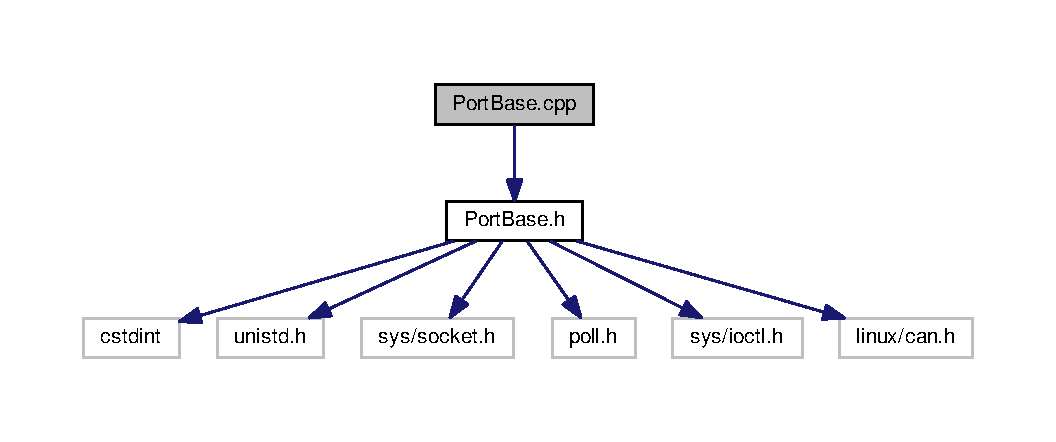
\includegraphics[width=350pt]{PortBase_8cpp__incl}
\end{center}
\end{figure}

\hypertarget{PortBase_8h}{}\section{Port\+Base.\+h File Reference}
\label{PortBase_8h}\index{Port\+Base.\+h@{Port\+Base.\+h}}
{\ttfamily \#include $<$cstdint$>$}\\*
{\ttfamily \#include $<$unistd.\+h$>$}\\*
{\ttfamily \#include $<$sys/socket.\+h$>$}\\*
{\ttfamily \#include $<$poll.\+h$>$}\\*
{\ttfamily \#include $<$sys/ioctl.\+h$>$}\\*
{\ttfamily \#include $<$linux/can.\+h$>$}\\*
Include dependency graph for Port\+Base.\+h\+:
\nopagebreak
\begin{figure}[H]
\begin{center}
\leavevmode
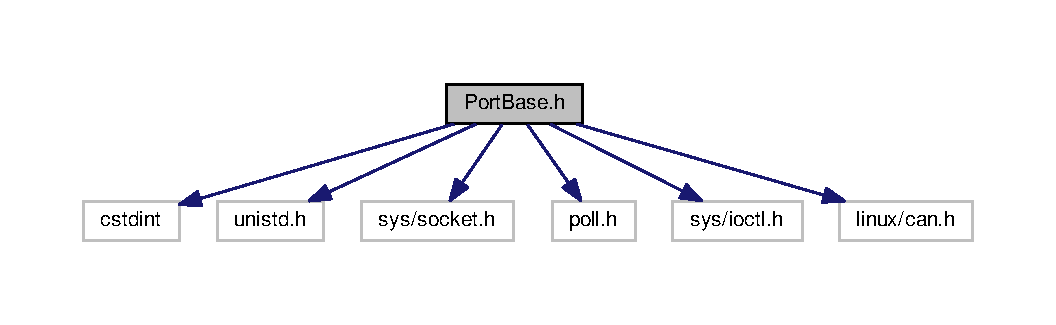
\includegraphics[width=350pt]{PortBase_8h__incl}
\end{center}
\end{figure}
This graph shows which files directly or indirectly include this file\+:
\nopagebreak
\begin{figure}[H]
\begin{center}
\leavevmode
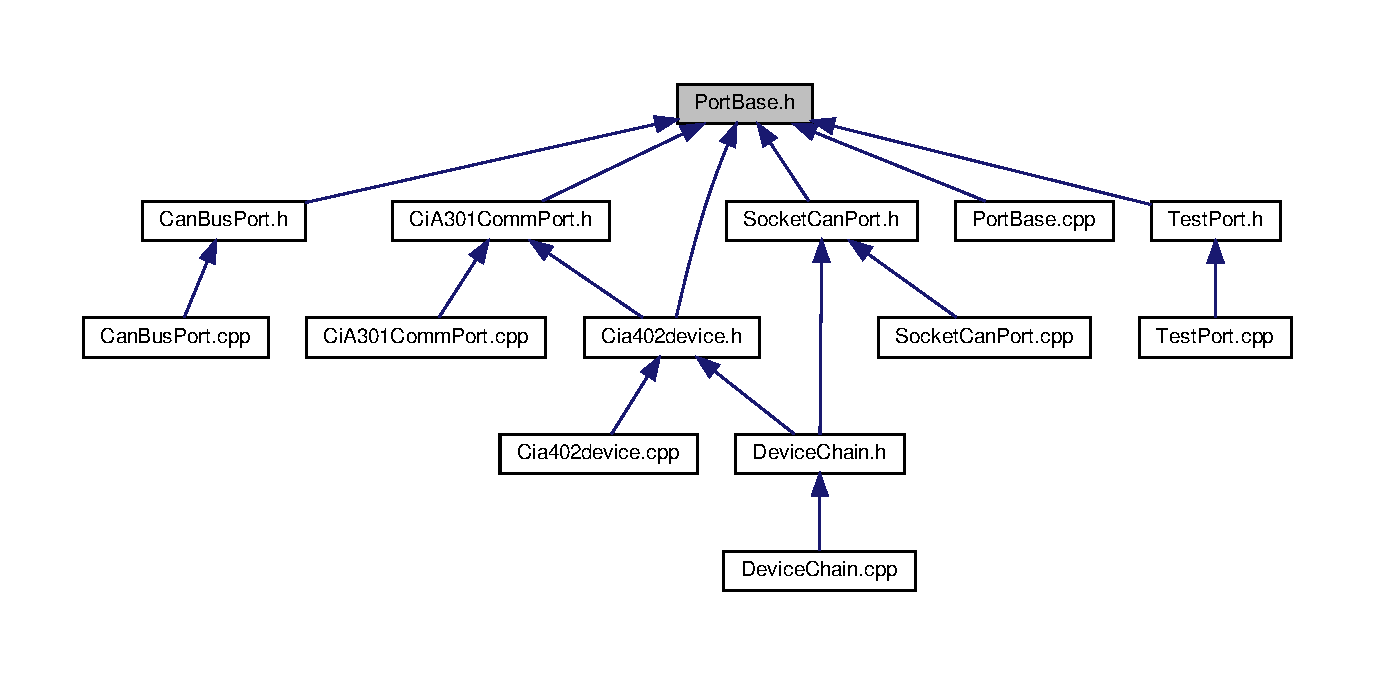
\includegraphics[width=350pt]{PortBase_8h__dep__incl}
\end{center}
\end{figure}
\subsection*{Classes}
\begin{DoxyCompactItemize}
\item 
class \hyperlink{classPortBase}{Port\+Base}
\end{DoxyCompactItemize}

\hypertarget{README_8md}{}\section{R\+E\+A\+D\+M\+E.\+md File Reference}
\label{README_8md}\index{R\+E\+A\+D\+M\+E.\+md@{R\+E\+A\+D\+M\+E.\+md}}

\hypertarget{SocketCanPort_8cpp}{}\section{Socket\+Can\+Port.\+cpp File Reference}
\label{SocketCanPort_8cpp}\index{Socket\+Can\+Port.\+cpp@{Socket\+Can\+Port.\+cpp}}
{\ttfamily \#include \char`\"{}Socket\+Can\+Port.\+h\char`\"{}}\\*
Include dependency graph for Socket\+Can\+Port.\+cpp\+:
\nopagebreak
\begin{figure}[H]
\begin{center}
\leavevmode
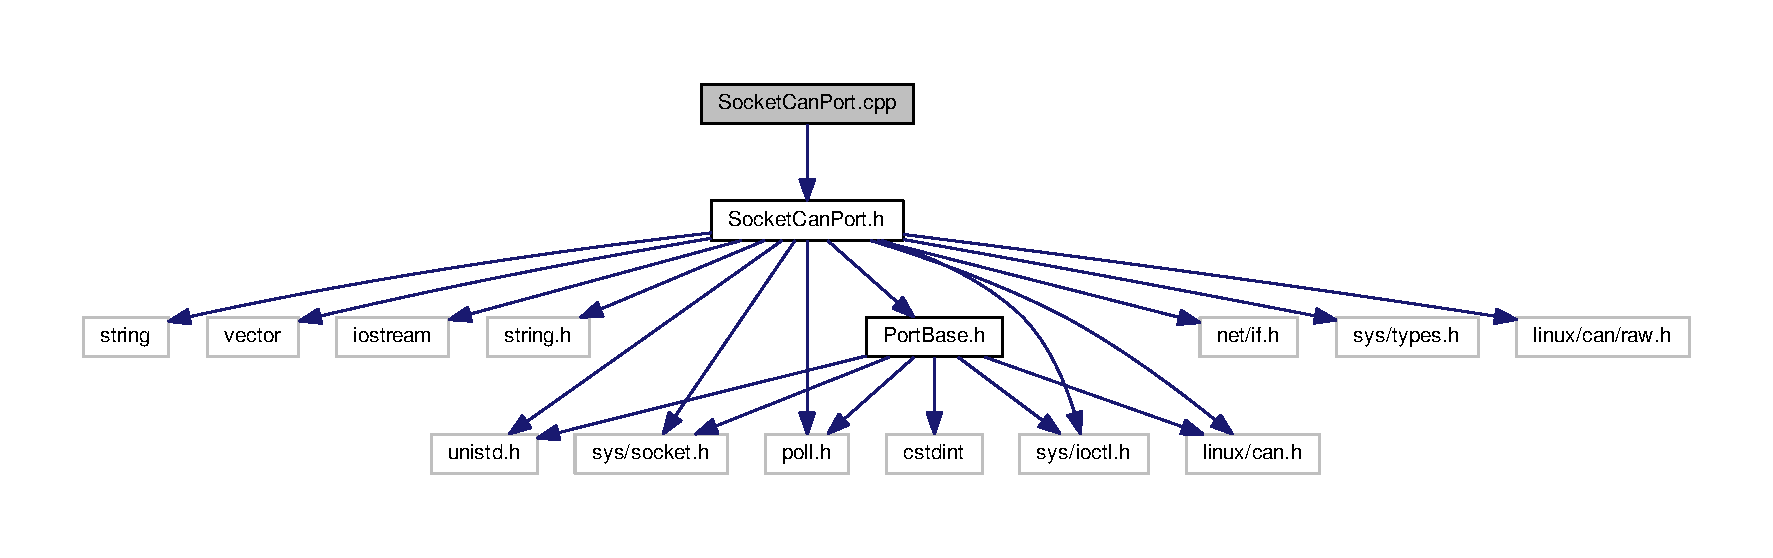
\includegraphics[width=350pt]{SocketCanPort_8cpp__incl}
\end{center}
\end{figure}

\hypertarget{SocketCanPort_8h}{}\section{Socket\+Can\+Port.\+h File Reference}
\label{SocketCanPort_8h}\index{Socket\+Can\+Port.\+h@{Socket\+Can\+Port.\+h}}
{\ttfamily \#include $<$string$>$}\\*
{\ttfamily \#include $<$vector$>$}\\*
{\ttfamily \#include $<$iostream$>$}\\*
{\ttfamily \#include $<$string.\+h$>$}\\*
{\ttfamily \#include $<$unistd.\+h$>$}\\*
{\ttfamily \#include $<$net/if.\+h$>$}\\*
{\ttfamily \#include $<$sys/types.\+h$>$}\\*
{\ttfamily \#include $<$sys/socket.\+h$>$}\\*
{\ttfamily \#include $<$poll.\+h$>$}\\*
{\ttfamily \#include $<$sys/ioctl.\+h$>$}\\*
{\ttfamily \#include $<$linux/can.\+h$>$}\\*
{\ttfamily \#include $<$linux/can/raw.\+h$>$}\\*
{\ttfamily \#include \char`\"{}Port\+Base.\+h\char`\"{}}\\*
Include dependency graph for Socket\+Can\+Port.\+h\+:
\nopagebreak
\begin{figure}[H]
\begin{center}
\leavevmode
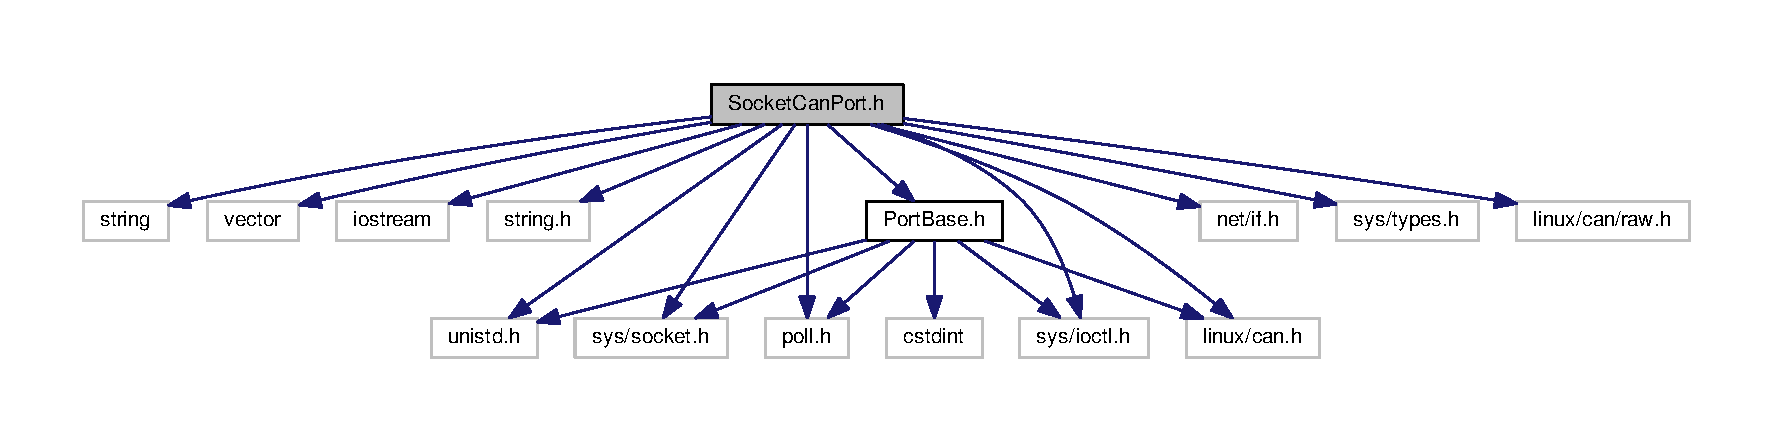
\includegraphics[width=350pt]{SocketCanPort_8h__incl}
\end{center}
\end{figure}
This graph shows which files directly or indirectly include this file\+:
\nopagebreak
\begin{figure}[H]
\begin{center}
\leavevmode
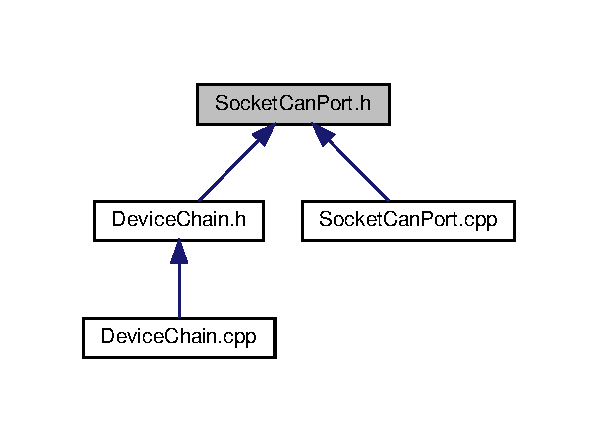
\includegraphics[width=287pt]{SocketCanPort_8h__dep__incl}
\end{center}
\end{figure}
\subsection*{Classes}
\begin{DoxyCompactItemize}
\item 
class \hyperlink{classSocketCanPort}{Socket\+Can\+Port}
\end{DoxyCompactItemize}

\hypertarget{TestPort_8cpp}{}\section{Test\+Port.\+cpp File Reference}
\label{TestPort_8cpp}\index{Test\+Port.\+cpp@{Test\+Port.\+cpp}}
{\ttfamily \#include \char`\"{}Test\+Port.\+h\char`\"{}}\\*
Include dependency graph for Test\+Port.\+cpp\+:
\nopagebreak
\begin{figure}[H]
\begin{center}
\leavevmode
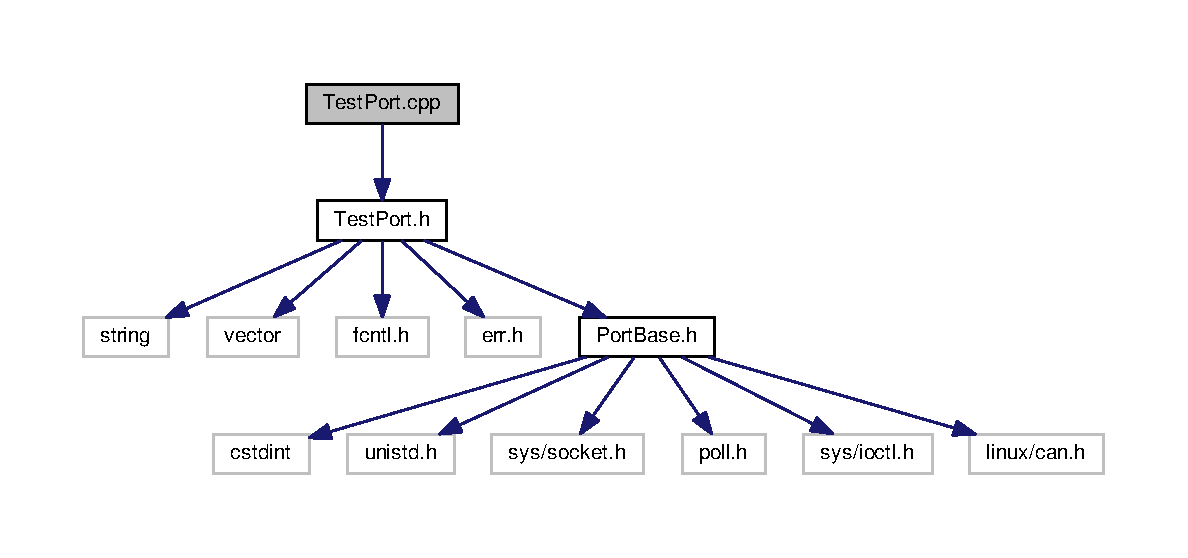
\includegraphics[width=350pt]{TestPort_8cpp__incl}
\end{center}
\end{figure}

\hypertarget{TestPort_8h}{}\section{Test\+Port.\+h File Reference}
\label{TestPort_8h}\index{Test\+Port.\+h@{Test\+Port.\+h}}
{\ttfamily \#include $<$string$>$}\\*
{\ttfamily \#include $<$vector$>$}\\*
{\ttfamily \#include $<$fcntl.\+h$>$}\\*
{\ttfamily \#include $<$err.\+h$>$}\\*
{\ttfamily \#include \char`\"{}Port\+Base.\+h\char`\"{}}\\*
Include dependency graph for Test\+Port.\+h\+:
\nopagebreak
\begin{figure}[H]
\begin{center}
\leavevmode
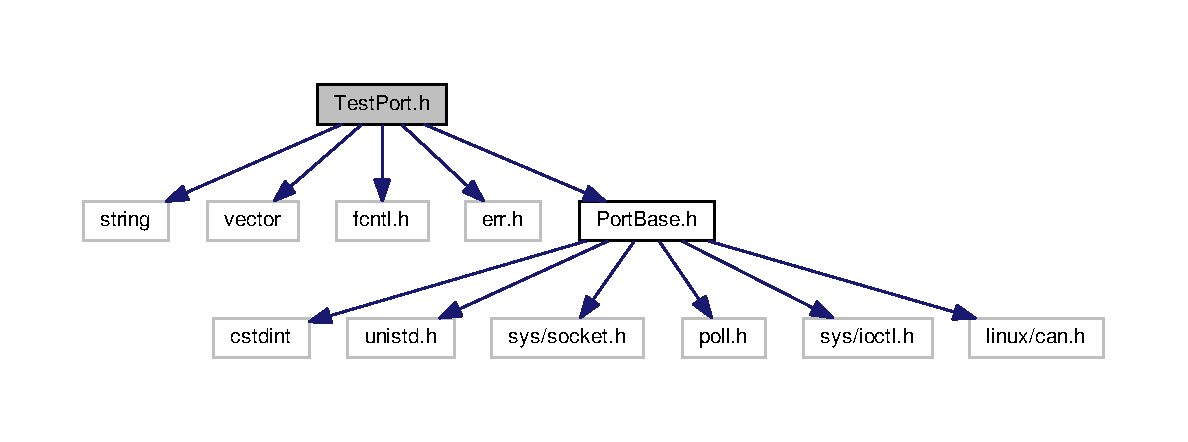
\includegraphics[width=350pt]{TestPort_8h__incl}
\end{center}
\end{figure}
This graph shows which files directly or indirectly include this file\+:
\nopagebreak
\begin{figure}[H]
\begin{center}
\leavevmode
\includegraphics[width=153pt]{TestPort_8h__dep__incl}
\end{center}
\end{figure}
\subsection*{Classes}
\begin{DoxyCompactItemize}
\item 
class \hyperlink{classTestPort}{Test\+Port}
\end{DoxyCompactItemize}

%--- End generated contents ---

% Index
\backmatter
\newpage
\phantomsection
\clearemptydoublepage
\addcontentsline{toc}{chapter}{Index}
\printindex

\end{document}
